%======================================================================
%   Zak Webb
%   Ph. D. Thesis
%   Department of Physics and Astronomy
%   University of Waterloo
% 
%   Ground energy of multi-particle quantum walk
%======================================================================


\documentclass[../thesis-main/thesis-main]{subfiles}
\begin{document}

\chapter{Ground energy of multi-particle quantum walk}
\label{chap:MP_ground}


%\section{Introduction}
%%%%%%%%%%%%%%%%%%%%%%%%%%%%%%%%%%%%%%%%%%%%%%%%%%%%%%%%%%%%%%%%%%

With our proof that the ground energy problem for a single-particle quantum walk is \QMA-complete, we will now investigate the related problem for MPQW.  The similarities between the two systems, as well as the well-known difficulty in analyzing many-body systems, gives good intuition that this problem is hard, but the actual proof requires a lot of detail.

In particular, the \QMA-hardness proof for quantum walk was relatively straightforward, as the requisite circuit-to-Hamiltonian mapping is a simple extension to well-known techniques.  Further, we understand the dynamics of the Hamiltonians derived from a given circuit, leading to exact solutions for the energies.  With the MPQW, a full analysis of the dynamics is currently beyond our knowledge, and our universality construction from \chap{MP_universality} relied on a reduction to the cases with at most two interacting particles.  In order to show that finding the ground energy of a MPQW is \QMA-hard, our techniques will again heavily rely on the cases with a small number of particles.

Our proof of \QMA-hardness will actually show that the the MPQW ground energy problem is \QMA-hard when restricted to instances where the ground state nearly minimizes both the interaction and movement terms of the Hamiltonian.  By restricting ourselves to these frustration-free states, we will show that ground state is nearly contained within the span of single-particle states that don't overlap.  With this restriction, we will still have correlations between many particles, but we will be able to perform an analysis using only a bounded number of particles.  

In particular, we will construct a basic graph $g_0$ that only supports single-particle states in our frustration-free subspace.  We then connect these graphs to build more complicated entanglement structure between particles, until we construct graphs for which the n-particle frustration-free ground space contains an encoded subspace of history states, plus some unwanted states.  We then show how to transform a given graph to remove these unwanted states from the ground space, without changing the energy gap greatly.

Our proof strategy, using repeated applications of the Nullspace Projection Lemma (\lem{npl}), is analogous to that of reference \cite{KKR04}, where the so-called Projection Lemma was used similarly. Our technique has the advantage of not requiring the terms we add to our Hamiltonian to have ``unphysical'' problem-size dependent coefficients (it also has this advantage over the method of perturbative gadgets \cite{KKR04}). This allows us to prove results about the ``physically realistic'' Bose-Hubbard Hamiltonian. A similar technique based on Kitaev's Geometric Lemma was used recently in reference \cite{GN13} (however, that method is slightly more computation intensive, requiring a lower bound on $\gamma(H_{B})$ as well as bounds on $\gamma(H_{A})$ and $\gamma(H_{B}|_{S})$).

Additionally, note that this chapter is essentially a combination of Childs, Gosset, and Webb's \cite{BHQMA} and \cite{XYQMA}.  In particular, the proof structure is identical to that of \cite{BHQMA}, with some modifications to the proof that arose in \cite{XYQMA}.  However, the previous results only applied to onsite-interactions corresponding to the Bose-Hubbard model with positive interactions.  The proof in this chapter is a generalization to arbitrary positive-semidefinite constant-range interactions.

%%%%%%%%%%%%%%%%%%%%%%%%%%%%%%%%%%%%%%%%%%%%%%%%%%%%%%%%%%%%%%%%%%
\section{MPQW Hamiltonian ground-energy problem}

Before we begin constructing various graphs, and determining the eigenvalues of the MPQW on these graphs, it will be useful to define the problem statement that we want to prove hard.  Along these lines, we will also need to determine the interactions for which our proof will hold.

Our proof strategy heavily relies on combining positive-semidefinite matrices, and analyzing the resulting ground space and eigenvalue gaps.  Additionally, we will often want to guarantee that adding a particle to a given graph can only increase its energy.  These are all the requirements we discussed in \sec{MPQW_pos} in \chap{MPQW}.

Along these lines, let $\mathcal{U}$ be an interaction with maximum range $\dmax$, satisfying the conditions that for all $0\leq d\leq \dmax$ and all $x,y\in \NN^+$,
\begin{align}
  0 \leq \mathcal{U}_d(x,y) \leq \mathcal{U}_d(x+1,y).
\end{align}
We also want to guarantee that there exists two constants $\gamma$ and $\nu$ such that $\Vert H_{\mathcal{U},G}^N \Vert \leq \gamma N^\nu$, so that the energy can only grow polynomially.  With these interactions, we can now construct the problem of interest. 

\begin{problem}[$\mathcal{U}$-interaction MPQW Hamiltonian]
  Given as input a $K$-vertex graph $G$, a number of particles $N$, a real number $c$, and a precision parameter $\epsilon = 1/T$, where the positive integers $N$ and $T$ are given in unary, and the graph $G$ is given as its adjacency matrix (a $K\times K$ symmetric $0$-$1$ matrix), the $\mathcal{U}$-interaction MPQW Hamiltonian problem is to determine whether the smallest eigenvalue of $H_{\mathcal{U},G}^N$ is at most $c$ or is at least $c+\epsilon$, with a promise that one of these two cases hold.
\end{problem}

Note that we can modify this problem statement to only include symmetric (or anti-symmetric) states, and it will be called the $\mathcal{U}$-interaction (anti-)symmetric MPQW Hamiltonian problem.


%%%%%%%%%%%%%%%%%%%%%%%%
\subsection{MPQW Hamiltonian is contained in \QMA}
\label{sec:containment_in_QMA}

The proof that the $\mathcal{U}$-interaction MPQW Hamiltonian problem is contained in \QMA is rather straightforward, since we can simulate evolution by the Hamiltonian $H_{\mathcal{U},G}^N$, as was shown in \chap{MPQW}.  In particular, we can use phase estimation in order to approximate the energy with high probability.

More concretely, we are given an instance specified by $G$, $N$, $c$, and $\epsilon$. We are also given an input state $|\phi\rangle$ of $n_{\text{input}}$ qubits, where $n_{\text{input}}=\lceil \log_{2}|V(G)|^N\rceil $.  Note that $n_{\text{input}}=\mathcal{O}(N\log\left(K\right))$, where $K=|V|$ is the number of vertices in the graph $G$. We embed $\CC^{|V(G)|^N}$ into the space of $n_{\text{input}}$ qubits straightforwardly as the subspace spanned by the first $|V(G)|^N$ standard basis vectors (with lexicographic ordering, say). 

The first step of the verification procedure is to measure $H_{\mathcal{U},G}^{N}$ in the state $|\phi^{\prime}\rangle$. The Hamiltonian $H_{\mathcal{U},G}^{N}$ is sparse and efficiently row-computable, with norm
\begin{equation}
  \left\Vert H_{G}^{N}\right\Vert \leq \gamma N^\nu.
\end{equation}
We use phase estimation (see for example \cite{CEMM98}) to estimate the energy of $|\phi\rangle$, using sparse Hamiltonian simulation \cite{AT03} to approximate evolution according to $H_{\mathcal{U},G}^{N}$. We choose the parameters of the phase estimation so that, with probability at least $\frac{2}{3}$, it produces an approximation $E$ of the energy with error at most $\frac{\epsilon}{4}$. This can be done in time $\poly(N,K,\frac{1}{\epsilon})$. If $E\leq c+\frac{\epsilon}{2}$ then we accept; otherwise we reject.

We now show that this verification procedure satisfies the completeness and soundness requirements of \defn{QMA}. For a yes instance, an eigenvector of $H_{\mathcal{U},G}^{N}$ with eigenvalue $e\leq c$ is accepted by this procedure as long as the energy $E$ computed in the phase estimation step has the desired precision. To see this, note that we measure $\left|E-e\right|\leq\frac{\epsilon}{4}$, and hence $E\leq c+\frac{\epsilon}{4}$, with probability at least $\frac{2}{3}$.  For a no instance, the value $E$ computed by the phase estimation step satisfies $E\geq c+\frac{3\epsilon}{4}$ with probability at least $\frac{2}{3}$, in which case the state is rejected. From this we see that the probability of accepting a no instance is at most $\frac{1}{3}$.

Note that the problem remains in \QMA when we restrict ourselves to the (anti-)symmetric subspace.  The verification procedure remains nearly the same, except that we measure a projector onto the (anti-)symmetric subspace on $\ket{\phi}$ before we perform phase estimation.  In a yes case, Merlin provides an (anti-)symmetric state, and this test always passes.  In a no case, if this test passes, we are then checking the energy of an (anti-)symmetric state, which fails the energy test with high probability.

With all of this, we then have that the $\mathcal{U}$-interaction MPQW Hamiltonian problem is contained within \QMA.


%%%%%%%%%%%%
\subsection{\QMA-hard problem}

While the $\mathcal{U}$-interaction MPQW Hamiltonian problem is the natural problem relating to the ground energy of a MPQW, we will prove that a restricted version of this problem is \QMA hard.  Namely, if we restrict ourselves to those Hamiltonians that minimize both the interaction and movement terms, we can more easily analyze the $N$-particle ground space.

As such, remember from \chap{MPQW} that for a given graph $G$, we define the positive-semidefinite matrix $H_{\mathcal{U}}(G,N)$ by
\begin{align}
  H_{\mathcal{U}}(G,N) &= \sum_{w=1}^{N} \big( A(G) - \mu(G)\big)^{(w)} + \sum_{d=0}^{\dmax} \sum_{\substack{u,v\in V(G)\\d(u,v) = d}} \mathcal{U}_d(\hat{n}_u,\hat{n}_v),
\end{align}
and that $\lambda_N^i(G)$ is the $i$-th smallest eigenvalue of $H_{\mathcal{U}}(G,N)$.

\begin{problem}[Frustration-free $\mathcal{U}$-interaction MPQW Hamiltonian]
  We are given as input a $K$-vertex simple graph $G$, a number of particles $N\leq K$, and a precision parameter $\epsilon = 1/T$, where the positive integers $N$ and $T \geq 4K$ are given in unary, and the graph $G$ is given as its adjacency matrix (a $K\times K$ symmetric $0$-$1$ matrix). We are promised that either $\lambda_N^1(G) \leq \epsilon$ (a yes instance), or else that $\lambda_N^1(G) \geq 2\epsilon $ (a no instance) and we are asked to decide which is the case.
\end{problem}

Note that this is a special case of the $\mathcal{U}$-interaction MPQW Hamiltonian, with $c = N\mu(G) + \epsilon$.  As such, if we show that the Frustration-free $\mathcal{U}$-interaction MPQW Hamiltonian problem is \QMA-hard, we will also show that the non-frustration-free problem is \QMA-complete.

%%%%%%%%%%%%%%%%%%%%%%%%%%%%%%%%%%%%%%%%%%%%%%%%%%%%%%%%%%%%%%%%%%
\section{Useful graph primitives}\label{sec:graph_primitives}

At this point, we will want to construct the graph for which our \QMA-hardness result will hold.  As such, we will at this point restrict our attention to a particular interaction, $\mathcal{U}$ and omit the corresponding subscripts.  While the idea behind the construction of these graphs will not change depending on the interaction, the exact graph we construct will depend on the largest distance for which there is a non-zero interaction.  We will want to construct a foundational graph that does not have a two-particle ground state, and also we will want to ensure that any connections between these building blocks in the larger graphs will only allow for particular interactions.

Let us then assume that the minimum distance that the interaction $\mathcal{U}$ has non-zero interactions is $\dmin$, while the maximum distance is $\dmax$.  Our graph will only depend on $\dmax$, but it will be useful to also know $\dmin$.  We will also assume that $\mathcal{U}_{\dmin}^{(1,1)} > 0$, so that there is some energy penalty if two particles are at a distance $\dmin$ (assuming that $\dmin > 0$ --- otherwise we will assume that $\mathcal{U}_0^{2} > 0$).

Additionally, we will want the eventual graph to be a simple graph, so that there is always at most a single edge between two vertices and no self-loops.  Unfortunately, our proof strategy will involve adding many positive semi-definite terms to the adjacency matrix, which correspond to adding in edges and self-loops.  As such, we will instead force every vertex in the graph to contain a self-loop, so that by removing all of the self loops we only shift the energy levels by a constant amount.  Keep this in mind, as the eventual graph is defined.

With all of this said, however, this section only define some useful building blocks that will be used in the final construction of the graph for a given circuit.  All of these graphs will be constant sized, and we will show a spanning set for their single-particle and two-particle ground states.  By construction, they will not have any three-particle frustration-free states.

%%%%%%%%%%%%%%%
\subsection{Gate graphs}\label{sec:gate_graphs}


\todo{rewrite this introduction}
In this section we define a class of graphs (\emph{gate graphs}) and a diagrammatic notation for them (\emph{gate diagrams}) that will allow us to more easily construct the graphs that will be used in our proofs.  Additionally, we will also discuss the MPQW Hamiltonian acting on these graphs, with a particular emphasis on the low-energy states.  We will eventually use this characterization of the low energy states on these small graphs to analyze and give bounds on the low energy states of the more complicated graphs corresponding to particular gate diagrams.

Every gate graph is constructed using a specific, finite-sized graph $g_{0}$ as a building block that only depends on the interaction range of the interaction Hamiltonian for the MPQW.  This building block is shown in \fig{g_0} (in the specific instance of for graphs with $\dmin <= 1$ and discussed in \sec{g_0_graph}).  These graphs are designed so that in the low energy sector, each copy of $g_0$ can only contain a single particle at a time, so that we can force particles to occupy certain states.  Additionally, the low energy states correspond to the history states of a simple single-qubit circuits, as described in \chap{SP_universality}.

\todo{fix this part}
In \sec{FF_State} we discuss the ground states of the Bose-Hubbard model on gate graphs. For any gate graph $G$, the smallest eigenvalue $\mu(G)$ of the adjacency matrix $A(G)$ satisfies $\mu(G)\geq-1-3\sqrt{2}$. It is convenient to define the constant
\begin{equation}
e_{1}=-1-3\sqrt{2}.\label{eq:e1_defn}
\end{equation}
When $\mu(G)=e_{1}$ we say $G$ is an $e_{1}$-gate graph. We focus on the frustration-free states of $e_1$-gate graphs (recall from \defn{FF_states} that $|\phi\rangle\in \mathcal{Z}_N(G)$ is frustration free iff $H(G,N)|\phi\rangle=0$). We show that all such states live in a convenient subspace (called $\mathcal{I}(G,N)$) of the $N$-particle Hilbert space. This subspace has the property that no two (or more) particles ever occupy vertices of the same copy of $g_{0}$. The restriction to this subspace makes it easier to analyze the ground space.

In \sec{Occupancy-constraints} we consider a class of subspaces that, like $\mathcal{I}(G,N)$, are defined by a set of constraints on the locations of $N$ particles in an $e_{1}$-gate graph $G$. We state an ``Occupancy Constraints Lemma'' (proven in \app{Occupancy-Constraints-Lemma}) that relates a subspace of this form to the ground space of the Bose-Hubbard model on a graph derived from $G$.


\subsubsection{The graph $g_0$}\label{sec:g_0_graph}

The graph $g_{0}$ shown in \fig{g_0} is constructed using the method of \chap{SP_ground}, with the single qubit circuit corresponding to a sequence of $H$ and $HT$ gates.  The intuition behind this graph is to force the ground state to correspond to the history state of these simple computations, thus allowing us to reference the computational value of the corresponding qubit in several disparate locations.  We will eventually combine several of these $g_0$ graphs using projectors, which will remove certain states from the ground space depending on the value of the corresponding qubits.

As such, let $k = 4 + 2 \lfloor \frac{\dmax}{2}\rfloor$, and then let us look at the single-qubit circuit $\mathcal{C}_0$ with $k$ gates $U_j$, for $j\in[k]$, where 
\begin{align}
U_{1}=HT\qquad U_{2}=\left(HT\right)^{\dagger}
\end{align}
and the rest of the $U_j=H$.  We will use the second, third, and fourth of these time steps as computations in the eventual gadgets, while the remaining time steps act as padding to ensure that the computational time steps used in the eventual graph occur at a distance at least $\dmax$ from each other.  As the circuit $\mathcal{C}_0$ implements an identity operation, we can easily concatenate several of these circuits and examine the graph corresponding to the circuit using circular time, as in the construction used in \chap{SP_ground}.  For our purposes, we will want to use 8 copies of $\mathcal{C}_0$ in series, as the eventual gadgets used in our proof have 8 possible locations for interactions with other copies of $g_0$.

In particular, we will have that the $0$-$1$ Hamiltonian corresponding to the eventual adjacency matrix of $g_0$ acts on the Hilbert space $\mathcal{H}(g_0) = \CC^{2}\otimes \CC^{8k} \otimes \CC^8$.  If we then remember that $B(U)$ is the operator that takes $\omega \mapsto S$, where $\omega = e^{i \pi/4}$ and  $S$ is the shift operator acting on $\CC^{8}$, we have that the component of the Hamiltonian corresponding to the circuit is
\begin{equation}
  H_{\text{prop}} = -\sqrt{2} \sum_{t=0}^{8k-1} B(V_{t})_{13} \otimes \ketbra{t+1}{t} + B(V_{t}^\dag)_{13} \otimes \ketbra{t}{t+1},
\end{equation}
where the $B(U)_{13}$ act on the Hilbert spaces $\CC^{2}\otimes \CC^{8}$ while the clock acts on the $\CC^{8k}$ Hilbert space, and where
\begin{equation}
  V_t = \begin{cases}
    HT & t = 0 \mod 8\\
    (HT)^{\dag} & t = 1 \mod 8\\
    H & \text{otherwise}.
  \end{cases}
\end{equation}
This term, along a penalty to the $\CC^8$ Hilbert space given by
\begin{equation}
  H_{\text{pen}} = \II_{\CC^2} \otimes \II_{\CC^{8k}} \otimes \big( S^3 + S^4 + S^3\big),
\end{equation}
which forces the third register into a particularly useful state, allows us to guarantee that the ground state is a history state.  Altogether, we then have that the adjacency matrix of $g(0)$ is given by
\begin{equation}
  A(g_0) = H_{\text{prop}} + H_{\text{pen}},
\end{equation}
where each vertex is labeled by a computational basis state in the Hilbert space, namely $(z,t,j)$ with $z\in \FF_2$, $t\in [8k]$, and $j\in[8]$.  The graph $g_0$ in the special case that $\dmax = 0$ is shown in \fig{g_0}.

%%%%%%%
\begin{figure}
  \centering
  \tikzsetnextfilename{MP_g_0}
  \input{../tikz/MP_G_0.tex}
  \caption[The graph $g_0$]{The graph $g_{0}$ for the case $\dmax \leq 1$.  Vertices are arranged with each ray corresponding to a specific time $t$ proceeding clockwise, with the outer 8 vertices corresponding to logical $0$ and the inner 8 corresponding to logical $1$, with the further breakdown into 8 vertices corresponding to the ancillary register.  The difference in color for some edges is an attempt to highlight those edges corresponding to the penalty term (bottom of the figure) and the circuit (top left of the figure).  \label{fig:g_0}}
\end{figure}

We can then use the results of \chap{SP_ground} to calculate the smallest eigenvalue of $A(g_0)$, the corresponding eigenvectors, and the eigenvalue gap.  In particular, we have that the smallest eigenvalue is 
\begin{equation}
  e_1 = -1 - 3 \sqrt{2} = -5.24\ldots, \label{eq:e_1},
\end{equation}
corresponding to a four dimensional ground space spanned by the states
\begin{align}
  \ket{\psi_{z,0}} &= \frac{1}{\sqrt{8k}}\sum_{t=0}^{8k-1} \big(V_t V_{t-1} \cdots V_1\big) \ket{z} \ket{t} \ket{\omega}= \frac{1}{\sqrt{8k}}\sum_{t'=0}^{4k-1} \ket{z} \ket{2t'}\ket{\omega} + V_{2t' + 1} \ket{z} \ket{2t'+1}\ket{\omega}\label{eq:psi0m}\\
  \ket{\psi_{z,1}} &= \frac{1}{\sqrt{8k}} \sum_{t'=0}^{4k-1} \ket{z}\ket{2t'} \ket{\overline{\omega}} + V_{2t'+1}* \ket{z} \ket{2t'+1} \ket{\overline{\omega}}\label{eq:psi1m},
\end{align}
where
\begin{align}
  \ket{\omega} &= \frac{1}{\sqrt{8}} \sum_{j=0}^{7} e^{i \pi j/4} \ket{j} &\text{ and } &&
  \ket{\overline{\omega}} &= \frac{1}{\sqrt{8}} \sum_{j=0}^7 e^{-i \pi j/4} \ket{j}.
\end{align}
Additionally, we have that the energy gap is at least 
\begin{equation}
  \lambda_1^2(g_0) \geq \sqrt{2} \cos\Big(\frac{\pi}{4k}\Big) \geq \frac{\pi\sqrt{2}}{16 k^2} = c_k,
\end{equation}
which is constant for all interactions with a given $\dmax$.



Note that the amplitudes of $|\psi_{z,0}\rangle$ in the above basis contain the result of computing either the identity, Hadamard, or $HT$ gate acting on the ``input'' state $|z\rangle$, while the amplitudes $\ket{\psi_{z,1}}$ corresponds to the result of the identity, Hadamard or $\overline{HT}$ gate acting on the ``input'' state.  Additionally, this information is repeated at least $8$ times, once for each copy of $\mathcal{C}_0$.


With these bounds on the single particle eigenvalues and their corresponding eigenstates, we can now show that the graph $g_{0}$ has no two-particle frustration-free states. By \lem{increase_part_number}, it follows that $g_0$ has no $N$-particle frustration-free states for $N\geq 2$.  While we would like this to be true for all interactions, in the case of only onsite interactions ($\dmax =0$) no anti-symmetric state is penalized and thus there is a $4$-particle frustration-free state.  However, we show that this is the only case for which this is true, and further that if we restrict ourselves to the symmetric subspace, we again have that there are no frustration-free two-particle states.

\begin{lemma}
\label{lem:2particle}If $\dmax > 0$, then $\lambda_{2}^{1}(g_{0})>0$ for all states.  If $\dmax = 0$, then when restricted to symmetric states, $\lambda_2^{1}(g_0) >0$.
\end{lemma}

\begin{proof}
Suppose (for a contradiction) that $|Q\rangle\in \HHH(g_0)^{\otimes 2}$ is a nonzero vector in the nullspace of $H(g_{0},2)$, so 
\begin{equation}
  H_{g_{0}}^{2}|Q\rangle
    =\bigg(A(g_{0})\otimes\II+\II\otimes A(g_{0})+\sum_{i,j \in g_{0}}\mathcal{U}_{d(i,j)}(\hat{n}_i,\hat{n}_j)\bigg)|Q\rangle=2e_{1}|Q\rangle.
\end{equation}
This implies 
\begin{equation}
  A(g_{0})\otimes\II|Q\rangle=\II\otimes A(g_{0})|Q\rangle=e_{1}|Q\rangle
\end{equation}
since $A(g_0)$ has smallest eigenvalue $e_1$ and the interaction term is positive semidefinite. We can therefore write 
\begin{equation}
  |Q\rangle=\sum_{z,a,x,y\in \FF_2}Q_{za,xy}|\psi_{z,a}\rangle|\psi_{x,y}\rangle
\end{equation}
and 
\begin{equation}
  \mathcal{U}_{d(u,v)}(\hat{n}_u,\hat{n}_v)|Q\rangle=0
\end{equation}
for all vertices $u,v\in g_{0}.$ 


We then have by assumption that  $\mathcal{U}^{(1,1)}_{\dmax} >  0$ if $\dmax > 0$ or $\mathcal{U}^{2}_{0} > 0$ if $\dmax = 0$,  and thus for all vertices $u,v$ of distance $\dmax$, 
\begin{equation}
  \braket{u,v}{Q} = 0\label{eq:dmin_annihilate}.
\end{equation}
We will use this equation to show a contradiction, so that $\ket{Q}$ cannot exist.

Note that vertices of the form $(x,T,j)$ and $(z,T+t,k)$ are at least a distance $t$ apart for all times $t < 4 k$, since edges only connect vertices with corresponding times that differ by at most 1.  Further, note that the portion of the Hamiltonian that connect adjacent times only arise from the terms corresponding to the circuit.  Since each unitary for $k > t\geq 2$ corresponds to a Hadamard, and the corresponding term in the Hamiltonian only connects vertices with the same $j$ or $j$'s that differ by 4, we have that only vertices of the form $(x,2,j)$ and $(z,2+t,j)$ or $(x,2,j)$ and $(z,2+t,j+4)$ can be a distance $t$ apart; all other pairs of vertices with these two times must be at a distance of at least $t+1$.

With all of this in mind, let us assume that $\dmax$ is an even integer greater than zero.  We then have that the vertices $(0,2,j)$ and $(0,1+\dmax,j+4)$ are a distance $\dmax-1$ apart.  Further, we have that $(0,1+\dmax,j+4)$ is also connected to the vertices $(0,1+\dmax,j+1)$ and $(0,1+\dmax,j-1)$ (from the penalty term of the Hamiltonian), and thus we have that the vertices $u = (0,2,j)$ and $v = (0,1+\dmax, j + \ell)$ are a distance $\dmax$ apart for all $j\in [8]$ and for $\ell = \pm 1$.  Using \eq{dmin_annihilate} with these pairs of vertices we then have that 
\begin{align}
  \braket{u,v}{Q} &= \sum_{x,a,z,b\in \FF_2} Q_{xa,zb} \braket{0,2,j}{\psi_{x,a}}\braket{0,1+\dmax,j+\ell}{\psi_{zb}}\\
  &=\frac{1}{64 k} \sum_{x,a,z,b\in \FF_2} Q_{xa,zb} \braket{0}{x} \bra{0} H \ket{z} \omega^{(-1)^a j+ (-1)^b (j+\ell)}\\
  &= \frac{1}{64\sqrt{2}k} \big( (Q_{00,00} + Q_{00,10}) \omega^{2j + \ell} + (Q_{00,01} + Q_{00,11})\omega^{-\ell} \nonumber\\
  &\qquad \qquad + (Q_{01,00} + Q_{01,10})\omega^{\ell} + (Q_{01,01} + Q_{01,11})\omega^{-2j - \ell}\big),
\end{align}
and thus we have that $Q_{0a,0b} = - Q_{0a,1b}$ for all $a,b\in \FF_2$.  Using the same reasoning with vertices $u =(0,2,j)$ and $v =(1,1+\dmax, j+\ell)$ with $\ell =\pm 1$ then gives us 
\begin{align}
  \braket{u,v}{Q} &= \sum_{x,a,z,b\in \FF_2} Q_{xa,zb} \braket{0,2,j}{\psi_{x,a}}\braket{1,\dmax,j+\ell}{\psi_{zb}}\\
  &=\frac{1}{64 k} \sum_{x,a,z,b\in \FF_2} Q_{xa,zb} \braket{0}{x} \bra{1} H \ket{z} \omega^{(-1)^a j+ (-1)^b (j+\ell)}\\
  &= \frac{1}{64\sqrt{2} k} \big( (Q_{00,00} - Q_{00,10}) \omega^{2j + \ell} + (Q_{00,01} - Q_{00,11})\omega^{-\ell} \nonumber\\
  &\qquad \qquad + (Q_{01,00} - Q_{01,10})\omega^{\ell} + (Q_{01,01} - Q_{01,11})\omega^{-2j - \ell}\big),
\end{align}
which combined with our previous results show that $Q_{0a,zb} = 0$ for all $a,b,z\in \FF_2$.  Again using the same reasoning with $u = (1,2,j)$ and $v= (1,1+\dmax, j+\ell)$ for $\ell =3$ or $\ell = 5$ gives us 
\begin{align}
  \braket{u,v}{Q} &= \sum_{x,a,z,b\in \FF_2} Q_{xa,zb} \braket{1,2,j}{\psi_{x,a}}\braket{1,1+\dmax,j+\ell}{\psi_{zb}}\\
  &=\frac{1}{64 k} \sum_{x,a,z,b\in \FF_2} Q_{xa,zb} \braket{1}{x} \bra{1} H \ket{z} \omega^{(-1)^a j+ (-1)^b (j+\ell)}\\
  &= \frac{1}{64\sqrt{2} k} \big( (Q_{10,00} - Q_{10,10} \omega^{2j + \ell} + (Q_{10,01} - Q_{10,11})\omega^{-\ell} \nonumber\\
  &\qquad \qquad + (Q_{11,00} - Q_{11,10})\omega^{\ell} + (Q_{11,01} - Q_{11,11})\omega^{-2j - \ell}\big),
\end{align}
which forces $Q_{1a,0b} = Q_{1a,1b}$ for all $a,b\in \FF_2$.  Finally, using this same technique for $u = (1,2,j)$ and $v = (0,1+\dmax, j+\ell)$ with $\ell = \pm 1$ gives us
\begin{align}
  \braket{u,v}{Q} &= \sum_{x,a,z,b\in \FF_2} Q_{xa,zb} \braket{1,2,j}{\psi_{x,a}}\braket{0,1+\dmax,j+\ell}{\psi_{zb}}\\
  &=\frac{1}{64 k} \sum_{x,a,z,b\in \FF_2} Q_{xa,zb} \braket{1}{x} \bra{0} H \ket{z} \omega^{(-1)^a j+ (-1)^b (j+\ell)}\\
  &= \frac{1}{64\sqrt{2} k} \big( (Q_{10,00} + Q_{10,10} \omega^{2j + \ell} + (Q_{10,01} + Q_{10,11})\omega^{-\ell} \nonumber\\
  &\qquad \qquad + (Q_{11,00} + Q_{11,10})\omega^{\ell} + (Q_{11,01} + Q_{11,11})\omega^{-2j - \ell}\big),
\end{align}
which combined with our previous results implies that $Q_{1a,zb} = 0$ for all $a,b,z\in\FF_2$.  Putting this together, we then have each $Q_{xa,zb} = 0$, and thus $\ket{Q}$ does not exist; in other words, if $\dmax >0$ is even, then the nullspace of $H(g_0,2)$ is empty.

Now let us assume that $\dmax$ is a positive odd integer.  For all such $\dmax$, we can then use equation \eq{dmin_annihilate} with vertices $u =(y,2,j)$ and $v =(y,1+\dmax,j+\ell)$ for $y\in \FF_2$, $j\in [8]$, and $\ell = \pm 1$ to see
\begin{align}
  \braket{u,v}{Q} &= \sum_{x,a,z,b\in \FF_2} Q_{xa,zb} \braket{y,2,j}{\psi_{x,a}}\braket{y,1+\dmax,j+\ell}{\psi_{zb}}\\
  &=\frac{1}{64 k} \sum_{x,a,z,b\in \FF_2} Q_{xa,zb} \braket{y}{x} \braket{y}{z} \omega^{(-1)^a j+ (-1)^b (j+\ell)}\\
  &= \frac{1}{64 k} \big( Q_{y0,y0}  \omega^{2j + \ell} + Q_{y0,y1}\omega^{-\ell} + Q_{y1,y0} \omega^{\ell} + Q_{y1,y1}\omega^{-2j - \ell}\big),
\end{align}
to see that $Q_{ya,yb} = 0$ for all $a,b,y\in \FF_2$.  With this result, let us now examine vertices at times that differ by $\dmax$.  Using equation \eq{dmin_annihilate} with $u = (0,2,j)$ and $v = (0,2+\dmax,j+4)$ gives us
\begin{align}
  \braket{u,v}{Q} &= \sum_{x,a,z,b\in \FF_2} Q_{xa,zb} \braket{0,2,j}{\psi_{x,a}}\braket{0,2+\dmax,j+4}{\psi_{zb}}\\
  &=\frac{1}{64 k} \sum_{x,a,z,b\in \FF_2} Q_{xa,zb} \braket{0}{x} \bra{0}H\ket{z} \omega^{(-1)^a j+ (-1)^b (j+4)}\\
  &= -\frac{1}{64 k\sqrt{2}} \big((Q_{00,00}+ Q_{00,10} )  \omega^{2j} + (Q_{01,01} + Q_{01,11})\omega^{-2j}\nonumber\\
  &\qquad\qquad+(Q_{01,00} + Q_{01,10} + Q_{00,01} + Q_{00,11})\big)\\
  &= -\frac{1}{64 k \sqrt{2}} \big(Q_{00,10} \omega^{2j} + Q_{01,11} \omega^{-2j} + (Q_{01,10} + Q_{00,11})\big)
\end{align}
where in the last line we used the fact that $Q_{za,zb} = 0$.  A similar result with $u = (0,2,j)$ and $v = (1,2+\dmax, j+4)$ then gives us that $Q_{0a,zb} = 0$.  Finally, repeating this same procedure with $u = (1,2,j)$ and $v=(1,2+\dmax,j)$ and with $u = (1,2,j)$ and $v = (0,2+\dmax, j+4)$ gives us that $Q_{1a,zb} = 0$.  Putting this all together, we have that each $Q_{xa,zb} = 0$ and thus $\ket{Q}$ does not exist if $\dmax$ is an odd integer.

Finally, let us assume that $\dmax = 0$, and that the state $\ket{Q}$ is symmetric (so that $Q_{xa,zb} = Q_{zb,xa}$).  With these assumptions, let us examine equation \eq{dmin_annihilate} with $u=v = (y,0,j)$ for $y\in \FF_2$ and $j\in [8]$:
\begin{align}
  \braket{u,v}{Q} &= \sum_{x,a,z,b\in \FF_2} Q_{xa,zb} \braket{y,0,j}{\psi_{x,a}}\braket{y,0,j}{\psi_{zb}}\\
  &=\frac{1}{64 k} \sum_{x,a,z,b\in \FF_2} Q_{xa,zb} \braket{y}{x} \braket{y}{z} \omega^{(-1)^a j+ (-1)^b j}\\
  &= \frac{1}{64 k} \big(Q_{y0,y0}  \omega^{2j} + Q_{y1,y1} \omega^{-2j}+2 Q_{y1,y0} )\big).
\end{align}
Evaluating these equations together then gives us that $Q_{xa,xb} = 0$ for all $a,b,x \in \FF_2$.  If we now use equation \eq{dmin_annihilate} with $u=v=(0,3,j)$ for all $j\in [8]$, we find that
\begin{align}
  \braket{u,v}{Q} &= \sum_{x,a,z,b\in \FF_2} Q_{xa,zb} \braket{0,3,j}{\psi_{x,a}}\braket{0,3,j}{\psi_{zb}}\\
  &=\frac{1}{64 k} \sum_{x,a,z,b\in \FF_2} Q_{xa,zb} \bra{0}H \ket{x} \bra{0}H\ket{z} \omega^{(-1)^a j+ (-1)^b j}\\
  &= \frac{1}{128 k} \big(2 Q_{00,10}  \omega^{2j} + 2 Q_{01,11} \omega^{-2j}+(2 Q_{01,10} + 2 Q_{00,11} )\big).
\end{align}
and thus $Q_{00,10} = Q_{01,11} = 0$ and $Q_{01,10} = - Q_{00,11}$.  If we now use \eq{dmin_annihilate} with the only remaining vertices leading to novel restrictions, namely $u = v = (0,1,0)$, we find 
\begin{align}
  \braket{u,v}{Q} &= \sum_{x,a,z,b\in \FF_2} Q_{xa,zb} \braket{0,1,j}{\psi_{x,a}}\braket{0,1,j}{\psi_{zb}}\\
  &=\frac{1}{64 k} \big( 2 Q_{01,10}\bra{0} \overline{HT} \ket{0} \bra{0} HT \ket{1}  + 2 Q_{00,11} \bra{0}HT \ket{0} \bra{0} \overline{HT} \ket{1}\big)\\
  &= \frac{1}{64 k} \big( Q_{01,10} \omega + Q_{00,11} \omega^{-1})\\
  &= \frac{Q_{01,10}}{ 64 k} ( \omega - \omega^{-1})
\end{align}
must be zero, and thus each $Q_{xa,zb} = 0$.  Hence, if $\dmax = 0$ no symmetric state $\ket{Q}$ is in the nullspace of $H(g_0,2)$.  

Combining all of this together, we have that if $\dmax > 0$, then the nullspace of $H(g_0,2)$ is empty and $\lambda_2^1(g_0) > 0$, while if $\dmax = 0$ then no symmetric state is in the nullspace of $H(g_0,2)$, and thus when restricted to symmetric states, $\lambda_2^1(g_0) > 0$.
\end{proof}


%%%%%%%%%%%%%%%%%%%%%%%%%%%%%%%%
\subsubsection{Diagram elements}\label{sec:diagram_elements}

We use several different graphs closely related to the graph $g_0$, with some depicted in \fig{diagram_elements}.  We call these figures \emph{diagram elements}, which are also the simplest examples of \emph{gate diagram}, which we will define shortly.  The idea behind these graphs is to encode a single qubit computation, complete with inputs and outputs. 

\todo{fix diagram element graphs}

\begin{figure}
\centering
%%%%%%%%%%%%%%%%%%%%% 
  \subfloat[][]{ 
%%%%%%%%% Hadamard %%%%%%%%%
  \tikzsetnextfilename{MP_diagram_elementH}
  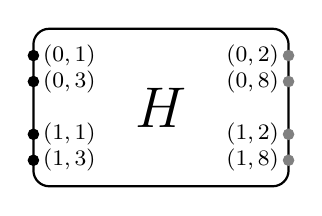
\begin{tikzpicture}
  \draw[rounded corners=2mm,thick] (0,0) rectangle (3.24 cm, 2cm);
  % Drawing the nodes 
 \foreach \y in {.33,.66,1.33,1.66}
{ 
 \foreach \x/\color in {0/black,3.24/gray}
{      
\draw[fill=\color,draw=\color] (\x cm, \y cm) circle (.66mm);   
}
}   
  % Labels   
\foreach \z in {0,1}
{    
\node[right] at (0,1.66-\z) {\footnotesize $(\z,1)$}; 
\node[right] at (0,1.33-\z) {\footnotesize $(\z,3)$};    
% Output nodes change for each type 
   \node[left] at (3.24,1.66-\z) {\footnotesize $(\z,2)$}; 
   \node[left] at (3.24,1.33-\z) {\footnotesize $(\z,8)$};  
}   
  % Type of Graph
  \node at (1.62,1) {\huge $H$};   
\end{tikzpicture} 
  \label{fig:diagram_elementH}  
} 
\qquad
\subfloat[][]{
%%%%%%%%% Hadamard * T %%%%%%%%%
  \tikzsetnextfilename{MP_diagram_elementHT}
  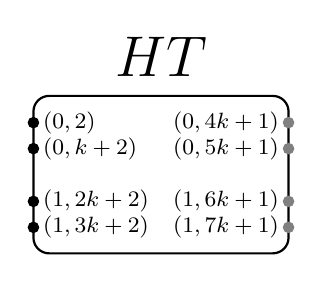
\begin{tikzpicture}
  \draw[rounded corners=2mm,thick] (0,0) rectangle (3.24 cm, 2cm);
  % Drawing the nodes   
\foreach \y in {.33,.66,1.33,1.66}
{  
\foreach \x/\color in {0/black,3.24/gray}
{     
\draw[fill=\color,draw=\color] (\x cm, \y cm) circle (.66mm);   
}
}     
% Labels  
\node[right] at (0,1.66) {\footnotesize $(0,2)$}; 
\node[right] at (0,.66) {\footnotesize $(1,2k+2)$}; 
\node[right] at (0,1.33) {\footnotesize $(0,k+2)$};
\node[right] at (0,.33) {\footnotesize $(1,3k+2)$};    
% Output nodes change for each type 
   \node[left] at (3.24,1.66) {\footnotesize $(0,4k+1)$}; 
   \node[left] at (3.24,1.33) {\footnotesize $(0,5k+1)$};
   \node[left] at (3.24,.66) {\footnotesize $(1,6k+1)$}; 
   \node[left] at (3.24,.33) {\footnotesize $(1,7k+1)$};  
 % Type of Graph  
\node at (1.62,2.5) {\huge $HT$}; 
 \end{tikzpicture}

  \label{fig:diagram_elementHT}
} 
\qquad 
\subfloat[][]
{
%%%%%%%%% Identity %%%%%%%%%
  \tikzsetnextfilename{MP_diagram_element1}
  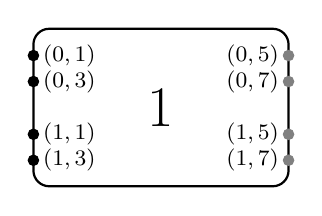
\begin{tikzpicture}
  \draw[rounded corners=2mm,thick] (0,0) rectangle (3.24 cm, 2cm);
  % Drawing the nodes  
\foreach \y in {.33,.66,1.33,1.66}
{   
\foreach \x/\color in {0/black,3.24/gray}
{     
\draw[fill=\color,draw=\color] (\x cm, \y cm) circle (.66mm);   
}
}    
 % Labels  
\foreach \z in {0,1}
{     
\node[right] at (0,1.66-\z) {\footnotesize $(\z,1)$};   
 \node[right] at (0,1.33-\z) {\footnotesize $(\z,3)$};    
% Output nodes change for each type   
 \node[left] at (3.24,1.66-\z) {\footnotesize $(\z,5)$};  
  \node[left] at (3.24,1.33-\z) {\footnotesize $(\z,7)$};   }    
 % Type of Graph  
\node at (1.62,1) {\huge $1$};  
\end{tikzpicture}  
  \label{fig:diagram_element1}
}
\caption[Diagram elements]{Diagram elements from which a gate diagram is constructed. Each diagram element is a schematic representation of the graph $g_{0}$ shown
in \fig{g_0}. 
\label{fig:diagram_elements}}
\end{figure}

Each diagram element corresponds to two copies of the graph $g_0$, along with self-loops and edges between the two copies.  The idea of these elements is to ensure that the ground state of the diagram element is closely related to that of the $g_0$ graph, but where almost all of the vertices of the diagram element has a self-loop.  The only vertices without such a self-loop are those corresponding to input and outputs of the diagram element, which will have a self-loop added to them in the final gate diagram.


Along these lines, each diagram element will be labeled by the unitary it computes, along with four numbers between zero and two, corresponding to the number of inputs ``nodes'' and output ``nodes'' for each logical state of the diagram.  Each such node will correspond to 16 vertices of the underlying graph representing one logical state and time of the two $g_0$ graphs.  These nodes are placed so that the minimal distance between two vertices in separate nodes will be at least $\dmax$.  

Explicitly, each diagram element will be labeled by a unitary $U\in \{\II, H, HT\}$, along with four integers $n_{0,\text{in}}$, $n_{0,\text{out}}$, $n_{1,\text{in}}$, and $n_{1,\text{out}}$, each between 0 and 2.  These numbers correspond to the number of nodes for each particular input or output.  We shall label such a diagram element a $U^{(n_{0,\text{in}},n_{1,\text{in}})}_{(n_{0,\text{out}},n_{1,\text{out}})}$ element.  The vertex set for the corresponding diagram element corresponds to two copies of $g_0$ (namely, $2\times 8k \times 8 \times 2$ vertices, labeled as $(z,t,j,d)$ for $z,d\in \FF_2$, $t\in [8k]$, and $j\in [8]$).  

For each node of the gate diagram, we will associate a time for which the underlying history state has computed the correct unitary.  Further, we will have these times each be a distance of at least $\dmax$ apart, to ensure that each node is at least a distance $\dmax$ apart.  Namely, for each logical input and output, we will associate two times:
\begin{itemize}
  \item $0$-input: $t_{0,1}^{\text{in}} = 2$ and $t_{0,2}^{\text{in}} = k+2$,
  \item $1$-input: $t_{1,1}^{\text{in}} = 2k+2$ and $t_{1,2}^{\text{in}} = 3k+2$,
  \item $0$-output: $t_{0,1}^{\text{out}} = 4k+\ell$ and $t_{0,2}^{\text{out}} = 5k+\ell$,
  \item $1$-output: $t_{1,1}^{\text{out}} = 4k+\ell$ and $t_{1,2}^{\text{out}} = 5k+\ell$,
\end{itemize}
where $\ell$ is $1$, $2$, or $3$, depending on whether the labeled unitary is $HT$, $\II$, or $H$, respectively.

For a given diagram element $U^{(n_{0,\text{in}},n_{1,\text{in}})}_{(n_{0,\text{out}},n_{1,\text{out}})}$, it will be useful to have defined the set of logical states and corresponding times explicitly used as input and output in the diagram element.  As such, let $T\subset \FF_2 \times [8k]$ be defined as
\begin{equation}
  T =\bigcup_{z\in \FF_2} \{(z, t_{z,j}^{\text{in}} ): j \leq n_{z,\text{in}}\} \cup \{(z, t_{z,j}^{\text{out}}) : j \leq n_{z,\text{out}}\},
\end{equation}
and note that $T$ contains those nodes (i.e., the sets of times and logical states) used as input and output for the given gate diagram, and that $|T|$ corresponds to the number of nodes in the diagram element.

With $T$ defined, the adjacency matrix for the corresponding diagram element $U^{(a,b)}_{(c,d)}$ will be
\begin{align}
  A\Big(G_U^{(a,b),(c,d)}\Big) &= A(g_0) \otimes \II_{2} + \sum_{(z,t)\notin T,j\in[8]} \ketbra{z,t,j}{z,t,j} \otimes \sum_{a,b\in \FF_2} \ketbra{a}{b} \\
   &= A(g_0)\otimes \II_2 + 2 \Pi_{\lnot T} \otimes \II_{8} \otimes \ketbra{+}{+}
\label{eq:diagram_element}
\end{align}
In particular, the graph for $G_U^{(a,b),(c,d)}$ will simply correspond to two copies of $g_0$, along with a projector onto the equal superposition between the two graphs for each vertex not used in a node of the diagram.

Because of the very similar form between $G_U^{(a,b),(c,d)}$ and $g_0$, their ground spaces and ground energies are closely related.  As the second term in \eq{diagram_element} is positive semi-definite, we have that the ground energy of $A(G_U^{(a,b),(c,d)})$ is at least that of $A(g_0)$. With more exact results, we have the following lemma:
\begin{lemma}
  Let $G_{U}^{(a,b),(c,d)}$ be the graph corresponding to a diagram element.  The ground space of $A(G_U^{(a,b),(c,d)})$ is
  \begin{equation}
    S = \spn\{ \ket{\psi_{z,a},-} : z,a\in \FF_2\}.
  \end{equation}
  \label{lem:diagram_element_ground}
\end{lemma}
\begin{proof}
  Note that $A(G_U^{(a,b),(c,d)})$ commutes with $\II_{2}\otimes \II_{8k} \otimes \II_8 \otimes \ketbra{+}{+}$, and thus there exists an eigenbasis for the adjacency matrix in which each vector is of the form $\ket{\phi}\ket{+}$ or $\ket{\phi}\ket{-}$.   For states of this latter form, the second term in \eq{diagram_element} vanishes, so  $\ket{\psi,-}$ is in the ground space of $A(g_U^{(a,b),(c,d)})$ if and only if $\ket{\psi}$ is in the ground space of $A(g_0)$, and thus we have that $S$ is a subspace of the nullspace.
  
  Now let us examine $\ket{\alpha,+}$ for any state $\ket{\alpha}$.  Since the second term of \eq{diagram_element} is positive semi-definite, we have that the ground energy of $A(G_U^{(a,b),(c,d)})$ is at least $e_1$.  Hence, if $\ket{\alpha,+}$ is in the ground space, then 
\begin{equation}
  \bigbra{\alpha,+} A\big(G_U^{(a,b),(c,d)}\big) \bigket{\alpha,+} = e_1 = \bra{\alpha} A(g_0) \ket{\alpha}
\end{equation}
and thus 
\begin{equation}
  \bra{\alpha} \Pi_{\lnot S}\otimes \II_8 \ket{\alpha} = 0,
\end{equation}
with $\ket{\alpha}$ in the ground space of $A(g_0)$.
  
  However, note that for all diagram elements (and all $\dmax$), $(z,0)$ is not in $T$.  We then have that
  \begin{equation}
    \Pi_{\lnot S} \geq \II_2 \otimes \ketbra{0}{0} \otimes \II_8.
  \end{equation}
  As this operator is strictly positive when restricted to the ground space of $A(g_0)$,
  \begin{equation}
    \bra{\psi_{x,\gamma}} \II_2 \otimes \ketbra{0}{0} \otimes \II_8 \ket{\psi_{z,\delta}} = \frac{1}{8k} \delta_{\gamma,\delta} \delta_{x,z},
  \end{equation}
  we also have that  $\Pi_{\lnot S}$ is strictly positive when restricted to the ground space of $A(g_0)$, and thus $\ket{\alpha,+}$ is not in the ground space of $A(G_U^{(a,b),(c,d)})$.
  
  Putting this together, we have that the ground space of $A(G_U^{(a,b),(c,d)})$ is $S$, as claimed 
\end{proof}

With this bound on the form of the ground space of $A(G_U^{(a,b),(c,d)})$, we can then use our knowledge of the two-particle interaction Hamiltonian on $g_0$ to relate this to the two-particle interaction Hamiltonian on $G_U^{(a,b),(c,d)}$.    Namely, we show that since there does not exist a two-particle frustration-free state on $g_0$, there also does not exists a two-particle frustration-free state on $G_U^{(a,b),(c,d)}$.

\begin{lemma}
  If $\dmax >0$, then $\lambda_2^1(G_U^{(a,b),(c,d)}) > 0$ for all states.  If $\dmax = 0$, then when restricted to symmetric states, $\lambda_2^1(G_U^{(a,b),(c,d)}) > 0$.
  \label{lem:2particle_element_bound}
\end{lemma}
\begin{proof}
  Note that using \lem{diagram_element_ground}, the ground space of $A(G_U^{(a,b),(c,d)})$ is in one-to-one correspondence with the ground space of $A(g_0)$, by the transformation
  \begin{equation}
    \ket{\phi_{x,a},-} \leftrightarrow \ket{\phi_{x,a}}\label{eq:phi_copy_transform}.
  \end{equation}
  Namely, by attaching (or removing) a second register in the $\ket{-}$ state, corresponding to having equal and opposite amplitudes between the two copies of $g_0$ present in $G_U^{(a,b),(c,d)}$, we can transform between these two single-particle ground spaces.
  
  We will use this relation, along with the fact that $\lambda_2^1(g_0) > 0$ from \lem{2particle}, to show that $\lambda_2^1(G_U^{(a,b),(c,d)}) > 0$ with the same assumptions.

  Let us then look at any two-particle state that minimizes the movement term.  In particular, it takes the form
  \begin{equation}
    \ket{\overline{\phi}} = \sum_{\alpha,\beta,x,z\in \FF_2} Q_{\alpha,\beta}^{x,z} \ket{\psi_{x,\alpha},-}\ket{\psi_{z,\beta},-}.
  \end{equation}
  Additionally, let us define the related two-particle state on $g_0$ as
  \begin{equation}
     \ket{\phi} = \sum_{\alpha,\beta,x,z\in \FF_2} Q_{\alpha,\beta}^{x,z} \ket{\psi_{x,\alpha}}\ket{\psi_{z,\beta}}.
  \end{equation}
  
  We can then see what the expectation of the interaction term of the Hamiltonian is under the state $\ket{\overline{\phi}}$: 
  \begin{align}
    \bra{\overline{\phi}} H_\text{int} \ket{\overline{\phi}} &= \sum_{u,v\in V(G_U^{(a,b),(c,d)})} \bra{\overline{\phi}} U_{d(u,v)}(\hat{n}_u,\hat{n}_v) \ket{\overline{\phi}}\\
      &= \sum_{u,v\in V(g_0),d_1,d_2\in \FF_2} \bra{\overline{\phi}} U_{d((u,d_1),(v,d_2))}(\hat{n}_{(u,d_1)},\hat{n}_{(v,d_2)}) \ket{\overline{\phi}}\\
      &\geq \sum_{u,v\in V(g_0),d_1\in \FF_2} \bra{\overline{\phi}} U_{d(u,v)} (\hat{n}_{(u,d_1)},\hat{n}_{(v,d_1)}) \ket{\overline{\phi}}
  \end{align}
  where in the third line we only count the contributions to the interaction when both particles are in the same copy of $g_0$.  As the interaction is positive-semidefinite, this can only decrease the expectation.  
  
  Now, from the form of $\ket{\overline{\phi}}$, we have that for any two $u,v\in V(g_0)$ and either copy of $g_0$,
  \begin{align}
    &\bra{\overline{\phi}} U_{d(u,v)} (\hat{n}_{(u,d_1)},\hat{n}_{(v,d_1)}) \ket{\overline{\phi}} \nonumber\\
    &\quad = \sum_{\substack{x_1,x_2,z_1,z_2\in\FF_2\\\alpha_1,\alpha_2,\beta_1,\beta_2\in\FF_2}}
    (Q_{\alpha_1,\beta_1}^{x_1,z_1})^* Q_{\alpha_2,\beta_2}^{x_2,z_2} \bra{\overline{\psi_{x_1,\alpha_1}}}\bra{\overline{\psi_{z_1,\beta_1}}} U_{d(u,v)}(\hat{n}_{(u,d_1)},\hat{n}_{(v,d_1)}) \ket{\overline{\psi_{x_2,\alpha_2}}}\ket{\overline{\psi_{z_2,\beta_2}}}\\
    &\quad \geq \big|\braket{d_1}{-}\big|^4\sum_{\substack{x_1,x_2,z_1,z_2\in\FF_2\\\alpha_1,\alpha_2,\beta_1,\beta_2\in\FF_2}}
    (Q_{\alpha_1,\beta_1}^{x_1,z_1})^* Q_{\alpha_2,\beta_2}^{x_2,z_2} \bra{\psi_{x_1,\alpha_1}}\bra{\psi_{z_1,\beta_2}} U_{d(u,v)}(\hat{n}_{u},\hat{n}_{v}) \ket{\psi_{x_2,\alpha_2}}\ket{\psi_{z_2,\beta_2}}\\
    &\quad = \frac{1}{4} \bra{\phi} U_{d(u,v)}(\hat{n}_u,\hat{n}_v)\ket{\phi}.
  \end{align}
  Hence, we have that
  \begin{align}
    \bra{\overline{\phi}} H_{\text{int}} \ket{\overline{\phi}}& \geq  \sum_{u,v\in V(g_0),d_1\in \FF_2} \bra{\overline{\phi}} U_{d(u,v)} (\hat{n}_{(u,d_1)},\hat{n}_{(v,d_1)}) \ket{\overline{\phi}}\\
     &\geq \frac{1}{4} \sum_{u,v\in V(g_0), d_1\in \FF_2} \bra{\phi} U_{d(u,v)}(\hat{n}_u,\hat{n}_v) \ket{\phi}\\
     &= \frac{1}{4} \sum_{d_1\in \FF_2} \bra{\phi} H_{\text{int}} \ket{\phi}\\
     &= \frac{1}{2} \bra{\phi} H_{\text{int}} \ket{\phi}\label{eq:g0_and_diagram_element_relation}.
  \end{align}
  Using \lem{2particle}, we have that \eq{g0_and_diagram_element_relation} is larger than zero for all states and interactions that satisfy the conditions of \lem{2particle}, and thus $\bra{\overline{\phi}} H_{\text{int}} \ket{\overline{\phi}} >0$.  As such, there does not exist a two-particle frustration-free state on the graph $G_U^{(a,b),(c,d)}$ under the same assumptions as for $g_0$.

\end{proof}

%%%%%%%%%%%%%%%%%%%%%%%%%%%%%%%%%%%%%
\subsubsection{Gate diagrams}\label{sec:gate_diagrams}

While the diagram elements do have nice properties, we will eventually want to construct larger graphs using the diagram elements as basic elements.  Further, as the diagram elements themselves are rather complicated graphs, it will be useful to have a diagrammatic construction for these graphs:  these shall be the gate diagrams.

The rules for constructing gate diagrams are simple. A gate diagram consists of some number $R \in \{1,2,\ldots\}$ of diagram elements, with self-loops attached to a subset $\mathcal{S}$ of the nodes and edges connecting a set $\mathcal{E}$ of pairs of nodes. A node may have a single edge or a single self-loop attached to it, but never more than one edge or self-loop and never both an edge and a self-loop. Each node in a gate diagram has a label $(q,z,t)$ where $q \in [R]$ indicates the diagram element it belongs to. An example is shown in \fig{simple_gate_diagram}.

Sometimes it is convenient to draw the input nodes on the right-hand side of a diagram element; e.g., in \fig{W_gadget} the node closest to the top left corner is labeled $(q,z,t)=(3,2,4k+3)$.

\begin{figure}
\centering 
\tikzsetnextfilename{MP_simple_gate_diagram}
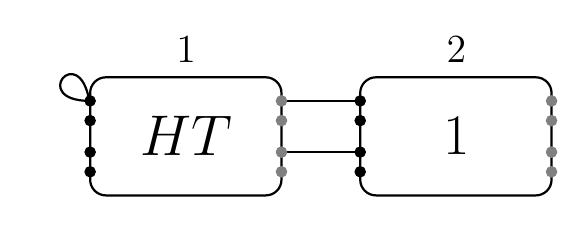
\begin{tikzpicture}
  % The connections 
 \foreach \y in {1.2,.55}
{   
 \draw[thick] (2.43,\y) -- (3.43,\y);  
}      
\draw[thick,looseness = 200] (0,1.2) to [out = 180, in = 100] (-.01,1.2);
  % The two rectangles 
 \foreach \offset/\unitary/\label in {0/HT/1,3.43/1/2}
{ 
 \begin{scope}[xshift=\offset cm] 
 \draw[rounded corners=2mm,thick] (0,0) rectangle (2.43cm,1.5 cm);
 \foreach \x /\color in {0/black,2.43/gray}
{     
\foreach \y in {1.2,.95,.55,.3}
{      
\draw[fill=\color,draw=\color] (\x cm, \y cm) circle (.66mm);  
  }
}    
\node at (1.22cm, .75cm) {\huge $\unitary$};   
 \node at (1.22cm, 1.85cm){\Large \label};  
\end{scope}
}    
\end{tikzpicture}
\caption[Diagram element example]{A gate diagram with two diagram elements labeled $q=1$ (left) and $q=2$ (right).
\label{fig:simple_gate_diagram}}
\end{figure}

To every gate diagram we associate a \emph{gate graph} $G$ with
vertex set 
\begin{equation}
\left\{ (q,z,t,j,d)\colon q\in[R],\, z,d\in\FF_2,\, t\in[8k],\, j\in [8]\right\} 
\end{equation}
and adjacency matrix 
\begin{align}
A(G) & =\sum_{q\in [R]} \ketbra{q}{q}\otimes A(G_q)+h_{\mathcal{S}}+h_{\mathcal{E}}\label{eq:adj_gate_graph}\\
A(G_q) &= A(G_{U_q}^{(a_q,b_q),(c_q,d_q)})\\
h_{\mathcal{S}} & =\sum_{\mathcal{S}}|q,z,t\rangle\langle q,z,t|\otimes\II_{8} \otimes \II_2\label{eq:h_loops}\\
h_{\mathcal{E}} & =\sum_{\mathcal{E}}\left(|q,z,t\rangle+|q^{\prime},z^{\prime},t^{\prime}\rangle\right)\left(\langle q,z,t|+\langle q^{\prime},z^{\prime},t^{\prime}|\right)\otimes\II_{8}\otimes \II_2.\label{eq:h_edges}
\end{align}
The sums in equations \eq{h_loops} and \eq{h_edges} run over the set of nodes with self-loops $(q,z,t)\in\mathcal{S}$ and the set of pairs of nodes connected by edges $\{(q,z,t),(q^{\prime},z^{\prime},t^{\prime})\}\in\mathcal{E}$, respectively. We see from the above expression that each self-loop in the gate diagram corresponds to $16$ self-loops in the graph $G$, and an edge in the gate diagram corresponds to $16$ edges and $32$ self-loops in $G$.  Note that we can determine the type of each diagram element from the gate diagram, as the implemented unitary and number of nodes is encoded in the diagram.

As a node in a gate graph never has more than one edge or self-loop attached to it, equations \eq{h_loops} and \eq{h_edges} are sums of orthogonal Hermitian operators.  Therefore 
\begin{align}
\left\Vert h_{\mathcal{S}}\right\Vert  & =\max_{\mathcal{S}}\left\Vert |q,z,t\rangle\langle q,z,t|\otimes\II_{j}\right\Vert =1\quad\text{if }\mathcal{S}\neq\emptyset\label{eq:h_S_bound}\\
\left\Vert h_{\mathcal{E}}\right\Vert  & =\max_{\mathcal{E}}\left\Vert \left(|q,z,t\rangle+|q^{\prime},z^{\prime},t^{\prime}\rangle\right)\left(\langle q,z,t|+\langle q^{\prime},z^{\prime},t^{\prime}|\right)\otimes\II_{j}\right\Vert =2\quad\text{if }\mathcal{E}\neq\emptyset\label{eq:h_E_bound}
\end{align}
for any gate graph. (Of course, this also shows that $\|{h_{\mathcal{S}^\prime}}\|=1$ and $\|{h_{\mathcal{E}^\prime}}\|=2$ for any nonempty subsets $\mathcal{S}^\prime\subseteq \mathcal{S}$ and $\mathcal{E}^\prime\subseteq \mathcal{E}$.)

Consider the adjacency matrix $A(G)$ of a gate graph $G$, and note (from equation \eq{adj_gate_graph} that its smallest eigenvalue $\mu(G)$ satisfies
\begin{equation}
\mu(G)\geq e_{1}
\end{equation}
since $h_{\mathcal{S}}$ and $h_{\mathcal{E}}$ are positive semidefinite and $A(G_{U}^{(a,b),(c,d)})$ has smallest eigenvalue $e_{1}$. In the special case where $\mu(G)=e_{1}$, we say $G$ is an $e_{1}$-gate graph.

\begin{definition}
An $e_{1}$-gate graph is a gate graph $G$ such that the smallest eigenvalue of its adjacency matrix is $e_{1}=-1-3\sqrt{2}$.
\end{definition}

When $G$ is an $e_{1}$-gate graph, a single-particle ground state $|\Gamma\rangle$ of $A(G)$ satisfies 
\begin{align}
\left(\sum_{q\in [R]} \ketbra{q}{q} \otimes A(G_q)\right)|\Gamma\rangle & =e_{1}|\Gamma\rangle\label{eq:Gamma_disc}\\
h_{\mathcal{S}}|\Gamma\rangle & =0\label{eq:h_s_0}\\
h_{\mathcal{E}}|\Gamma\rangle & =0.\label{eq:h_e_0}
\end{align}
Indeed, to show that a given gate graph $G$ is an $e_{1}$-gate graph, it suffices to find a state $|\Gamma\rangle$ satisfying these conditions. Note that equation \eq{Gamma_disc} implies that $|\Gamma\rangle$ can be written as a superposition of the states
\begin{equation}
  |\overline{\psi_{z,a}^{q}}\rangle=|q\rangle|\overline{\psi_{z,a}}\rangle,\quad
  z,a\in \FF_2, q\in[R]
\end{equation}
where $|\overline{\psi_{z,a}}\rangle$ is given by equations \eq{psi0m} and \eq{psi1m} under the transform of \eq{phi_copy_transform}. The coefficients in the superposition are then constrained by equations \eq{h_s_0} and \eq{h_e_0}.


\todo{fix frustration free stuff}

%
%\subsubsection{Frustration-free states for a given interaction range}
%

% 
%\begin{example}\label{ex:As-an-example}
%As an example, we show the gate graph in \fig{simple_gate_diagram} is an $e_{1}$-gate graph. As noted above, equation \eq{Gamma_disc} lets us restrict our attention to the space spanned by the eight states $|\psi_{z,a}^{q}\rangle$ with $z,a\in \{0,1\}$ and $q\in \{1,2\}$. In this basis, the operators $h_{\mathcal{S}}$ and $h_{\mathcal{E}}$ only have nonzero matrix elements between states with the same value of $a\in\{0,1\}$. We therefore solve for the $e_{1}$ energy ground states with $a=0$ and those with $a=1$ separately. Consider a ground state of the form
%\begin{equation}
%\left(\tau_{1}|\psi_{0,a}^{1}\rangle+\nu_{1}|\psi_{1,a}^{1}\rangle\right)+\left(\tau_{2}|\psi_{0,a}^{2}\rangle+\nu_{2}|\psi_{1,a}^{2}\rangle\right)
%\end{equation}
%and note that in this case \eq{h_s_0} implies $\tau_{1}=0$. Equation \eq{h_e_0} gives
%\begin{equation}
%\begin{pmatrix}
%\tau_{2}\\
%\nu_{2}
%\end{pmatrix}=\begin{cases}
%HT\begin{pmatrix}
%-\tau_{1}\\
%-\nu_{1}
%\end{pmatrix} & a=0\\
%(HT)^{*}\begin{pmatrix}
%-\tau_{1}\\
%-\nu_{1}
%\end{pmatrix} & a=1.
%\end{cases}
%\end{equation}
%We find two orthogonal $e_{1}$-energy states, which are (up to normalization)
%\begin{align}
%|\psi_{1,0}^{1}\rangle-\frac{e^{i\frac{\pi}{4}}}{\sqrt{2}}\left(|\psi_{0,0}^{2}\rangle-|\psi_{1,0}^{2}\rangle\right)\label{eq:example_ffstate_1}\\
%|\psi_{1,1}^{1}\rangle-\frac{e^{-i\frac{\pi}{4}}}{\sqrt{2}}\left(|\psi_{0,1}^{2}\rangle-|\psi_{1,1}^{2}\rangle\right) & .\label{eq:example_ffstate_2}
%\end{align}
%We interpret each of these states as encoding a qubit that is transformed at each set of input/output nodes in the gate diagram in \fig{simple_gate_diagram}. The encoded qubit begins on the input nodes of the first diagram element in the state 
%\begin{equation}
%\begin{pmatrix}
%\tau_{1}\\
%\nu_{1}
%\end{pmatrix}=\begin{pmatrix}
%0\\
%1
%\end{pmatrix}
%\end{equation}
%because the self-loop penalizes the basis vectors $|\psi_{0,a}^{1}\rangle$. On the output nodes of diagram element $1$, the encoded qubit is in the state where either $HT$ (if $a=0$) or its complex conjugate (if $a=1$) has been applied. The edges in the gate diagram ensure that the encoded qubit on the input nodes of diagram element 2 is minus the state on the output nodes of diagram element $1$.
%\end{example}
%
%In this example, each single-particle ground state encodes a single-qubit computation. Later we show how $N$-particle frustration-free states on $e_{1}$-gate graphs can encode computations on $N$ qubits. Recall from \defn{FF_states} that a state $|\Gamma\rangle\in\mathcal{Z}_{N}(G)$ is said to be frustration free iff $H(G,N)|\Gamma\rangle=0.$ Note that $H(G,N)\geq0$, so an $N$-particle frustration-free state is necessarily a ground state. Putting this together with \lem{increase_part_number}, we see that the existence of an $N$-particle frustration-free state implies
%\begin{equation}
%\lambda_{N}^{1}(G)=\lambda_{N-1}^{1}(G)=\ldots=\lambda_{1}^{1}(G)=0,
%\end{equation}
%i.e., there are $N^{\prime}$-particle frustration-free states for all $N^{\prime}\leq N$. 
%
%
%
%
%We now characterize the space of $N$-particle frustration-free states on an $e_{1}$-gate graph $G$. Define the subspace $\mathcal{I}(G,N)\subset\mathcal{Z}_{N}(G)$ where each particle is in a ground state of $A(g_{0})$ and no two particles are located within the same diagram element: 
%\begin{equation}
%  \mathcal{I}(G,N)=\spn\{
%  \Sym(|\psi_{z_{1},a_{1}}^{q_{1}}\rangle
%  % |\psi_{z_{2},a_{2}}^{q_{2}}\rangle
%  \ldots|\psi_{z_{N},a_{N}}^{q_{N}}\rangle)\colon 
%  z_{i},a_{i}\in\{0,1\},\; q_{i}\in[R],\; 
%  q_{i}\neq q_{j}\;\text{whenever}\; i\neq j\}.\label{eq:Ign}
%\end{equation}
%
%\begin{lemma}\label{lem:FF_characterization}
%Let $G$ be an $e_{1}$-gate graph. A state $|\Gamma\rangle\in\mathcal{Z}_{N}(G)$ is frustration free if and only if 
%\begin{align}
%\left(A(G)-e_{1}\right)^{(w)}|\Gamma\rangle & =0\;\text{ for all }w\in[N]\label{eq:ff_condition1}\\
%|\Gamma\rangle & \in\mathcal{I}(G,N).\label{eq:ff_condition2}
%\end{align}
%\end{lemma}
%
%\begin{proof}
%First suppose that equations \eq{ff_condition1} and \eq{ff_condition2} hold. From \eq{ff_condition2} we see that $|\Gamma\rangle$ has no support on states where two or more particles are located at the same vertex. Hence 
%\begin{equation}
%\sum_{k\in V}\hat{n}_{k}\left(\hat{n}_{k}-1\right)|\Gamma\rangle=0.\label{eq:ff_condition3}
%\end{equation}
%Putting together equations \eq{ff_condition1} and \eq{ff_condition3}, we get 
%\begin{equation}
%H(G,N)|\Gamma\rangle=\left(H_{G}^{N}-Ne_{1}\right)|\Gamma\rangle=0,
%\end{equation}
%so $|\Gamma\rangle$ is frustration free.
%
%To complete the proof, we show that if $|\Gamma\rangle$ is frustration free, then conditions \eq{ff_condition1} and \eq{ff_condition2} hold. By definition, a frustration-free state $|\Gamma\rangle$ satisfies 
%\begin{equation}
%H(G,N)|\Gamma\rangle=\left(\sum_{w=1}^{N}\left(A(G)-e_{1}\right)^{(w)}+\sum_{k\in V}\hat{n}_{k}\left(\hat{n}_{k}-1\right)\right)|\Gamma\rangle=0.\label{eq:defn_frustr}
%\end{equation}
%Since both terms in the large parentheses are positive semidefinite, they must both annihilate $|\Gamma\rangle$ (similarly, each term in the first summation must be zero). Hence equation \eq{ff_condition1} holds. Let $G_{\mathrm{rem}}$ be the graph obtained from $G$ by removing all of the edges and self-loops in the gate diagram of $G$. In other words,
%\begin{equation}
%A(G_{\mathrm{rem}})=\sum_{q=1}^{R}|q\rangle\langle q|\otimes A(g_{0})=\II\otimes A(g_{0}).
%\end{equation}
%Noting that 
%\begin{equation}
%H(G,N)\geq H(G_{\mathrm{rem}},N)\geq0,
%\end{equation}
%we see that equation \eq{defn_frustr} also implies 
%\begin{equation}
%H(G_{\mathrm{rem}},N)|\Gamma\rangle=0.\label{eq:Grem_gamma}
%\end{equation}
%Since each of the $R$ components of $G_{\mathrm{rem}}$ is an identical copy of $g_{0}$, the eigenvalues and eigenvectors of $H(G_{\mathrm{rem}},N)$ are characterized by \lem{BH_disconnected_graphs} (along with knowledge of the eigenvalues and eigenvectors of $g_{0}$). By \lem{2particle} and \lem{increase_part_number}, no component has a two- (or more) particle frustration-free state. Combining these two facts, we see that in an $N$-particle frustration-free state, every component of $G_{\mathrm{rem}}$ must contain either $0$ or $1$ particles, and the nullspace of $H(G_{\mathrm{rem}},N)$ is the space $\mathcal{I}(G,N).$ From equation \eq{Grem_gamma} we get $|\Gamma\rangle\in\mathcal{I}(G,N)$.
%\end{proof}
%
%Note that if $\mathcal{I}(G,N)$ is empty then \lem{FF_characterization} says that $G$ has no $N$-particle frustration-free states. For example, this holds for any $e_{1}$-gate graph $G$ whose gate diagram has $R<N$ diagram elements.
%
%A useful consequence of \lem{FF_characterization} is the fact that every $k$-particle reduced density matrix of an $N$-particle frustration-free state $|\Gamma\rangle$ on an $e_{1}$-gate graph $G$ (with $k\leq N$) has all of its support on $k$-particle frustration-free states. To see this, note that for any partition of the $N$ registers into subsets $A$ (of size $k$) and $B$ (of size $N-k$), we have
%\begin{equation}
%\mathcal{I}(G,N)\subseteq\mathcal{I}(G,k)_{A}\otimes\mathcal{Z}_{N-k}(G)_{B}.
%\end{equation}
%Thus, if condition \eq{ff_condition2} holds, then all $k$-particle reduced density matrices of $|\Gamma\rangle$ are contained in $\mathcal{I}(G,k)$. Furthermore, \eq{ff_condition1} is a statement about the single-particle reduced density matrices, so it also holds for each $k$-particle reduced density matrix. From this we see that each reduced density matrix of $|\Gamma\rangle$ is frustration free.


\subsection{Gadgets}\label{sec:gadgets}

\todo{rewrite this, removing the examples stuff}

In \ex{As-an-example} we saw how a single-particle ground state can encode a single-qubit computation. In this Section we see how a two-particle frustration-free state on a suitably designed $e_{1}$-gate graph can encode a two-qubit computation. We design specific $e_{1}$-gate graphs (called \emph{gadgets}) that we use in \sec{From-circuits-to} to prove that these ground state problems for the MPQW are QMA-hard. For each gate graph we discuss, we show that the smallest eigenvalue of its adjacency matrix is $e_{1}$ and we solve for all of the frustration-free states.

We first design a gate graph where, in any two-particle frustration-free state, the locations of the particles are synchronized.  We then design gadgets for two-qubit gates using four move-together gadgets, one for each two-qubit computational basis state. Finally, we describe a small modification of a two-qubit gate gadget called the ``boundary gadget.''

In important piece of these gadgets will be the inclusion of $\II_{(1,0)}^{(1,0)}$ diagram elements to separate the locations of particles.  With these separations, we will only ever need to analyze the case when particles occupy the same diagram element, as these identity elements ensure that for the states that we care about, particles are always located at a distance more than $\dmax$.

\subsubsection{The move-together gadget}



The gate diagram for the \emph{move-together gadget} is shown in \fig{W_gadget}. Using equation \eq{adj_gate_graph}, we write the adjacency matrix of the corresponding gate graph $G_W$ as 
\begin{equation}
A(G_W)=\sum_{q=1}^{14}|q\rangle\langle q|\otimes A(G_q)+h_{\mathcal{E}}\label{eq:move_together_adj}
\end{equation}
where
\begin{equation}
  G_q = \begin{cases}
    G_H^{(2,2),(1,1)} & q \in \{1,2\}\\
    G_\II^{(1,1),(0,0)} & q\in \{3,4,5,6\}\\
    G_\II^{(1,0),(1,0)} & q > 6,
  \end{cases}
\end{equation}
$h_{\mathcal{E}}$ is given by \eq{h_edges}, $h_{\mathcal{S}}$ is given by \eq{h_loops},  $\mathcal{E}$ is the set of edges in the gate diagram, and $\mathcal{S}$ is the set of self-loops in the diagram.

\begin{figure}
\centering 
\subfloat[][]{
\tikzsetnextfilename{MP_W_gadget}
\begin{tikzpicture}[scale=1]


% Left Connections between 1  and identity seperators
\foreach \l        /\r in {
	      3.24  / 3.525,
	      2.62  / 1.325,
	      1.04  / 2.425,
	      0.42  / 0.225
              } 
{   
 \draw[looseness=.66,line width=4pt,color=white] (-2.5,\l) to [out=0,in=180] (-1.5,\r);
 \draw[looseness=.66] (-2.5,\l) to [out=0,in=180] (-1.5,\r); 
}

% Connections between H and identity seperators
\foreach \l        /\r in {
	      3.24  / 3.525,
	      2.62  / 2.425,
	      1.04  / 1.325,
	      0.42  / 0.225
              } 
{   
 \draw[looseness=.66,line width=4pt,color=white] (1.5,\l) to [out=0,in=180] (2,\r);
 \draw[looseness=.66] (1.5,\l) to [out=0,in=180] (2,\r); 
 \draw[looseness=.66,line width=4pt,color=white] (0,\l) to [out=180,in=0] (-0.5,\r);
 \draw[looseness=.66] (0,\l) to [out=180,in=0] (-0.5,\r); 
}

% Right Connections between 1  and identity seperators
\foreach \l        /\r in {
	     3.525 / 1.04,
	     2.425 / 3.24,
	     1.325 / 2.62,
	     0.225 / 0.42
              } 
{   
 \draw[looseness=.66,line width=4pt,color=white] (3,\l) to [out=0,in=180] (4,\r);
 \draw[looseness=.66] (3,\l) to [out=0,in=180] (4,\r); 
}

% The two \II_{0,0}^{1,1} elements on the left

\foreach \yshift /\label in {0 / 4, 2.2 / 3} {
\begin{scope}[yshift=\yshift cm, xshift = - 4cm]
  \draw[rounded corners=0.75mm,thick] (0,0) rectangle (1.5 cm, 1.25cm);
  \node at (.75,.625) {\huge$\II$};   
  \node at (.75,1.5) {\large\label};
  \foreach \y in {1.04, .42} {
    \draw[fill = black, draw = black] (1.5 cm, \y cm) circle (.66mm);
  }  
\end{scope}
}

%  The Two H_{1,1}^{2,2} elements in the center

\foreach \yshift /\label in {0 / 2, 2.2 / 1} {
\begin{scope}[yshift=\yshift cm]
  \draw[rounded corners=0.75mm,thick] (0,0) rectangle (1.5 cm, 1.25cm);
  \node at (.75,.625) {\huge$H$};   
  \node at (.75,1.5) {\large\label};
  \foreach \y in {.21,.42,.83,1.04}{   
    \draw[fill=black,draw=black] (0 cm, \y cm) circle (.66mm);
  }
  \foreach \y in {1.04, .42} {
    \draw[fill = gray, draw = gray] (1.5 cm, \y cm) circle (.66mm);
  }  
\end{scope}
}

% The two \II_{0,0}^{1,1} elements on the right

\foreach \yshift /\label in {0 / 6, 2.2 / 5} {
\begin{scope}[yshift=\yshift cm, xshift = 4cm]
  \draw[rounded corners=0.75mm,thick] (0,0) rectangle (1.5 cm, 1.25cm);
  \node at (.75,.625) {\huge$\II$};   
  \node at (.75,1.5) {\large\label};
  \foreach \y in {1.04, .42} {
    \draw[fill = black, draw = black] (0 cm, \y cm) circle (.66mm);
  }  
\end{scope}
}



% Identity elements splitting the other six unitaries

\setcounter{mycount}{7}
\foreach \xshift in {-1.5,  2}
{
\foreach \yshift in {3.075,1.975,0.875,-0.225}{

\begin{scope}[shift = {(\xshift,\yshift)}]
  \draw[rounded corners = 0.75mm,thick] (0,0) rectangle (1 cm, .6cm);
  \node at (.5cm , .3 cm) {$\II$};
  \node at (.5cm , .8 cm) {$\arabic{mycount}$};
  \stepcounter{mycount}
  \draw[fill = black, draw=black] (0 cm, .15 cm) circle (.66mm);
  \draw[fill = black, draw=black] (0 cm, .45 cm) circle (.66mm);
  \draw[fill = gray,  draw =gray ] (1 cm, .45 cm) circle (.66mm);  
  
  % Self-loops on the second input node
  \draw[looseness=50,draw = black] (0cm, .14 cm) to [out = 210, in = 150] (0cm, .16cm);
\end{scope}
}}


\node at (0.23,3.03) {$\alpha$};
\node at (0.23,2.41) {$\beta$};
\node at (0.23,0.83) {$\delta$};
\node at (0.23,0.21) {$\gamma$};


\end{tikzpicture}

\label{fig:W_gadget_gate_diagram}}
\hspace{1cm}
\subfloat[][]{
\tikzsetnextfilename{MP_W_gadget_schematic}
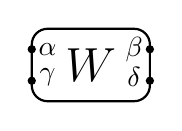
\begin{tikzpicture}

  \draw[rounded corners=2mm,thick] (0,-.46) rectangle (1.5cm,.46cm); 
    \node at (.75,0) {\LARGE $W$};
  \foreach \x/\y  in {0,1.5}
{  
\foreach \y in {-.2,.2}
{    
\draw[fill=black] (\x,\y) circle (.45mm);  
}
}      
\node at (.2,.2) {$\alpha$};  
\node at (.2,-.15) {$\gamma$}; 
 \node at (1.3,.2) {$\beta$}; 
 \node at (1.3,-.15) {$\delta$}; 

  
 \end{tikzpicture}
\label{fig:W_gadget_gate_schematic}}
\caption[Move-together gadget]{\subfig{W_gadget_gate_diagram} The gate diagram for the move-together gadget.  Note the four labeled nodes, $\alpha$, $\beta$, $\gamma$, and $\delta$, which have no attached edges.  \subfig{W_gadget_gate_schematic} A schematic representation for a move-together gadget, with the four labeled nodes corresponding to the four labeled nodes of \subfig{W_gadget_gate_diagram}. \label{fig:W_gadget}} 
\end{figure}

We begin by solving for the single-particle ground states, i.e., the eigenvectors of \eq{move_together_adj} with eigenvalue $e_{1}=-1-3\sqrt{2}$.  Note that we can solve for the states with $a=0$ and $a=1$ separately, since
\begin{equation}
  \langle\psi_{x,1}^{j}|h_{\mathcal{E}}|\psi_{z,0}^{i}\rangle=0
\end{equation}
for all $i,j\in[14]$ and $x,z\in \FF_2$. We write a single-particle ground state as
\begin{equation}
  \sum_{i=1}^{14}\left(\tau_{i}|\psi_{0,a}^{i}\rangle+\nu_{i}|\psi_{1,a}^{i}\rangle\right)
\end{equation}
and solve for the coefficients $\tau_{i}$ and $\nu_{i}$ using equation \eq{h_e_0}.  Enforcing \eq{h_s_0} gives us that $\nu_i = 0$ for all $i>6$. Enforcing \eq{h_e_0} gives sixteen equations, one for each edge in the gate diagram:
\begin{align}
  \tau_{3}&=-\tau_{7} & 
  \tau_{7}&= - \tau_{1}&
  \frac{1}{\sqrt{2}}(\tau_{1}+\nu_{1})&=-\tau_{11}&
  \tau_{11} &= -\tau_{6} \\
  \nu_{3} &= -\tau_{9}&
  \tau_{9} &= -\tau_{2} &
  \frac{1}{\sqrt{2}}(\tau_{2}+\nu_{2})&=-\tau_{13}&
  \tau_{13} &= - \nu_{5}\\
  \tau_{4}&=-\tau_{8} & 
  \tau_{8}&=-\nu_{1} &
  \frac{1}{\sqrt{2}}(\tau_{1}-\nu_{1})&=-\tau_{12} &
  \tau_{12} &= - \tau_{5}\\
  \nu_{3}&=-\tau_{10} & 
  \tau_{10} &= - \nu_{2} &
  \frac{1}{\sqrt{2}}(\tau_{2}-\nu_{2})&=-\tau_{14}&
  \tau_{14} &= - \nu_{6}  .
\end{align}
Similarly, enforcing \eq{h_s_0} gives eight equations, namely that $\nu_q = 0$ for $q>6$.  There are four linearly independent solutions to this set of equations, given by 
\begin{align}
  \text{\emph{Solution 1:}} && 
    \tau_{1} = \tau_{3} = -\tau_{7} &=1 & 
    \tau_{5} =  \tau_{6} = -\tau_{11} = - \tau_{12} &=\frac{1}{\sqrt{2}} &&
    \text{all other coefficients }0 \\
  \text{\emph{Solution 2:}} && 
    \nu_{1} = \tau_{4} = -\tau_{8} &=1 &
    -\tau_{5} =  \tau_{6} = -\tau_{11} = \tau_{12} &= \frac{1}{\sqrt{2}} &&
    \text{all other coefficients }0 \\
  \text{\emph{Solution 3:}} && 
    \nu_{2} = \nu_{4} = -\tau_{10} &= 1 &
    \nu_{5} = -\nu_{6} = -\tau_{13} = \tau_{14} &= \frac{1}{\sqrt{2}} &&
    \text{all other coefficients }0 \\
  \text{\emph{Solution 4:}} && 
    \tau_{2} =  \nu_{3} = -\tau_{9} &= 1 &
    \nu_{5} =  \nu_{6} = -\tau_{13} = -\tau_{14} &=\frac{1}{\sqrt{2}} &&
    \text{all other coefficients }0.
\end{align}
For each of these solutions, and for each $a\in\{0,1\}$, we find a single-particle state with energy $e_1$. This result is summarized in the following Lemma.

\begin{lemma}
$G_{W}$ is an $e_{1}$-gate graph. A basis for the eigenspace
of $A(G_{W})$ with eigenvalue $e_1$ is 
\begin{align}
  \ket{\chi_{1,a}} & =\frac{1}{\sqrt{5}}\big(\ket{\psi_{0,a}^{1}} + \ket{\psi_{0,a}^3} - \ket{\psi_{0,a}^7}\big) 
    +\frac{1}{\sqrt{10}}\big(\ket{\psi_{0,a}^{5}} + \ket{\psi_{0,a}^6} - \ket{\psi_{0,a}^{11}} - \ket{\psi_{0,a}^{12}}\big)\label{eq:chi_alpha}\\
  |\chi_{2,a}\rangle & =\frac{1}{\sqrt{5}}\big(\ket{\psi_{1,a}^{1}} + \ket{\psi_{0,a}^4} - \ket{\psi_{0,a}^8}\big) 
    +\frac{1}{\sqrt{10}}\big(-\ket{\psi_{0,a}^{5}} + \ket{\psi_{0,a}^6} - \ket{\psi_{0,a}^{11}} + \ket{\psi_{0,a}^{12}}\big)\label{eq:chi_beta}\\
  |\chi_{3,a}\rangle & =\frac{1}{\sqrt{5}}\big(\ket{\psi_{1,a}^{2}} + \ket{\psi_{1,a}^4} - \ket{\psi_{0,a}^{10}}\big) 
    +\frac{1}{\sqrt{10}}\big(\ket{\psi_{1,a}^{5}} - \ket{\psi_{1,a}^6} - \ket{\psi_{0,a}^{13}} + \ket{\psi_{0,a}^{14}}\big)\label{eq:chi_gamma}\\
|\chi_{4,a}\rangle & =\frac{1}{\sqrt{5}}\big(\ket{\psi_{0,a}^{2}} + \ket{\psi_{1,a}^3} - \ket{\psi_{0,a}^{9}}\big) 
    +\frac{1}{\sqrt{10}}\big(\ket{\psi_{1,a}^{5}} + \ket{\psi_{1,a}^6} - \ket{\psi_{0,a}^{13}} - \ket{\psi_{0,a}^{14}}\big)\label{eq:chi_delta}
\end{align}
where $a\in\FF_2$. 
\label{lem:w_gate_single_particle_basis}
\end{lemma}

In \fig{W_gadget} we have used a shorthand $\alpha,\beta,\gamma,\delta$ to identify four nodes of the move-together gadget; these are the nodes with labels $(q,z,t)=(1,0,2),(1,1,3k+2),(2,1,3k+2),(2,0,2)$, respectively. We view $\alpha$ and $\gamma$ as ``input'' nodes and $\beta$ and $\delta$ as ``output'' nodes for this gate diagram. It is natural to associate each single-particle state $|\chi_{i,a}\rangle$ with one of these four nodes.  We will also associate the set of 16 vertices represented by the node with the corresponding node, e.g.,
\begin{equation}
  S_{\alpha}=\left\{ (1,0,2,j,d)\colon j\in[8], d\in \FF_2\right\} .
\end{equation}
Looking at equation \eq{chi_alpha} (and perhaps referring back to equation \eq{psi0m}) we see that $|\chi_{1,a}\rangle$ has support on vertices in $S_{\alpha}$ but has no support on vertices in $S_{\beta}$, $S_{\gamma}$, or $S_{\delta}$. Looking at the picture on the right-hand side of the equality sign in \fig{W_gadget}, we think of $|\chi_{1,a}\rangle$ as localized at the node $\alpha$, with no support on the other three nodes. The states $|\chi_{2,a}\rangle,|\chi_{3,a}\rangle,|\chi_{4,a}\rangle$ are similarly localized at nodes $\beta,\gamma,\delta$. We view $|\chi_{1,a}\rangle$ and $|\chi_{3,a}\rangle$ as input states and $|\chi_{2,a}\rangle$ and $|\chi_{4,a}\rangle$ as output states for the move-together gadget.

Now we turn our attention to the two-particle frustration-free states of the move-together gadget, i.e., the states $|\Phi\rangle\in\HHH(G_{W})^{\otimes 2}$ in the nullspace of $H(G_W,2)$ (with the additional restriction to symmetric states if $\dmax = 0$). As $\lambda_2^1(G_{U}) >0$ for all $U$ from \lem{2particle_element_bound}, we have that any such state must take the form
\begin{equation}
|\Phi\rangle=\sum_{a,b \in \{0,1\},\,I,J \in [4]}C_{(I,a),(J,b)}|\chi_{I,a}\rangle|\chi_{J,b}\rangle\label{eq:chi_superposition}
\end{equation}
where 
\begin{equation}
\langle\psi_{z,a}^{q}|\langle\psi_{x,b}^{q}|\Phi\rangle=0\label{eq:frustration_free}
\end{equation}
for all $z,a,x,b\in\FF_2$ and $q\in[14]$, and where the coefficients are symmetric if $\dmax = 0$, i.e.,
\begin{equation}
C_{(I,a),(J,b)}=C_{(J,b),(I,a)},\label{eq:symmetric_coefs}.
\end{equation}  
Note that these conditions are only necessary, and not sufficient, for the state to be frustration free.  These conditions do not take into account the fact that the addition of edges might cause the distance of vertices to fall below $\dmax$, and thus add an interaction term between two occupied vertices.

However, in our construction of the $G_W$ gadget we placed the $H_{(1,0)}^{(1,1)}$ elements specifically to ensure that the two-particle states were separated by a distance of at least $2+ \dmax$.  Since each input/output node of a given diagram element is separated by a distance at least $\dmax$, if we can ensure that the state $\ket{\Phi}$ has no support on adjacent diagram elements, in addition to the other conditions in \eq{frustration_free}, then we can guarantee that $\ket{\Phi}$ is frustration-free.

The move-together gadget is designed so that each solution $|\Phi\rangle$ to these equations  is a superposition of a term where both particles are in input states and a term where both particles are in output states, with the intuition that particles move from input nodes to output nodes together. We now solve equations \eq{chi_superposition}--\eq{frustration_free} and prove the following.

\begin{lemma}
\label{lem:Wgadget_lemma}
A basis for the nullspace of $H(G_{W},2)$ is 
\begin{equation}
  |\Phi_{a,b}^{\pm}\rangle= \frac{1}{2} \big( |\chi_{1,a}\rangle|\chi_{3,b}\rangle \pm \ket{\chi_{3,b}}{\ket{\chi_{1,a}}} 
  + |\chi_{2,a}\rangle|\chi_{4,b}\rangle \pm \ket{\chi_{4,b}}\ket{\chi_{2,a}}\big),\quad a,b\in \FF_2\label{eq:phi_a1_a2}
\end{equation}
for $\dmax > 0$, and if $\dmax = 0$ a basis for the nullspace of $H(G_{W},2)$ when restricted to symmetric states is $\ket{\Phi_{a,b}^+}$ for $a,b\in \FF_2$.  

There are no $N$-particle frustration-free states on $G_{W}$ for $N\geq3$ for any $\dmax$ (with a restriction to symmetric states for $\dmax = 0$), i.e.,
\begin{equation}
\lambda_{N}^{1}(G_{W})>0\quad\text{for }N\geq3.
\end{equation}
\end{lemma}

\begin{proof}
The states $|\Phi_{a,b}^{\pm}\rangle$ manifestly satisfy equations \eq{chi_superposition}, and one can directly verify that they also satisfy \eq{frustration_free} (the nontrivial cases to check are for $q=5$, $q=6$, and $q>10$).  Additionally, one can also directly verify that $\ket{\Phi_{a,b}^{\pm}}$ has no support on states for which the two particles are located on adjacent diagram elements, and thus the state is in the ground space of the interaction Hamiltonian.

To complete the proof that \eq{phi_a1_a2} is a basis for the nullspace of $H(G_W,2)$, we will show that any state satisfying the conditions \eq{chi_superposition} and \eq{frustration_free} must be a linear combination of these four states.  Assuming that the state satisfies \eq{chi_superposition}, applying equation \eq{frustration_free} to the first $4$ diagram elements gives
\begin{align}
\langle\psi_{0,a}^{1}|\langle\psi_{0,b}^{1}|\Phi\rangle & =\frac{1}{5} C_{(1,a),(1,b)}=0 &
\langle\psi_{1,a}^{1}|\langle\psi_{1,b}^{1}|\Phi\rangle & =\frac{1}{5} C_{(2,a),(2,b)}=0\\
\langle\psi_{1,a}^{2}|\langle\psi_{1,b}^{2}|\Phi\rangle & =\frac{1}{5} C_{(3,a),(3,b)}=0 &
\langle\psi_{0,a}^{2}|\langle\psi_{0,b}^{2}|\Phi\rangle & =\frac{1}{5} C_{(4,a),(4,b)}=0\\
\langle\psi_{0,a}^{1}|\langle\psi_{1,b}^{1}|\Phi\rangle & =\frac{1}{5} C_{(1,a),(2,b)}=0 &
\langle\psi_{0,a}^{2}|\langle\psi_{1,b}^{2}|\Phi\rangle & =\frac{1}{5} C_{(4,a),(3,b)}=0\\
\langle\psi_{1,a}^{1}|\langle\psi_{0,b}^{1}|\Phi\rangle & =\frac{1}{5} C_{(2,a),(1,b)}=0 &
\langle\psi_{1,a}^{2}|\langle\psi_{0,b}^{2}|\Phi\rangle & =\frac{1}{5} C_{(3,a),(4,b)}=0\\
\langle\psi_{0,a}^{3}|\langle\psi_{1,b}^{3}|\Phi\rangle & =\frac{1}{5} C_{(1,a),(4,b)}=0 &
\langle\psi_{0,a}^{4}|\langle\psi_{1,b}^{4}|\Phi\rangle & =\frac{1}{5} C_{(2,a),(3,b)}=0\\
\langle\psi_{1,a}^{3}|\langle\psi_{0,b}^{3}|\Phi\rangle & =\frac{1}{5} C_{(4,a),(1,b)}=0 &
\langle\psi_{1,a}^{4}|\langle\psi_{0,b}^{4}|\Phi\rangle & =\frac{1}{5} C_{(3,a),(2,b)}=0
\end{align}
for all $a,b\in \{0,1\}$. Using the fact that all of these coefficients are zero, we can then see that
\begin{align}
|\Phi\rangle=\sum_{\substack{a,b\in\FF_2\\ j\in [4]}}C_{(j,a),(j+2,b)}|\chi_{j,a}\rangle|\chi_{j+2,b}\rangle.
\end{align}
Finally, applying equation \eq{frustration_free} to diagram $6$ gives
\begin{align}
\langle\psi_{0,a}^{6}|\langle\psi_{1,b}^{6}|\Phi\rangle&=\frac{1}{6}C_{(2,a),(4,b)}-\frac{1}{6}C_{(1,a),(3,b)}=0\\
\langle\psi_{1,a}^{6}|\langle\psi_{0,b}^{6}|\Phi\rangle&=\frac{1}{6}C_{(4,a),(2,b)}-\frac{1}{6}C_{(3,a),(1,b)}=0.
\end{align}
Hence
\begin{equation}
|\Phi\rangle=\sum_{\substack{a,b\in\FF_2\\j\in[4]}}C_{(j,a),(j+2,b)}\big(|\chi_{j,a}\rangle|\chi_{j+2,b}\rangle+|\chi_{j+1,a}\rangle|\chi_{j+3,b}\rangle\big),
\end{equation}
which is a superposition of the states $|\Phi_{a,b}^\pm\rangle.$ 

Note that the above analysis holds completely if we restrict ourselves to symmetric states, and thus if $\dmax = 0$, we end up with the same results except that we only care about the states $\ket{\Phi_{a,b}^+}$, as they span the symmetric nullspace.

Finally, we prove that there are no frustration-free ground states of the Bose-Hubbard model on $G_{W}$ with more than two particles. By \lem{increase_part_number},
it suffices to prove that there are no frustration-free three-particle states.

Suppose (for a contradiction) that $|\Gamma\rangle\in\mathcal{H}(G_{W})^{\otimes 3}$ is a normalized three-particle frustration-free state. Write 
\begin{equation}
|\Gamma\rangle=\sum D_{(i,a),(j,b),(k,c)}|\chi_{i,a}\rangle|\chi_{j,b}\rangle|\chi_{k,c}\rangle.
\end{equation}
Note that each reduced density matrix of $|\Gamma\rangle$ on two of the three subsystems must have all of its support on two-particle frustration-free states (see the remark following \lem{FF_characterization}), i.e., on the states $|\Phi_{a,b}\rangle$. Using this fact for the subsystem consisting of the first two particles, we see in particular that
\begin{equation}
(i,j)\notin\{(1,3),(3,1),(2,4),(4,2)\}\quad\Longrightarrow\quad D_{(i,a),(j,b),(k,c)}=0\label{eq:ij_constraint1}
\end{equation}
(since $|\Phi_{a_1,a_2}\rangle$ only has support on vectors $|\chi_{i,a}\rangle|\chi_{j,b}\rangle$ with $i,j\in \{(1,3),(3,1),(2,4),(4,2)\}$).

Using this fact for subsystems consisting of particles $2,3$ and $1,3$, respectively, gives 
\begin{align}
(j,k)\notin\{(1,3),(3,1),(2,4),(4,2)\}\quad\Longrightarrow\quad D_{(i,a),(j,b),(k,c)} & =0\label{eq:ij_constraint2}\\
(i,k)\notin\{(1,3),(3,1),(2,4),(4,2)\}\quad\Longrightarrow\quad D_{(i,a),(j,b),(k,c)} & =0.\label{eq:ij_constraint3}
\end{align}
Putting together equations \eq{ij_constraint1}, \eq{ij_constraint2}, and \eq{ij_constraint3}, we see that $|\Gamma\rangle=0$. This is a contradiction, so no three-particle frustration-free states exist.
\end{proof}

With this gadget allowing us to entangle the locations of particles, we will be able to create a pseudo-history state, in which time is encoded in the location of particles.  This is the large workhorse of the construction, as it allows us to understand the multi-particle ground space by understanding the simple two-particle ground states.


%%%%%%%%%%%%%%%

\subsubsection{Two-qubit unitary gadget}

We can now use the $W$-gadget as a building block to encode graphs with more interesting ground-state behavior.  In particular, we can use the $W$-gadget to force the two-particle state of a larger gadget to have entangled locations.  If we then place connections in a particular manner, we can use these guarantees to force the ground state to encode a computation corresponding to a permutation of the computational basis states (such as a controlled-not operation).  In particular, we will be to define a gate graph for each of the two-qubit unitaries
\begin{equation}
  \{\CNOT_{12}, \CNOT_{21}, \CNOT_{12}\left(H\otimes\II\right),
    \CNOT_{12}\left(HT\otimes\II\right)\}.
\end{equation}
Here $\CNOT_{12}$ is the standard controlled-not gate with the second qubit as a target, whereas $\CNOT_{21}$ has the first qubit as target.

We define the gate graphs by exhibiting their gate diagrams. For the three cases
\begin{equation}
  U=\CNOT_{12}(\tilde U\otimes\II)
\end{equation}
with $\tilde U\in\{\II,H,HT\}$, we associate $U$ with the gate diagram shown in \fig{GVucnotcomplete}. In \fig{GVucnot} we also indicate a shorthand used to represent this gate diagram. As one might expect, for the case $U=\CNOT_{21}$, we use the same gate diagram as for $U=\CNOT_{12}$; however, we use the slightly different shorthand shown in \fig{GVcnot}.

%%%%%%%%%%%%%%%%%%%%%%%%%%
\begin{figure}
\centering 
\subfloat[][]{
  \tikzsetnextfilename{MP_GVucnot_complete}
  \begin{tikzpicture}[yscale=1]
%\path[use as bounding box](-5.5,-3) rectangle (10,10.5); 


% Connections between the i/o unitaries and the identity separators
\foreach \xshift / \xscale in {-3.5/ 1, 5/-1}{
\foreach \yshift in {2.7, -1.7}{
\begin{scope}[shift = {(\xshift, \yshift)},xscale = \xscale]
  \draw[black, looseness = 1] (0,2.34) to [out=0, in = 180] (1,   3.75);
  \draw[black, looseness=1]   (0,2.13) to [out = 0, in = 180] (1, 2.65);
  \draw[black, looseness= 1]  (0,1.72) to [out = 0, in = 180] (1, 1.55);
  \draw[black, looseness = 1] (0,1.51) to [out = 0, in = 180] (1, 0.45);
\end{scope}
}}

% Left Connections between W and identity seperators
\foreach \l        /\r in {
	      6.45  /5.93,
	      5.35  /3.73,
	      4.25  /1.53,
	      3.15  /-0.67,
	      2.05  /5.51,
	      0.95  /1.11,
	      -0.15  /3.31,
	      -1.25  /-1.09
              } 
{   
 \draw[looseness=.66,line width=4pt,color=white] (-1.5,\l) to [out=0,in=180] (0,\r);
 \draw[looseness=.66] (-1.5,\l) to [out=0,in=180] (0,\r); 
}


% Right Connections between W and identity seperators
\foreach \l        /\r in {
              5.93  /6.45,
              5.51  /2.05,
              3.73  /5.35,
              3.31  /-0.15,
              1.53  /4.25,
              1.11  /-1.25,     
              -0.67/3.15,
              -1.09/0.95
              } 
{   
 \draw[looseness=.66,line width=4pt,color=white] (1.5,\l) to [out=0,in=180] (3,\r);
 \draw[looseness=.66] (1.5,\l) to [out=0,in=180] (3,\r); 
}


%  Edges between identity and preventing two-particle states

\draw[color = black]   (-2 cm, -3.4875 cm)  to[out = 180,in=0] (-3 cm, -3.65);
\draw[color = black] (-2 cm, -2.8625 cm)  to[out = 180,in=0] (-3 cm, -2.55);

\draw[color = black]   (3.5 cm, -3.4875 cm)  to[out = 0,in=180] (4.5 cm, -3.65);
\draw[color = black]   (3.5 cm, -2.8625 cm)  to[out = 0,in=180] (4.5 cm, -2.55);

\draw[color = black]  (-3cm, 8.85cm) to[out=0, in=180] (-2cm, 9.4375 cm);
\draw[color = black]  (4.5cm, 8.85cm) to[out=180, in=0] (3.5cm, 9.4375 cm);

\draw[color = black]  (-3cm, 7.75cm) to[out=0,in=180] (-0.5cm, 7.75cm) to[out=0, in=180] (2cm, 8.8125 cm);
\draw[color = white, line width=4pt]  (4.5cm, 7.75cm)  to[out=180, in=0] (2cm, 7.75cm) to[out=180, in=0](-0.5cm, 8.8125 cm);
\draw[color = black]  (4.5cm, 7.75cm)  to[out=180, in=0] (2cm, 7.75cm) to[out=180, in=0](-0.5cm, 8.8125 cm);

\draw[color = black] (-5cm , 4.83 cm) to[out=180, in=180] (-4cm, 8.85cm);
\draw[color = white, line width=4pt] (-5cm , 4.21 cm) to[out=180, in=180] (-4cm, 7.75cm);
\draw[color = black] (-5cm , 4.21 cm) to[out=180, in=180] (-4cm, 7.75cm);

\draw[color = black] (6.5cm , 4.83 cm) to[out=0, in=0] (5.5cm, 8.85cm);
\draw[color = white, line width=4pt] (6.5cm , 4.21 cm) to[out=0, in=0] (5.5cm, 7.75cm);
\draw[color = black] (6.5cm , 4.21 cm) to[out=0, in=0] (5.5cm, 7.75cm);

\draw[color = black] (-5cm , 0.43 cm) to[out=180, in=180] (-4cm, -2.55cm);
\draw[color = white, line width=4pt] (-5cm , -0.19 cm) to[out=180, in=180] (-4cm, -3.65cm);
\draw[color = black] (-5cm , -0.19 cm) to[out=180, in=180] (-4cm, -3.65cm);

\draw[color = black] (6.5cm , 0.43 cm) to[out=0, in=0] (5.5cm, -2.55cm);
\draw[color = white, line width=4pt] (6.5cm , -0.19 cm) to[out=0, in=0] (5.5cm, -3.65cm);
\draw[color = black] (6.5cm , -0.19 cm) to[out=0, in=0] (5.5cm, -3.65cm);



%  The four Unitaries used for input/output 
\foreach \xshift / \yshift /\xscale / \lab / \unitary in 
  {5  /-.4   /1  /4  /1,
   5  /4   /1  /2  /1,
  -5  /-.4   /1  /3  /1,
  -5 /4   /1  /1  /\tilde U
}
{ 
\begin{scope}[shift={(\xshift,\yshift)},xscale=\xscale]
  \draw[rounded corners=0.75mm,thick] (0,0) rectangle (1.5 cm, 1.25cm);
  \node at (.75,.625) {\huge$\unitary$};   
  \node at (.75,1.5) {\large\lab};
  \foreach \y in {.21,.42,.83,1.04}
	{   
		\foreach \x /\color in {0/black,1.5/gray}
			{    
				\draw[fill=\color,draw=\color] (\x cm, \y cm) circle (.66mm);  
			}
	} 
\end{scope}
}


% Identity elements splitting the four i/o unitaries from the W-gadgets

\setcounter{mycount}{9}
\foreach \xshift in { -2.5,  3}
{
\foreach \yshift in {6,4.9,3.8,...,-2}{

\begin{scope}[shift = {(\xshift,\yshift)}]
  \draw[rounded corners = 0.75mm,thick] (0,0) rectangle (1 cm, .6cm);
  \node at (.5cm , .3 cm) {$1$};
  \node at (.5cm , .8 cm) {$\arabic{mycount}$};
  \stepcounter{mycount}
  \draw[fill = black, draw=black] (0 cm, .15 cm) circle (.66mm);
  \draw[fill = black, draw=black] (0 cm, .45 cm) circle (.66mm);
  \draw[fill = gray,  draw =gray ] (1 cm, .45 cm) circle (.66mm);  
  
  % Self-loops on the second input node
  \draw[looseness=50,draw = black] (0cm, .14 cm) to [out = 210, in = 150] (0cm, .16cm);
\end{scope}
}}

% Identity operators preventing two-particle states

\draw[rounded corners=0.75mm,thick] (-2,8.5) rectangle (-0.5 cm, 9.75cm);
\node at (-1.25,9.125) {\huge$1$};   
\node at (-1.25,10) {\large$5$};
\draw[fill = black, draw = black] (-2 cm, 9.4375 cm) circle (.66mm);
\draw[fill = gray, draw = gray]    (-.5cm, 8.8125 cm) circle (.66mm);

\draw[rounded corners=0.75mm,thick] (2,8.5) rectangle (3.5 cm, 9.75cm);
\node at (2.75,9.125) {\huge$1$};   
\node at (2.75,10) {\large$6$};
\draw[fill = gray, draw = gray] (3.5 cm, 9.4375 cm) circle (.66mm);
\draw[fill = black, draw = black]    (2cm, 8.8125 cm) circle (.66mm);


% Identity operators preventing two-particle state scaling

\draw[rounded corners=0.75mm,thick] (-2,-3.8) rectangle (-0.5 cm, -2.55cm);
\node at (-1.25,-3.125) {\huge$1$};   
\node at (-1.25,-2.3) {\large$7$};
\draw[fill = black, draw = black] (-2 cm, -3.4875 cm) circle (.66mm);
\draw[fill = black, draw = black] (-2 cm, -2.8625 cm) circle (.66mm);

\draw[rounded corners=0.75mm,thick] (2,-3.8) rectangle (3.5 cm, -2.55cm);
\node at (2.75,-3.125) {\huge$1$};   
\node at (2.75,-2.3) {\large$8$};
\draw[fill = black, draw = black] (3.5 cm, -3.4875 cm) circle (.66mm);
\draw[fill = black, draw = black] (3.5 cm, -2.8625 cm) circle (.66mm);m);


% Identity elements separating  identity preventing unwanted two-particle states
\foreach \xshift in { -4,  4.5}
{
\foreach \yshift in {8.4,7.3,-3, -4.1}{

\begin{scope}[shift = {(\xshift,\yshift)}]
  \draw[rounded corners = 0.75mm,thick] (0,0) rectangle (1 cm, .6cm);
  \node at (.5cm , .3 cm) {$1$};
  \node at (.5cm , .8 cm) {$\arabic{mycount}$};
  \stepcounter{mycount}
  \draw[fill = black, draw=black] (0 cm, .15 cm) circle (.66mm);
  \draw[fill = black, draw=black] (0 cm, .45 cm) circle (.66mm);
  \draw[fill = gray,  draw =gray ] (1 cm, .45 cm) circle (.66mm);  
  
  % Self-loops on the second input node
  \draw[looseness=50,color = black] (0cm, .14 cm) to [out = 210, in = 150] (0cm, .16cm);
\end{scope}
}}




  % Each W Gadget
\foreach \yshift/\from in {-1.35/11,0.85 /10,3.05/01,5.25/00}
{ 
\begin{scope}[yshift=\yshift cm] 
 \draw[rounded corners=0.75mm,thick] (0,0) rectangle (1.5cm,.93cm); 
 \node at (.75,.465) {$W$};   
\node at (.75,1.2) {$\from$};
  \foreach \x/\color in {0/black,1.5/gray}
	{   
		\foreach \y in {0.26,.67}
		{   
			 \draw[fill=\color,draw=\color] (\x,\y) circle (.66mm); 
		 }
	}
\end{scope}
}

\node at (-5.25, 5.1) {\small$\alpha$};
\node at (-5.25, 4.5) {\small$\beta$};

\node at (-5.25, 0.6) {\small$\gamma$};
\node at (-5.25, 0)   {\small$\delta$};


\node at (6.75, 5.1) {\small$\epsilon$};
\node at (6.75, 4.5) {\small$\zeta$};

\node at (6.75, 0.6) {\small$\eta$};
\node at (6.75, 0)   {\small$\theta$};

\end{tikzpicture}
\label{fig:GVucnot_complete}
  \vspace{0.63cm}
  \label{fig:GVucnotcomplete}}\\
\subfloat[][]{
  \tikzsetnextfilename{MP_GVucnot}
  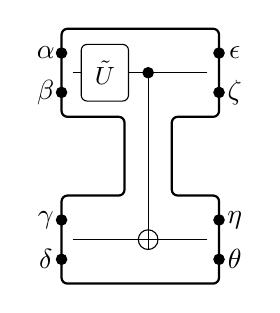
\begin{tikzpicture}[yscale=1]

 \begin{scope}[xscale=-1,xshift=-2cm]   
\draw[rounded corners = .75mm,thick] (0cm, -1.618 cm) -- (2 cm, -1.618 cm) -- (2cm, -.5 cm) -- (1.2cm, -.5 cm) -- (1.2 cm,.5cm) -- (2cm, .5cm) -- (2cm, 1.618cm) -- (0cm, 1.618cm) -- (0cm, .5cm) -- (.6cm, .5cm) -- (.6cm, -.5cm) -- (0cm, -.5cm) -- cycle; 
    \draw (.15cm, 1.06cm) -- (1.85cm, 1.06cm); 
 \draw (.15cm, -1.06cm) -- (1.85cm, -1.06cm);
  \draw (.9cm,1.06cm) -- (.9cm,-1.06cm);   
\draw[fill=black] (.9,1.06cm) circle (.66mm); 
 \draw (.9,-1.06cm) circle (1.25mm); 
 \draw (.9,-1.19cm) -- (.9,-.93cm);   
  \draw[rounded corners=.75mm,fill=white] (1.15cm, .7cm) rectangle (1.75cm, 1.42cm); 
 \node at (1.45cm, 1.06cm) {\small $\tilde U$}; 
 \end{scope}   


\node at ( -0.2,1.31) {$\alpha$};
 \draw[fill=black] (0,1.31) circle (.66mm);   

\node at ( -0.2,0.81) {$\beta$};
 \draw[fill=black] (0,0.81) circle (.66mm);   

\node at ( -0.2,-0.81) {$\gamma$};
 \draw[fill=black] (0,-0.81) circle (.66mm);   

\node at ( -0.2,-1.31) {$\delta$};
 \draw[fill=black] (0,-1.31) circle (.66mm);   

\node at (2.2,1.31) {$\epsilon$};
 \draw[fill=black] (2,1.31) circle (.66mm);   

\node at (2.2,0.81) {$\zeta$};
 \draw[fill=black] (2,0.81) circle (.66mm);   

\node at ( 2.2,-0.81) {$\eta$};
 \draw[fill=black] (2,-0.81) circle (.66mm);   

\node at ( 2.2,-1.31) {$\theta$};
 \draw[fill=black] (2,-1.31) circle (.66mm);   

\end{tikzpicture}
\label{fig:GVucnot}
  \vspace{0.63cm}
  \label{fig:GVucnot}}
\subfloat[][]{
  \tikzsetnextfilename{MP_GVcnot}
  
\begin{tikzpicture}[yscale= 1] 

  \setcounter{mycount}{`a} \begin{scope}[xshift = 7.2 cm,yshift = 3cm]   
     
\draw[rounded corners = .75mm,thick] (0cm, -1.618 cm) -- (2 cm, -1.618 cm) -- (2cm, -.5 cm) -- (1.2cm, -.5 cm) -- (1.2 cm,.5cm) -- (2cm, .5cm) -- (2cm, 1.618cm) -- (0cm, 1.618cm) -- (0cm, .5cm) -- (.6cm, .5cm) -- (.6cm, -.5cm) -- (0cm, -.5cm) -- cycle;      \draw (.15cm, 1.06cm) -- (1.85cm, 1.06cm);   \draw (.15cm, -1.06cm) -- (1.85cm, -1.06cm);   \draw (.9cm,1.06cm) -- (.9cm,-1.06cm);
 \draw[fill=black] (.9,-1.06cm) circle (.66mm);   \draw (.9,1.06cm) circle (1.25mm);   \draw (.9,1.19cm) -- (.9,.93cm); 


\node at ( -0.2,-0.81) {$\alpha$};
 \draw[fill=black] (0,-0.81) circle (.66mm);   

\node at ( -0.2,-1.31) {$\beta$};
 \draw[fill=black] (0,-1.31) circle (.66mm);   

\node at ( -0.2,1.31) {$\gamma$};
 \draw[fill=black] (0,1.31) circle (.66mm);   

\node at ( -0.2,0.81) {$\delta$};
 \draw[fill=black] (0,0.81) circle (.66mm);   

\node at ( 2.2,-0.81) {$\epsilon$};
 \draw[fill=black] (2,-0.81) circle (.66mm);   

\node at ( 2.2,-1.31) {$\zeta$};
 \draw[fill=black] (2,-1.31) circle (.66mm);   

\node at (2.2,1.31) {$\eta$};
 \draw[fill=black] (2,1.31) circle (.66mm);   

\node at (2.2,0.81) {$\theta$};
 \draw[fill=black] (2,0.81) circle (.66mm);   

\end{scope}
\end{tikzpicture}
  \label{fig:GVcnot}}
\caption[Two-qubit gadget]{\subfig{GVucnotcomplete} Gadget for the
 two-qubit unitary $U=\CNOT_{12}(\tilde U\otimes\II)$ with $\tilde U\in \{1,H,HT\}$. \subfig{GVucnot} A schematic encoding for $U=\CNOT_{12}(\tilde U\otimes \II)$, where the eight labeled nodes correspond to the eight labeled nodes of \subfig{GVucnotcomplete}.
\subfig{GVcnot} For the $U=\CNOT_{21}$ gate (first qubit is the target), we use the same gate graph as in \subfig{GVucnot} with $\tilde U=1$, but with a different location for the eight labeled nodes.}
\label{fig:GVcnot_tot}
\end{figure}

Roughly speaking, the two-qubit gate gadgets work as follows.  There are four move-together gadgets, one for each two-qubit basis state $|00\rangle, |01\rangle, |10\rangle, |11\rangle$. These enforce the constraint that two particles must move through the graph together, while their connections to the four diagram elements labeled $1,2,3,4$ ensure that most of the frustration-free two-particle states encode two-qubit computations, while the connections between diagram elements $1,2,3,4$ and $5,6,7,8$ ensure that the remaining frustration-free two-particle states are removed from the ground space.   The $24$ $\II_{(1,0)}^{(1,1)}$ diagram elements are simply used to separate the locations of the particles when more than one are located on the gadget, but can simply be thought of as a part of the connections between the other gadgets.

To describe the frustration-free states of the gate graph depicted in \fig{GVcnot_tot}, first recall the definition of the states $|\chi_{j,a}\rangle$ for $j\in [4]$  from equations \eq{chi_alpha}--\eq{chi_delta}. For each of the move-together gadgets $xy\in\{00,01,10,11\}$ in \fig{GVucnot}, write 
$
|\chi_{j,a}^{xy}\rangle
$
for the state $|\chi_{j,a}\rangle$ with support (only) on the gadget labeled $xy$. Additionally, write 
\begin{equation}
  U^a=\begin{cases}
    U & \text{ if }a=0\\
    \overline{U} & \text{ if }a=1
  \end{cases}
\end{equation}
and similarly for $\tilde U$.  This notation will help us to define the ground states of the resulting Hamiltonian, as the encoded computation will change depending on $\alpha$.



We now show that $G_{U}$ is an $e_{1}$-gate graph and solves for its frustration-free states.

\begin{lemma}\label{lem:2qub_gate}
Let $U=\CNOT_{12}(\tilde U\otimes\II)$ where $\tilde U\in\{\II,H,HT\}$. The corresponding gate graph $G_U$ is defined by its gate diagram shown in \fig{GVucnotcomplete}. The adjacency matrix $A(G_U)$ has ground energy $e_{1}$; a basis for the corresponding eigenspace is
\begin{align}
  |\rho_{z,a}^{1,U}\rangle & =\frac{1}{\sqrt{15}}\Big(|\psi_{z,a}^{1}\rangle+|\psi_{z,a}^{5+z}\rangle - \ket{\psi_{z,a}^{25+z}}
  	+\sum_{x,y\in\FF_2}\tilde U^a_{yz}\big(\sqrt{5}  |\chi_{1,a}^{yx}\rangle-\ket{\psi_{0,a}^{9+x + 2y}} \big) \Big)\label{eq:rho1}\
 \\
  |\rho_{z,a}^{2,U}\rangle & = \frac{1}{\sqrt{15}}\Big(|\psi_{z,a}^{2}\rangle+|\psi_{z,a}^{6-z}\rangle -\ket{\psi_{z,a}^{29+z}}
  	+\sum_{x\in\FF_2} \big(\sqrt{5} |\chi_{2,a}^{zx}\rangle - \ket{\psi_{0,a}^{17+2z + x}}\big)\Big)\label{eq:rho2}\\
  |\rho_{z,a}^{3,U}\rangle & = \frac{1}{\sqrt{15}}\Big(|\psi_{z,a}^{3}\rangle+|\psi_{z,a}^{7}\rangle  -\ket{\psi_{z,a}^{27+z}}
  	+\sum_{x\in\FF_2}\big(\sqrt{5} |\chi_{3,a}^{xz}\rangle- \ket{\psi_{0,a}^{17+2z + x}}\big)\Big) \label{eq:rho3} \\
  |\rho_{z,a}^{4,U}\rangle & =\frac{1}{\sqrt{15}}\Big(|\psi_{z,a}^{4}\rangle+|\psi_{z,a}^{8}\rangle -\ket{\psi_{z,a}^{31+z}}
  	+\sum_{x\in\FF_2}\big(\sqrt{5}|\chi_{4,a}^{x\left(z\oplus x\right)}\rangle - \ket{\psi_{0,a}^{21+2z + x}}  \big)\Big)\label{eq:rho4}
\end{align}
where $z,a\in\FF_2$.
\end{lemma}
\begin{proof}
As the gate graph $G_U$ is specified by its gate diagram, shown in \fig{GVucnotcomplete}, the adjacency matrix of the gate graph $G_{U}$ is of the form in equation \eq{adj_gate_graph}. There are 14 diagram elements for each of the move-together gadgets, so there are $88$ diagram elements in total. We will only need to refer to those diagram elements labeled $q\in [32]$ in \fig{GVucnotcomplete} (i.e., those not contained in the move-together gadgets), as we will refer to \lem{w_gate_single_particle_basis} for those contained in the move-together gadgets.

Write 
\begin{equation}
  A(G_{U})=A(G_{U}^{\prime})+h_{\mathcal{E}^{\prime}}
\end{equation}
where $G_{U}^{\prime}$ is the gate graph obtained from $G_{U}$ by removing all $48$ edges shown in \fig{GVucnotcomplete} ($G_U^{\prime}$ does include the edges within each of the move-together gadgets along with the selfloops of $G_{U}$). Here $h_{\mathcal{E}^{\prime}}$ is given by equation \eq{h_edges} with $\mathcal{E^{\prime}}$ the set of $48$ edges shown in \fig{GVucnotcomplete}.

If we use the results of \lem{w_gate_single_particle_basis}, we can see that one basis for the $e_1$-energy ground space of $A(G_{U}^{\prime})$ is given by the $112$ states 
\begin{align}
  &|\psi_{z,a}^{q}\rangle,\quad q\in [32],\, z,a\in \FF_2 \\
  &|\chi_{j,a}^{xy}\rangle,\quad x,y,a\in\FF_2,\, j\in[4],
\end{align}
where we exclude $\ket{\psi_{1,a}^q}$ if $q > 8$ (as these states are removed via a self-loop). It will be convenient to work with the following slightly rotated basis for this space, however, given by:
\begin{align}
  &|\psi_{z,a}^{q}\rangle&&q\in[8],\, z,a\in \FF_2 \\
  & \sum_{x\in\FF_2} \tilde{U}^a_{xz}  \ket{\psi_{0,a}^{j + 2 x}}&& a,z\in\FF_2, j\in \{9,10\}\\
  & \ket{\psi_{0,a}^q}&&  a\in \FF_2, 13 \leq q \leq 32\\
  &\sum_{x\in \FF_2}\tilde{U}^a_{xz}|\chi_{1,a}^{xy}\rangle&& y,z,a\in\FF_2 \\
  &|\chi_{j,a}^{xy}\rangle&& x,y,a\in\FF_2,\, j\in \{2,3,4\}.
\end{align}
In this basis, the states supported on diagram elements connected to the output of the $q=1$ diagram element are in a superposition corresponding to the correct output of the single-qubit unitary $\tilde U$.

We are interested in the intersection of the ground space of $A(G_U')$ with the nullspace of $h_{\mathcal{E}^{\prime}}$, so we compute the matrix elements of $h_{\mathcal{E}^{\prime}}$ in the above basis. The resulting $112\times 112$ matrix is block diagonal with sixteen $7\times 7$ blocks. Each block is identical, with entries
\begin{equation} \frac{1}{8k}
\begin{pmatrix}
  3 & 1 & 1 &1 & 0 & 0 & 0\\ 
  1 & 2 & 0 & 0 & \frac{1}{\sqrt{5}} & 0 & 0\\
  1 & 0 & 2 & 0 & 0 & \frac{1}{\sqrt{5}} & 0\\
  1 & 0 & 0 & 2 & 0 & 0 & 1\\
  0 & \frac{1}{\sqrt{5}} & 0 & 0 & \frac{1}{5} & 0 & 0\\
  0 & 0 & \frac{1}{\sqrt{5}} & 0 & 0 & \frac{1}{5} & 0\\
  0 & 0 & 0 & 1 & 0 & 0 & 1
\end{pmatrix}.\label{eq:three_by_three_blocks}
\end{equation}
The seven states involved in each block are given by (in order from left to right as in the matrix above):
\begin{align}
 & |\psi_{z,a}^{1}\rangle,  \sum_{x\in\FF_2} \tilde{U}^a_{xz}  \ket{\psi_{0,a}^{9 + 2 x}}, \sum_{x\in\FF_2} \tilde{U}^a_{xz}  \ket{\psi_{0,a}^{10 + 2 x}},
     \ket{\psi_{0,a}^{25+z}},\sum_{x\in\FF_2}\tilde{U}^a_{xz}|\chi_{1,a}^{x0}\rangle,\sum_{x\in\FF_2}\tilde{U}^a_{xz}|\chi_{1,a}^{x1}\rangle,|\psi_{z,a}^{5+z}\rangle\\
 & |\psi_{z,a}^{2}\rangle,\ket{\psi_{0,a}^{17+2z}}, \ket{\psi_{0,a}^{18+2z}}, \ket{\psi_{0,a}^{29+z}},|\chi_{2,a}^{z0}\rangle,|\chi_{2,a}^{z1}\rangle,|\psi_{z,a}^{6-z}\rangle\\
 & |\psi_{z,a}^{3}\rangle,\ket{\psi_{0,a}^{13+2z}}, \ket{\psi_{0,a}^{14+2z}}, \ket{\psi_{0,a}^{27+z}},|\chi_{3,a}^{0z}\rangle,|\chi_{3,a}^{1z}\rangle,|\psi_{z,a}^{7}\rangle\\
 & |\psi_{z,a}^{4}\rangle,\ket{\psi_{0,a}^{21+2z}}, \ket{\psi_{0,a}^{22+2z}}, \ket{\psi_{0,a}^{31+z}},|\chi_{4,a}^{0z}\rangle,|\chi_{4,a}^{1\left(z\oplus1\right)}\rangle,|\psi_{z,a}^{8}\rangle.
\end{align}

The unique zero eigenvector of the matrix \eq{three_by_three_blocks} is 
\begin{equation}
  \frac{1}{\sqrt{15}} \begin{pmatrix}
  1 & -1 & -1 & -1 & \sqrt{5} & \sqrt{5} & 1
  \end{pmatrix}^T.
\end{equation}
Constructing this vector within each of the $16$ blocks, we get the states described in the lemma. 
\end{proof}


With this understanding of the ground states of $A(G_U)$, we can then give some meaning to the nodes of the graph.  In particular, we view the nodes labeled $\alpha,\beta,\gamma,\delta$ in \fig{GVcnot_tot} as ``input'' nodes and those labeled $\epsilon, \zeta,\eta,\theta$ as ``output nodes''. Each of the states $|\rho_{z,a}^{i,U}\rangle$ is associated with one of the nodes, depending on the values of $i\in[4]$ and $z\in\FF_2$. For example, the states $|\rho_{0,0}^{1,U}\rangle$ and $|\rho_{0,1}^{1,U}\rangle$ are associated with input node $\alpha$ since they both have nonzero amplitude on vertices of the gate graph that are associated with $\alpha$ (and zero amplitude on vertices associated with other labeled nodes).

With the single particle states found, we now turn our attention to the two-particle states.  It will turn out that the two particle eigenstates of the move-together gadget found in \lem{Wgadget_lemma} will play a critical part in our construction.


\begin{lemma}
 A basis for the nullspace of $H(G_U,2)$ is
\begin{equation}
  |T_{z_{1},a,z_{2},b}^{U,\pm}\rangle
    = \frac{1}{2}\Big(|\rho_{z_{1},a}^{1,U}\rangle|\rho_{z_{2},b}^{3,U}\rangle \pm |\rho_{z_{2},b}^{3,U}\rangle|\rho_{z_{1},a}^{1,U}\rangle
    +\sum_{x_1,x_2=0}^{1}U(a)_{x_{1}x_{2},z_{1}z_{2}}\big(|\rho_{x_{1},a}^{2,U}\rangle|\rho_{x_{2},b}^{4,U}\rangle \pm |\rho_{x_{2},b}^{4,U}\rangle|\rho_{x_{1},a}^{2,U}\rangle\big)\Big)\label{eq:twopartstate}
\end{equation}
for $z_{1},z_{2},a,b\in \FF_2$ when $\dmax >0$, and if $\dmax = 0$ a basis for the nullspace of $H(G_U,2)$ when restricted to symmetric states is $\ket{T_{z_1,a,z_2,b}^{U,+}}$ for $z_1,z_2,a,b\in\FF_2$. For any $N\geq 3$, there are no $N$-particle frustration-free
states on $G_U$  for any $\dmax >0$ and there are no $N$-particle symmetric frustration-free  states on $G_U$ when $\dmax = 0$, i.e., 
\begin{equation}
  \lambda_{N}^{1}(G_U)>0\quad\text{for }N\geq3.
\end{equation}
\end{lemma}

\begin{proof}

Let us first show that the states $\ket{T_{z_1,a,z_2,b}^{U,\pm}}$ are contained within the nullspace of $H(G_U,2)$.   We we can expand these states in terms of the $\ket{\psi^q_{z,a}}$ for $q\in[32]$ and $\ket{\chi_{j,a}^{xy}}$, and see that the state $\ket{T_{z_1,a,z_2,b}^{U,\pm}}$ has no support on pairs of adjacent diagram elements, unless possibly both particles are contained in a single move-together gadget.   In particular, whenever one particle is in state $\ket{\psi^q_{z,a}}$ (and thus localized to the diagram element $q$), the other particle is located on a diagram element separated from the first by at least one additional diagram element.  The only difficult case to check is when both particles are in move-together gadgets, but the structure of the states $\ket{T_{z_1,a,z_2,b}^{U,\pm}}$ is such that either the particles are in separate move-together gadgets (and thus on states with support at a distance much larger than $k$), or the two particles are in a state within the span of $\ket{\Phi_{a,b}^{\pm}}$ and thus by \lem{Wgadget_lemma} are not penalized by the interaction term.  Altogether, we have that the states $\ket{T_{z_1,a,z_2,b}^{U,\pm}}$ are contained in the nullspace of the interaction Hamiltonian, and thus are frustration-free.

Now let us show that any state in the nullspace of $H(G_U,2)$ are within the span of the states $\ket{T_{z_1,a,z_2,b}^{U,\pm}}$. Using \lem{FF_characterization}, we can write any two-particle frustration-free state as 
\begin{equation}
  |\Theta\rangle=\sum_{z,a,x,b\in \{0,1\}}\sum_{I,J\in [4]}B_{\left(z,a,I\right),\left(x,b,J\right)}|\rho_{z,a}^{I,U}\rangle|\rho_{x,b}^{J,U}\rangle
\label{eq:thetastate},
\end{equation}
with the additional constraint that 
\begin{equation}
\langle\psi_{x,a}^{q}|\langle\psi_{z,b}^{q}|\Theta\rangle=0\label{eq:ff_condition}
\end{equation}
for all $x,z,a,b\in\{0,1\}$ and $q\in[88]$, and if $\dmax = 0$ we will use the additional constraint that 
\begin{equation}
B_{\left(z,a,I\right),\left(x,b,J\right)}=B_{\left(x,b,J\right),\left(z,a,I\right)}. \label{eq:sym_B}
\end{equation}
 To enforce equation \eq{ff_condition} we consider the diagram elements $q\in [32]$ (as labeled in \fig{GVucnot_complete}) separately from the other $56$ diagram elements (those inside the move-together gadgets). 

Using equation \eq{ff_condition} with $q\in \{1,2,3,4,7,8\}$ and $x,z,a,b\in\FF_2$ gives
\begin{equation}
B_{\left(x,a,I\right),\left(z,b,I\right)}=0\quad I\in[4], ~ x,z,a,b \in\FF_2\label{eq:II_constraint}.
\end{equation}
Using $q=5$, $x=0$, and $z=1$ in equation \eq{ff_condition} gives 
\begin{equation}
  \langle \psi_{0,a}^5|\langle{\psi_{1,b}^5}|\Theta\rangle = \frac{1}{15} B_{(0,a,1),(1,b,2)} = 0,\label{eq:constraint_q5}
\end{equation}
for $a,b \in \{0,1\}$, while $q=6$, $x=0$, and $z=1$ gives
\begin{equation}
  \langle \psi_{0,a}^6|\langle{\psi_{1,b}^6}|\Theta\rangle = \frac{1}{15} B_{(0,a,2),(1,b,1)} = 0.\label{eq:constraint_q6}
\end{equation}
Note that we can use the same equations with $x = 1$ and $z=0$ to see that $B_{(1,a,2),(0,b,1)} = B_{(1,a,1),(0,b,2)} = 0$ as well.  If we then  apply equation \eq{ff_condition} with $q=5$ or $q=6$  and other choices for $x$ and $z$, or for any or $9\leq q \leq 32$, we find that the equation does not lead to any additional independent constraints on the state $|\Theta\rangle$.

Now consider the constraint \eq{ff_condition} for diagram elements inside the move-together gadgets in \fig{GVucnot_complete}. Let $\Pi_{xy}$ be the projector onto two-particle states where both particles are located at vertices contained within the move-together gadget labeled $xy\in \{00,01,10,11\}$. Using the results of \lem{Wgadget_lemma}, we see that for diagram elements inside the move-together gadgets, \eq{ff_condition} is satisfied if and only if 
\begin{equation}
\Pi_{xy}|\Theta\rangle\in \mathrm{span}\big\{|\chi_{1,a}^{xy}\rangle|\chi_{3,b}^{xy}\rangle \pm |\chi_{3,b}^{xy}\rangle|\chi_{1,a}^{xy}\rangle  +|\chi_{2,a}^{xy}\rangle|\chi_{4,b}^{xy}\rangle \pm |\chi_{4,b}^{xy}\rangle |\chi_{2,a}^{xy}\rangle, \; a,b\in \{0,1\}\big\}.
\end{equation}
Since we already know
\begin{equation}
\Pi_{xy}|\Theta\rangle\in \mathrm{span}\big\{|\chi_{i,a}^{xy}\rangle|\chi_{j,b}^{xy}\rangle, \; i,j\in [4], a,b\in \FF_2\big\},
\end{equation}
we get
\begin{align}
  \langle\chi_{K,a}^{xy}|\langle\chi_{K,b}^{xy}|\Theta\rangle & =0\quad K\in[4]\label{eq:diag_chi_constraint}\\
  \langle\chi_{K,a}^{xy}|\langle\chi_{L,b}^{xy}|\Theta\rangle & =0\quad |K-L| \neq 2\label{eq:off_diag_chi_constraint}\\
  \big(\langle\chi_{1,a}^{xy}|\langle\chi_{3,b}^{xy}|-\langle\chi_{2,a}^{xy}|\langle\chi_{4,b}^{xy}|\big)|\Theta\rangle & =0\label{eq:sum_chi_constraint1}\\
  \big(\langle\chi_{3,a}^{xy}|\langle\chi_{1,b}^{xy}|-\langle\chi_{4,a}^{xy}|\langle\chi_{2,b}^{xy}|\big)|\Theta\rangle & =0\label{eq:sum_chi_constraint2}
\end{align}
for all $a,b\in \{0,1\}$. Note that \eq{diag_chi_constraint} is automatically satisfied whenever \eq{II_constraint} holds.  

Applying equation \eq{off_diag_chi_constraint} with $(K,L)=(1,2)$ and $a,b,x,y\in\FF_2$, we get 
\begin{equation}
  \langle\chi_{1,a}^{xy}|\langle\chi_{2,b}^{xy}|\Theta\rangle=\frac{1}{3}\sum_{z\in \FF_2}\tilde U^a_{xz}B_{\left(z,a,1\right),\left(x,b,2\right)}
    = \frac{1}{3} \tilde U^a_{xx}B_{\left(x,a,1\right),\left(x,b,2\right)} 
    =0.\label{eq:Uxx_eqn}
\end{equation}
In the second equality we used the fact that $B_{\left(z,a,1\right),\left(x,b,2\right)}$ is zero whenever $z\neq x$ (from equations \eq{sym_B}, \eq{constraint_q5}, and \eq{constraint_q6}). Since $\tilde{U}\in \{1,H,HT\}$ we have $\tilde{U}^a_{xx} \neq 0$, and it follows that
\begin{equation}
B_{\left(x,a,1\right),\left(x,b,2\right)}=0\label{eq:diag12}
\end{equation}
for all $x,a,b\in \FF_2$, while the same argument for $(K,L) = (2,1)$ gives $B_{(x,a,2),(x,b,1)} = 0$ for all $x,a,b\in\FF_2$.

Applying equation \eq{off_diag_chi_constraint} with $(K,L)=(1,4)$ gives
\begin{equation}
\langle\chi_{1,a}^{xy}|\langle\chi_{4,b}^{xy}|\Theta\rangle=\frac{1}{3}\sum_{z\in \FF_2} \tilde U (a)_{xz} B_{\left(z,a,1\right),\left(x\oplus y,b,4\right)}=0 \qquad x,y,a,b\in \FF_2.
\end{equation}
By taking appropriate combinations of these equations, we have
\begin{equation}
\sum_{x\in \FF_2} \tilde U^{a,\dagger}_{wx} \langle\chi_{1,a}^{x(y\oplus x)}|\langle\chi_{4,b}^{x (y\oplus x)}|\Theta\rangle= \frac{1}{3}B_{\left(w,a,1\right),\left(y,b,4\right)}=0 \qquad w,y,a,b\in \FF_2, \label{eq:14constraint}
\end{equation}
while the same argument with $(K,L) = (4,1)$ gives $B_{(x,a,4),(z,b,1)} = 0$ for $x,z,a,b\in\FF_2$

Applying equation \eq{off_diag_chi_constraint} with $(K,L)\in \{(2,3),(3,2),(3,4), (4,3)\}$  gives
\begin{align}
\langle\chi_{2,a}^{xy}|\langle\chi_{3,b}^{xy}|\Theta\rangle& =\frac{1}{3}B_{\left(x,a,2\right),\left(y,b,3\right)}=0 &\langle\chi_{3,a}^{xy}|\langle\chi_{2,b}^{xy}|\Theta\rangle& =\frac{1}{3}B_{\left(x,a,3\right),\left(y,b,2\right)}=0 \label{eq:23constraint}\\
\langle\chi_{3,a}^{xy}|\langle\chi_{4,b}^{xy}|\Theta\rangle& =\frac{1}{3}B_{\left(x,a,3\right),\left(x\oplus y,b,4\right)}=0 &
\langle\chi_{4,a}^{xy}|\langle\chi_{3,b}^{xy}|\Theta\rangle& =\frac{1}{3}B_{\left(x,a,4\right),\left(x\oplus y,b,3\right)}=0\label{eq:43constraint}
\end{align}
for all $x,y,a,b\in \FF_2$.

Now putting together equations \eq{II_constraint}, \eq{constraint_q5}, \eq{constraint_q6}, \eq{diag12}, \eq{14constraint}, \eq{23constraint}, and \eq{43constraint}, we get
\begin{equation}
  B_{\left(x,a,I\right),\left(z,b,J\right)}=0\quad \text{ for all } x,z,a,b\in \FF_2,\text{ where } |I- J| \neq 2,
\end{equation}
and thus we have
\begin{equation}
  |\Theta\rangle=\sum_{\substack{z,c,w,d\in \FF_2\\j\in [4]} }B_{\left(z,c,j\right),\left(w,d,j+2\right)}|\rho_{z,c}^{j,U}\rangle|\rho_{w,d}^{j+2,U}\rangle.\label{eq:sum4terms}
\end{equation}
Now 
\begin{align}
  \langle\chi_{1,a}^{xy}|\langle\chi_{3,b}^{xy}|\rho_{z,c}^{1,U}\rangle|\rho_{w,d}^{3,U}\rangle & =\frac{1}{3}\delta_{a,c}\delta_{b,d} \tilde{U}(a)_{xz} \delta_{y,w} =  \langle\chi_{3,b}^{xy}|\langle\chi_{1,a}^{xy}|\rho_{z,d}^{3,U}\rangle|\rho_{w,c}^{1,U}\rangle\\
  \langle\chi_{2,a}^{xy}|\langle\chi_{4,b}^{xy}|\rho_{z,c}^{2,U}\rangle|\rho_{w,d}^{4,U}\rangle & =\frac{1}{3}\delta_{a,c}\delta_{b,d} \delta_{x,z} \delta_{y,w\oplus x} = \langle\chi_{4,a}^{xy}|\langle\chi_{2,b}^{xy}|\rho_{z,c}^{4,U}\rangle|\rho_{w,d}^{2,U}\rangle,
\end{align}
so enforcing equation \eq{sum_chi_constraint1} gives 
\begin{equation}
  \sum_{z\in\FF_2}\tilde{U}^a_{xz}B_{\left(z,a,1\right),\left(y,b,3\right)}=B_{\left(x,a,2\right),\left(x\oplus y,b,4\right)},
\end{equation}
while enforcing equation \eq{sum_chi_constraint2} gives
\begin{equation}
  \sum_{z\in\FF_2}\tilde{U}^a_{xz}B_{\left(y,b,3\right),\left(z,a,1\right)}=B_{\left(x\oplus y,b,4\right),\left(x,a,2\right)},
\end{equation}
for each $x,y,a,b\in\FF_2$. In other words 
\begin{equation}
  B_{\left(z,c,2\right),\left(w,d,4\right)} =\sum_{x\in\FF_2}\tilde{U}^c_{zx} B_{\left(x,c,1\right),\left(z\oplus w,d,3\right)} =\sum_{x,y\in\FF_2}U^c_{zw,xy}B_{\left(x,c,1\right),\left(y,d,3\right)},
\end{equation}
and 
\begin{equation}
  B_{\left(w,d,4\right),\left(z,c,2\right)} =\sum_{x,y\in\FF_2}U^c_{zw,xy}B_{\left(y,d,3\right),\left(x,c,1\right)},
\end{equation}
where we used $U^a=\mathrm{CNOT}_{12} (\tilde U^a\otimes 1)$. Plugging this into \eq{sum4terms} gives 
\begin{align}
|\Theta\rangle  &= \sum_{z,a,w,b\in \FF_2 }\Big[B_{\left(z,a,1\right),\left(w,b,3\right)}|\rho_{z,a}^{1,U}\rangle|\rho_{w,b}^{3,U}\rangle + B_{\left(z,a,3\right),\left(w,b,1\right)}|\rho_{z,a}^{3,U}\rangle|\rho_{w,b}^{1,U}\rangle\nonumber\\
  &\qquad + \sum_{x,y\in\FF_2} U^a_{zw,xy} B_{(x,a,1),(y,b,3)} \ket{\rho_{z,a}^{2,U}}\ket{\rho_{w,b}^{4,U}} + U^b_{wz,yx} B_{(x,a,3),(y,b,1)} \ket{\rho_{z,a}^{4,U}}\ket{\rho_{w,b}^{2,U}}\Big]\\
   &= \sum_{z,a,w,b\in \FF_2 }\Big[B_{\left(z,a,1\right),\left(w,b,3\right)}\Big(|\rho_{z,a}^{1,U}\rangle|\rho_{w,b}^{3,U}\rangle 
    +  \sum_{x,y\in\FF_2} U^a_{xy,zw} \ket{\rho_{x,a}^{2,U}}\ket{\rho_{y,b}^{4,U}}\Big) \nonumber\\
  &  \qquad + B_{(z,a,3),(w,b,1)} \Big(\ket{\rho_{z,a}^{3,U}}\ket{\rho_{w,b}^{1,U}} 
    + \sum_{x,y\in\FF_2} U^b_{yx,wz} \ket{\rho_{x,a}^{4,U}}\ket{\rho_{y,b}^{2,U}}\Big)\Big]\\
   &= \sum_{z,a,w,b\in\FF_2} B_{(z,a,1),(w,b,3)} \big( \ket{T_{z,a,w,b}^{U,+}} + \ket{T_{z,a,w,b}^{U,-}}\big) - B_{(z,a,3),(w,b,1)} \big(\ket{T_{w,b,z,a}^{U,+}} - \ket{T_{w,b,z,a}^{U,-}}\big)
\end{align}
This is the general solution to equations \eq{thetastate}--\eq{ff_condition}, so the space of two-particle frustration-free states for $G_U$ is spanned by the 32 orthonormal states \eq{twopartstate}.

Note that the above analysis only uses \lem{Wgadget_lemma}, and thus if $\dmax = 0$ and we restrict ourselves to the symmetric states, the entire computation follows.  Further, we also have that only the states $\ket{T_{z,a,w,b}^{U,+}}$ are symmetric, and thus these states span the symmetric subspace.

Finally, we show that there are no three-particle frustration-free states (for any $\dmax$). By \lem{increase_part_number}, this implies that there are no frustration-free states for more than two particles. Suppose (to reach a contradiction) that $|\Gamma\rangle$ is a normalized three-particle frustration-free state. Write
\begin{equation}
|\Gamma\rangle=\sum E_{(x,a,q),(y,b,r),(z,c,s)}|\rho_{x,a}^{q}\rangle|\rho_{y,b}^{r}\rangle|\rho_{z,c}^{s}\rangle
\end{equation}
and note that each reduced density matrix of $|\Gamma\rangle$ on two of the three subsystems must have all of its support on two-particle frustration-free states (see the remark following \lem{FF_characterization}). As the two-particle ground space is supported on states of the form
\begin{equation}
  \ket{\rho_{x,a}^r}\ket{\rho_{z,b}^{q}}
\end{equation}
for $|r-q| = 2$, we have that each two-particle reduced state must also exist in this subspace.  We then find that
\begin{align}
\{q,r\}\notin\{\{1,3\},\{2,4\}\}\quad\Longrightarrow\quad E_{(x,a,q),(y,b,r),(z,c,s)} & =0\\
\{q,s\}\notin\{\{1,3\},\{2,4\}\}\quad\Longrightarrow\quad E_{(x,a,q),(y,b,r),(z,c,s)} & =0\\
\{r,s\}\notin\{\{1,3\},\{2,4\}\}\quad\Longrightarrow\quad E_{(x,a,q),(y,b,r),(z,c,s)} & =0
\end{align}
which together imply that $|\Gamma\rangle=0$ (a contradiction). Hence no three-particle frustration-free state exists.
\end{proof}




The two-particle state $\ket{T_{z_{1},a,z_{2},b}^{U,\pm}}$ is a superposition of a term
\begin{equation}
  \frac{1}{2}\big(|\rho_{z_{1},a}^{1,U}\rangle|\rho_{z_{2},b}^{3,U}\rangle \pm \ket{\rho_{z_2,b}^{3,U}}\ket{\rho_{z_1,a}^{1,U}}\big)
\end{equation}
with both particles located on vertices corresponding to input nodes and a term 
\begin{equation}
  \frac{1}{2}\Big(\sum_{x_{1},x_{2}\in\{0,1\}}U^a_{x_{1}x_{2},z_{1}z_{2}}\big(|\rho_{x_{1},a}^{2,U}\rangle|\rho_{x_{2},b}^{4,U}\rangle \pm \ket{\rho_{x_2,b}^{4,U}}\ket{\rho_{x_1,a}^{2,U}}\big)\Big)
\end{equation}
with both particles on vertices corresponding to output nodes. The two-qubit gate $U^a$
% \begin{equation}
% U(a)=\begin{cases}
% U & \text{ if }a=0\\
% U^{*} & \text{ if }a=1
% \end{cases}
% \end{equation}
is applied as the particles move from input nodes to output nodes.  Note that we have essentially constructed a graph such that the ground states correspond to the history states.  Assuming that we can guarantee that particles will have the correct locations, we will be able to combine these gadgets together to construct a history state.

%%%%%%%%%%%%%%%%%%%%%%%%%%%%

\subsubsection{Boundary gadget}

In addition to the gadgets that will allow us to implement two-qubit gates, it will be useful to also have gadgets with similar ground states, but without the ability to move through the gadget.  In particular, we will need to have gadgets that act as boundaries on where the particles can move.  In practice, we will simply use a slightly modified version of the two-qubit gate gadget, but with additional self loops placed so that the gadget only has single-particle self-loops.  

We will actually need two types of boundary gadgets, corresponding to whether or not we will want to force the state of a particular qubit into the zero state, such as initializing ancilla or forcing the output qubit to accept.

The most simple type of \emph{boundary gadget} will be one without penalties.  The gate diagram is nearly the same as in \fig{GVucnotcomplete} (with $\tilde U = \II$) by adding self-loops to eight of the labeled vertices.  In particular, the adjacency matrix is given by
\begin{equation}
  A(G_{\text{bnd}})=A(G_{\CNOT_{12}})+h_{\mathcal{S}} 
\end{equation}
\begin{align}
  h_{\mathcal{S}}
  &=\sum_{z\in\FF_2}\Big(
    |1,z, 2k z +2\rangle\langle1,z, 2k z+2 |\otimes\II_{8}\otimes \II_{2}
   +|2,z,4k + 2kz+2\rangle\langle2,z, 4 k + 2 k z+2|\otimes\II_{j}\nonumber\\
   &\qquad\qquad\qquad
   +|3,z,2k z+2\rangle\langle3,z,2kz+2|\otimes\II_{j}
  \Big).
\end{align}

The second type of boundary gadget with penalties, is shown in \fig{GVbdy_complete}.  Again the gate diagram is obtained from \fig{GVucnotcomplete} by adding self-loops, but we also change the $q=8$ element from a  $\II_{(0,0)}^{(1,1)}$ element to a $\II_{(0,1)}^{(1,1)}$ diagram element.  In particular, we have that its adjacency matrix is
\begin{equation}
  A(G_{\text{bnd,pen}})=A(G_{\text{bnd}}) - 2\sum_{j\in[8]} \ketbra{8,1,6k+2,j,+}{8,1, 6k+2,j,+}
\end{equation}
Note that $A(G_{\text{bnd,pen}})$ is still a positive semidefinite matrix, as the subtracted terms correspond to changing the $q=8$ element from a $\II_{(0,0)}^{(1,1)}$ element to a $\II_{(1,1)}^{(1,1)}$ element.  This does not affect any of our previous results on the single- or two- particle eigenstates, but will allow us to have an additional node for that logical state.

For both types of boundary gadgets, the single-particle ground states (with energy $e_{1}$) are superpositions of the states $|\rho_{z,a}^{i,U}\rangle$ from \lem{2qub_gate} that are in the nullspace of $h_{\mathcal{S}}$. Note that 
\begin{equation}
  \langle\rho_{x,b}^{j,U}|h_{\mathcal{S}}|\rho_{z,a}^{i,U}\rangle=\delta_{a,b}\delta_{x,z}\left(\delta_{i,1}\delta_{j,1}+\delta_{i,2}\delta_{j,2}+\delta_{i,3}\delta_{j,3}\right)\frac{1}{15}\cdot\frac{1}{8k}
\end{equation}
and thus we have that the only single-particle ground states are
\begin{equation}
  |\rho_{z,a}^{\text{bnd}}\rangle = |\rho_{z,a}^{4,U}\rangle
\end{equation}
with $z,a\in\FF_2$.  Additionally, there are no two- (or more) particle frustration-free states, because no superposition of the states \eq{twopartstate} lies in the subspace 
\begin{equation}
\spn\{ |\rho_{z,a}^{4,U}\rangle|\rho_{x,b}^{4,U} \rangle\colon z,a,x,b\in\FF_2\} 
\end{equation}
of states with single-particle reduced density matrices in the ground space of $A(G_{\text{bnd}})$.  We summarize these results as follows.

\todo{fix figure}
%%%%%%%%%%%%%%%%
\begin{figure}
\centering
  \tikzsetnextfilename{MP_GVbdy}
  \begin{tikzpicture}[yscale=1]
%\path[use as bounding box](-5.5,-3) rectangle (10,10.5); 



\draw[looseness=50,color = black] (-5cm, 5.03 cm) to [out = 210, in = 150] (-5 cm, 5.05cm);
\draw[looseness=50,color = black] (-5cm, 4.41 cm) to [out = 210, in = 150] (-5 cm, 4.43cm);

%\node at (-5.25, 5.1) {\small$\alpha$};
%\node at (-5.25, 4.5) {\small$\beta$};

\draw[looseness=50,color = black] (-5cm, 0.63 cm) to [out = 210, in = 150] (-5 cm, 0.65cm);
\draw[looseness=50,color = black] (-5cm, 0.01 cm) to [out = 210, in = 150] (-5 cm, 0.03cm);

%\node at (-5.25, 0.6) {\small$\gamma$};
%\node at (-5.25, 0)   {\small$\delta$};

\draw[looseness=50,color = black] (6.5cm, 5.03 cm) to [out = 330, in = 30] (6.5 cm, 5.05cm);
\draw[looseness=50,color = black] (6.5cm, 4.41 cm) to [out = 330, in = 30] (6.5 cm, 4.43cm);

%\node at (6.75, 5.1) {\small$\epsilon$};
%\node at (6.75, 4.5) {\small$\zeta$};


% Connections between the i/o unitaries and the identity separators
\foreach \xshift / \xscale in {-3.5/ 1, 5/-1}{
\foreach \yshift in {2.7, -1.7}{
\begin{scope}[shift = {(\xshift, \yshift)},xscale = \xscale]
  \draw[black, looseness = 1] (0,2.34) to [out=0, in = 180] (1,   3.75);
  \draw[black, looseness=1]   (0,2.13) to [out = 0, in = 180] (1, 2.65);
  \draw[black, looseness= 1]  (0,1.72) to [out = 0, in = 180] (1, 1.55);
  \draw[black, looseness = 1] (0,1.51) to [out = 0, in = 180] (1, 0.45);
\end{scope}
}}

% Left Connections between W and identity seperators
\foreach \l        /\r in {
	      6.45  /5.93,
	      5.35  /3.73,
	      4.25  /1.53,
	      3.15  /-0.67,
	      2.05  /5.51,
	      0.95  /1.11,
	      -0.15  /3.31,
	      -1.25  /-1.09
              } 
{   
 \draw[looseness=.66,line width=4pt,color=white] (-1.5,\l) to [out=0,in=180] (0,\r);
 \draw[looseness=.66] (-1.5,\l) to [out=0,in=180] (0,\r); 
}


% Right Connections between W and identity seperators
\foreach \l        /\r in {
              5.93  /6.45,
              5.51  /2.05,
              3.73  /5.35,
              3.31  /-0.15,
              1.53  /4.25,
              1.11  /-1.25,     
              -0.67/3.15,
              -1.09/0.95
              } 
{   
 \draw[looseness=.66,line width=4pt,color=white] (1.5,\l) to [out=0,in=180] (3,\r);
 \draw[looseness=.66] (1.5,\l) to [out=0,in=180] (3,\r); 
}


%  Edges between identity and preventing two-particle states

\draw[color = black]   (-2 cm, -3.4875 cm)  to[out = 180,in=0] (-3 cm, -3.65);
\draw[color = black] (-2 cm, -2.8625 cm)  to[out = 180,in=0] (-3 cm, -2.55);

\draw[color = black]   (3.5 cm, -3.4875 cm)  to[out = 0,in=180] (4.5 cm, -3.65);
\draw[color = black]   (3.5 cm, -2.8625 cm)  to[out = 0,in=180] (4.5 cm, -2.55);

\draw[color = black]  (-3cm, 8.85cm) to[out=0, in=180] (-2cm, 9.4375 cm);
\draw[color = black]  (4.5cm, 8.85cm) to[out=180, in=0] (3.5cm, 9.4375 cm);

\draw[color = black]  (-3cm, 7.75cm) to[out=0,in=180] (-0.5cm, 7.75cm) to[out=0, in=180] (2cm, 8.8125 cm);
\draw[color = white, line width=4pt]  (4.5cm, 7.75cm)  to[out=180, in=0] (2cm, 7.75cm) to[out=180, in=0](-0.5cm, 8.8125 cm);
\draw[color = black]  (4.5cm, 7.75cm)  to[out=180, in=0] (2cm, 7.75cm) to[out=180, in=0](-0.5cm, 8.8125 cm);

\draw[color = black] (-5cm , 4.83 cm) to[out=180, in=180] (-4cm, 8.85cm);
\draw[color = white, line width=4pt] (-5cm , 4.21 cm) to[out=180, in=180] (-4cm, 7.75cm);
\draw[color = black] (-5cm , 4.21 cm) to[out=180, in=180] (-4cm, 7.75cm);

\draw[color = black] (6.5cm , 4.83 cm) to[out=0, in=0] (5.5cm, 8.85cm);
\draw[color = white, line width=4pt] (6.5cm , 4.21 cm) to[out=0, in=0] (5.5cm, 7.75cm);
\draw[color = black] (6.5cm , 4.21 cm) to[out=0, in=0] (5.5cm, 7.75cm);

\draw[color = black] (-5cm , 0.43 cm) to[out=180, in=180] (-4cm, -2.55cm);
\draw[color = white, line width=4pt] (-5cm , -0.19 cm) to[out=180, in=180] (-4cm, -3.65cm);
\draw[color = black] (-5cm , -0.19 cm) to[out=180, in=180] (-4cm, -3.65cm);

\draw[color = black] (6.5cm , 0.43 cm) to[out=0, in=0] (5.5cm, -2.55cm);
\draw[color = white, line width=4pt] (6.5cm , -0.19 cm) to[out=0, in=0] (5.5cm, -3.65cm);
\draw[color = black] (6.5cm , -0.19 cm) to[out=0, in=0] (5.5cm, -3.65cm);



%  The four Unitaries used for input/output 
\foreach \xshift / \yshift /\xscale / \lab / \unitary in 
  {5  /-.4   /1  /4  /1,
   5  /4   /1  /2  /1,
  -5  /-.4   /1  /3  /1,
  -5 /4   /1  /1  /1
}
{ 
\begin{scope}[shift={(\xshift,\yshift)},xscale=\xscale]
  \draw[rounded corners=0.75mm,thick] (0,0) rectangle (1.5 cm, 1.25cm);
  \node at (.75,.625) {\huge$\unitary$};   
  \node at (.75,1.5) {\large\lab};
  \foreach \y in {.21,.42,.83,1.04}
	{   
		\foreach \x /\color in {0/black,1.5/gray}
			{    
				\draw[fill=\color,draw=\color] (\x cm, \y cm) circle (.66mm);  
			}
	} 
\end{scope}
}


% Identity elements splitting the four i/o unitaries from the W-gadgets

\setcounter{mycount}{9}
\foreach \xshift in { -2.5,  3}
{
\foreach \yshift in {6,4.9,3.8,...,-2}{

\begin{scope}[shift = {(\xshift,\yshift)}]
  \draw[rounded corners = 0.75mm,thick] (0,0) rectangle (1 cm, .6cm);
  \node at (.5cm , .3 cm) {$1$};
  \node at (.5cm , .8 cm) {$\arabic{mycount}$};
  \stepcounter{mycount}
  \draw[fill = black, draw=black] (0 cm, .15 cm) circle (.66mm);
  \draw[fill = black, draw=black] (0 cm, .45 cm) circle (.66mm);
  \draw[fill = gray,  draw =gray ] (1 cm, .45 cm) circle (.66mm);  
  
  % Self-loops on the second input node
  \draw[looseness=50,draw = black] (0cm, .14 cm) to [out = 210, in = 150] (0cm, .16cm);
\end{scope}
}}

% Identity operators preventing two-particle states

\draw[rounded corners=0.75mm,thick] (-2,8.5) rectangle (-0.5 cm, 9.75cm);
\node at (-1.25,9.125) {\huge$1$};   
\node at (-1.25,10) {\large$5$};
\draw[fill = black, draw = black] (-2 cm, 9.4375 cm) circle (.66mm);
\draw[fill = gray, draw = gray]    (-.5cm, 8.8125 cm) circle (.66mm);

\draw[rounded corners=0.75mm,thick] (2,8.5) rectangle (3.5 cm, 9.75cm);
\node at (2.75,9.125) {\huge$1$};   
\node at (2.75,10) {\large$6$};
\draw[fill = gray, draw = gray] (3.5 cm, 9.4375 cm) circle (.66mm);
\draw[fill = black, draw = black]    (2cm, 8.8125 cm) circle (.66mm);


% Identity operators preventing two-particle state scaling

\draw[rounded corners=0.75mm,thick] (-2,-3.8) rectangle (-0.5 cm, -2.55cm);
\node at (-1.25,-3.125) {\huge$1$};   
\node at (-1.25,-2.3) {\large$7$};
\draw[fill = black, draw = black] (-2 cm, -3.4875 cm) circle (.66mm);
\draw[fill = black, draw = black] (-2 cm, -2.8625 cm) circle (.66mm);

\draw[rounded corners=0.75mm,thick] (2,-3.8) rectangle (3.5 cm, -2.55cm);
\node at (2.75,-3.125) {\huge$1$};   
\node at (2.75,-2.3) {\large$8$};
\draw[fill = black, draw = black] (3.5 cm, -3.4875 cm) circle (.66mm);
\draw[fill = black, draw = black] (3.5 cm, -2.8625 cm) circle (.66mm);
\draw[fill = gray, draw = gray] (2 cm, -3.4875 cm) circle (.66mm);


% Identity elements separating  identity preventing unwanted two-particle states
\foreach \xshift in { -4,  4.5}
{
\foreach \yshift in {8.4,7.3,-3, -4.1}{

\begin{scope}[shift = {(\xshift,\yshift)}]
  \draw[rounded corners = 0.75mm,thick] (0,0) rectangle (1 cm, .6cm);
  \node at (.5cm , .3 cm) {$1$};
  \node at (.5cm , .8 cm) {$\arabic{mycount}$};
  \stepcounter{mycount}
  \draw[fill = black, draw=black] (0 cm, .15 cm) circle (.66mm);
  \draw[fill = black, draw=black] (0 cm, .45 cm) circle (.66mm);
  \draw[fill = gray,  draw =gray ] (1 cm, .45 cm) circle (.66mm);  
  
  % Self-loops on the second input node
  \draw[looseness=50,color = black] (0cm, .14 cm) to [out = 210, in = 150] (0cm, .16cm);
\end{scope}
}}




  % Each W Gadget
\foreach \yshift/\from in {-1.35/11,0.85 /10,3.05/01,5.25/00}
{ 
\begin{scope}[yshift=\yshift cm] 
 \draw[rounded corners=0.75mm,thick] (0,0) rectangle (1.5cm,.93cm); 
 \node at (.75,.465) {$W$};   
\node at (.75,1.2) {$\from$};
  \foreach \x/\color in {0/black,1.5/gray}
	{   
		\foreach \y in {0.26,.67}
		{   
			 \draw[fill=\color,draw=\color] (\x,\y) circle (.66mm); 
		 }
	}
\end{scope}
}



\node at (6.75, 0.6) {\small$\alpha$};
\node at (6.75, 0)   {\small$\beta$};

\node at (1.75 cm, -3.4875 cm) {\small $\gamma$};


%%%%
% right hand side
  \node at (6.5cm,3cm) {\huge $=$};
\begin{scope}[xshift = 7.5cm,yshift = 3.81cm]       
\draw[rounded corners = 2mm,thick] (0,0) -- (.6,0) -- (.6,-.5) -- (1.4,-.5) -- (1.4,-1.618) -- (0,-1.618) -- cycle;                    
%\draw[fill=black] (1,-.5) circle (.66mm);             
\draw[fill=black] (1.4,-.81) circle (.66mm);       
\draw[fill=black] (1.4,-1.41) circle (.66mm);       
\draw[fill=black] (1,-1.618) circle (.66mm);                
\node at (1.6,-.76) {$\alpha$};       
\node at (1.6,-1.46) {$\beta$};       
\node at (1,-1.868) {$\gamma$};              
\node at (.7,-1.06) {\Large Bnd};          
\end{scope}
\end{tikzpicture}
  \caption[Boundary gadget]{The gate diagram for the boundary gadget is obtained from \fig{GVucnotcomplete} by setting $\tilde U=1$ and adding 6 self-loops.  Note that this is actually the boundary gadget with penalty, as we include the node $\gamma$.}
  \label{fig:GVbdy}
\end{figure}

\begin{lemma}\label{lem:boundary_lemma}
The smallest eigenvalue of $A(G_{\text{bnd}})$ and of $A(G_{\text{bnd,pen}})$ is $e_{1}$, with corresponding eigenvectors 
\begin{equation}
|\rho_{z,a}^{\text{bnd}}\rangle =\frac{1}{\sqrt{15}}\Big(|\psi_{z,a}^{4}\rangle+|\psi_{z,a}^{8}\rangle -\ket{\psi_{z,a}^{31+z}}
  	+\sum_{x\in\FF_2}\big(\sqrt{5}|\chi_{4,a}^{x\left(z\oplus x\right)}\rangle - \ket{\psi_{0,a}^{21+2z + x}}  \big).\label{eq:rho_bnd}
\end{equation}
For any $N\geq 2$, there are no $N$-particle frustration-free states on $G_{\text{bnd}}$ or $G_{\text{bnd,pen}}$  for any $\dmax >0$ and there are no $N$-particle symmetric frustration-free  states on $G_{\text{bnd}}$ or $G_{\text{bnd,pen}}$ when $\dmax = 0$, i.e., 
\begin{equation}
  \lambda_{N}^{1} (G_{\text{bnd}}) \geq \lambda_{N}^{1}(G_{\text{bnd,pen}})>0\quad\text{for }N\geq2.
\end{equation}
\end{lemma}


%%%%%%%%%%%%%%%%%%%%%%%%%%%%%%%%%%%%%%%%%%%%%%%%%%%%%%%%%%
%  Occupancy constraints lemma
%

\section{The occupancy constraints lemma}\label{sec:occupancy_constraints_lemma}

While the graphs defined in \sec{graph_primitives} have many useful features, such as simple single- and two-particle states and a constant energy gap, they do require that the particles are located in very specific locations.  In particular, in order for the two-particle gadgets to encode a computation we require that two-particles have non-zero amplitude on the same gadget.  While this is simple to achieve if the number of particles is larger than the number of gadgets, the final gate graph that we construct will have many more gate graphs than particles, which will result in the existence of many unwanted states remaining in the $n$-particle ground space.

To get around this problem, we will need to ensure that certain two-particle states are removed from the ground space.  In particular, if we want to encode each logical qubit via a single particle, we will want to ensure that only one particle corresponds to a specific qubit.  If we encode time in a spatial manner, this will require that two particles don't correspond to the same qubit at different times.

We will get around this problem via a lemma that we call the \emph{occupancy constraints lemma}.  The basic idea is that it will take in a gate graph, and a set of two-particle states that we don't want to occur, and then construct a larger graph that has related $n$-particle ground states but without the unwanted states.

%=============================================================================
\subsection{Occupancy constraints}
\label{sec:occupancy_constraints}

With the idea of excluding certain two-particle states from the ground space of a quantum walk on a gate graph, we will somehow need to encode these constraints.  To do so, let us assume that $G$ is a gate graph with $R$ diagram elements (of some type).  We will then define $G^{\text{occ}}$ to be a graph with $R$ vertices, where the vertices of $G^{\text{occ}}$ correspond to the diagram elements of $G$.  The edge set of $G^{\text{occ}}$ is then defined to encode the occupancy constraints of $G$, namely there exists an edge between two vertices of $G^{\text{occ}}$ if and only if we want to exclude those states from the ground-space of $G$ where two particles are supported on the corresponding diagram elements of $G$.  In this way, we can easily encode our requisite occupancy constraints: simply add an edge in the graph $G^{\text{occ}}$.

\todo{find whatever section we defined frustration-free stuff, and reference}

With these occupancy constraints well defined, it will also be useful to define the frustration-free ground space that also respects these constraints.  In particular, remember that for a particular gate graph $G$, we defined the $N$-particle frustration-free ground space of the gate graph without edges between the diagram elements and without self-loops as
\begin{equation}
  \mathcal{I}(G,N) = \spn \big\{ \ket{\psi_{z_1,a_1}^{q_1}} \cdots \ket{\psi_{z_N,a_N}^{q_N}}  :  \forall i,j\in [N], z_i,a_i\in \FF_2, q_i\in [R], i\neq j \Rightarrow q_i\neq q_j\big\}.
\end{equation}
In particular, this subspace guarantees that each individual particle is in the ground state of a diagram element, and further that no two particles are located on the same element.  To also ensure that the particles satisfy a particular pair of occupancy constraints, we can restrict this subspace even farther. Concretely, if $G$ is a gate graph, and if $G^{\text{occ}}$ is a set of occupancy constraints for $G$, then we can define
\begin{align}
  \mathcal{I}(G,G^{\text{occ}},N) &:= \spn\big\{ \ket{\psi_{z_1,a_1}^{q_1}} \cdots \ket{\psi_{z_N,a_N}^{q_N}}:\nonumber\\
  &\qquad\qquad  \forall i,j\in [N], z_i,a_i\in \FF_2, q_i\in [R], i\neq j \Rightarrow q_i\neq q_j \text{ and } (i,j)\notin E(G^{\text{occ}})\big\}.\label{eq:I_Goc_n}
\end{align}
This subspace explicitly excludes those states that violate the occupancy constraints of $G^{\text{occ}}$, and thus will be useful for when we want to assume that the occupancy constraints are satisfied. 

Now that we have a subspace that satisfy our occupancy constraints, we will want to understand how the eigenvalues change when we add in the various edges and self-loops of the original gate graph.  In particular, we will define
\begin{equation}
  H(G,G^{\text{occ}},N) = H(G,N) \big |_{\mathcal{I}(G,G^{\text{occ}},N)}
\end{equation}
to be the MPQW Hamiltonian when restricted to the subspace that satisfies the occupancy constraints.  We then define $\lambda_N^1(G,G^{\text{occ}})$ for the smallest eigenvalue of this Hamiltonian.  Note that if the system is exactly frustration-free, $\lambda_N^1(G,G^{\text{occ}}) = 0$.


%=============================================================================
\subsection{Occupancy Constraints Lemma statement}
\label{sec:occupancy_statement}

Now that we can easily encode our occupancy constraints, we would like to have the technical results that our transformation allows us to perform.  Specifically, while our transform might raise certain states out of the ground space, it might also drastically reduce the energy gap of the Hamiltonian as well.  As our eventual goal is to show that the MPQW-ground state problem is \QMA-complete, we need to bound this reduction in the gap.  


With this in mind, we can state the explicit bounds for our lemma:
\begin{lemma}[\textbf{Occupancy Constraints Lemma}]\label{lem:oc}
Let $G$ be an $e_{1}$-gate graph specified as a gate diagram with $R\geq2$ diagram elements. Let $N\in[R]$, let $G^{\text{occ}}$ specify a set of occupancy constraints on $G$, and suppose the subspace $\mathcal{I}(G,G^{\text{occ}},N)$ is nonempty. Then there exists an efficiently computable $e_{1}$-gate graph $G^{\square}$ with at most $7R^{2}$ diagram elements such that
\begin{enumerate}
\item If $\lambda_{N}^{1}(G,G^{\text{occ}})\leq a$ then $\lambda_{N}^{1}(G^{\square})\leq\frac{a}{R}$.
\item If $\lambda_{N}^{1}(G,G^{\text{occ}})\geq b$ with $b\in[0,1]$, then $\lambda_{N}^{1}(G^{\square})\geq \frac{\gamma_{\square}b}{R^{9+\nu}}$, where $\gamma_{\square}$ is a constant that depends only on the interaction $\mathcal{U}$, and $\nu$ is the bound on the largest degree of the interaction potential polynomials.
\end{enumerate}
\end{lemma}

In the next subsection we give the explicit transformation of the graph $G$ to the graph $G^{\square}$. While the actual transformation itself is not particularly complicated, in order to show how the energy gap transforms we will need to define several intermediate graphs in which not all of the edges are added.  Thus our proof of the occupancy constraints lemma will also be rather iterative, and will be done later in this section.
%-----------------------------------------------------------------------------
\subsubsection{Definition of $G^{\square}$\label{sec:g_square_def}}

We will now show how to construct $G^{\square}$ from $G$ and an occupancy constraints graph $G^{\text{occ}}$.  To ensure that the ground space has the appropriate form, the construction of $G^{\square}$ differs slightly for even and odd $R$ is even or odd as a result of the edges in gate diagrams adding an additional sign between connected diagram elements.  The following description handles both cases.

In order to ease the definition of $G^{\square}$, let us first fix notation for the gate graph $G$ and the occupancy constraints graph $G^{\text{occ}}$. Write the adjacency matrix of $G$ as (see equation \eq{adj_gate_graph}) 
\begin{equation}
A(G)=\sum_{q=1}^{R}|q\rangle\langle q|\otimes A(g_{q})+h_{\mathcal{E}^{G}}+h_{\mathcal{S}^{G}}
\end{equation}
where $h_{\mathcal{E}^{G}}$ and $h_{\mathcal{S}^{G}}$ are determined (through equations \eq{h_edges} and \eq{h_loops}) by the sets $\mathcal{E}^{G}$ and $\mathcal{S}^{G}$ of edges and self-loops in the gate diagram for $G$, and where $g_q$ is the $256k$-vertex graph corresponding to the diagram element labeled $q$.

\begin{enumerate}
\item For each diagram element $q\in[R]$ in the gate diagram for $G$, construct a gadget as shown in \fig{replace_gate_diagram}, with diagram elements labeled $q_{\text{in}},q_{\text{out}}$ and $d(q,s)$ where $s\in[R]$ and $ s\neq q$ if $R$ is even.  In particular, if the diagram element labeled $q$ is a $U^{(a,b)}_{(c,d)}$ diagram element, then $q_{\text{in}}$ is a $\II^{(a,b)}_{(1,1)}$ diagram element, $q_{\text{out}}$ is a $U^{(1,1)}_{(c,d)}$ diagram element, and each $d(q,s)$ is a $\II^{(2,2)}_{(2,2)}$ diagram element.   Each node $(q,z,t)$ in the gate diagram for $G$ is mapped to a new node $\new(q,z,t)$ as shown by the black and grey arrows, i.e., 
\begin{equation}
  \new(q,z,t)=\begin{cases}
    (q_{\mathrm{in}},z,t) & \text{ if }(q,z,t)\text{ is an input node}\\
    (q_{\mathrm{out}},z,t) & \text{ if }(q,z,t)\text{ is an output node}.
  \end{cases}\label{eq:node_mapping_G_G_square}
\end{equation}
Edges and self-loops in the gate diagram for $G$ are replaced by edges and self-loops between the corresponding nodes in the modified diagram.

\item For each edge $\{q_{1},q_{2}\}\in E(G^{\text{occ}})$ in the occupancy constraints graph we add four $\II^{(1,1)}_{(0,0)}$ diagram elements.  We refer to these diagram elements by labels $e_{ij}(q_{1},q_{2})$ with $i,j\in\FF_2$. For these diagram elements the labeling function is symmetric, i.e., $e_{ij}(q_{1},q_{2})=e_{ji}(q_{2},q_{1})$ whenever $\{q_{1},q_{2}\}\in E(G^{\text{occ}})$.

\item For each non-edge $\{q_{1},q_{2}\}\notin E(G^{\text{occ}})$ with $q_{1},q_{2}\in[R]$ and $q_{1}\neq q_{2}$ we add $8$ $\II^{(1,1)}_{(0,0)}$ diagram elements. We refer to these diagram elements as $e_{ij}(q_{1},q_{2})$ and $e_{ij}(q_{2},q_{1})$ with $i,j\in\FF_2$; when $\{q_1,q_2\}\notin E(G^{\text{occ}})$ the labeling function is not symmetric, i.e., $e_{ij}(q_{1},q_{2})\neq e_{ji}(q_{2},q_{1})$. If $R$ is odd we also add $4R$ $\II^{(1,1)}_{(0,0)}$ diagram elements labeled $e_{ij}(q,q)$ with $i,j\in\FF_2$ and $q\in[R]$.

\item Finally, we add edges and self-loops to the gate diagram as shown in \fig{add_edges}. This gives the gate diagram for $G^{\square}$.
\end{enumerate}

\begin{figure}
\centering
  \tikzsetnextfilename{MP_replace_gate_diagram}
  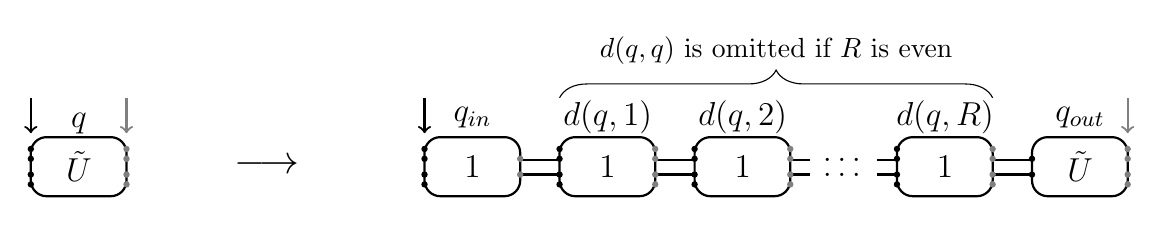
\begin{tikzpicture}[scale=0.5]
\begin{scope}[xshift=-10 cm]       
\draw[rounded corners=2mm,thick] (0,0) rectangle (2.43cm,1.5 cm);  
  \foreach \x /\color in {0/black,2.43/gray}
{     \foreach \y in {1.2,.95,.55,.3}
{       \draw[fill=\color,draw=\color] (\x cm, \y cm) circle (.66mm);
    }} 
\node at (1.22cm, .75cm) {\large{$\tilde U$}};   
 \node at (1.22cm, 1.85cm){\large{$q$}};

\node at (6cm, 0.75cm) {\Large{$\longrightarrow$}};
\draw [->, thick, color=black] (0,2.5) --(0,1.6);
\draw [->, thick, color=gray] (2.43,2.5) --(2.43,1.6);
\end{scope}
\draw [decorate,decoration={brace,amplitude=10pt}] (3.43,2.5) -- (14.43,2.5) node [black,midway,yshift=17]  {$d(q,q)$ is omitted if $R$ is even};
\draw [->, thick, color=black] (0,2.5) --(0,1.6);
\draw [->, thick, color=gray] (17.86,2.5) --(17.86,1.6);
  % The connections 
 \foreach \y in {0.925,.55}{  
  \draw[thick] (2.43,\y) -- (3.43,\y);
	\draw[thick] (5.86,\y) -- (6.86,\y);	
	\draw[thick] (14.43,\y) -- (15.43,\y);
	\draw[thick] (9.29,\y) -- (9.79,\y);
	\draw[thick] (11.5,\y) -- (12,\y);
	\node at (10.6,\y){\large{$\ldots$}};
}
%\draw[thick,looseness = 200] (0,1.2) to [out = 180, in = 100] (-.01,1.2);
  % The two rectangles 

%  15.43/\tilde U/q_{\mathrm{out}}
\draw[rounded corners=2mm,thick] (0,0) rectangle (2.43cm,1.5 cm);  
{     \foreach \y in {1.2,.95,.55,.3}
{       \draw[fill=black,draw=black] (0 cm, \y cm) circle (.66mm);
  }} 
  {     \foreach \y in {.95,.55}
{       \draw[fill=gray,draw=gray] (2.43 cm, \y cm) circle (.66mm);
  }} 
  \node at (1.22cm, .75cm) {\large{$1$}};   
 \node at (1.22cm, 2cm){\large{$q_{\text{in}}$}};   
 
 
 \begin{scope}[xshift=15.43 cm]
 \draw[rounded corners=2mm,thick] (0,0) rectangle (2.43cm,1.5 cm);  
{     \foreach \y in  {.95,.55}
{       \draw[fill=black,draw=black] (0 cm, \y cm) circle (.66mm);
  }} 
  {     \foreach \y in{1.2,.95,.55,.3}
{       \draw[fill=gray,draw=gray] (2.43 cm, \y cm) circle (.66mm);
  }} 
  \node at (1.22cm, .75cm) {\large{$\tilde{U}$}};   
 \node at (1.22cm, 2cm){\large{$q_{\text{out}}$}};   
 \end{scope}
 
 % the inner d(q,s) 
 \foreach \offset/\unitary/\label in {3.43/1/{d(q,1)},6.86/1/{d(q,2)},12/1/{d(q,R)}}
{   
\begin{scope}[xshift=\offset cm]       
\draw[rounded corners=2mm,thick] (0,0) rectangle (2.43cm,1.5 cm);  
  \foreach \x /\color in {0/black,2.43/gray}
{     \foreach \y in {1.2,.95,.55,.3}
{       \draw[fill=\color,draw=\color] (\x cm, \y cm) circle (.66mm);
    }} 
  \node at (1.22cm, .75cm) {\large{$\unitary$}};   
 \node at (1.22cm, 2cm){\large{$\label$}};   
\end{scope}}   
\end{tikzpicture}
\caption[Step 1 in $G^\square$ construction]{The first step in constructing the gate diagram of $G^{\square}$
from that of $G$ is to replace each diagram element as shown. The
four input nodes (black arrow) and four output nodes (grey arrow)
on the left-hand side are identified with nodes on the right-hand
side as shown.\label{fig:replace_gate_diagram}}
\end{figure}

\begin{figure}
\centering
\subfloat[b][$\{q,s\}\in E(G^{\text{occ}}),\,q<s$]{
  \label{fig:add_edgesA}
  \tikzsetnextfilename{MP_add_edgesA}
  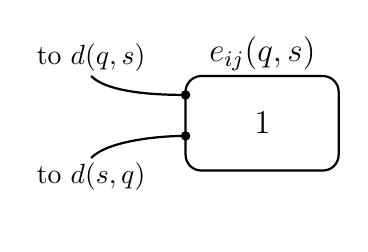
\begin{tikzpicture}[baseline=(X.base),scale=0.8]
\node at (0,0) (X){};
\begin{scope}[xshift=0cm]       
\draw[rounded corners=2mm,thick] (0,0) rectangle (2.43cm,1.5 cm);  
\foreach \y in {1.2,.55}
{       \draw[fill=black,draw=black] (0 cm, \y cm) circle (.66mm);
    }
\node at (1.22cm, .75cm) {\large{$1$}};   
 \node at (1.22cm, 1.85cm){\large{$e_{ij}(q,s)$}};
\draw[thick,looseness=.66] (0cm,1.2cm) to [out=180,in=-45] (-1.5cm,1.5cm);
\node at (-1.5,1.8){to $d(q,s)$};
\draw[thick,looseness=.66] (0cm,0.55cm) to [out=180,in=45] (-1.5cm,0.2cm);
\node at (-1.5,-0.1){to $d(s,q)$};
\end{scope}
\node at (0,-0.7){};
\end{tikzpicture}
}
\hspace{.5cm}
\subfloat[b][$\{q,s\}\notin E(G^{\text{occ}})$]{
  \label{fig:add_edgesB}  
  \tikzsetnextfilename{MP_add_edgesB}
  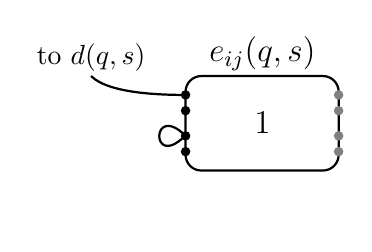
\begin{tikzpicture}[baseline=(X.base),scale=0.8]
\node at (0,0) (X){};

\begin{scope}[xshift=0cm]       
\draw[rounded corners=2mm,thick] (0,0) rectangle (2.43cm,1.5 cm);  
  \foreach \x /\color in {0/black,2.43/gray}
{     \foreach \y in {1.2,.95,.55,.3}
{       \draw[fill=\color,draw=\color] (\x cm, \y cm) circle (.66mm);
    }} 
\node at (1.22cm, .75cm) {\large{$1$}};   
 \node at (1.22cm, 1.85cm){\large{$e_{ij}(q,s)$}};
\draw[thick,looseness=.66] (0cm,1.2cm) to [out=180,in=-45] (-1.5cm,1.5cm);
\node at (-1.5,1.8){to $d(q,s)$};
\draw[thick,looseness = 200] (0,0.55) to [out = 135, in = 225] (-.01,0.55);
\end{scope}
\node at (0,-0.7){};
\end{tikzpicture}
}
\hspace{.5cm}
\subfloat[b][]{
  \label{fig:add_edgesC}
  \tikzsetnextfilename{MP_add_edgesC}
  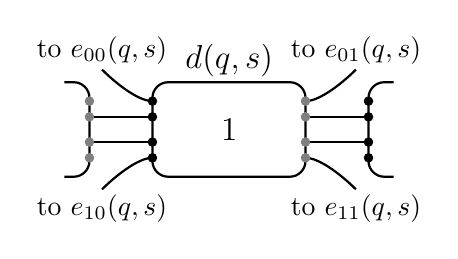
\begin{tikzpicture}[baseline=(X.base),scale=0.8]
\node at (0,0) (X){};
\draw[thick,looseness=.66] (0cm,1.2cm) to [out=180,in=-45] (-0.8cm,1.7cm);
\node at (-0.8cm,2cm){to $e_{00}(q,s)$};
\draw[thick,looseness=.66] (0cm,0.3cm) to [out=180,in=45] (-0.8cm,-0.2cm);
\node at (-0.8cm,-0.5cm){to $e_{10}(q,s)$};

\draw[thick,looseness=.66] (2.43cm,1.2cm) to [out=0,in=225] (3.23cm,1.7cm);
\node at (3.23cm,2cm){to $e_{01}(q,s)$};
\draw[thick,looseness=.66] (2.43cm,0.3cm) to [out=0,in=135] (3.23cm,-0.2cm);
\node at (3.23cm,-0.5cm){to $e_{11}(q,s)$};
\draw[thick] (-1,0.95)--(0,0.95);
\draw[thick] (-1,0.55)--(0,0.55);
\draw[thick] (2.43,0.95)--(3.43,0.95);
\draw[thick] (2.43,0.55)--(3.43,0.55);
\node at (0,-0.7){};
\begin{scope}
\clip (-1.4,-0.1) rectangle (3.83,2.1);
     
\draw[rounded corners=2mm,thick] (0,0) rectangle (2.43cm,1.5 cm);  
  \foreach \x /\color in {0/black,2.43/gray}
{     \foreach \y in {1.2,.95,.55,.3}
{       \draw[fill=\color,draw=\color] (\x cm, \y cm) circle (.66mm);
    }} 
\node at (1.22cm, .75cm) {\large{$1$}};   
 \node at (1.22cm, 1.85cm){\large{$d(q,s)$}};
\begin{scope}[xshift=3.43cm]
\draw[rounded corners=2mm,thick] (0,0) rectangle (2.43cm,1.5 cm);  
  \foreach \x /\color in {0/black,2.43/gray}
{     \foreach \y in {1.2,.95,.55,.3}
{       \draw[fill=\color,draw=\color] (\x cm, \y cm) circle (.66mm);
    }} 
\node at (1.22cm, .75cm) {\large{$1$}};   
 \node at (1.22cm, 1.85cm){\large{$d(q,\widehat{q})$}};
\end{scope}
\begin{scope}[xshift=-3.43cm]
\draw[rounded corners=2mm,thick] (0,0) rectangle (2.43cm,1.5 cm);  
  \foreach \x /\color in {0/black,2.43/gray}
{     \foreach \y in {1.2,.95,.55,.3}
{       \draw[fill=\color,draw=\color] (\x cm, \y cm) circle (.66mm);
    }} 
\node at (1.22cm, .75cm) {\large{$1$}};   
\node at (1.22cm, 1.85cm){\large{$d(q,s)$}};
\end{scope}
\end{scope}
\end{tikzpicture}
}
\caption[Step 4 in $G^\square$ construction]{Edges and self-loops added in step 4 of the construction of the gate diagram of $G^{\square}$. When $\{q,s\}\in E(G^{\text{occ}})$ with $q<s$, we add two outgoing edges to $e_{ij}(q,s)$ as shown in \subfig{add_edgesA}. Note that if $q>s$ and $\{q,s\}\in E(G^{\text{occ}})$ then $e_{ij}(q,s)=e_{ji}(s,q)$. When $\{q,s\}\notin E(G^{\text{occ}})$ we add a self-loop and a single outgoing edge from $e_{ij}(q,s)$ as shown in \subfig{add_edgesB}. Each diagram element $d(q,s)$ has eight outgoing edges (four of which are added in step 4), as shown in \subfig{add_edgesC}.\label{fig:add_edges}}
\end{figure}

The set of diagram elements in the gate graph for $G^{\square}$ is indexed by
\begin{equation}
L^{\square}=Q_{\text{in}}\cup D\cup E_{\text{edges}}\cup E_{\text{non-edges}}\cup Q_{\text{out}}\label{eq:L_square}
\end{equation}
where
\begin{align}
Q_{\text{in}} & =\left\{ q_{\mathrm{in}}:q\in[R]\right\} \label{eq:Q_in}\\
D & =\left\{ d(q,s):\, q,s\in[R]\text{ and }q\neq s\text{ if }R\text{ is even}\right\} \label{eq:defn_of D}\\
E_{\text{edges}} & =\left\{ e_{ij}(q,s):\,q,s\in[R],  i,j\in\{0,1\},\,\{q,s\}\in E(G^{\text{occ}})\text{ and }q<s\right\} \nonumber \\
E_{\text{non-edges}} & =\left\{ e_{ij}(q,s):\, q,s\in[R], i,j\in\{0,1\},\,\{q,s\}\notin E(G^{\text{occ}})\text{ and }q\neq s\text{ if }R\text{ is even}\right\} \nonumber \\
Q_{\text{out}} & =\left\{ q_{\mathrm{out}}:q\in[R]\right\} .\label{eq:Q_out}
\end{align}
The total number of diagram elements in $G^{\square}$ is 
\begin{align}
|L^{\square}| & =|Q_{\text{in}}|+|D|+|E_{\text{edges}}|+|E_{\text{non-edges}}|+|Q_{\text{out}}|\\
 & =\begin{cases}
R+R^{2}+4|E(G^{\text{occ}})|+4\left(R^{2}-2|E(G^{\text{occ}})|\right)+R & R\text{ odd}\\
R+R\left(R-1\right)+4|E(G^{\text{occ}})|+4\left(R(R-1)-2|E(G^{\text{occ}})|\right)+R & R\text{ even}
\end{cases}\\
 & =\begin{cases}
5R^{2}+2R-4|E(G^{\text{occ}})| & R\text{ odd}\\
5R^{2}-3R-4|E(G^{\text{occ}})| & R\text{ even}.
\end{cases}
\end{align}
In both cases this is upper bounded by $7R^2$ as claimed in the statement of the Lemma. Write 
\begin{equation}
A(G^{\square})=\sum_{l\in L^{\square}}|l\rangle\langle l|\otimes A(g_{l})+h_{\mathcal{S}^{\square}}+h_{\mathcal{E}^{\square}}\label{eq:A_G_squAre}
\end{equation}
where $g_l$ corresponds to the diagram element labeled $l\in L^{\square}$, $\mathcal{S}^{\square}$ and $\mathcal{E}^{\square}$ are the sets of self-loops and edges in the gate diagram for $G^{\square}$. 

We now focus on the input nodes of diagram elements in $Q_{\text{in}}$ and the output nodes of the diagram elements in $Q_{\text{out}}$. These are the nodes indicated by the black and grey arrows in \fig{replace_gate_diagram}. Write $\mathcal{E}^{0}\subset\mathcal{E}^{\square}$ and $\mathcal{S}^{0}\subset\mathcal{S^{\square}}$ for the sets of edges and self-loops that are incident on these nodes in the gate diagram for $G^{\square}$. Note that the sets $\mathcal{E}^{0}$ and $\mathcal{S}^{0}$ are in one-to-one correspondence with (respectively) the sets $\mathcal{E}^{G}$ and $\mathcal{S}^{G}$ of edges and self-loops in the gate diagram for $G$ (by definition). The other edges and self-loops in $G^{\square}$ do not depend on the sets of edges and self-loops in $G$, as they are created in our effort to enforce the occupancy constraints. Writing
\begin{equation}
\mathcal{S}^{\triangle}=\mathcal{S}^{\square}\setminus S^{0}\qquad\mathcal{E}^{\triangle}=\mathcal{E}^{\square}\setminus\mathcal{E}^{0},
\end{equation}
we have 
\begin{equation}
h_{\mathcal{S}^{\square}}=h_{\mathcal{S}^{0}}+h_{\mathcal{S}^{\triangle}}\qquad h_{\mathcal{E}^{\square}}=h_{\mathcal{E}^{0}}+h_{\mathcal{E}^{\triangle}}.\label{eq:h_se_square}
\end{equation}

It will be useful to define several graphs that only depend on the occupancy constraints as a stepping stone in order to understand $\lambda_N^1(G^\square)$.  In particular, we will first examine the gate graph that only has the self-loops added during the transformation from $G$ to $G^{\square}$, namely the self-loops on nodes in $\mathcal{S}^{\triangle}$, as this graph has a particularly simple ground space, and we will label this graph $G^{\diamondsuit}$.  We will then analyze the graph that arises by adding the edges of $\mathcal{E}^{\triangle}$ to $G^\diamondsuit$, and we will label this graph by $G^{\triangle}$.  With these foundational graphs understood (and in particular understanding their $N$-particle frustration-free ground states), we will then easily understand the ground states and ground energies of $G^{\square}$ in term of the ground energies of $G$.

Along these lines, we will define the gate diagram for $G^{\diamondsuit}$ to be the diagram with all of the elements labeled by $L^{\square}$, and only include the self-loops in $\mathcal{S}^{\triangle}$.  We then have that the adjacency matrix for $G^{\diamondsuit}$ is 
\begin{equation}
  A(G^{\diamondsuit}) = \sum_{\ell \in L^{\square}} \ketbra{\ell}{\ell} \otimes A(g_\ell) + h_{\mathcal{S}^\triangle}\label{eq:A_G_diamond_defn}.
\end{equation}

We can also define the gate diagram for $G^{\triangle}$ to be the same as for $G^{\diamondsuit}$, but including the edges in $\mathcal{E}^{\triangle}$.  We can then define the adjacency matrix for $G^{\triangle}$ as
\begin{equation}
  A(G^{\triangle})=\sum_{l\in L^{\square}}|l\rangle\langle l|\otimes A(g_{l})+h_{\mathcal{S}^{\triangle}}+h_{\mathcal{E}^{\triangle}}.\label{eq:A_g_triangle}
\end{equation}
Note that $G^{\triangle}=G^{\square}$ whenever the gate diagram for $G$ contains no edges or self-loops. 


We provide an example of this construction in \fig{example_G_Gtilde} (which shows a gate graph and an occupancy constraints graph) and \fig{big_example_G_square} (which describes the derived gate graphs $G^{\square}$, $G^{\triangle}$, and $G^{\diamondsuit}$).

\todo{completely fix these example graphs}

\begin{figure}
\centering
\subfloat[][]{
  \label{fig:example_G_GtildeA}
  \tikzsetnextfilename{MP_example_G_GtildeA}
  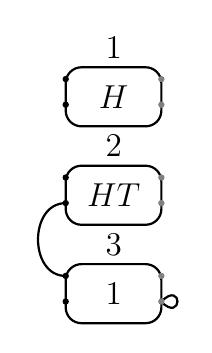
\begin{tikzpicture}[scale=0.5]
% The gate graph G 
\draw[thick,looseness=1.3] (0,-1.95cm) to [out=180,in=180] (0,-3.8cm);
\draw[thick,looseness = 200] (2.43,-4.45) to [out = 45, in = -45] (2.42,-4.45);  
 \foreach \offset/\unitary/\label in {0/H/1,-2.5/HT/2,-5/1/3}
{   
\begin{scope}[yshift=\offset cm]       
\draw[rounded corners=2mm,thick] (0,0) rectangle (2.43cm,1.5 cm);  
  \foreach \x /\color in {0/black,2.43/gray}
{     \foreach \y in {1.2,.55}
{       \draw[fill=\color,draw=\color] (\x cm, \y cm) circle (.66mm);
    }} 
  \node at (1.22cm, .75cm) {\large{$\unitary$}};   
 \node at (1.22cm, 2cm){\large{$\label$}};   
\end{scope}}  
\end{tikzpicture}
}
\hspace{4cm}
\subfloat[][]{
  \label{fig:example_G_GtildeB}
  \tikzsetnextfilename{MP_example_G_GtildeB}
  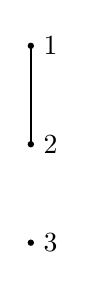
\begin{tikzpicture}[scale=0.5]
% The graph G_tilde
 \draw[fill=black,draw=black] (1,0) circle (.66mm);
\node at (1.5,0) {1};
 \draw[fill=black,draw=black] (1,-2.5) circle (.66mm);
\node at (1.5,-2.5) {2};
 \draw[fill=black,draw=black] (1,-5) circle (.66mm);
\node at (1.5,-5) {3};
\draw[thick] (1,0) -- (1,-2.5);
\end{tikzpicture}
}
\caption[Example occupancy constraints]{An example \subfig{example_G_GtildeA} Gate diagram for a gate graph $G$ and \subfig{example_G_GtildeB} Occupancy constraints graph $G^{\text{occ}}$. In the text we describe how these two ingredients are mapped to a gate graph $G^{\square}$; the gate diagram for $G^{\square}$ is shown in \fig{big_example_G_square}.\label{fig:example_G_Gtilde}}
\end{figure}

\begin{figure}
  \tikzsetnextfilename{MP_big_example_G_square}
  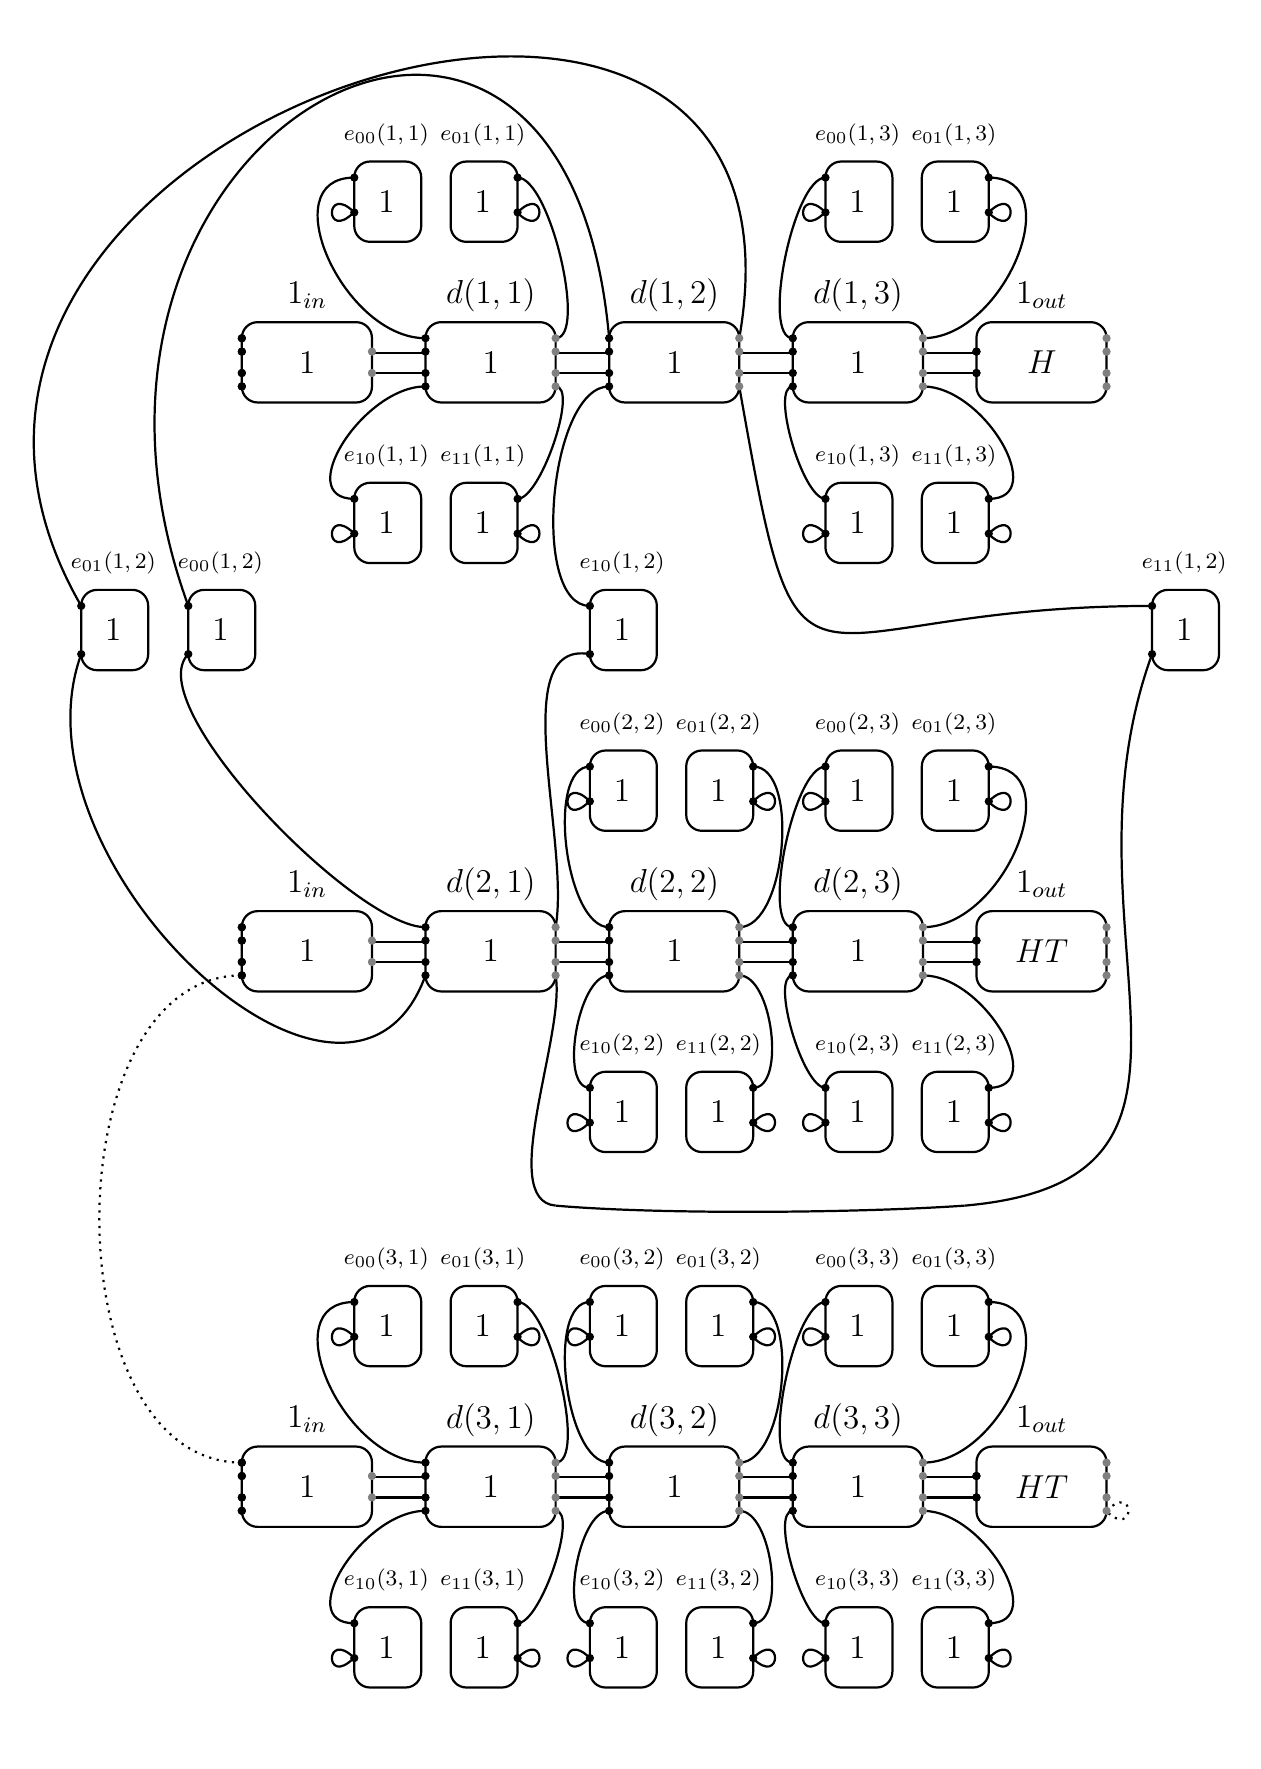
\begin{tikzpicture}[scale=0.68]
\path[use as bounding box](-4,-25) rectangle (18.5,7);
%%%%%%%%%%%%%%%%%%%%%%%%%%%%%%%%% q=1/2 shared elements
\begin{scope}[yshift=-5cm]
%%%%%%%% e00
\foreach \offset/\unitary/\label in
{-1/1/{e_{00}(1,2)}}
{   
\begin{scope}[xshift=\offset cm]       
\draw[rounded corners=2mm,thick] (0,0) rectangle (1.25cm,1.5 cm);  
   \foreach \y in {1.2,.3}
{       \draw[fill=black,draw=black] (0 cm, \y cm) circle (.66mm);
    } 
  \node at (0.6cm, .75cm) {\large{$\unitary$}};   
 \node at (0.6cm, 2cm){\footnotesize{$\label$}};
\end{scope}}
%%%%%%%%%%%%% e10
\foreach \offset/\unitary/\label in
{-3/1/{e_{01}(1,2)}}
{   
\begin{scope}[xshift=\offset cm]       
\draw[rounded corners=2mm,thick] (0,0) rectangle (1.25cm,1.5 cm);  
   \foreach \y in {1.2,.3}
{       \draw[fill=black,draw=black] (0 cm, \y cm) circle (.66mm);
    } 
  \node at (0.6cm, .75cm) {\large{$\unitary$}};   
 \node at (0.6cm, 2cm){\footnotesize{$\label$}};
\end{scope}}
\begin{scope}
%%%%%%%% e01
\foreach \offset/\unitary/\label in
{6.5/1/{e_{10}(1,2)}}
{   
\begin{scope}[xshift=\offset cm]       
\draw[rounded corners=2mm,thick] (0,0) rectangle (1.25cm,1.5 cm);  
   \foreach \y in {1.2,.3}
{       \draw[fill=black,draw=black] (0 cm, \y cm) circle (.66mm);
    } 
  \node at (0.6cm, .75cm) {\large{$\unitary$}};   
 \node at (0.6cm, 2cm){\footnotesize{$\label$}};
\end{scope}}
%%%%%%%%%%%%% e11
\foreach \offset/\unitary/\label in
{17/1/{e_{11}(1,2)}}
{   
\begin{scope}[xshift=\offset cm]       
\draw[rounded corners=2mm,thick] (0,0) rectangle (1.25cm,1.5 cm);  
   \foreach \y in {1.2,.3}
{       \draw[fill=black,draw=black] (0 cm, \y cm) circle (.66mm);
    } 
  \node at (0.6cm, .75cm) {\large{$\unitary$}};   
 \node at (0.6cm, 2cm){\footnotesize{$\label$}};
\end{scope}}
\end{scope}

%%%%%%
% these are the stuff
\draw[thick,looseness = 2.6] (6.86,6.2) to [out = 95, in = 110] (-1,1.2); 
\draw[thick,looseness = 0.5] (3.43,-4.8) to [out = 180, in = 225] (-1,0.3); 
\draw[thick,looseness = 1.2] (3.43,-5.7) to [out = 250, in = 250] (-3,0.3); 
\draw[thick,looseness = 0.7] (6.86,5.3) to [out = 180, in = 180] (6.5,1.2); 
\draw[thick,looseness = 0.8] (5.86,-4.8) to [out = 80, in = 170] (6.5,0.3); 

\draw[thick,looseness = 2] (9.29,5.3) to [out =-80, in = 180] (17,1.2);  
\draw[thick,looseness = 1.3] (13.5,-10) to [out =5, in = 250] (17,0.3);
\draw[thick,looseness = 0.66] (5.86,-10) to [out =-5, in = 184] (13.5,-10);
\draw[thick,looseness = 0.66] (5.86,-5.7) to [out =-80, in = 175] (5.86,-10);
\draw[thick,looseness = 2] (9.29,6.2) to [out =80, in = 120] (-3,1.2); 
\end{scope}

%%%%%%%%%%%%%%%%%%%%%%%%%%%%%%%%% q=1
\begin{scope}
\begin{scope}[yshift=3cm]
% The rectangles above q=1, odd ones
\foreach \offset/\unitary/\label in
{2.1/1/{e_{00}(1,1)},10.9/1/{e_{00}(1,3)}}
{   
\begin{scope}[xshift=\offset cm]       
\draw[rounded corners=2mm,thick] (0,0) rectangle (1.25cm,1.5 cm);  
  \foreach \y in {1.2,.55}
{       \draw[fill=black,draw=black] (0 cm, \y cm) circle (.66mm);
  } 
  \node at (0.6cm, .75cm) {\large{$\unitary$}};   
 \node at (0.6cm, 2cm){\footnotesize{$\label$}};
\draw[thick,looseness = 200] (0,0.55) to [out = 135, in = 225] (-.01,0.55);  
\end{scope}}  
% The rectangles above q=1, even ones
\foreach \offset/\unitary/\label in
{3.9/1/{e_{01}(1,1)},12.7/1/{e_{01}(1,3)}}
{   
\begin{scope}[xshift=\offset cm]       
\draw[rounded corners=2mm,thick] (0,0) rectangle (1.25cm,1.5 cm);  
  \foreach \y in {1.2,.55}
  {       \draw[fill=black,draw=black] (1.25 cm, \y cm) circle (.66mm);
    }
  \node at (0.6cm, .75cm) {\large{$\unitary$}};   
 \node at (0.6cm, 2cm){\footnotesize{$\label$}};
\draw[thick,looseness = 200] (1.25,0.55) to [out = 45, in = -45] (1.24,0.55);  
\end{scope}} 

 
\draw[thick,looseness = 1.2] (3.43,-1.8) to [out = 180, in = 180] (2.1,1.2); 
\draw[thick,looseness = 0.5] (5.86,-1.8) to [out = 0, in = 0] (5.15,1.2); 
\draw[thick,looseness = 0.5] (10.29,-1.8) to [out = 180, in = 180] (10.9,1.2); 
\draw[thick,looseness = 1.2] (12.72,-1.8) to [out = 0, in = 0] (13.95,1.2); 
\end{scope}
\begin{scope}[yshift=-3cm]
% The rectangles below q=1, odd ones
\foreach \offset/\unitary/\label in
{2.1/1/{e_{10}(1,1)},10.9/1/{e_{10}(1,3)}}
{   
\begin{scope}[xshift=\offset cm]       
\draw[rounded corners=2mm,thick] (0,0) rectangle (1.25cm,1.5 cm);  
  \foreach \y in {1.2,.55}
{       \draw[fill=black,draw=black] (0 cm, \y cm) circle (.66mm);
  } 
  \node at (0.6cm, .75cm) {\large{$\unitary$}};   
 \node at (0.6cm, 2cm){\footnotesize{$\label$}};
\draw[thick,looseness = 200] (0,0.55) to [out = 135, in = 225] (-.01,0.55);  
\end{scope}}  

% The rectangles below q=1, even ones
\foreach \offset/\unitary/\label in
{3.9/1/{e_{11}(1,1)},12.7/1/{e_{11}(1,3)}}
{   
\begin{scope}[xshift=\offset cm]       
\draw[rounded corners=2mm,thick] (0,0) rectangle (1.25cm,1.5 cm);  
  \foreach \y in {1.2,.55}
  {       \draw[fill=black,draw=black] (1.25 cm, \y cm) circle (.66mm);
    }
  \node at (0.6cm, .75cm) {\large{$\unitary$}};   
 \node at (0.6cm, 2cm){\footnotesize{$\label$}};
\draw[thick,looseness = 200] (1.25,0.55) to [out = 45, in = -45] (1.24,0.55);  
\end{scope}} 


\draw[thick,looseness = 1.2] (3.43,3.3) to [out = 180, in = 180] (2.1,1.2); 
\draw[thick,looseness = 0.5] (5.86,3.3) to [out = 0, in = 0] (5.15,1.2); 
\draw[thick,looseness = 0.5] (10.29,3.3) to [out = 180, in = 180] (10.9,1.2); 
\draw[thick,looseness = 1.2] (12.72,3.3) to [out = 0, in = 0] (13.95,1.2); 
\end{scope}
  % The connections 
 \foreach \y in {0.925,.55}{  
  \draw[thick] (2.43,\y) -- (3.43,\y);
	\draw[thick] (5.86,\y) -- (6.86,\y);	
	\draw[thick] (9.29,\y) -- (10.29,\y);
	\draw[thick] (12.72,\y) -- (13.72,\y);
}
  % The rectangles 
  

\draw[rounded corners=2mm,thick] (0,0) rectangle (2.43cm,1.5 cm);  
  \foreach \x /\color in {0/black,2.43/gray}
  \foreach \y in {1.2,.95,.55,.3}
  {       \draw[fill=black,draw=black] (0 cm, \y cm) circle (.66mm);
  }
  \foreach \y in {.95,.55}
  {       \draw[fill=gray,draw=gray] (2.43 cm, \y cm) circle (.66mm);
  } 
  \node at (1.22cm, .75cm) {\large{$1$}};   
 \node at (1.22cm, 2cm){\large{$1_{\text{in}}$}}; 
 
\begin{scope}[xshift = 13.72 cm] 
 \draw[rounded corners=2mm,thick] (0,0) rectangle (2.43cm,1.5 cm);  
  \foreach \x /\color in {0/black,2.43/gray}
  \foreach \y in {.95,.55}
  {       \draw[fill=black,draw=black] (0 cm, \y cm) circle (.66mm);
  }
  \foreach \y in {1.2,.95,.55,.3}
  {       \draw[fill=gray,draw=gray] (2.43 cm, \y cm) circle (.66mm);
  } 
  \node at (1.22cm, .75cm) {\large{$H$}};   
 \node at (1.22cm, 2cm){\large{$1_{\text{out}}$}};   
\end{scope}

  
 \foreach \offset/\unitary/\label in {3.43/1/{d(1,1)},6.86/1/{d(1,2)},10.29/1/{d(1,3)}}
{   
\begin{scope}[xshift=\offset cm]       
\draw[rounded corners=2mm,thick] (0,0) rectangle (2.43cm,1.5 cm);  
  \foreach \x /\color in {0/black,2.43/gray}
{     \foreach \y in {1.2,.95,.55,.3}
{       \draw[fill=\color,draw=\color] (\x cm, \y cm) circle (.66mm);
    }} 
  \node at (1.22cm, .75cm) {\large{$\unitary$}};   
 \node at (1.22cm, 2cm){\large{$\label$}};   
\end{scope}}  
\end{scope}

%%%%%%%%%%%%%%%%%%%%%%%%%%%%%%%%% q=2
\begin{scope}[yshift=-11cm]
\begin{scope}[yshift=3cm]



% The rectangles above q=2, odd ones
\foreach \offset/\unitary/\label in
{6.5/1/{e_{00}(2,2)},10.9/1/{e_{00}(2,3)}}
{   
\begin{scope}[xshift=\offset cm]       
\draw[rounded corners=2mm,thick] (0,0) rectangle (1.25cm,1.5 cm);  
  \foreach \y in {1.2,.55}
{       \draw[fill=black,draw=black] (0 cm, \y cm) circle (.66mm);
  } 
  \node at (0.6cm, .75cm) {\large{$\unitary$}};   
 \node at (0.6cm, 2cm){\footnotesize{$\label$}};
\draw[thick,looseness = 200] (0,0.55) to [out = 135, in = 225] (-.01,0.55);  
\end{scope}}   
\end{scope}
\begin{scope}[yshift=3cm]
% The rectangles above q=2, even ones
\draw[thick,looseness = 0.7] (6.86,-1.8) to [out = 180, in = 180] (6.5,1.2); 
\draw[thick,looseness = 0.75] (9.29,-1.8) to [out = 0, in = 0] (9.55,1.2); 
\draw[thick,looseness = 0.5] (10.29,-1.8) to [out = 180, in = 180] (10.9,1.2); 
\draw[thick,looseness = 1.2] (12.72,-1.8) to [out = 0, in = 0] (13.95,1.2); 
\foreach \offset/\unitary/\label in
{8.3/1/{e_{01}(2,2)},12.7/1/{e_{01}(2,3)}}
{   
\begin{scope}[xshift=\offset cm]       
\draw[rounded corners=2mm,thick] (0,0) rectangle (1.25cm,1.5 cm);  
  \foreach \y in {1.2,.55}
  {       \draw[fill=black,draw=black] (1.25 cm, \y cm) circle (.66mm);
    }
  \node at (0.6cm, .75cm) {\large{$\unitary$}};   
 \node at (0.6cm, 2cm){\footnotesize{$\label$}};
\draw[thick,looseness = 200] (1.25,0.55) to [out = 45, in = -45] (1.24,0.55);  
\end{scope}}   
\end{scope}
\begin{scope}[yshift=-3cm]
% The rectangles below q=2, odd ones
\foreach \offset/\unitary/\label in
{6.5/1/{e_{10}(2,2)},10.9/1/{e_{10}(2,3)}}
{   
\begin{scope}[xshift=\offset cm]       
\draw[rounded corners=2mm,thick] (0,0) rectangle (1.25cm,1.5 cm);  
  \foreach \y in {1.2,.55}
{       \draw[fill=black,draw=black] (0 cm, \y cm) circle (.66mm);
  } 
  \node at (0.6cm, .75cm) {\large{$\unitary$}};   
 \node at (0.6cm, 2cm){\footnotesize{$\label$}};
\draw[thick,looseness = 200] (0,0.55) to [out = 135, in = 225] (-.01,0.55);  
\end{scope}}  
\end{scope}
\begin{scope}[yshift=-3cm]
% The rectangles below q=2, even ones
\foreach \offset/\unitary/\label in
{8.3/1/{e_{11}(2,2)},12.7/1/{e_{11}(2,3)}}
{   
\begin{scope}[xshift=\offset cm]       
\draw[rounded corners=2mm,thick] (0,0) rectangle (1.25cm,1.5 cm);  
  \foreach \y in {1.2,.55}
  {       \draw[fill=black,draw=black] (1.25 cm, \y cm) circle (.66mm);
    }
  \node at (0.6cm, .75cm) {\large{$\unitary$}};   
 \node at (0.6cm, 2cm){\footnotesize{$\label$}};
\draw[thick,looseness = 200] (1.25,0.55) to [out = 45, in = -45] (1.24,0.55);  
\end{scope}}   
\draw[thick,looseness = 0.7] (6.86,3.3) to [out = 180, in = 180] (6.5,1.2); 
\draw[thick,looseness = 0.75] (9.29,3.3) to [out = 0, in = 0] (9.55,1.2); 
\draw[thick,looseness = 0.5] (10.29,3.3) to [out = 180, in = 180] (10.9,1.2); 
\draw[thick,looseness = 1.2] (12.72,3.3) to [out = 0, in = 0] (13.95,1.2); 
\end{scope}
  % The connections 
 \foreach \y in {0.925,.55}{  
  \draw[thick] (2.43,\y) -- (3.43,\y);
	\draw[thick] (5.86,\y) -- (6.86,\y);	
	\draw[thick] (9.29,\y) -- (10.29,\y);
	\draw[thick] (12.72,\y) -- (13.72,\y);
}
  % The rectangles 
  \draw[rounded corners=2mm,thick] (0,0) rectangle (2.43cm,1.5 cm);  
  \foreach \x /\color in {0/black,2.43/gray}
  \foreach \y in {1.2,.95,.55,.3}
  {       \draw[fill=black,draw=black] (0 cm, \y cm) circle (.66mm);
  }
  \foreach \y in {.95,.55}
  {       \draw[fill=gray,draw=gray] (2.43 cm, \y cm) circle (.66mm);
  } 
  \node at (1.22cm, .75cm) {\large{$1$}};   
 \node at (1.22cm, 2cm){\large{$1_{\text{in}}$}}; 
 
\begin{scope}[xshift = 13.72 cm] 
 \draw[rounded corners=2mm,thick] (0,0) rectangle (2.43cm,1.5 cm);  
  \foreach \x /\color in {0/black,2.43/gray}
  \foreach \y in {.95,.55}
  {       \draw[fill=black,draw=black] (0 cm, \y cm) circle (.66mm);
  }
  \foreach \y in {1.2,.95,.55,.3}
  {       \draw[fill=gray,draw=gray] (2.43 cm, \y cm) circle (.66mm);
  } 
  \node at (1.22cm, .75cm) {\large{$HT$}};   
 \node at (1.22cm, 2cm){\large{$1_{\text{out}}$}};   
\end{scope}
  
 \foreach \offset/\unitary/\label in {3.43/1/{d(2,1)},6.86/1/{d(2,2)},10.29/1/{d(2,3)}}
{   
\begin{scope}[xshift=\offset cm]       
\draw[rounded corners=2mm,thick] (0,0) rectangle (2.43cm,1.5 cm);  
  \foreach \x /\color in {0/black,2.43/gray}
{     \foreach \y in {1.2,.95,.55,.3}
{       \draw[fill=\color,draw=\color] (\x cm, \y cm) circle (.66mm);
    }} 
  \node at (1.22cm, .75cm) {\large{$\unitary$}};   
 \node at (1.22cm, 2cm){\large{$\label$}};   
\end{scope}}
\end{scope}

%%%%%%%%%%%%%%%%%%%%%%%%%%%%%%%%% q=3
\begin{scope}[yshift=-21cm]
%%%%%%%%%%%%% Edge and self-loop from G
\draw[thick,dotted,looseness = 200] (16.15,0.3) to [out = 45, in = -45] (16.14,0.3); 
\draw[thick,dotted,looseness = 1] (0,1.2) to [out =180, in = 180] (0,10.3);

\begin{scope}[yshift=3cm]
% The rectangles above q=3, odd ones
\foreach \offset/\unitary/\label in
{2.1/1/{e_{00}(3,1)},6.5/1/{e_{00}(3,2)},10.9/1/{e_{00}(3,3)}}
{   
\begin{scope}[xshift=\offset cm]       
\draw[rounded corners=2mm,thick] (0,0) rectangle (1.25cm,1.5 cm);  
  \foreach \y in {1.2,.55}
{       \draw[fill=black,draw=black] (0 cm, \y cm) circle (.66mm);
  } 
  \node at (0.6cm, .75cm) {\large{$\unitary$}};   
 \node at (0.6cm, 2cm){\footnotesize{$\label$}};
\draw[thick,looseness = 200] (0,0.55) to [out = 135, in = 225] (-.01,0.55);  
\end{scope}} 
\end{scope}
\begin{scope}[yshift=3cm]
% The rectangles above q=3, even ones
\foreach \offset/\unitary/\label in
{3.9/1/{e_{01}(3,1)},8.3/1/{e_{01}(3,2)},12.7/1/{e_{01}(3,3)}}
{   
\begin{scope}[xshift=\offset cm]       
\draw[rounded corners=2mm,thick] (0,0) rectangle (1.25cm,1.5 cm);  
  \foreach \y in {1.2,.55}
  {       \draw[fill=black,draw=black] (1.25 cm, \y cm) circle (.66mm);
    }
  \node at (0.6cm, .75cm) {\large{$\unitary$}};   
 \node at (0.6cm, 2cm){\footnotesize{$\label$}};
\draw[thick,looseness = 200] (1.25,0.55) to [out = 45, in = -45] (1.24,0.55);  
\end{scope}}  
\draw[thick,looseness = 1.2] (3.43,-1.8) to [out = 180, in = 180] (2.1,1.2); 
\draw[thick,looseness = 0.5] (5.86,-1.8) to [out = 0, in = 0] (5.15,1.2); 
\draw[thick,looseness = 0.7] (6.86,-1.8) to [out = 180, in = 180] (6.5,1.2); 
\draw[thick,looseness = 0.75] (9.29,-1.8) to [out = 0, in = 0] (9.55,1.2); 
\draw[thick,looseness = 0.5] (10.29,-1.8) to [out = 180, in = 180] (10.9,1.2); 
\draw[thick,looseness = 1.2] (12.72,-1.8) to [out = 0, in = 0] (13.95,1.2); 
\end{scope}
\begin{scope}[yshift=-3cm]
% The rectangles below q=3, odd ones
\foreach \offset/\unitary/\label in
{2.1/1/{e_{10}(3,1)},6.5/1/{e_{10}(3,2)},10.9/1/{e_{10}(3,3)}}
{   
\begin{scope}[xshift=\offset cm]       
\draw[rounded corners=2mm,thick] (0,0) rectangle (1.25cm,1.5 cm);  
  \foreach \y in {1.2,.55}
{       \draw[fill=black,draw=black] (0 cm, \y cm) circle (.66mm);
  } 
  \node at (0.6cm, .75cm) {\large{$\unitary$}};   
 \node at (0.6cm, 2cm){\footnotesize{$\label$}};
\draw[thick,looseness = 200] (0,0.55) to [out = 135, in = 225] (-.01,0.55);  
\end{scope}}   
\end{scope}
\begin{scope}[yshift=-3cm]
% The rectangles below q=3, even ones
\foreach \offset/\unitary/\label in
{3.9/1/{e_{11}(3,1)},8.3/1/{e_{11}(3,2)},12.7/1/{e_{11}(3,3)}}
{   
\begin{scope}[xshift=\offset cm]       
\draw[rounded corners=2mm,thick] (0,0) rectangle (1.25cm,1.5 cm);  
  \foreach \y in {1.2,.55}
  {       \draw[fill=black,draw=black] (1.25 cm, \y cm) circle (.66mm);
    }
  \node at (0.6cm, .75cm) {\large{$\unitary$}};   
 \node at (0.6cm, 2cm){\footnotesize{$\label$}};
\draw[thick,looseness = 200] (1.25,0.55) to [out = 45, in = -45] (1.24,0.55);  
\end{scope}}     
\draw[thick,looseness = 1.2] (3.43,3.3) to [out = 180, in = 180] (2.1,1.2); 
\draw[thick,looseness = 0.5] (5.86,3.3) to [out = 0, in = 0] (5.15,1.2); 
\draw[thick,looseness = 0.7] (6.86,3.3) to [out = 180, in = 180] (6.5,1.2); 
\draw[thick,looseness = 0.75] (9.29,3.3) to [out = 0, in = 0] (9.55,1.2); 
\draw[thick,looseness = 0.5] (10.29,3.3) to [out = 180, in = 180] (10.9,1.2); 
\draw[thick,looseness = 1.2] (12.72,3.3) to [out = 0, in = 0] (13.95,1.2); 
\end{scope}
  % The connections 
 \foreach \y in {0.925,.55}{  
  \draw[thick] (2.43,\y) -- (3.43,\y);
	\draw[thick] (5.86,\y) -- (6.86,\y);	
	\draw[thick] (9.29,\y) -- (10.29,\y);
	\draw[thick] (12.72,\y) -- (13.72,\y);
}
  % The rectangles 
    \draw[rounded corners=2mm,thick] (0,0) rectangle (2.43cm,1.5 cm);  
  \foreach \x /\color in {0/black,2.43/gray}
  \foreach \y in {1.2,.95,.55,.3}
  {       \draw[fill=black,draw=black] (0 cm, \y cm) circle (.66mm);
  }
  \foreach \y in {.95,.55}
  {       \draw[fill=gray,draw=gray] (2.43 cm, \y cm) circle (.66mm);
  } 
  \node at (1.22cm, .75cm) {\large{$1$}};   
 \node at (1.22cm, 2cm){\large{$1_{\text{in}}$}}; 
 
\begin{scope}[xshift = 13.72 cm] 
 \draw[rounded corners=2mm,thick] (0,0) rectangle (2.43cm,1.5 cm);  
  \foreach \x /\color in {0/black,2.43/gray}
  \foreach \y in {.95,.55}
  {       \draw[fill=black,draw=black] (0 cm, \y cm) circle (.66mm);
  }
  \foreach \y in {1.2,.95,.55,.3}
  {       \draw[fill=gray,draw=gray] (2.43 cm, \y cm) circle (.66mm);
  } 
  \node at (1.22cm, .75cm) {\large{$HT$}};   
 \node at (1.22cm, 2cm){\large{$1_{\text{out}}$}};   
\end{scope}
  
 \foreach \offset/\unitary/\label in {3.43/1/{d(3,1)},6.86/1/{d(3,2)},10.29/1/{d(3,3)}}
{   
\begin{scope}[xshift=\offset cm]       
\draw[rounded corners=2mm,thick] (0,0) rectangle (2.43cm,1.5 cm);  
  \foreach \x /\color in {0/black,2.43/gray}
{     \foreach \y in {1.2,.95,.55,.3}
{       \draw[fill=\color,draw=\color] (\x cm, \y cm) circle (.66mm);
    }} 
  \node at (1.22cm, .75cm) {\large{$\unitary$}};   
 \node at (1.22cm, 2cm){\large{$\label$}};   
\end{scope}}  
\end{scope}
\end{tikzpicture}
\caption[$G^\square$ example]{The gate diagram for $G^{\triangle}$ (only solid lines) and $G^{\square}$ (including dotted lines) derived from the example gate graph $G$ and occupancy constraints graph $G^{\text{occ}}$ from \fig{example_G_Gtilde}. The gate diagram for $G^{\diamondsuit}$ is obtained from that of $G^{\triangle}$ by removing all edges (but leaving the undotted self-loops).\label{fig:big_example_G_square}}
\end{figure}


%=============================================================================
\subsection{The gate graph $G^{\diamondsuit}$}
\label{sec:The-gate-graph_G_DIAMOND}

With the various graphs well defined, let us now find the ground states of $A(G^{\diamondsuit})$.  We know from $\eq{A_G_diamond_defn}$ that each component of $G^{\diamondsuit}$ is a diagram element $g_l$, with self-loops on some of the nodes.  Using \lem{diagram_element_ground}, we can then see that each component of $G^{\diamondsuit}$ has at most 4 orthonormal $e_1$-energy eigenstates, and that the minimum energy is $e_1$.

More concretely, for each diagram element labeled by $l\in L^{\square}$ in $A(G^{\diamondsuit})$, we can write $g_{l}'$ for the graph with adjacency matrix
\begin{equation}
  A(g_{l}')=A(g_{l})+|1,2k \rangle\langle 1,2k+2|\otimes\II_{16}
\end{equation}
(i.e., $g_l$ with $16$ self-loops added), and note that each component of $G^{\diamondsuit}$ is either $g_{l}$ or $g_{l}'$.  

We can then use \lem{diagram_element_ground} to see that $A(g_{\ell})$ has four orthonormal $e_{1}$-energy ground states for each $\ell$ namely $\ket{\overline{\psi_{z,a}}}$ for $z,a\in\FF_2$, as defined in \eq{psi0m}, \eq{psi1m}, using the transform of \eq{phi_copy_transform}.  As the states with $z= 0$ are in the nullspace of $\ketbra{1,2k}{1,2k}\otimes \II_{16}$, while the operator is strictly positive for the states with $z=1$, we can see that the ground space of $A(g_l')$ is spanned by the states $\ket{\overline{\psi_{0,a}}}$ for $a\in\FF_2$.  If we now label the states by the $l\in L^{\square}$,  (i.e., $|\psi_{z,a}^{l}\rangle=|l\rangle|\overline{\psi_{z,a}}\rangle$, we can choose a basis $\mathcal{W}$ for the $e_{1}$-energy ground space of $A(G^{\diamondsuit})$ where each basis vector is supported on one of the components:
\begin{equation}
  \mathcal{W}= \big\{ |\psi_{0,a}^{l}\rangle:\, a\in\FF_2,\, l\in E_{\text{non-edges}}\big\} \bigcup \big\{ |\psi_{z,a}^{l}\rangle:\, z,a\in\FF_2,\, l\in L^{\square}\setminus E_{\text{non-edges}}\big\} .\label{eq:definition_of_W}
\end{equation}
The eigenvalue gap of $A(G^{\diamondsuit})$ is equal to that of either $A(g_{l})$ or $A(g_{l}')$ for some $l$. Since $g_{l}$ and $g_{l}'$ are constant-sized $256k$-vertex graphs, there exists a constant sized gap for each; let $c_{\diamondsuit}$ be the minimum value of this gap for all possible diagram elements, both with and without the added self-loops.  We then have that
\begin{align}
\gamma(A(G^{\diamondsuit})-e_{1}) & \geq c_{\diamondsuit}\label{eq:one_thirteenth_bound}
\end{align}

The ground space of $A(G^{\diamondsuit})$ has dimension 
\begin{align}
|\mathcal{W}|&=4\big|L^{\square}\big|  -2\left|E_{\text{non-edges}}\right|\\
&=\begin{cases}
4\left(5R^{2}+2R-4|E(G^{\text{occ}})|\right)-2\left(4R^{2}-8|E(G^{\text{occ}})|\right) & R\text{ odd}\\
4\left(5R^{2}-3R-4|E(G^{\text{occ}})|\right)-2\left(4R(R-1)-8|E(G^{\text{occ}})|\right) & R\text{ even}
\end{cases} \\
&= \begin{cases}
12R^{2}+8R & R\text{ odd}\\
12R^{2}-4R & R\text{ even}.
\end{cases}\label{eq:num_basis_W}
\end{align}

We now consider the $N$-particle Hamiltonian $H(G^{\diamondsuit},N)$ and characterize its nullspace.

\begin{lemma}
\label{lem:The-nullspace-of_Hdiamond} If $\dmax >0$ and if $|L^\square| \geq N$, then the nullspace of $H(G^{\diamondsuit},N)$ is 
\begin{equation}
  \mathcal{I}_{\diamondsuit}= \spn \big\{ \ket{\psi_{z_1,a_1}^{q_1}} \ket{\psi_{z_2,a_2}^{q_2}} \cdots \ket{\psi_{z_N,a_N}^{q_N}}\; : \; |\psi_{z_{i},a_{i}}^{q_{i}}\rangle\in\mathcal{W}\text{ and } \forall i,j\in [N], i\neq j \Rightarrow q_{i}\neq q_{j} \big\}
\end{equation}
where $\mathcal{W}$ is given in equation \eq{definition_of_W}.  If $\dmax = 0$ and if $|L^\square|\geq N$, then when restricted to symmetric states, then nullspace of $H(G^{\diamondsuit},N)$ is given by
\begin{equation}
  \mathcal{I}_{\diamondsuit}^{\Sym}=\spn\{ \Sym( \ket{\Phi}) : \ket{\Phi} \in \mathcal{I}_{\diamondsuit}\}.
\end{equation} 
When $\dmax >0$ (and when restricted to symmetric states for $\dmax = 0$), the smallest nonzero eigenvalue satisfies 
\begin{equation}
  \gamma(H(G^{\diamondsuit},N)) > \gamma_{\diamondsuit},
\end{equation}
where $\gamma_{\diamondsuit}$ is a constant that depends only on the interaction $\mathcal{U}$.
\end{lemma}

\begin{proof}
The main tool used in this proof is our characterization of the $2$-particle ground states on diagram elements from \lem{2particle_element_bound}, namely that they don't exist.  Combined with our results for interactions on disconnected graphs from \lem{BH_disconnected_graphs}, we essentially have the proof.  

In particular, we have from \lem{2particle_element_bound} that in the $N$-particle ground space, no component of $G^{\diamondsuit}$ supports a two-particle frustration-free state (i.e., $\lambda_{2}^1(g_l)>0$ for each $l\in L^\square$), while $\lambda_1^1(g_l) = 0$.  If we assume that $L^\square \geq N$ and $\dmax > 0$, we then have from \lem{BH_disconnected_graphs} that the $N$-particle nullspace for $G^{\diamondsuit}$ is exactly $\mathcal{I}_\diamondsuit$.  If we restrict our attention to symmetric states, the same argument holds for all $\dmax$.

Additionally, we have from \lem{BH_disconnected_graphs} that the smallest nonzero eigenvector of $H(G^\diamondsuit,N)$ is either the smallest eigenvalue of a single-particle excited state for some diagram element $g_l$, or else the smallest energy of a two-particle state on some diagram element $g_l$ (where we used the fact that adding the self-loops can only increase the energy of a state).  As such, we can then bound the eigenvalue gap for the $N$-particle sector on $G^\diamondsuit$ as
\begin{align}
  \gamma(H(G^{\diamondsuit},N))&\geq \min_{l\in L^{\square}}\{ \min\{\lambda_{2}^{1}(g_{l}),\gamma(H(g_{l},1)))\}\} \\
    &\geq \min_{\substack{U\in\{\II,H,HT\}\\0\leq a,b,c,d \leq 2}} \min\{\lambda_{2}^{1}(G_U^{(a,b),(c,d)}),\gamma(H(G_U^{(a,b),(c,d)},1)))\} =\gamma_{\diamondsuit}.
\end{align}
Note that $\gamma_{\diamondsuit}$ depends only on $\dmax$ (from the size of the graph $g_0$) and on the 2-particle energy (from the two-particle ground energy), and thus $\gamma_\diamondsuit$ is some constant that depends only on the interaction.
\end{proof}

At this point, we have a foundational graph with a constant eigenvalue gap, upon which we can add edges and see how the eigenvalue gap changes.

%=============================================================================
\subsection{Single particles on $G^{\triangle}$}
\label{sec:The-gate-graph_G_triangle}

With the graph $G^{\diamondsuit}$ defined and its ground-states defined and energy gaps bounded, we now want to examine the graph with the edges that enforce the occupancy constraints.  In particular, we now want to examine $G^{\triangle}$.

We begin by solving for the ground space of the adjacency matrix $A(G^{\triangle})$. From equation \eq{A_g_triangle} we have
\begin{equation}
  A(G^{\triangle})=A(G^{\diamondsuit})+h_{\mathcal{E}^{\triangle}}.\label{eq:A_g_diamond_triangle}
\end{equation}
We already know that the  $e_{1}$-energy ground space of $A(G^{\diamondsuit})$ is spanned by $\mathcal{W}$ from equation \eq{definition_of_W}. Since $h_{\mathcal{E}^{\triangle}}\geq0$ it follows that $A(G^{\triangle})\geq e_{1}$.  If we then want to find the $e_{1}$-energy groundspace of $A(G^{\triangle})$, we construct superpositions of vectors from $\mathcal{W}$ that are in the nullspace of $h_{\mathcal{E}^{\triangle}}$. To this end we consider the restriction
\begin{equation}
  h_{\mathcal{E}^{\triangle}}\big|_{\spn\left(\mathcal{W}\right)},\label{eq:restriction_h_triangle}
\end{equation}
and we will show that it is block diagonal in the basis $\mathcal{W}$.

Recall from equation \eq{h_edges} that
\begin{align}
  h_{\mathcal{E}^{\triangle}}=\sum_{\left\{ (l,z,t),(l^{\prime},z^{\prime},t^{\prime})\right\} \in\mathcal{E}^{\triangle}}\left(|l,z,t\rangle+|l^{\prime},z^{\prime},t^{\prime}\rangle\right)\left(\langle l,z,t|+\langle l^{\prime},z^{\prime},t^{\prime}|\right)\otimes\II_{16}.\label{eq:equation_for_h_epsilon_triangle}
\end{align}
The edges $\left\{ (l,z,t),(l^{\prime},z^{\prime},t^{\prime})\right\} \in\mathcal{E}^{\triangle}$ can be read off from \fig{replace_gate_diagram} and \fig{add_edges},  where we refer back to \fig{diagram_elements} for the labeling convention of nodes on a diagram element. The edges from \fig{replace_gate_diagram} are
\begin{align}
  &\big\{ (q_{\mathrm{in}},z,(5+z)k+2),(d(q,1),z,(1+z)k+2)\big\}, \label{eq:epsilon_triangle_set1_1}\\
  &\big\{ (d(q,i),z,(5+z)k+2),(d(q,i+1),z,(1+z)k+2)\big\}, \label{eq:epsilon_triangle_set1_2}\\
  & \big\{ (d(q,R),z,(5+z)k+2),(q_{\mathrm{out}},z,(1+z)k+2)\big\}, \label{eq:epsilon_triangle_set1_3}
\end{align}
with $q\in[R]$, $i\in [R-1]$ and $z\in \FF_2$, and where $d(q,q)$ does not appear if $R$ is even (i.e., $d(q,q-1)$ is followed by $d(q,q+1)$). The edges from \fig{add_edges} take the form  
\begin{align}
  \left\{ \left(d(q,s),z,k(3z + 4 x)+2 \right),(e_{zx}(q,s),\alpha(q,s),2 k \alpha(q,s)+2)\right\}, \label{eq:epsilon_triangle_set2}
\end{align}
with $q,s\in[R]$, $q\neq s$ if $R$ is even, $z,x\in \FF_2$, 
and where
\begin{equation}
  \alpha(q,s)=\begin{cases}
      1 & q>s \text{ and } \{q,s\}\in E(G^{\text{occ}})\\
      0 & \text{otherwise}.
    \end{cases}
\end{equation}
The set $\mathcal{E}^{\triangle}$ consists of all edges in equations \eq{epsilon_triangle_set1_1}--\eq{epsilon_triangle_set2}.

It will turn out that \eq{restriction_h_triangle} is block diagonal, with blocks $\mathcal{W}_{(z,a,q)}\subseteq\mathcal{W}$ of size
\begin{equation}
  \left|\mathcal{W}_{(z,a,q)}\right|=\begin{cases}
    3R+2 & R\text{ odd}\\
    3R-1 & R\text{ even}
  \end{cases}
\end{equation}
for each for each triple $(z,a,q)$ with $z,a\in\FF_2$ and $q\in[R]$.  Using equation \eq{num_basis_W} we can confirm that $|\mathcal{W}|=4R\left|\mathcal{W}_{(z,a,q)}\right|$, so this accounts for all basis vectors in $\mathcal{W}$. The subset of basis vectors for a given block is
\begin{align}
  \mathcal{W}_{(z,a,q)} 
    &=\big\{ |\psi_{z,a}^{q_{\text{in}}}\rangle,|\psi_{z,a}^{q_{\text{out}}}\rangle\big\} \cup\big\{ |\psi_{z,a}^{d(q,s)}\rangle\colon s\in[R],\, s\neq q\text{ if }R\text{ even}\big\} \nonumber \\
    &\quad \cup \big\{ |\psi_{\alpha(q,s),a}^{e_{zx}(q,s)}\rangle\colon x\in\{0,1\},\, s\in[R],\, s\neq q\text{ if }R\text{ even}\big\} .\label{eq:subset_W}
\end{align}
Using equation \eq{equation_for_h_epsilon_triangle} and the description of $\mathcal{E}^{\triangle}$ from using the edges of equations \eq{epsilon_triangle_set1_1} --\eq{epsilon_triangle_set2}, we can check by direct inspection that \eq{restriction_h_triangle} only has nonzero matrix elements between basis vectors in $\mathcal{W}$ from the same block.  The graph $G^\triangle$ was designed to expand the states $\ket{\overline{\psi_{z,a}}}$ over many diagram elements, and block structure reflects this idea.

We can now compute the matrix elements between states from the same block. For example, if $R$ is odd there are edges $\left\{ (q_{\text{in}},0,5k),(d(q,1),0,k+2)\right\}$ and $\{(q_{\text{in}},1,6k+2),(d(q,1),1,2k)\}$ in $\mathcal{E^{\triangle}}$. Using the fact that $|\psi_{z,a}^{l}\rangle=|l\rangle|\psi_{z,a},-\rangle$ where $|\psi_{z,a}\rangle$ is given by \eq{psi0m} and \eq{psi1m}, we can then compute the relevant matrix elements:
\begin{align}
  &\bra{\psi_{z,a}^{q_{\text{in}}}}h_{\mathcal{E}^{\triangle}}\ket{\psi_{z,a}^{d(q,1)}}\nonumber\\ 
  &\quad=\bra{\psi_{z,a}^{q_{\text{in}}}}\Bigg(\sum_{x\in\FF_2}\big(|q_{\text{in}},x,5(k+x)+2\rangle+|d(q,1),(1+x)k+2,1\rangle\big)\nonumber\\
  &\qquad\qquad\qquad\big(\langle q_{\text{in}},x,(5+x)k+2|+\langle d(q,1),(1+x)k+2,1|\big)\otimes\II\Bigg)|\psi_{z,a}^{d(q,1)}\rangle\\
  &\quad=\sum_{x\in\FF_2}\langle\overline{\psi_{z,a}}|\left(|x,(5+x)k+2\rangle\langle x,(1+x)k+2|\otimes\II\right)|\overline{\psi_{z,a}}\rangle
    =\frac{1}{8k}.
\end{align}
Continuing in this manner, we can compute the principal submatrix of \eq{restriction_h_triangle} corresponding to the set $\mathcal{W}_{(z,a,q)}$. A diagrammatic representation of this matrix is shown in \fig{mat_els_for_a_blockA}. In the figure each vertex is associated with a state in the block and the weight on a given edge is the matrix element between the two states associated with vertices joined by that edge. The diagonal matrix elements are described by the weights on the self-loops. The matrix described by \fig{mat_els_for_a_blockA} is the same for each block.
\todo{fix this figure for the correct values $1/8k$}

\begin{figure}
\centering
\subfloat[][The matrix $h_{\mathcal{E}}^{\triangle}|_{\spn(\mathcal{W})}$ is block diagonal in the basis $\mathcal{W}$, with a block $\mathcal{W}_{(z,a,q)}$ for each $z,a \in \{0,1\}$ and $q\in\{1,\ldots, R\}$. The states involved in a given block and the matrix elements between them are depicted.
% Here $\alpha (q,s)$ is $1$ if $q>s$ and $\{ q,s\}\in E(G^{\text{occ}})$ and zero otherwise. The number of basis vectors in the block is $3R+2$ if $R$ is odd and $3R-1$ if $R$ is even.
]{
  \label{fig:mat_els_for_a_blockA}
  \tikzsetnextfilename{MP_mat_els_for_a_blockA}
  \begin{tikzpicture}[scale=1.6]
\foreach \x in {1,2,4}
{
  \draw[fill=black,draw=black] (\x cm, 0) circle (.5mm) ;

\draw[looseness = 200] (\x,0) to [out = 80, in = 10] (\x-.01,0);
}
\draw[fill=black,draw=black] (0 cm, 0) circle (.5mm) ;
\draw[fill=black,draw=black] (5 cm, 0) circle (.5mm) ;
\draw[looseness = 200] (5,0) to [out = 45, in = -45] (4.99,0);
\draw[looseness = 200] (0,0) to [out = 135, in = 225] (-.01,0);

\draw (0,0)--(1,0)--(2,0)--(2.5,0);
\draw (3.5,0)--(4,0)--(5,0);
\node at (3,0) {\Large{$\ldots$}};
\foreach \x in {1,2,4}
{
  \draw[fill=black,draw=black] (\x cm, 1.5) circle (.5mm) ;
	\draw[fill=black,draw=black] (\x cm, -1.5) circle (.5mm) ;
	\draw (\x,1.5)--(\x,0)--(\x,-1.5);

\draw[looseness = 200] (\x,1.5) to [out = 45, in = 135] (\x-.01,1.5);
\draw[looseness = 200] (\x,-1.5) to [out = -45, in = 225] (\x-.01,-1.5);
}
%%%%%%%%%%% The states

%%%%%%%%%%top row
\node at (1,2.3) {$|\psi_{\alpha(q,1),a}^{e_{z0}(q,1)}\rangle$};
\node at (2,2.3) {$|\psi_{\alpha(q,2),a}^{e_{z0}(q,2)}\rangle$};
\node at (4,2.3) {$|\psi_{\alpha(q,R),a}^{e_{z0}(q,R)}\rangle$};

%%%%%%% middle row
\node at (-0.8,0){$|\psi_{z,a}^{q_{\text{in}}}\rangle$};
\node at (1.4,-0.3){$|\psi_{z,a}^{d(q,1)}\rangle$};
\node at (2.4,-0.3){$|\psi_{z,a}^{d(q,2)}\rangle$};
\node at (4.5,-0.3){$|\psi_{z,a}^{d(q,R)}\rangle$};
\node at (5.8,0){$|\psi_{z,a}^{q_{\text{out}}}\rangle$};
%%%%%%%% bottom row

\node at (1,-2.3) {$|\psi_{\alpha(q,1),a}^{e_{z1}(q,1)}\rangle$};
\node at (2,-2.3) {$|\psi_{\alpha(q,2),a}^{e_{z1}(q,2)}\rangle$};
\node at (4,-2.3) {$|\psi_{\alpha(q,R),a}^{e_{z1}(q,R)}\rangle$};

\node at (-0.3,0.3){$\nicefrac{1}{8}$};

\node at (0.5,0.15){$\nicefrac{1}{8}$};
\node at (1.6,0.15){$\nicefrac{1}{8}$};

\node at (1.3,0.5){$\nicefrac{1}{2}$};
\node at (2.3,0.5){$\nicefrac{1}{2}$};
\node at (4.3,0.5){$\nicefrac{1}{2}$};

\node at (0.75,2){$\nicefrac{1}{8}$};
\node at (0.85,.85){$\nicefrac{1}{8}$};
\node at (0.85,-.85){$\nicefrac{1}{8}$};
\node at (0.75,-2){$\nicefrac{1}{8}$};

\node at (1.75,2){$\nicefrac{1}{8}$};
\node at (1.85,.85){$\nicefrac{1}{8}$};
\node at (1.85,-.85){$\nicefrac{1}{8}$};
\node at (1.75,-2){$\nicefrac{1}{8}$};

\node at (3.75,2){$\nicefrac{1}{8}$};
\node at (3.85,.85){$\nicefrac{1}{8}$};
\node at (3.85,-.85){$\nicefrac{1}{8}$};
\node at (3.75,-2){$\nicefrac{1}{8}$};

\node at (4.6,0.15){$\nicefrac{1}{8}$};
\node at (5.3,0.3){$\nicefrac{1}{8}$};

\end{tikzpicture}
}
\\
\subfloat[][After multiplying some of the basis vectors by $-1$, the matrix depicted in \subfig{mat_els_for_a_blockA} is transformed into $1/8k$ times the Laplacian matrix of this graph.]{
  \label{fig:mat_els_for_a_blockB}
  \tikzsetnextfilename{MP_mat_els_for_a_blockB}
  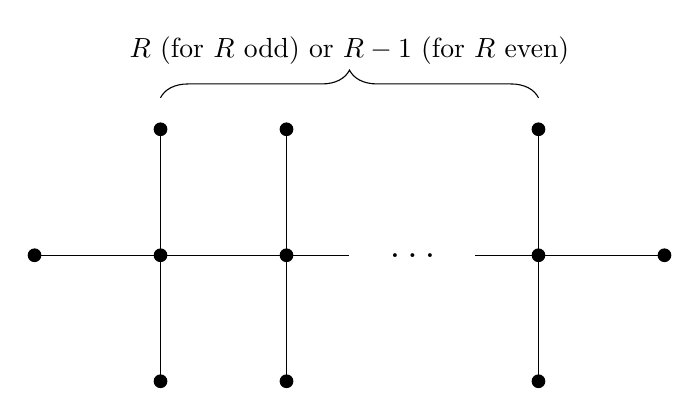
\begin{tikzpicture}[scale=1.6]
\foreach \x in {0,1,2,4,5}
{
  \draw[fill=black,draw=black] (\x cm, 0) circle (.5mm) ;
}
\draw (0,0)--(1,0)--(2,0)--(2.5,0);
\draw (3.5,0)--(4,0)--(5,0);
\node at (3,0) {\Large{$\ldots$}};
\foreach \x in {1,2,4}
{
  \draw[fill=black,draw=black] (\x cm, 1) circle (.5mm) ;
	\draw[fill=black,draw=black] (\x cm, -1) circle (.5mm) ;
	\draw (\x,1)--(\x,0)--(\x,-1);
}
\draw [decorate,decoration={brace,amplitude=10pt}] (1,1.25) -- (4,1.25) node [black,midway,yshift=17]  {$R$ (for $R$ odd) or $R-1$ (for $R$ even)};
\end{tikzpicture}
}
\caption[$G^\triangle$ block representation]{\label{fig:mat_els_for_a_block}}
\end{figure}

For each triple $(z,a,q)$ with $z,a\in\FF_2$ and $q\in[R]$, define
\begin{equation}
  |\phi_{z,a}^{q}\rangle=\begin{cases}
    \frac{1}{\sqrt{3R+2}}\Big[|\psi_{z,a}^{q_{\mathrm{in}}}\rangle+|\psi_{z,a}^{q_{\mathrm{out}}}\rangle+\sum_{j\in[R]}(-1)^j \left(|\psi_{z,a}^{d(q,j)}\rangle-|\psi_{\alpha(q,j),a}^{e_{z0}(q,j)}\rangle-|\psi_{\alpha(q,j),a}^{e_{z1}(q,j)}\rangle\right)\Big] & R\text{ odd}\\
    \frac{1}{\sqrt{3R-1}}\Big[|\psi_{z,a}^{q_{\mathrm{in}}}\rangle+|\psi_{z,a}^{q_{\mathrm{out}}}\rangle+\sum_{j<q}(-1)^j \left(|\psi_{z,a}^{d(q,j)}\rangle-|\psi_{\alpha(q,j),a}^{e_{z0}(q,j)}\rangle-|\psi_{\alpha(q,j),a}^{e_{z1}(q,j)}\rangle\right)\\
       \qquad \qquad \qquad-\sum_{j<q}(-1)^j \left(|\psi_{z,a}^{d(q,j)}\rangle-|\psi_{\alpha(q,j),a}^{e_{z0}(q,j)}\rangle-|\psi_{\alpha(q,j),a}^{e_{z1}(q,j)}\rangle\right)\Big]& R\text{ even.}
  \end{cases}
  \label{eq:phi_z_a_q}
\end{equation}
The choice to omit $d(q,q)$ for $R$ even ensures that $|\psi^{q_{\text{in}}}_{z,a}\rangle$ and $|\psi^{q_{\text{out}}}_{z,a}\rangle$ have the same sign in these ground states, similar to the original gate diagram this gate graph replaced.  We now show that these states span the ground space of $A(G^{\triangle})$.
\begin{lemma}
\label{lem:A(G_triangle)}
An orthonormal basis for the $e_{1}$-energy ground space of $A(G^{\triangle})$ is given by the states
\begin{equation}
  \left\{ |\phi_{z,a}^{q}\rangle:\, z,a\in\{0,1\},\, q\in[R]\right\} 
\end{equation}
defined by equation \eq{phi_z_a_q}. The eigenvalue gap is bounded as 
\begin{equation}
  \gamma(A(G^{\triangle})-e_{1}) > \frac{c_{\triangle}}{R^{2}},
\label{eq:G^triangle_lower_bnd}
\end{equation}
where $c_{\triangle}$ is a constant that only depends on the interaction $\mathcal{U}$.
\end{lemma}

\begin{proof}
The $e_1$-energy ground space of $A(G^{\triangle})$ is equal to the nullspace of \eq{restriction_h_triangle}. Since this operator is block diagonal in the basis $\mathcal{W}$, we can solve for the eigenvectors in the nullspace of each block. Thus, to prove the first part of the lemma, we will analyze the $|\mathcal{W}_{(z,a,q)}|\times|\mathcal{W}_{(z,a,q)}|$ matrix described by \fig{mat_els_for_a_blockA} and show that \eq{phi_z_a_q} is the unique vector in its nullspace. 

We first rewrite the matrix in a slightly different basis obtained by multiplying some of the basis vectors by a phase of $-1$. Specifically, we use the basis
\begin{equation}
\left\{
   |\psi_{z,a}^{q_{\mathrm{in}}}\rangle,
  -|\psi_{z,a}^{d(q,1)}\rangle,
   |\psi_{\alpha(q,1),a}^{e_{z0}(q,1)}\rangle,
   |\psi_{\alpha(q,1),a}^{e_{z1}(q,1)}\rangle,
   |\psi_{z,a}^{d(q,2)}\rangle,
  -|\psi_{\alpha(q,2),a}^{e_{z0}(q,2)}\rangle,
  -|\psi_{\alpha(q,2),a}^{e_{z1}(q,2)}\rangle,
   \ldots,
   |\psi_{z,a}^{q_{\mathrm{out}}}\rangle
\right\} 
\end{equation}
where the state associated with each vertex on one side of a bipartition of the graph is multiplied by $-1$; these are the phases appearing in equation \eq{phi_z_a_q}. Changing to this basis replaces the weight $\frac{1}{8k}$ on each edge in \fig{mat_els_for_a_blockA} by $-\frac{1}{8k}$ and does not change the weights on the self-loops. The resulting matrix is $\frac{1}{8k}L_{0}$, where $L_{0}$ is the Laplacian matrix of the graph shown in \fig{mat_els_for_a_blockB}. 

Now we use the fact that the Laplacian of any connected graph has smallest eigenvalue zero, with a unique eigenvector equal to the all-ones vector.
\todo{Find a citation for this claim}. Hence for each block we get an eigenvector in the nullspace of \eq{restriction_h_triangle}) given by \eq{phi_z_a_q}. Ranging over all $z,a\in\FF_2$ and $q\in[R]$ gives the claimed basis for the $e_1$-energy ground space of $A(G^{\triangle})$.

To prove the lower bound on the eigenvalue gap, we use the Nullspace Projection Lemma (\lem{NPL}) with 
\begin{equation}
H_{A}=A(G^{\diamondsuit})-e_{1}\qquad H_{B}=h_{\mathcal{E}^{\triangle}}
\end{equation}
and where $S=\spn(\mathcal{W})$ is the nullspace of $H_{A}$ as shown in \sec{The-gate-graph_G_DIAMOND}. Since the restriction of $H_B$ to $\mathcal{S}$ is block diagonal in the basis $\mathcal{W}$, the smallest nonzero eigenvalue of \eq{restriction_h_triangle} is equal to the smallest nonzero eigenvalue of one of its blocks. The matrix for each block is $\frac{1}{8k}L_{0}$. Thus we can lower bound the smallest nonzero eigenvalue of $H_B|_S$ using standard bounds on the smallest nonzero eigenvalue of the Laplacian $L$ of a graph $G$. In particular, Theorem 4.2 of reference \cite{Moh91} shows that 
\begin{equation*}
  \gamma(L) \geq \frac{4}{|V(G)| \diam(G)} \geq \frac{4}{|V(G)|^2}
\end{equation*}
(where $\diam(G)$ is the diameter of $G$). Since the size of the graph in \fig{mat_els_for_a_blockB} is either $3R-1$ or $3R+2$, we have
\begin{equation*}
  \gamma(H_{B}|_{S})=\frac{1}{8k}\gamma(L_{0}) \geq \frac{1}{8k}\frac{4}{\left(3R+2\right)^{2}}\geq\frac{1}{32kR^{2}}
\end{equation*}
since $R\geq2$. 

Using this bound and the fact that $\gamma(H_{A})>c_{\diamondsuit}$ (from equation \eq{one_thirteenth_bound}) and $\left\Vert H_{B}\right\Vert =2$ (from equation \eq{h_E_bound}) and plugging into \lem{NPL} gives
\begin{equation}
  \gamma(A(G^{\triangle})-e_{1})\geq\frac{c_{\diamondsuit}\cdot\frac{1}{32kR^{2}}}{c_{\diamondsuit}+2}>\frac{c_{\diamondsuit}}{94 kR^{2}}=\frac{c_{\triangle}}{R^2}. 
\end{equation}
where we used the fact that $c_{\diamondsuit} \leq 1$, and we define $c_\triangle = c_{\diamondsuit}/(96k)$.  As $c_\diamondsuit$ is a constant that only depends on the interaction, so too is $c_\triangle$.
\end{proof}


%=============================================================================
\subsection{The Hamiltonian $H(G^{\triangle},N)$}

With the previous sections results about the graph $G^{\triangle}$, and in particular knowing its ground states and eigenvalue gap, we can now analyze the multi-particle Hamiltonian.  Namely, we can now consider the $N$-particle Hamiltonian $H(G^{\triangle},N)$ and solve for its nullspace. 

In preparation for understanding the $N$-particle states, it will be useful to note the following fact about the subsets $\mathcal{W}_{(z,a,q)}\subset\mathcal{W}$ defined in equation \eq{subset_W}.
\begin{definition}
\label{defn:overlap_diagram_element}
  We say $\mathcal{W}_{(z_{1},a_{1},q_{1})}$ and $\mathcal{W}_{(z_{2},a_{2},q_{2})}$ \emph{overlap in support} if there exist two $l_1,l_2\in L^{\square}$ such that $|\psi_{x_{1},b_{1}}^{l_1}\rangle\in\mathcal{W}_{(z_{1},a_{1},q_{1})}$ and $|\psi_{x_{2},b_{2}}^{l_2}\rangle\in\mathcal{W}_{(z_{2},a_{2},q_{2})}$ for some $x_{1},x_{2},b_{1},b_{2}\in\FF_2$, and either $l_1 = l_2$ or $l_1$ and $l_2$ are adjacent diagram elements.
\end{definition}

\begin{fact}
[Key property of $\mathcal{W}_{(z,a,q)}$]\label{fct:block_property}
Sets $\mathcal{W}_{(z_{1},a_{1},q_{1})}$ and $\mathcal{W}_{(z_{2},a_{2},q_{2})}$ overlap in support if and only if $q_{1}=q_{2}$ or $\{q_{1},q_{2}\}\in E(G^{\text{occ}})$.
\end{fact}
This fact can be confirmed by direct inspection of the sets $\mathcal{W}_{(z,a,q)}$. If $q_{1}=q_{2}=q$ the diagram element $l$ on which they overlap can be chosen to be $l=q_{\mathrm{in}}$; if $q_{1}\neq q_{2}$ and $\{q_{1},q_{2}\}\in E(G^{\text{occ}})$ then $l=e_{z_{1}z_{2}}(q_{1},q_{2})=e_{z_{2}z_{1}}(q_{2},q_{1})$.
Conversely, if $\{q_1,q_2\} \notin E(G^{\text{occ}})$ with $q_1 \ne q_2$, then the two blocks don't have support on the same diagram elements, and in fact the diagram elements supporting the two blocks are separated by at least one additional diagram element (due to the pairwise definitions for the connections between the gate diagrams corresponding to each diagram element of $G$).  This fact is the intuitive reason behind our construction of $G^\square$; we designed the graph $G^\triangle$ so that \fct{block_property} held.

We will show that the nullspace $\mathcal{I}_{\triangle}$ of $H(G^{\triangle},N)$ is 
\begin{align}
  \mathcal{I}_{\triangle}&=\spn\big\{|\phi_{z_{1},a_{1}}^{q_{1}}\rangle|\phi_{z_{2},a_{2}}^{q_{2}}\rangle\ldots|\phi_{z_{N},a_{N}}^{q_{N}}\rangle\colon
\text{$z_{i},a_{i}\in\FF_2$, $q_{i}\in[R]$, $q_{i}\neq q_{j}$, and $\{q_{i},q_{j}\}\notin E(G^{\text{occ}})$}\big\},
\label{eq:I_triangle}
\end{align}
for $\dmax > 0$, and if $\dmax = 0$ we will show that when restricted to symmetric states, the nullspace of $H(G^{\triangle},N)$ is 
\begin{align}
  \mathcal{I}_{\triangle}^{\Sym} &=  \big\{ \Sym ( \ket{\Phi}) \; : \; \ket{\Phi} \in \mathcal{I}_{\triangle}\big\}.
\end{align}
Note that $\mathcal{I}_{\triangle}$ is very similar to $\mathcal{I}(G,G^{\text{occ}},N)$ (from equation \eq{occup_space_defn}) but with each single-particle state $|\psi_{z,a}^{q}\rangle\in\mathcal{Z}_{N}(G)$ replaced by $|\phi_{z,a}^{q}\rangle\in\mathcal{Z}_{N}(G^{\triangle})$ (with the same similarity for the symmetric states).

\todo{Change from $\mathcal{Z}$ to something else}

\begin{lemma}
\label{lem:The-nullspace-of_H_triangle}The nullspace of $H(G^{\triangle},N)$ is $\mathcal{I}_{\triangle}$ as defined in equation \eq{I_triangle} for $\dmax >0$, or when restricted to symmetric states the nullspace of $H(G^\triangle,N)$ is $\mathcal{I}_\triangle^{\Sym}$. In either case, its smallest nonzero eigenvalue is 
\begin{equation}
\gamma(H(G^{\triangle},N)) > \frac{\gamma_{\triangle}}{R^{7}},\label{eq:lowerbound_HG_triangle}
\end{equation}
where $\gamma_{\triangle}$ is a constant that only depends on $\mathcal{U}$.
\end{lemma}

In addition to \fct{block_property}, we use the following simple fact in the proof of the Lemma.

\begin{fact}
\label{fct:lin_alg_fact}
Let $|p\rangle=c|\alpha_{0}\rangle+\sqrt{1-c^{2}}|\alpha_{1}\rangle$ with $\langle\alpha_{i}|\alpha_{j}\rangle=\delta_{ij}$ and $c\in[0,1]$. Then
\begin{equation}
|p\rangle\langle p|=c^{2}|\alpha_{0}\rangle\langle\alpha_{0}|+M
\end{equation}
where $\left\Vert M\right\Vert \leq1-\frac{3}{4}c^{4}$.
\end{fact}

To prove this Fact, one can calculate $\left\Vert M\right\Vert =\frac{1}{2}(1-c^{2})+\frac{1}{2}\sqrt{1+2c^{2}-3c^{4}}$ and use the inequality $\sqrt{1+x}\leq1+\frac{x}{2}$ for $x\geq-1$.

\begin{proof}[Proof of \protect\lem{The-nullspace-of_H_triangle}]  Using equation \eq{A_g_diamond_triangle} and the fact that the smallest eigenvalues of $A(G^{\diamondsuit})$ and $A(G^{\triangle})$ are the same (equal to $e_{1}$, from \sec{The-gate-graph_G_DIAMOND} and \lem{A(G_triangle)}), we can break the MPQW-Hamiltonian on $G^\triangle$ into three terms.  Namely, we have
\begin{equation}
  H(G^{\triangle},N)=H(G^{\diamondsuit},N)+\sum_{w=1}^{N}h_{\mathcal{E}^{\triangle}}^{(w)} + B,\label{eq:H_G^triangle,diamond}
\end{equation}
where $B$ is the change in interaction terms resulting from vertices changing distance.  It is important to realize that $B$ only adds terms to the Hamiltonian, as any vertices that were originally at a distance less than $\dmax$ remain at the same distance when adding the edges in $\mathcal{E}^\triangle$, and thus $B$ is positive semi-definite.  Recall from \lem{The-nullspace-of_Hdiamond} that the nullspace of $H(G^{\diamondsuit},N)$ is $\mathcal{I}_{\diamondsuit}$ (or $\mathcal{I}_\diamondsuit^{\Sym}$ if we are restricting to symmetric states). We consider 
\begin{equation}
  \sum_{w=1}^{N}h_{\mathcal{E}^{\triangle}}^{(w)}\bigg|_{\mathcal{I}_{\diamondsuit}}.\label{eq:restriction to script R}
\end{equation}
We show that its nullspace is equal to $\mathcal{I}_{\triangle}$, and we lower bound its smallest nonzero eigenvalue. Specifically, we prove
\begin{equation}
  \gamma\left(\sum_{w=1}^{N}h_{\mathcal{E}^{\triangle}}^{(w)}\bigg|_{\mathcal{I}_{\diamondsuit}}\right)>\frac{12c_{\triangle}}{(4R)^{6}}.\label{eq:bound_R6}
\end{equation}
Additionally, we will show that $B$ annihilates those states in $\mathcal{I}_{\triangle}$, so that $\mathcal{I}_{\triangle}$ is the nullspace of $H(G^{\triangle},N)$ as claimed.

We will first prove equation \eq{lowerbound_HG_triangle} using this bound on the added movement terms (equation \eq{bound_R6}) and the fact that $B$ annihilates $\mathcal{I}_{\triangle}$. We apply the Nullspace Projection Lemma (\lem{NPL}) with $H_{A}$ and $H_{B}$ given by the first and second terms in equation \eq{H_G^triangle,diamond}; in this case the nullspace of $H_{A}$ is $S=\mathcal{I}_{\diamondsuit}$ (from \lem{The-nullspace-of_Hdiamond}). Now applying \lem{NPL} and using the bounds $\gamma(H_{A})>\gamma_{\diamondsuit}$ (from \lem{The-nullspace-of_Hdiamond}), $\left\Vert H_{B}\right\Vert \leq N\left\Vert h_{\mathcal{E}^{\triangle}}\right\Vert =2N\leq2R$ (from equation \eq{h_E_bound} and the fact that $N\leq R$), and the bound \eq{bound_R6} on $\gamma(H_{B}|_{S})$, we find
\begin{equation}
  \gamma(H(G^{\triangle},N)-B)\geq\frac{\frac{12c_{\triangle}\gamma_{\diamondsuit}}{(4R)^{6}}}{\gamma_{\diamondsuit}+2R}\geq\frac{16 \gamma_{\diamondsuit} c_{\triangle}}{(4R)^7}=\frac{\gamma_\triangle}{R^{7}}.
\end{equation}
If we now use the fact that $B$ annihilates all states in $\mathcal{I}_{\triangle}$, we can use a variational argument to show that the same bound holds for the entire MPQW Hamiltonian (i.e., adding $B$ to the Hamiltonian does not reduce the gap):
\begin{equation}
  \gamma(H(G^{\triangle},N)) \geq \frac{\gamma_{\triangle}}{R^7}.
\end{equation}

With the final reductions for the proof completed, we must now establish that $B$ annihilates all terms in $\mathcal{I}_{\triangle}$, the nullspace of \eq{restriction to script R} is $\mathcal{I}_{\triangle}$, and prove the lower bound \eq{bound_R6}.  Let us first show that each state in $\mathcal{I}_{\triangle}$ has no energy penalty due to new interactions arising from the addition of edges in the graph $G^{\triangle}$.  By definition, note that the only vertices in $G^{\triangle}$ that have vertices at a distance closer than $\dmax$ either belong to the same diagram element, belong to diagram elements corresponding to $\{q_{\text{in}}, q_{\text{out}}, d(q,s)\}$ for some $q\in [R]$, or else belong to diagram elements labeled $\{d(q,s), e_{z_1,z_2}(q,s)\}$ for some $q,s\in [R]$, and $z_1,z_2\in \FF_2$.  As such, if any state has energy penalties resulting from the added edges (i.e., is not annihilated by the operator $B$,), then it must have at least two particles located in two sets $W_{z_1,a_1,q_1}$ and $W_{z_2,a_2,q_2}$ that overlap in support.  However, each state $\ket{\Phi}\in \mathcal{I}_{\triangle}$ is guaranteed by definition to not have any such overlap of support between its several particles, and thus $B\ket{\Phi} = 0$ as required.

To analyze \eq{restriction to script R} we use the fact (established in \sec{The-gate-graph_G_triangle}) that \eq{restriction_h_triangle} is block diagonal with a block $\mathcal{W}_{(z,a,q)}\subset\mathcal{W}$ for each triple $(z,a,q)$ with $z,a\in\FF_2$ and $q\in[R]$, as the operator \eq{restriction to script R} inherits a block structure from this fact. For any basis vector 
\begin{equation}
  |\psi_{z_{1},a_{1}}^{q_{1}}\rangle|\psi_{z_{2},a_{2}}^{q_{2}}\rangle\ldots|\psi_{z_{N},a_{N}}^{q_{N}}\rangle \in\mathcal{I}_{\diamondsuit},
\label{eq:basis_vector_in_scriptF}
\end{equation}
we define a set of occupation numbers that correspond to the number of particles in each block.  Namely, we will define
\begin{equation}
  \mathcal{N}=\left\{ N_{(x,b,r)} \colon x,b\in\{0,1\},\, r\in[R]\right\} 
\end{equation}
where
\begin{equation}
  N_{(x,b,r)}
  =|\{j \colon |\psi_{z_{j},a_{j}}^{q_{j}}\rangle\in\mathcal{W}_{(x,b,r)}\}|.
\end{equation}
Observe that \eq{restriction to script R} conserves the set of occupation numbers (due to the inherited block structure) and is therefore block diagonal with a block for each possible set $\mathcal{N}$. 

(Note that the same definition can be made for the symmetrized states, as we only care about the number of particles in each block.)

For a given block corresponding to a set of occupation numbers $\mathcal{N}$, we write $\mathcal{I}_{\diamondsuit}(\mathcal{N})\subset\mathcal{\mathcal{I}_{\diamondsuit}}$ for the subspace spanned by basis vectors \eq{basis_vector_in_scriptF} in the block. We classify the blocks into three categories depending on $\mathcal{N}$.

\begin{mdframed}[frametitle=Classification of the blocks of \eq{restriction to script R} according to $\mathcal{N}$]
Consider the following two conditions on a set $\mathcal{N}=\{ N_{(x,b,r)}\colon x,b\in\{0,1\},\, r\in[R]\}$
of occupation numbers:
\begin{enumerate}[label=(\alph*)]
\item $N_{(x,b,r)}\in\{0,1\}$ for all $x,b\in\{0,1\}$ and
$r\in[R]$. If this holds, write $\left(y_{i},c_{i},s_{i}\right)$ for the nonzero occupation numbers (with some arbitrary ordering), i.e., $N_{(y_{i},c_{i},s_{i})}=1$ for $i\in[N]$.
\item The sets $\mathcal{W}_{(y_{i},c_{i},s_{i})}$ and $\mathcal{W}_{(y_{j},c_{j},s_{j})}$
do not overlap on a diagram element for all distinct $i,j\in[N]$.
\end{enumerate}
We say a block is of type 1 if $\mathcal{N}$ satisfies (a) and (b). We say it is of type 2 if $\mathcal{N}$ does not satisfy (a). We say it is of type 3 if $\mathcal{N}$ satisfies (a) but does not satisfy (b).
\end{mdframed}


Note that every block must be of type 1, 2, or 3.  We will show that each block of type $1$ contains one state in the nullspace of \eq{restriction to script R} and, ranging over all blocks of this type, we will obtain a basis for $\mathcal{I}_{\triangle}$. We will also show that the smallest nonzero eigenvalue within a block of type 1 is at least $\frac{\gamma_{\diamondsuit}}{R^{2}}$.  We will then show that blocks of type 2 and 3 do not contain any states in the nullspace of \eq{restriction to script R} and that the smallest eigenvalue within any block of type 2 or 3 is greater than $\frac{12c_{\triangle}}{(4R)^6}$. Hence, the nullspace of \eq{restriction to script R} is $\mathcal{I}_{\triangle}$ and its smallest nonzero eigenvalue is lower bounded as in equation \eq{bound_R6}.

%%%%%%%%%%%%%
\smallskip
\noindent \textbf{Type 1}
\smallskip

\noindent Let us first investigate those blocks of type 1.  Note (from \defn{overlap_diagram_element}) that requirement (b) implies $q\neq r$ whenever 
\begin{equation}
|\psi_{x,b}^{q}\rangle\in\mathcal{W}_{(y_{i},c_{i},s_{i})}\text{ and }|\psi_{z,a}^{r}\rangle\in\mathcal{W}_{(y_{j},c_{j},s_{j})}
\end{equation}
for distinct $i,j\in[N]$. Hence, we can remove the requirement that $q_i\neq q_j$:
\begin{align}
  \mathcal{\mathcal{I}_{\diamondsuit}}(\mathcal{N}) 
    & =\spn\{ |\psi_{z_{1},a_{1}}^{q_{1}}\rangle|\psi_{z_{2},a_{2}}^{q_{2}}\rangle\ldots|\psi_{z_{N},a_{N}}^{q_{N}}\rangle\colon q_{i}\neq q_{j}\text{ and } \exists \pi \in S_N , |\psi_{z_{j},a_{j}}^{q_{j}}\rangle\in\mathcal{W}_{(y_{\pi(j)},c_{\pi(j)},s_{\pi(j)})}\} \\
   & =\spn\{|\psi_{z_{1},a_{1}}^{q_{1}}\rangle|\psi_{z_{2},a_{2}}^{q_{2}}\rangle\ldots|\psi_{z_{N},a_{N}}^{q_{N}}\rangle\colon\exists \pi \in S_N ,|\psi_{z_{j},a_{j}}^{q_{j}}\rangle\in\mathcal{W}_{(y_{\pi(j)},c_{\pi(j)},s_{\pi(j)})}\}.
\end{align}
From this we see that 
\begin{equation}
\dim(\mathcal{I}_{\diamondsuit}(\mathcal{N}))
  =(N!)\prod_{j=1}^{N}\left|{\mathcal{W}_{(y_{j},c_{j},s_{j})}}\right|
  =\begin{cases}(
  N!)\left(3R+2\right)^{N} & R\text{ odd}\\
  (N!)\left(3R-1\right)^{N} & R\text{ even.}
\end{cases}
\end{equation}
We now solve for all the eigenstates of \eq{restriction to script R} within the block. (Note that if we restrict to the symmetric subspace, the symmetrization condition simply reduces the size of these subspaces by a factor of $N!$, as the only symmetric state in this subspace is given by the uniform superposition over all these states.)

As we need only understand the eigenvectors of each individual block, it will be useful to remember \lem{A(G_triangle)} as we have already determined all of the single-particle eigenstates.  It will convenient to write an orthonormal basis of eigenvectors of the $|\mathcal{W}_{(z,a,q)}|\times|\mathcal{W}_{(z,a,q)}|$ matrix described by \fig{mat_els_for_a_blockA} as 
\begin{equation}
|\phi_{z,a}^{q}(u)\rangle, \quad u\in[|\mathcal{W}_{(z,a,q)}|]\label{eq:phi_u}
\end{equation}
and their ordered eigenvalues as
\begin{equation}
\theta_{1}\leq\theta_{2}\leq\ldots\leq\theta_{|\mathcal{W}_{(z,a,q)}|}.
\end{equation}
From the proof of \lem{A(G_triangle)}, the eigenvector with smallest eigenvalue $\theta_{1}=0$ is $|\phi_{z,a}^{q}\rangle=|\phi_{z,a}^{q}(1)\rangle$ and $\theta_{2}\geq\frac{c_{\diamondsuit}}{R^{2}}$. For any $u_{1},u_{2},\ldots,u_{N}\in [|\mathcal{W}_{(z,a,q)}|]$, the state 
\begin{equation}
|\phi_{y_{1},c_{1}}^{s_{1}}(u_{1})\rangle|\phi_{y_{2},c_{2}}^{s_{2}}(u_{2})\rangle\ldots|\phi_{y_{N},c_{N}}^{s_{N}}(u_{N})\rangle
\end{equation}
is an eigenvector of \eq{restriction to script R} with eigenvalue $\sum_{j=1}^{N}\theta_{u_j}.$ Furthermore, states corresponding to different choices of $u_{1},\ldots,u_{N}$ are orthogonal, and ranging over all $\dim(\mathcal{I}_{\diamondsuit}(\mathcal{N}))$ choices we get every eigenvector in the block. The smallest eigenvalue within the block is $N\theta_{1}=0$ and there are $N!$ vectors in the nullspace, given by
\begin{equation}
  \ket{\Phi_\mathcal{N}^{\pi}} := |\phi_{y_{\pi(1)},c_{\pi(1)}}^{s_{\pi(1)}}\rangle|\phi_{y_{\pi(2)},c_{\pi(2)}}^{s_{\pi(2)}}\rangle\ldots|\phi_{y_{\pi(N)},c_{\pi(N)}}^{s_{\pi(N)}},\label{eq:vector_type1}
\end{equation}
where $\pi \in S_N$, and where $|\phi_{z,a}^{q}\rangle=|\phi_{z,a}^{q}(1)\rangle$. The smallest nonzero eigenvalue of \eq{restriction to script R} within the block is $(N-1)\theta_{1}+\theta_{2}=\theta_{2}\geq\frac{c_{\diamondsuit}}{R^{2}}$, as expected.  If we restrict ourselves to the symmetric states, this nullspace becomes 1-dimensional, but we still have the same bounds on the eigenvalue gap.

With the knowledge that each state of the form \eq{vector_type1} minimizes the energy of \eq{restriction to script R}, we will now show that the collection of all such states span the space $\mathcal{I}_{\triangle}$.  As the second requirement on type 1 blocks requires that the sets $\mathcal{W}_{(y_i,c_i,s_i)}$ no not pairwise overlap, we can use \fct{block_property} to see that this is equivalent to the sets satisfying $s_{i}\neq s_{j}$ and $\{s_{i},s_{j}\}\notin E(G^{\text{occ}})$ for distinct $i,j\in[N]$ (as well as arbitrary $y_i$ and $c_i$). Hence the set of states \eq{vector_type1} obtained from of all blocks of type 1 is 
\begin{align}
  &\big\{ \ket{\Phi_\mathcal{N}} : \mathcal{N} \text{ is a type 1 block}\big\}\nonumber\\
  &\qquad=\big\{|\phi_{y_{1},c_{1}}^{s_{1}}\rangle|\phi_{y_{2},c_{2}}^{s_{2}}\rangle\ldots|\phi_{y_{N},c_{N}}^{s_{N}}\rangle\colon \nonumber\\
  &\qquad\qquad\qquad\forall i,j\in [N], y_{i},c_{i}\in\FF_2,\, s_{i}\in[R],\, i\neq j \Rightarrow s_{i}\neq s_{j}\text{ and }\,\{s_{i},s_{j}\}\notin E(G^{\text{occ}})\big\} 
\end{align}
which by definition spans $\mathcal{I}_{\triangle}$.  Again, if we restrict ourselves to the symmetric subspace, we also have that these states also span $\mathcal{I}_{\triangle}^{\Sym}$.

\medskip

\noindent \textbf{Type 2}

\smallskip

\noindent Now let $\mathcal{N}$ be of type 2.  We then have that there exist $x,b\in\FF_2$ and $r\in[R]$ such that $N_{(x,b,r)}\geq2$. We will show there are no eigenvectors in the nullspace of \eq{restriction to script R} within a block of this type and we lower bound the smallest eigenvalue within the block. Specifically, we show
\begin{equation}
  \min_{|\kappa\rangle\in\mathcal{I}_{\diamondsuit}(\mathcal{N})}\langle\kappa|\sum_{w=1}^{N}h_{\mathcal{E}^{\triangle}}^{(w)}|\kappa\rangle >\frac{12c_{\triangle}}{(4R)^6}.\label{eq:boundfortype2}
\end{equation}
First note that all $|\kappa\rangle\in\mathcal{I}_{\diamondsuit}$ satisfy $(A(G^{\diamondsuit})-e_{1})^{(w)}|\kappa\rangle=0$ for each $w\in [N]$, which can be seen using the definition of $\mathcal{I}_{\diamondsuit}$ and the fact that $\mathcal{W}$ spans the nullspace of $A(G^{\diamondsuit})-e_{1}$. We can then add these terms to equation \eq{A_g_diamond_triangle}, so that
\begin{equation}
  \min_{|\kappa\rangle\in\mathcal{I}_{\diamondsuit}(\mathcal{N})}\langle\kappa|\sum_{w=1}^{N}h_{\mathcal{E}^{\triangle}}^{(w)}|\kappa\rangle=\min_{|\kappa\rangle\in\mathcal{I}_{\diamondsuit}(\mathcal{N})}\langle\kappa|\sum_{w=1}^{N}\left(A(G^{\triangle})-e_{1}\right)^{(w)}|\kappa\rangle.\label{eq:min_over_blockFbl}
\end{equation}
If we then examine only the ground space of this operator, we can see that
\begin{align}
  \sum_{w=1}^{N}\left(A(G^{\triangle})-e_{1}\right)^{(w)}
  & \geq\gamma\left(\sum_{w=1}^{N}\left(A(G^{\triangle})-e_{1}\right)^{(w)}\right)\cdot
    \left(1-\Pi^{\triangle}\right) \nonumber \\
  &= \gamma(A(G^{\triangle})-e_{1})\cdot\left(1-\Pi^{\triangle}\right)
   > \frac{c_{\triangle}}{R^{2}}\left(1-\Pi^{\triangle}\right),
\label{eq:op_ineq_A_Gtriangle}
\end{align}
where $\Pi^{\triangle}$ is the projector onto the nullspace of $\sum_{w=1}^{N}\left(A(G^{\triangle})-e_{1}\right)^{(w)}$, and where in the last step we used \lem{A(G_triangle)}. Plugging equation \eq{op_ineq_A_Gtriangle} into equation \eq{min_over_blockFbl} gives
\begin{equation}
  \min_{|\kappa\rangle\in\mathcal{I}_{\diamondsuit}(\mathcal{N})}\langle\kappa|\sum_{w=1}^{N}h_{\mathcal{E}^{\triangle}}^{(w)}|\kappa\rangle>\frac{c_{\triangle}}{R^{2}}\Big(1-\max_{|\kappa\rangle\in\mathcal{I}_{\diamondsuit}(\mathcal{N})}\langle\kappa|\Pi^{\triangle}|\kappa\rangle\Big).\label{eq:bound1}
\end{equation}

Using \lem{A(G_triangle)} we can write $\Pi^{\triangle}$ explicitly as
\begin{equation}
\Pi^{\triangle}=\sum_{(\vec{z},\vec{a},\vec{q})\in\mathcal{Q}}\mathcal{P}_{(\vec{z},\vec{a},\vec{q})}\label{eq:Pi_N_triangle}
\end{equation}
where 
\begin{align}
  \mathcal{P}_{(\vec{z},\vec{a},\vec{q})} & =|\phi_{z_{1},a_{1}}^{q_{1}}\rangle\langle\phi_{z_{1},a_{1}}^{q_{1}}|\otimes|\phi_{z_{2},a_{2}}^{q_{2}}\rangle\langle\phi_{z_{2},a_{2}}^{q_{2}}|\otimes\cdots\otimes|\phi_{z_{N},a_{N}}^{q_{N}}\rangle\langle\phi_{z_{N},a_{N}}^{q_{N}}|\\
  \mathcal{Q} & =\left\{ (z_{1},\ldots z_{N},a_{1},\ldots,a_{N},q_{1},\ldots,q_{N}):\, z_{i},a_{i}\in\FF_2\text{ and }q_{i}\in[R]\right\} .
\end{align}
Essentially, each particle is projected onto the ground state of a block, where the blocks are labeled by the elements of $\mathcal{Q}$ and there are no correlations between the particles.  For each $(\vec{z},\vec{a},\vec{q})\in\mathcal{Q}$ we also define a space 
\begin{equation}
  S_{(\vec{z},\vec{a},\vec{q})}=\spn(\mathcal{W}_{(z_{1},a_{1},q_{1})})\otimes\spn(\mathcal{W}_{(z_{2},a_{2},q_{2})})\otimes\cdots\otimes\spn(\mathcal{W}_{(z_{N},a_{N},q_{N})}).
\end{equation}
Note that $\mathcal{P}_{(\vec{z},\vec{a},\vec{q})}$ has all of its support in $S_{(\vec{z},\vec{a},\vec{q})}$, and that
\begin{equation}
S_{(\vec{z},\vec{a},\vec{q})}\perp S_{(\vec{z}^{\prime},\vec{a}^{\prime},\vec{q}^{\prime})}\text{ for distinct }(\vec{z},\vec{a},\vec{q}),(\vec{z}^{\prime},\vec{a}^{\prime},\vec{q}^{\prime})\in\mathcal{Q}.\label{eq:perp_S}
\end{equation}
Therefore $\mathcal{P}_{(\vec{z},\vec{a},\vec{q})}\mathcal{P}_{(\vec{z}^{\prime},\vec{a}^{\prime},\vec{q}^{\prime})}=0$ for distinct $(\vec{z},\vec{a},\vec{q}),(\vec{z}^{\prime},\vec{a}^{\prime},\vec{q}^{\prime})\in\mathcal{Q}$. (Below we use similar reasoning to obtain a less obvious result.) Note that $\mathcal{P}_{(\vec{z},\vec{a},\vec{q})}$ is orthogonal to $\mathcal{I}_{\diamondsuit}(\mathcal{N})$ unless 
\begin{equation}
\left|\left\{ j:(z_{j},a_{j},q_{j})=(w,u,v)\right\} \right|=N_{(w,u,v)}\text{ for all }w,u\in\{0,1\},\, v\in[R].\label{eq:satisfy_occ_numbers}
\end{equation}
We restrict our attention to the projectors that are not orthogonal to $\mathcal{I}_{\diamondsuit}(\mathcal{N})$. Letting $\mathcal{Q}(\mathcal{N})\subset\mathcal{Q}$ be the set of $(\vec{z},\vec{a},\vec{q})$ satisfying equation \eq{satisfy_occ_numbers}, we have
\begin{equation}
\langle\kappa|\sum_{(\vec{z},\vec{a},\vec{q})\in\mathcal{Q}}\mathcal{P}_{(\vec{z},\vec{a},\vec{q})}|\kappa\rangle=\langle\kappa|\sum_{(\vec{z},\vec{a},\vec{q})\in\mathcal{Q}(\mathcal{N})}\mathcal{P}_{(\vec{z},\vec{a},\vec{q})}|\kappa\rangle\quad\text{for all }|\kappa\rangle\in\mathcal{I}_{\diamondsuit}(\mathcal{N}).\label{eq:restrict_attention_mathcalN}
\end{equation}

Since $N_{(x,b,r)}\geq2$, note that in each term $\mathcal{P}_{(\vec{z},\vec{a},\vec{q})}$ with $(\vec{z},\vec{a},\vec{q})\in\mathcal{Q}(\mathcal{N})$, the operator 
\begin{equation}
|\phi_{x,b}^{r}\rangle\langle\phi_{x,b}^{r}|\otimes|\phi_{x,b}^{r}\rangle\langle\phi_{x,b}^{r}|
\end{equation}
appears between two of the $N$ registers (tensored with rank-1 projectors on the other $N-2$ registers). Using equation \eq{phi_z_a_q} we may expand $|\phi_{x,b}^{r}\rangle$ as a sum of states from $\mathcal{W}_{(x,b,r)}$. This gives
\begin{equation}
|\phi_{x,b}^{r}\rangle|\phi_{x,b}^{r}\rangle=c_{0}|\psi_{x,b}^{r_{\text{in}}}\rangle|\psi_{x,b}^{r_{\text{in}}}\rangle+\left(1-c_{0}^{2}\right)^{\frac{1}{2}}|\Phi_{x,b}^{r}\rangle
\end{equation}
where $c_{0}$ is either $\frac{1}{3R+2}$ (if $R$ is odd) or $\frac{1}{3R-1}$ (if $R$ is even), and where $|\psi_{x,b}^{r_{\text{in}}}\rangle|\psi_{x,b}^{r_{\text{in}}}\rangle$ is orthogonal to $|\Phi_{x,b}^{r}\rangle$. Note that each of the states $|\phi_{x,b}^{r}\rangle|\phi_{x,b}^{r}\rangle$, $|\psi_{x,b}^{r_{\text{in}}}\rangle|\psi_{x,b}^{r_{\text{in}}}\rangle$, and $|\Phi_{x,b}^{r}\rangle$ lie in the space 
\begin{equation}
\spn(\mathcal{W}_{(x,b,r)})\otimes\spn(\mathcal{W}_{(x,b,r)}).
\label{eq:tensor_prod_WW}
\end{equation}
Now applying \fct{lin_alg_fact} gives
\begin{equation}
|\phi_{x,b}^{r}\rangle\langle\phi_{x,b}^{r}|\otimes|\phi_{x,b}^{r}\rangle\langle\phi_{x,b}^{r}|=c_{0}^{2}|\psi_{x,b}^{r_{\text{in}}}\rangle\langle\psi_{x,b}^{r_{\text{in}}}|\otimes|\psi_{x,b}^{r_{\text{in}}}\rangle\langle\psi_{x,b}^{r_{\text{in}}}|+M_{x,b}^{r}\label{eq:expand_phi_phi_proj}
\end{equation}
where $M_{x,b}^{r}$ is a Hermitian operator with all of its support on the space \eq{tensor_prod_WW} and
\begin{equation}
\left\Vert M_{x,b}^{r}\right\Vert \leq1-\frac{3}{4}c_{0}^{4}\leq1-\frac{3}{4}\left(\frac{1}{3R+2}\right)^{4}\leq1-\frac{3}{4}\frac{1}{(4R)^4}
\end{equation}
since $R\geq2$. For each $(\vec{z},\vec{a},\vec{q})\in\mathcal{Q}(\mathcal{N})$ we define $\mathcal{P}_{(\vec{z},\vec{a},\vec{q})}^{M}$ to be the operator obtained from $\mathcal{P}_{(\vec{z},\vec{a},\vec{q})}$ by replacing
\begin{equation}
|\phi_{x,b}^{r}\rangle\langle\phi_{x,b}^{r}|\otimes|\phi_{x,b}^{r}\rangle\langle\phi_{x,b}^{r}|\mapsto M_{x,b}^{r}
\end{equation}
on two of the registers (if $N_{(x,b,r)}>2$ there is more than one way to do this; we fix one choice for each $(\vec{z},\vec{a},\vec{q})\in\mathcal{Q}(\mathcal{N})$). Note that $\mathcal{P}_{(\vec{z},\vec{a},\vec{q})}^{M}$ has all of its support in the space $S_{(\vec{z},\vec{a},\vec{q})}$. Using \eq{perp_S} gives
\begin{equation}
\mathcal{P}_{(\vec{z},\vec{a},\vec{q})}^{M}\mathcal{P}_{(\vec{z}^{\prime},\vec{a}^{\prime},\vec{q}^{\prime})}^{M}=0\text{ for distinct }(\vec{z},\vec{a},\vec{q}),(\vec{z}^{\prime},\vec{a}^{\prime},\vec{q}^{\prime})\in\mathcal{Q}(\mathcal{N}).
\end{equation}
Using equation \eq{expand_phi_phi_proj} and the fact that
\begin{equation}
\langle\kappa|\Big(|\psi_{x,b}^{r_{\text{in}}}\rangle\langle\psi_{x,b}^{r_{\text{in}}}|^{(w_{1})}\Big)\Big(|\psi_{x,b}^{r_{\text{in}}}\rangle\langle\psi_{x,b}^{r_{\text{in}}}|^{(w_{2})}\Big)|\kappa\rangle=0\quad\text{for all }|\kappa\rangle\in\mathcal{I}_{\diamondsuit}(\mathcal{N})\text{ and distinct }w_{1},w_{2}\in[N]
\end{equation}
(which can be seen from the definition of $\mathcal{I}_\diamondsuit$), we have 
\begin{equation}
\langle\kappa|\mathcal{P}_{(\vec{z},\vec{a},\vec{q})}|\kappa\rangle=\langle\kappa|\mathcal{P}_{(\vec{z},\vec{a},\vec{q})}^{M}|\kappa\rangle\quad\text{for all }|\kappa\rangle\in\mathcal{I}_{\diamondsuit}(\mathcal{N}).
\end{equation}
Hence, letting 
\begin{equation}
\Pi_{\mathcal{N}}^{\triangle}=\sum_{(\vec{z},\vec{a},\vec{q})\in\mathcal{Q}(\mathcal{N})}\mathcal{P}_{(\vec{z},\vec{a},\vec{q})}^{M},\label{eq:pi_triangle_N}
\end{equation}
we have $\langle\kappa|\Pi^{\triangle}|\kappa\rangle=\langle\kappa|\Pi_{\mathcal{N}}^{\triangle}|\kappa\rangle$ for all $|\kappa\rangle\in\mathcal{I}_{\diamondsuit}(\mathcal{N})$. To obtain a bound on the norm of $\Pi_{\mathcal{N}}^{\triangle}$, we use the fact that the norm of a sum of pairwise orthogonal Hermitian operators is upper bounded by the maximum norm of an operator in the sum, so
\begin{equation}
  \big\Vert \Pi_{\mathcal{N}}^{\triangle}\big\Vert 
    =\Bigg\Vert \sum_{(\vec{z},\vec{a},\vec{q})\in\mathcal{Q}(\mathcal{N})}\mathcal{P}_{(\vec{z},\vec{a},\vec{q})}^{M}\Bigg\Vert 
    =\max_{(\vec{z},\vec{a},\vec{q})\in\mathcal{Q}(\mathcal{N})}\big\Vert \mathcal{P}_{(\vec{z},\vec{a},\vec{q})}^{M}\big\Vert 
    =\left\Vert M_{x,b}^{r}\right\Vert \leq1-\frac{3}{4}\frac{1}{\left(4R\right)^{4}}.
  \label{eq:bound_on_norm_pi_n_triangle}
\end{equation}

Putting this together, we then have that
\begin{equation}
  \max_{\ket{\kappa}\in \mathcal{I}_{\diamondsuit}(\mathcal{N})} \bra{\kappa} \Pi^{\triangle} \ket{\kappa} = \max_{\ket{\kappa}\in \mathcal{I}_{\diamondsuit}(\mathcal{N})} \bra{\kappa} \Pi^{\triangle}_{\mathcal{N}} \ket{\kappa} \leq \norm{\Pi^{\triangle}_{\mathcal{N}}} \leq 1 - \frac{3}{4(4R)^4}.
\end{equation}
If we then use \eq{bound1}, we have that
\begin{equation}
  \min_{|\kappa\rangle\in\mathcal{I}_{\diamondsuit}(\mathcal{N})}\langle\kappa|\sum_{w=1}^{N}h_{\mathcal{E}^{\triangle}}^{(w)}|\kappa\rangle>\frac{c_{\triangle}}{R^{2}}\Big(1-\max_{|\kappa\rangle\in\mathcal{I}_{\diamondsuit}(\mathcal{N})}\langle\kappa|\Pi^{\triangle}|\kappa\rangle\Big) \geq \frac{12c_{\triangle}}{(4R)^6}.
\end{equation}

\medskip

\noindent \textbf{Type 3}

\smallskip

\noindent Let us finally examine the case where $\mathcal{N}$ is of type 3 then $N_{(x,b,r)}\in\{0,1\}$
for all $x,b\in\FF_2$ and $r\in[R]$, and 
\begin{equation}
N_{(y,c,s)}=N_{(t,d,u)}=1
\end{equation}
for some $(y,c,s)\neq(t,d,u)$ with either $u=s$ or $\{u,s\}\in E(G^{\text{occ}})$ (using property (b) and \fct{block_property}). We show there are no eigenvectors in the nullspace of \eq{restriction to script R} within a block of this type and we lower bound the smallest eigenvalue within the block. We establish the same bound \eq{boundfortype2} as for blocks of Type 2.

The proof is very similar to that given above for blocks of Type 2. In fact, the first part of proof is identical, from equation \eq{min_over_blockFbl} up to and including equation \eq{restrict_attention_mathcalN}. That is to say, as in the previous case we have
\begin{equation}
\langle\kappa|\sum_{(\vec{z},\vec{a},\vec{q})\in\mathcal{Q}}\mathcal{P}_{(\vec{z},\vec{a},\vec{q})}|\kappa\rangle=\langle\kappa|\sum_{(\vec{z},\vec{a},\vec{q})\in\mathcal{Q}(\mathcal{N})}\mathcal{P}_{(\vec{z},\vec{a},\vec{q})}|\kappa\rangle\quad\text{for all }|\kappa\rangle\in\mathcal{I}_{\diamondsuit}(\mathcal{N}).\label{eq:restrict_attention_mathcalN-1}
\end{equation}
In this case, since $N_{(y,c,s)}=N_{(t,d,u)}=1$, in each term $\mathcal{P}_{(\vec{z},\vec{a},\vec{q})}$ with $(\vec{z},\vec{a},\vec{q})\in\mathcal{Q}(\mathcal{N})$, the operator 
\begin{equation}
|\phi_{y,c}^{s}\rangle\langle\phi_{y,c}^{s}|\otimes|\phi_{t,d}^{u}\rangle\langle\phi_{t,d}^{u}|
\end{equation}
appears between two of the $N$ registers (tensored with rank 1 projectors on the other $N-2$ registers). Using equation \eq{phi_z_a_q} we may expand $|\phi_{y,c}^{s}\rangle$ and $|\phi_{t,d}^{u}\rangle$ as superpositions (with amplitudes $\pm\frac{1}{\sqrt{3R+2}}$ if $R$ is odd or $\pm\frac{1}{\sqrt{3R-1}}$ if $R$ is even) of the basis states from $\mathcal{W}_{(y,c,s)}$ and $\mathcal{W}_{(t,d,u)}$ respectively. Since $\mathcal{W}_{(y,c,s)}$ and $\mathcal{W}_{(t,d,u)}$ overlap on some diagram element, there exists $l\in L^{\square}$ such that $|\psi_{x_{1},b_{1}}^{l}\rangle\in\mathcal{W}_{(y,c,s)}$ and $|\psi_{x_{2},b_{2}}^{l}\rangle\in\mathcal{W}_{(t,d,u)}$ for some $x_{1},x_{2},b_{1},b_{2}\in\{0,1\}$. Hence
\begin{equation}
|\phi_{y,c}^{s}\rangle|\phi_{t,d}^{u}\rangle=c_{0}\left(\pm|\psi_{x_{1},b_{1}}^{l}\rangle|\psi_{x_{2},b_{2}}^{l}\rangle\right)+\left(1-c_{0}^{2}\right)^{\frac{1}{2}}|\Phi_{y,c,t,d}^{s,u}\rangle
\end{equation}
where $c_{0}$ is either $\frac{1}{3R+2}$ (if $R$ is odd) or $\frac{1}{3R-1}$ (if $R$ is even). Now applying \fct{lin_alg_fact} we get
\begin{equation}
|\phi_{y,c}^{s}\rangle\langle\phi_{y,c}^{s}|\otimes|\phi_{t,d}^{u}\rangle\langle\phi_{t,d}^{u}|=c_{0}^{2}|\psi_{x_{1},b_{1}}^{l}\rangle\langle\psi_{x_{1},b_{1}}^{l}|\otimes|\psi_{x_{2},b_{2}}^{l}\rangle\langle\psi_{x_{2},b_{2}}^{l}|+M_{y,c,t,d}^{s,u}\label{eq:expand_phi_phi_proj-1-1}
\end{equation}
where $\Vert M_{y,c,t,d}^{s,u}\Vert \leq1-\frac{3}{4}\left(\frac{1}{4R}\right)^{4}$. For each $(\vec{z},\vec{a},\vec{q})\in\mathcal{Q}(\mathcal{N})$ we define $\mathcal{P}_{(\vec{z},\vec{a},\vec{q})}^{M}$ to be the operator obtained from $\mathcal{P}_{(\vec{z},\vec{a},\vec{q})}$ by replacing
\begin{equation}
|\phi_{y,c}^{s}\rangle\langle\phi_{y,c}^{s}|\otimes|\phi_{t,d}^{u}\rangle\langle\phi_{t,d}^{u}|\mapsto M_{y,c,t,d}^{s,u}
\end{equation}
on two of the registers and we let $\Pi_{\mathcal{N}}^{\triangle}$ be given by \eq{pi_triangle_N}. Then, as in the previous case, $\langle\kappa|\Pi^{\triangle}|\kappa\rangle=\langle\kappa|\Pi_{\mathcal{N}}^{\triangle}|\kappa\rangle$ for all $|\kappa\rangle\in\mathcal{I}_{\diamondsuit}(\mathcal{N})$ and using the same reasoning as before, we get the bound \eq{bound_on_norm_pi_n_triangle} on $\Vert \Pi_{\mathcal{N}}^{\triangle}\Vert $. Using these two facts we get the same bound on the smallest eigenvalue within a block of type 3 as the bound we obtained for blocks of type 2:
\begin{align}
\min_{|\kappa\rangle\in\mathcal{I}_{\diamondsuit}(\mathcal{N})}\langle\kappa|\sum_{w=1}^{N}h_{\mathcal{E}^{\triangle}}^{(w)}|\kappa\rangle &>\frac{c_{\triangle}}{R^{2}}\Big(1-\max_{|\kappa\rangle\in\mathcal{I}_{\diamondsuit}(\mathcal{N})}\langle\kappa|\Pi^{\triangle}|\kappa\rangle\Big) \geq \frac{12c_{\triangle}}{(4R)^6}.\qedhere
\end{align}
\end{proof}

%=============================================================================
\subsection{The gate graph $G^{\square}$ }

With all of the intermediate graphs characterized, we now consider the gate graph $G^{\square}$ and prove \lem{oc}. We first show that $G^{\square}$ is an $e_{1}$-gate graph. From equations \eq{A_G_squAre}, \eq{h_se_square}, and \eq{A_g_triangle} we have
\begin{equation}
A(G^{\square})=A(G^{\triangle})+h_{\mathcal{E}^{0}}+h_{\mathcal{S}^{0}}.\label{eq:A_g_square_triangle}
\end{equation}
\lem{A(G_triangle)} characterizes the $e_{1}$-energy ground space of $G^{\triangle}$ and gives an orthonormal basis for it. To solve for the $e_{1}$-energy ground space of $A(G^{\square})$, we solve for superpositions of the ground states of $A(G^\triangle)$,  $\{|\phi_{z,a}^{q}\rangle\}$, in the nullspace of $h_{\mathcal{E}^{0}}+h_{\mathcal{S}^{0}}$.

Recall the definition of the sets $\mathcal{E}^{0}$ and $\mathcal{S}^{0}$, as these are the edges and self-loops that are inherited from the graph $G$. From \sec{g_square_def}, each node $(q,z,t)$ in the gate diagram for $G$ is associated with a node $\new(q,z,t)$ in the gate diagram for $G^{\square}$ as described by \eq{node_mapping_G_G_square}. This mapping is depicted in \fig{replace_gate_diagram} by the black and grey arrows. Applying this mapping to each pair of nodes in the edge set $\mathcal{E}^{G}$ and each node in the self-loop set $\mathcal{S}^{G}$ of the gate diagram for $G$, we get the sets $\mathcal{E}^{0}$ and $\mathcal{S}^{0}$. Hence, using equations \eq{h_loops} and \eq{h_edges},
\begin{align}
h_{\mathcal{S}^0} &=\sum_{(q,z,t)\in \mathcal{S}^G} |{\new(q,z,t)}\rangle\langle{\new(q,z,t)}|\otimes \II \label{eq:hS0}\\
h_{\mathcal{E}^0} &=\sum_{\{(q,z,t),(q^\prime,z^\prime,t^\prime)\}\in \mathcal{E}^G} \left(|{\new(q,z,t)}\rangle+|{\new(q^\prime,z^\prime,t^\prime)}\rangle\right)\left(\langle{\new(q,z,t)}|+\langle{\new(q^\prime,z^\prime,t^\prime)}|\right)\otimes \II.\label{eq:hE0}
\end{align}

Using equation \eq{phi_z_a_q}, we see that for all nodes $(q,z,t)$ in the gate diagram for $G$ and for all $j\in[8]$, $x,b,d\in\FF_2$, and $r\in[R]$,
\begin{align}
  \langle{\new(q,z,t),j,d}|\phi^r_{x,b}\rangle & =\sqrt{c_0}
    \begin{cases}
      \langle q_{\mathrm{in}},z,t,j,d|\psi^{r_{\mathrm{in}}}_{x,b}\rangle & \text{ if $(q,z,t)$ is an input node}\\
      \langle q_{\mathrm{out}},z,t,j,d|\psi^{r_{\mathrm{out}}}_{x,b}\rangle & \text{ if $(q,z,t)$ is an output node}
    \end{cases}\nonumber \\
  &=\sqrt{c_0}\delta_{r,q} \langle z,t,j,d|\overline{\psi_{x,b}}\rangle
  \label{eq:mat_el_newnodes}
\end{align}
where $c_0$ is $\frac{1}{3R+2}$ if $R$ is odd or $\frac{1}{3R-1}$ if $R$ is even, and where $|\psi_{x,b}\rangle$ is defined by equations \eq{psi0m} and \eq{psi1m}. The matrix element on the left-hand side of this equation is evaluated in the Hilbert space $\CC^{|V(G^\square)|}$ where each basis vector corresponds to a vertex of the graph $G^\square$; these vertices are labeled $(l,z,t,j,d)$ with $l\in L^\square$, $z,d\in \FF_2$, $t\in[8k]$, and $j\in[8]$. However, from \eq{mat_el_newnodes} we see that
\begin{equation}
  \underbrace{\langle \new(q,z,t),j,d|\phi^r_{x,b}\rangle}_{\text{in } \mathcal{Z}_1 (G^\square)}=\sqrt{c_0}\underbrace{\langle q,z,t,j,d|\psi^r_{x,b}\rangle}_{\text{in } \mathcal{Z}_1 (G)} \label{eq:twoHspaces}
\end{equation}
where the right-hand side is evaluated in the Hilbert space $\CC^{|V(G)|}$.

Putting together equations \eq{hS0}, \eq{hE0}, and \eq{twoHspaces} gives
\begin{equation}
  \langle\phi_{z,a}^{q}|h_{\mathcal{E}^{0}}+h_{\mathcal{S}^{0}}|\phi_{x,b}^{r}\rangle=\langle\psi_{z,a}^{q}|h_{\mathcal{E}^{G}}+h_{\mathcal{S}^{G}}|\psi_{x,b}^{r}\rangle\cdot
  \begin{cases}
    \frac{1}{3R+2} & R\text{ odd}\\
    \frac{1}{3R-1} & R\text{ even}
  \end{cases}
  \label{eq:h_eG_hsG}
\end{equation}
for all $z,a,x,b\in\FF_2$ and $q,r\in[R]$. 

We use equation \eq{h_eG_hsG} to relate the $e_1$-energy ground states of $A(G)$ to those of $A(G^\square)$. Since $G$ is an $e_{1}$-gate graph, there is a state 
\begin{equation}
  |\Gamma\rangle=\sum_{z,a,q}\alpha_{z,a,q}|\psi_{z,a}^{q}\rangle\in\CC^{|V(G)|}
\end{equation}
that satisfies $A(G)|\Gamma\rangle=e_1|\Gamma\rangle$ and hence $h_{\mathcal{E}^{G}}|\Gamma\rangle=h_{\mathcal{S}^{G}}|\Gamma\rangle=0$. Letting
\begin{equation}
  |\Gamma^{\prime}\rangle=\sum_{z,a,q}\alpha_{z,a,q}|\phi_{z,a}^{q}\rangle\in\CC^{|V(G^\square)|}
\end{equation}
and using equation \eq{h_eG_hsG}, we see that $\langle\Gamma^{\prime}|h_{\mathcal{E}^{0}}+h_{\mathcal{S}^{0}}|\Gamma^{\prime}\rangle=0$ and therefore $\langle\Gamma^{\prime}|A(G^{\square})|\Gamma^{\prime}\rangle=e_{1}$. Hence $G^{\square}$ is an $e_{1}$-gate graph. Moreover, the linear mapping from $\CC^{|V(G)|}$ to $\CC^{|V(G^\square)|}$ defined by
\begin{equation}
  |\psi_{z,a}^{q}\rangle \mapsto |\phi_{z,a}^{q}\rangle\label{eq:map_1particle}
\end{equation}
maps each $e_{1}$-energy eigenstate of $A(G)$ to an $e_{1}$-energy eigenstate of $A(G^{\square})$.

Now consider the $N$-particle Hamiltonian $H(G^{\square},N)$. Using equation \eq{A_g_square_triangle} and the fact that both $A(G^{\square})$ and $A(G^{\triangle})$ have smallest eigenvalue $e_{1}$, we have
\begin{equation}
  H(G^{\square},N)=H(G^{\triangle},N)+\sum_{w=1}^{N}\left(h_{\mathcal{E}^{0}}+h_{\mathcal{S}^{0}}\right)^{(w)}\bigg|_{\mathcal{Z}_{N}(G^{\square})} + C',
\end{equation}
where $C$ corresponds to the added interactions resulting from the additional edges. Recall from \lem{A(G_triangle)} that the nullspace of the first term is $\mathcal{I}_{\triangle}$. The $N$-fold tensor product of the mapping \eq{map_1particle} acts on basis vectors of $\mathcal{I}(G,G^{\text{occ}},N)$ as 
\begin{equation}
  |\psi_{z_{1},a_{1}}^{q_{1}}\rangle|\psi_{z_{2},a_{2}}^{q_{2}}\rangle\ldots|\psi_{z_{N},a_{N}}^{q_{N}}\rangle
    \mapsto
  |\phi_{z_{1},a_{1}}^{q_{1}}\rangle|\phi_{z_{2},a_{2}}^{q_{2}}\rangle\ldots|\phi_{z_{N},a_{N}}^{q_{N}}\rangle,
  \label{eq:N_particle_mapping}
\end{equation}
where $z_{i},a_{i}\in\FF_2,\; q_{i}\neq q_{j},\;\text{and }\{q_{i},q_{j}\}\notin E(G^{\text{occ}})$.
Clearly this defines an invertible linear map between the two spaces
$\mathcal{I}(G,G^{\text{occ}},N)$ and $\mathcal{I}_{\triangle}$. Let $|\Theta\rangle\in\mathcal{I}(G,G^{\text{occ}},N)$
and write $|\Theta^{\prime}\rangle\in\mathcal{I}_{\triangle}$ for its image under the map \eq{N_particle_mapping}. Then 
\begin{align}
  \langle\Theta^{\prime}|H(G^{\square},N)-C'|\Theta^{\prime}\rangle&=\langle\Theta^{\prime}|\sum_{w=1}^{N}\left(h_{\mathcal{E}^{0}}+h_{\mathcal{S}^{0}}\right)^{(w)}|\Theta^{\prime}\rangle\\
  &=\langle\Theta|\sum_{w=1}^{N}\left(h_{\mathcal{E}^{G}}+h_{\mathcal{S}^{G}}\right)^{(w)}|\Theta\rangle\cdot
  \begin{cases}
    \frac{1}{3R+2} & R\text{ odd}\\
    \frac{1}{3R-1} & R\text{ even}
  \end{cases}
\label{eq:Theta_Theta_prime_eqn}
\end{align}
where in the first equality we used the fact that $|\Theta^\prime\rangle$ is in the nullspace $\mathcal{I}_{\triangle}$ of $H(G^\triangle,N)$ and in the second equality we used equation \eq{h_eG_hsG} and the fact that $\langle\phi_{z,a}^{q}|\phi_{x,b}^{r}\rangle=\langle\psi_{z,a}^{q}|\psi_{x,b}^{r}\rangle$. 

We now want to understand how $C'$ changes the ground space along with the eigenvalue gap.  While the added edges will add energy to those states on $G^\square$ if and only if they add energy to the corresponding state on $G$ that also satisfy the occupancy constraints, the fact that the states on $G^\square$ are much more spread out means that the added energy can be drastically less.  In particular, an arbitrary state on $G$ might have $N$-particle interactions which under our transformation would require a factor of $(3R)^{-N}$ to the energy.  However, the fact that each state in $\mathcal{I}_{\triangle}$ and each state in $\mathcal{I}(G,G^{\text{occ}},N)$ satisfy the occupancy constraints implies that at most a single particle ever occupies a single diagram element (and thus $C'=0$ if $\dmax = 0$).  Using this, we have that when restricted to those states in $\mathcal{I}_{\triangle}$, each term in $C'$ affects at most two particles, and  the requisite change to the energy penalty will only be $(3R)^{-2}$.

As such, let $u'$ and $v'$ be two vertices of $G^\square$ that can now interact but were separated by a distance more than $\dmax$ in $G^\triangle$.  We can see that each such vertex is contained within some diagram element $q_{\text{in}}$ or $q_{\text{out}}$.  Further, each pair $(u',v')$ of vertices in $G^\square$ for which interactions are added has a corresponding pair of vertices $(u,v)$ in $G$ for which the interactions were also added, derived by simply dropping the in/out from the label for the diagram element.  Similarly, for any two vertices $(u,v)$ in $G$ for which the added edges cause an interaction, there exist two vertices $(u',v')$ in $G^\square$ that also have an interaction, which can be found by adding in the in/out to the diagram element labels for $u$ and $v$, depending where the edge that connects the two diagram elements is located (i.e., whether it connects to the input or output of the element).  Since this is a bijection between pairs of vertices (but not individual vertices), we will have that the added interactions will be proportional between those states in $\mathcal{I}_{\triangle}$ and $\mathcal{I}(G,G^{\text{occ}},N)$.  We will let $V^\square \subset V(G^\square) \times V(G^\square)$ be those vertices in $G^\square$ that are now at a distance less than or equal to $\dmax$ that were farther apart than $\dmax$ in $G^\triangle$, and let $V\subset V(G)\times V(G)$ be the corresponding pairs of vertices in $G$.

Explicitly, note that for any pair of vertices $(u',v')\in V^\square$ that are now a distance $d$, and any state $\ket{\Theta'} \in \mathcal{I}(G^\triangle,N)$,
\begin{align}
  \bra{\Theta'}\mathcal{U}_d(\hat{n}_{u'},\hat{n}_{v'}) \ket{\Theta'} &= U_{d}^{(1,1)}\sum_{w_1\neq w_2\in[N]} \bra{\Theta'}\big(\ketbra{u'}{u'}^{(w_1)} \otimes \ketbra{v'}{v'}^{(w_2)}\big) \ket{\Theta'}\\
  & =U_{d}^{(1,1)}\sum_{w_1\neq w_2\in[N]} \bra{\Theta}\big(\ketbra{u}{u}^{(w_1)} \otimes \ketbra{v}{v}^{(w_2)}\big) \ket{\Theta} \begin{cases}
       \frac{1}{(3R+2)^2} & R\text{ odd}\\
       \frac{1}{(3R-1)^2} & R\text{ even}
    \end{cases}\\
  &= \bra{\Theta} \mathcal{U}_d( \hat{n}_u,\hat{n}_v) \ket{\Theta}\begin{cases}
       \frac{1}{(3R+2)^2} & R\text{ odd}\\
       \frac{1}{(3R-1)^2} & R\text{ even}.
    \end{cases}
\end{align}
This uses a relation almost identical to \eq{mat_el_newnodes}, which can be derived in an identical manner.

With this identity in mind, we have that 
\begin{align}
  \bra{\Theta'} C' \ket{\Theta'} &= \sum_{(u',v')\in \mathcal{V}^\square} \bra{\Theta'}\mathcal{U}_{d(u',v')}(\hat{n}_{u'},\hat{n}_{v'}) \ket{\Theta'} \\
   &= \sum_{(u,v)\in \mathcal{V}} \bra{\Theta} \mathcal{U}_{d(u,v)}( \hat{n}_u,\hat{n}_v) \ket{\Theta}\begin{cases}
       \frac{1}{(3R+2)^2} & R\text{ odd}\\
       \frac{1}{(3R-1)^2} & R\text{ even}.
    \end{cases}\\
  &= \bra{\Theta} C \ket{\Theta} \begin{cases}
       \frac{1}{(3R+2)^2} & R\text{ odd}\\
       \frac{1}{(3R-1)^2} & R\text{ even}
    \end{cases}
    \label{eq:C' relation}
\end{align}

We now complete the proof of \lem{oc} using equation \eq{Theta_Theta_prime_eqn} and \eq{C' relation}.

%-----------------------------------------------------------------------------
\subsubsection*{Case 1: $\lambda_{N}(G,G^{\text{occ}})\leq a$}

In this case there exists a state $|\Theta\rangle\in\mathcal{I}(G,G^{\text{occ}},N)$ satisfying 
\begin{equation}
\langle\Theta|\sum_{w=1}^{N}\left(h_{\mathcal{E}^{G}}+h_{\mathcal{S}^{G}}\right)^{(w)} + C|\Theta\rangle = a_{\text{adj}} + a_\text{int}\leq a,
\end{equation}

From equation \eq{Theta_Theta_prime_eqn} we see that the state $|\Theta^{\prime}\rangle\in\mathcal{I}_{\triangle}$ satisfies $\langle\Theta^{\prime}|\Theta^{\prime}\rangle\leq\frac{a_{\text{adj}}}{3R-1}$, and from $\eq{C' relation}$ that it also satisfies $\bra{\Theta'} C' \ket{\Theta'} \leq \frac{a_{\text{int}}}{(3R-1)^2}$.

Putting this together, (along with the fact that $\ket{\Theta'}\in \mathcal{I}_{\triangle}$ and thus is in the nullspace of $H(G^{\triangle},N)$),
\begin{equation}
  \bra{\Theta'}H(G^{\square},N) \ket{\Theta'} \leq \frac{a_{\text{adj}}}{3R-1} + \frac{a_{\text{int}}}{(3R-1)^2} < \frac{a_{\text{adj}}}{R} + \frac{a_{\text{int}}}{R} = \frac{a}{R}.
\end{equation}

%-----------------------------------------------------------------------------
\subsubsection*{Case 2: $\lambda_{N}(G,G^{\text{occ}})\geq b$}

In this case 
\begin{align}
\lambda_{N}(G,G^{\text{occ}})&=\min_{|\Theta\rangle\in\mathcal{I}(G,G^{\text{occ}},N)}\langle\Theta|H(G,G^{\text{occ}},N)|\Theta\rangle\\
   & = \min_{|\Theta\rangle\in\mathcal{I}(G,G^{\text{occ}},N)}\langle\Theta|\sum_{w=1}^{N}\left(h_{\mathcal{E}^{G}}+h_{\mathcal{S}^{G}}\right)^{(w)}|\Theta\rangle + \bra{\Theta} C \ket{\Theta}\\
   &= b_{\text{adj}} + b_{\text{int}} \geq  b.
\end{align}
 Now applying equation \eq{Theta_Theta_prime_eqn} and \eq{C' relation} gives
\begin{align}
  \min_{|\Theta^{\prime}\rangle\in\mathcal{I}_{\triangle}}\langle\Theta^{\prime}|H(G^{\square},N)|\Theta^{\prime}\rangle&=\min_{|\Theta^{\prime}\rangle\in\mathcal{I}_{\triangle}}\langle\Theta^{\prime}|\sum_{w=1}^{N}\left(h_{\mathcal{E}^{0}}+h_{\mathcal{S}^{0}}\right)^{(w)}|\Theta^{\prime}\rangle + \bra{\Theta'} C' \ket{\Theta'}\\
  &= \frac{b_{\text{adj}}}{3R+2} + \frac{b_{\text{int}}}{(3R+2)^2}\\
  &\geq\frac{1}{(3R+2)^2}b,\label{eq:bound_thetaprime}
\end{align}
This establishes that the nullspace of $H(G^{\square},N)$ is empty, i.e., $\lambda_{N}^{1}(G^{\square})>0$, so $\lambda_{N}^{1}(G^{\square})=\gamma(H(G^{\square},N))$. We lower bound $\lambda_{N}^{1}(G^{\square})$ using the Nullspace Projection Lemma (\lem{NPL}) with
\begin{equation}
  H_{A}=H(G^{\triangle},N)\qquad H_{B}=\sum_{w=1}^{N}\left(h_{\mathcal{E}^{0}}+h_{\mathcal{S}^{0}}\right)^{(w)}\bigg|_{\mathcal{Z}_{N}(G^{\square})} + C'
\end{equation}
and where the nullspace of $H_{A}$ is $S=\mathcal{I}_{\triangle}$. We apply \lem{NPL} and use the bounds $\gamma(H_{A})>\frac{\gamma_\triangle}{R^{7}}$ (from \lem{The-nullspace-of_H_triangle}), $\gamma(H_{B}|_{S})\geq\frac{b}{(3R+2)^2}$ (from equation \eq{bound_thetaprime}), and 
\begin{equation}
  \left\Vert H_{B}\right\Vert \leq N\left\Vert {h_{\mathcal{E}^{0}}+h_{\mathcal{S}^{0}}}\right\Vert  + \norm{H_{\text{int}}} \leq3N + d_{\mathcal{U}} N^{\nu}
  \leq d_{\mathcal{U}}R^{\nu_\mathcal{U}}
\end{equation}
(using equations \eq{h_E_bound} and \eq{h_S_bound}, the bounds on $H_{\text{int}}$, and the fact that $N\leq R$) to find 
\begin{align}
\lambda_{N}^{1}(G^{\square}) &= \gamma(H(G^{\square},N)) \\
 &\geq \frac{\gamma_{\triangle}b}{(3R+2)^2R^7}\frac{1}{\frac{\gamma_{\triangle}}{R^7}+d_{\mathcal{U}} R^{\nu_{\mathcal{U}}}} \\
 & >\frac{ \gamma_{\square} b}{R^{9+\nu}}
\end{align}
where $\gamma_{\square}$ depends only on the interaction $\mathcal{U}$, and we have our requisite bound.


%%%%%%%%%%%%%%%%%%%%%%%%%%%%%%%%%%%%%%%%%%%%%%%%%
\section{Constructing the graph for a given circuit}\label{sec:graph_construction}

In order to prove that bounding the ground energy of a MPQW on some graph $G_X$ is as hard as bounding the maximal acceptance probability of a circuit $\mathcal{C}_X$, we will need to somehow relate the ground energy of $G_X$ to the maximal acceptance probability for the circuit $\mathcal{C}_X$.  

With the graphs defined in \sec{graph_primitives} and the ability to ensure that certain states are excluded from the ground space via the occupancy constraints lemma \sec{occupancy_constraints}, we will be able to do this.   In particular, we will show how to transform a circuit with a given form into a graph, such that the $n$-particle ground-energy will correspond to whether the circuit has an accepting state when certain states are excluded from the ground space.  

The main idea will be to use the graph primitives of \sec{graph_primitives} to replace each gate from $\mathcal{C}_X$ with a particular gadget. By using a single particle for each qubit, and forcing each unitary to affect the first qubit, we will be able to use the location of the first particle to encode the current ``time'' of the occupation.  Using our two-particle graph gadgets, we can then ensure that the particles move together through the entire computation (assuming that they start in the correct positions).  

This construction is somewhat complicated, but we will define the graph $G_X$ and the necessary occupancy constraints in this section.  We will then prove the bound relating the acceptance probability of the circuit to the smallest eigenvalue (with the occupancy constraints) in \sec{g_x_proof}.

\subsection{Verification circuits} \label{sec:verification_circuit}

We take the verification circuit $\mathcal{C}_{X}$ that we want to simulate to be from the following universal circuit family.  We will assume that $\mathcal{C}_X$ acts on $n\geq 4$ qubits and has $M$ total gates
\begin{align}
  U_{\mathcal{C}_{X}}=U_{M}U_{M-1}\ldots U_{1},
\end{align}
where each gate $U_j$ is a two-qubit gate acting nontrivially on the qubit labeled $1$ and another qubit $s(j)\in\{2,\ldots,n\}$, and is chosen from the set
\begin{equation}
  \{\CNOT_{1s(j)},\CNOT_{s(j)1},\CNOT_{1s(j)}\left(H\otimes\II\right),\CNOT_{1s(j)}\left(HT\otimes\II\right)\}.\label{eq:gate_set_Vr}
\end{equation}
Additionally, we will assume that no two consecutive gates ($U_j$ and $U_{j+1}$) act between the same two qubits, i.e., 
\begin{equation}
s(j)\neq s(j+1)\qquad j\in[M-1],\label{eq:condition_ij}
\end{equation}
and we assume that each qubit be involved in at least one gate.

We will think of the input state to the circuit being given to us on the qubits labeled $1,\ldots,n_{\text{in}}$, while the remaining $n-n_{\text{in}}$ qubits are each initialized to $|0\rangle$ and are used as ancilla.  We will assume that the output of the circuit is contained in the state of the second qubit, as the first mediates all of the other interactions.

Note that the acceptance probability for the circuit acting on input state $|\psi_{{\text{in}}}\rangle\in(\CC^{2})^{\otimes n_{{\text{in}}}}$ is the probability that a final measurement of the output qubit in the computational basis gives the value $1$: 
\begin{align}
\AP\left(\mathcal{C}_{X},|\psi_{{\text{in}}}\rangle\right)=\left\Vert |1\rangle\langle1|^{(2)}U_{\mathcal{C}_{X}}|\psi_{{\text{in}}}\rangle|0\rangle^{\otimes n-n_{{\text{in}}}}\right\Vert ^{2},
\end{align}
and thus we will eventually want to ensure that the final state of qubit 2 to be 1.

We will now establish that circuits of this form are universal. We show that any quantum circuit (with $n\geq 4$ qubits) expressed using the universal gate set
\begin{equation}
\{\CNOT,H,HT\}\label{eq:standard_gate_ste}
\end{equation}
can be efficiently rewritten in the prescribed form without increasing the number of qubits and with at most a constant factor increase in the number of gates.

First we map a circuit from the gate set \eq{standard_gate_ste} to the gate set \eq{gate_set_Vr} (without necessarily satisfying condition \eq{condition_ij}). A $\SWAP$ gate between qubits $1$ and $k$ can be performed using the identity
\begin{align}
  \SWAP_{1k} & = \CNOT_{1k}\CNOT_{k1}\CNOT_{1k}.
\end{align}
To perform a $\CNOT_{ik}$ gate between two qubits $i,k$ (neither of which is qubit $1$), we swap qubits $1$ and $i$, apply $\CNOT_{1k}$, and then swap back. Similarly, we can apply a single-qubit gate $U\in\{H,HT\}$ to some qubit $k\neq1$ using the sequence of gates
\begin{align}
  \SWAP_{1k} \CNOT_{12} \left(\CNOT_{12} U\otimes\II\right) \SWAP_{1k}.
\end{align}
Applying these replacement rules, we obtain a circuit over the gate set \eq{gate_set_Vr}. However, the resulting circuit will not in general satisfy equation \eq{condition_ij}. To enforce this condition, we insert a sequence of four gates equal to the identity, namely
\begin{align}
  \II=\CNOT_{1a}\CNOT_{1b}\CNOT_{1a}\CNOT_{1b},
\end{align}
between any two consecutive gates $U_j$ and $U_{j+1}$ with $s(j)=s(j+1)$, where $a\neq b \neq s(j)$. For example, 
\begin{align}
\CNOT_{15}\CNOT_{51}\quad\longrightarrow\quad\CNOT_{15}\CNOT_{12}\CNOT_{13}\CNOT_{12}\CNOT_{13}\CNOT_{51}.
\end{align}
Thus we map any circuit over the gate set \eq{standard_gate_ste} into the prescribed form. Note that $n\geq 4$ is needed to ensure that any quantum circuit can be efficiently rewritten so that $s(j) \neq s(j+1)$.  There do exist circuits with $n=3$ for which our construction works, such as the example shown in \fig{step-by-step}.

%%%%%%%%%%%%%%%%%%%%%%%%
\subsection{Gate graph for a given circuit}\label{sec:g_x_defn}
For any $n$-qubit, $M$-gate verification circuit $\mathcal{C}_{X}$ of the form described in \sec{verification_circuit}, we associate a gate graph $G_X$. The gate diagram for $G_X$ is built using the gadgets described in \sec{graph_primitives}; specifically, we use $M$ two-qubit gadgets and $2(n-1)$ boundary gadgets. Since each two-qubit gadget and each boundary gadget contains $88$ diagram elements, the total number of diagram elements in $G_X$ is $R=88(M+2n-2)$.


\todo{fix this paragraph}
We now present the construction of the gate diagram for $G_X$.  We also describe some gate graphs obtained as intermediate steps that are used in our analysis in \sec{Proof-of-Theorem}. The reader may find this description easier to follow by looking ahead to \fig{step-by-step}, which illustrates this construction for a specific $3$-qubit circuit.

\begin{enumerate}
  \item \textbf{Draw a grid} with columns labeled $j=0,1,\ldots,M+1$ and rows labeled $i=1,\ldots,n$ (this grid is only used to help describe the diagram).
  \item \textbf{Place gadgets in the grid to mimic the quantum circuit.}
For each $j=1,\ldots,M$, place a gadget for the two-qubit gate $U_j$ between rows $1$ and $s(j)$ in the $j$th column.  Place boundary gadgets in rows $2,\cdots,n_{\text{in}}$ of column $0$ and in rows $3,\cdots,n$ of column $M+1$. Place boundary gadgets with penalties in rows $n_{\text{in}}+1,\cdots,n$ of column $0$ and in row $2$ of column $M+1$ (where this boundary gadget is upside down, so that we can penalize the $0$ state). Write $G_{1}$ for the gate graph associated with the resulting diagram.
  \item \textbf{Connect the nodes within each row.}
First add edges connecting the nodes in rows $i=2,\ldots,n$; call the resulting gate graph $G_{2}$. Then add edges connecting the nodes in row $1$; call the resulting gate graph $G_{3}$.
  \item \textbf{Add self-loops to the boundary gadgets.}
In this step we add self-loops to enforce initialization of ancillas (at the beginning) and the proper output of the circuit (at the end). For each boundary gadget with penalties in column $0$, add a self-loop to the unused node, giving the gate diagram for $G_{4}$. Finally, add a self-loop to the boundary gadget with penalty  in row 
$2$ and column $M+1$, giving the gate diagram for $G_X$.
\end{enumerate}

\fig{step-by-step} illustrates the step-by-step construction of $G_X$ using a simple $3$-qubit circuit with four gates 
\begin{equation}
  \CNOT_{12}\left(\CNOT_{13}HT\otimes\II\right)\CNOT_{21}\CNOT_{13}.
\end{equation}
In this example, two of the qubits are input qubits (so $n_{\text{in}}=2$), while the third qubit is an ancilla 
%that is 
initialized to $|0\rangle$.
% at the start of the computation. 
Following the convention described in \sec{verification_circuit}, we take qubit $2$ to be the output qubit. (In this example the circuit is not meant to compute anything interesting; its only purpose is to illustrate our method of constructing a gate graph).

\todo{fix figure!}

\begin{figure}
\centering \subfloat[][]{ 
  \tikzsetnextfilename{MP_G1}
  \begin{tikzpicture}[scale=.8,yscale=.8]
  
  % Gray Grid Lines 
\foreach \y in {2,4}
{   
\draw[draw=black!20] (0,\y cm) -- (15.7 cm, \y cm); 
} 
\foreach \x in {2.618,5.236,7.854,10.472,13.09}
{   
\draw[draw=black!20] (\x cm, 0cm) -- (\x cm, 6cm); 
}
\setcounter{mycount}{1}; 
\foreach \y in {5,3,1}
{   
\node at (-.6,\y) {$i = \arabic{mycount}$\addtocounter{mycount}{1}}; 
}
\foreach \x in {0, ...,5}
{   
\node at ( 2.618*\x + 1.31,6.3) {$j = \x$}; 
}
  % Boundary Graphs
\foreach \xscope /\scale in {0.5/1,15.2/-1}
{ 
	\foreach \yscope in {1.81,3.81}
	{    
		\begin{scope}[yshift = \yscope cm,xshift = \xscope cm,xscale=\scale]     
		\draw[rounded corners = .75mm,thick] (0,0) -- (.6,0) -- (.6,-.5) -- (1.4,-.5) -- (1.4,-1.618) -- (0,-1.618) -- cycle;                  \draw[fill=black] (1,-.5) circle (.66mm);             
		\draw[fill=black] (1.4,-.81) circle (.66mm);       
		\draw[fill=black] (1.4,-1.41) circle (.66mm);       
		\draw[fill=black] (1,-1.618) circle (.66mm);
        \node at (.7,-1.11) {\large Bnd};   
		\end{scope}
	}
}  
    % Gate Graphs   
\setcounter{mycount}{1}   \foreach \ybottom/ \control /\unitary in {.19/1/1,2.19/0/1,.19/1/HT,2.19/1/1}
{   
\begin{scope}[xshift = \value{mycount}*2.618 cm + .31cm]     
\begin{scope}[xshift=2cm,xscale=-1]     
\draw[rounded corners = .75mm,thick,fill=white] (0cm,\ybottom cm) -- (2cm, \ybottom cm)-- (2cm,\ybottom cm + 1.118cm) -- (1.2cm, \ybottom cm + 1.118cm) -- (1.2cm, 4.5cm)-- (2cm, 4.5cm) -- (2cm, 5.62 cm) -- (0cm, 5.62cm) -- (0cm, 4.5cm) -- (.6cm, 4.5cm)            -- (.6cm, \ybottom cm + 1.118cm) -- (0cm, \ybottom cm + 1.118cm) -- cycle; 
% Inner Circuit/Unitary Matrix   
\draw (.15cm, 5.06cm) -- (1.85cm, 5.06cm);     
\draw (.15cm, \ybottom cm + .56 cm) -- (1.85cm, \ybottom cm + .56 cm);     
\draw (.9cm, 5.06cm) -- (.9cm,\ybottom cm + .56 cm);          
\foreach \x in {0,2}
{     
	\foreach \y in {5.41,4.81,\ybottom + .81,\ybottom + .21}
	{       
		\draw[fill=black] (\x,\y) circle (.66mm);     
	}
}          
\if\control1
{       
\draw[rounded corners=.75mm,fill=white] (1.12cm,4.75cm) rectangle (1.78cm, 5.37cm);       
\node at (1.45,5.06) {\scriptsize $\unitary$};       
\draw[fill=black] (.9, 5.06) circle (.66mm);       
\begin{scope}[yshift = \ybottom cm]         
\draw[fill=white] (.9,.56) circle (1.2mm);         
\draw (.78,.56) -- (1.02,.56);         
\draw (.9,.44) -- (.9,.68);       
\end{scope}     
}
\else
{       
\draw[fill=black] (.9,\ybottom+.56) circle (.66mm);       
\draw[fill=white] (.9,5.06) circle (1.2mm);       
\draw (.78,5.06) -- (1.02,5.06);       
\draw (.9,4.94) -- (.9,5.18);     
}\fi     
\end{scope}   
\end{scope}   
\addtocounter{mycount}{1}; 
}
\end{tikzpicture}
  \label{fig:G1}
} 
% \vspace{0.1cm}

%%%%%%%%%%%%%%%%%%%%%%%%%%%%%%%%%%%%%%%%%%%%%%%%%%%%%%%%%%%%%%%%%%%%%%%%%%%%%%%
% % The Example Composition Graph Mark 2 % %%%%%%%%%%%%%%%%%%%%%%%%%%%%%%%%%%%%%%%%%%%%%%%%%%%%%%%%%%%%%%%%%%%%%%%%%%%%%%%
\subfloat[][]{ 
  \tikzsetnextfilename{MP_G2}
  \begin{tikzpicture}[scale=.8,yscale=.8]
     % Gray Grid Lines
\foreach \y in {2,4}
{   
\draw[draw=black!20] (0,\y cm) -- (15.7 cm, \y cm); 
} 
\foreach \x in {2.618,5.236,7.854,10.472,13.09}
{   
\draw[draw=black!20] (\x cm, 0cm) -- (\x cm, 6cm); 
}
\setcounter{mycount}{1}; 
\foreach \y in {5,3,1}
{   
\node at (-.6,\y) {$i = \arabic{mycount}$\addtocounter{mycount}{1}}; 
}
\foreach \x in {0, ...,5}
{   
\node at ( 2.618*\x + 1.31,6.3) {$j = \x$}; 
}
  % Lower Links
\foreach \y in {.4,1,2.4,3}
{   
\draw (1.9,\y) -- (13.8,\y); 
}
  % Boundary Graphs
\foreach \xscope /\scale in {0.5/1,15.2/-1}
{ 
	\foreach \yscope in {1.81,3.81}
	{    
		\begin{scope}[yshift = \yscope cm,xshift = \xscope cm,xscale=\scale]     
		\draw[rounded corners = .75mm,thick] (0,0) -- (.6,0) -- (.6,-.5) -- (1.4,-.5) -- (1.4,-1.618) -- (0,-1.618) -- cycle; 
        \draw[fill=black] (1,-.5) circle (.66mm);             
		\draw[fill=black] (1.4,-.81) circle (.66mm);       
		\draw[fill=black] (1.4,-1.41) circle (.66mm);       
		\draw[fill=black] (1,-1.618) circle (.66mm);
        \node at (.7,-1.11) {\large Bnd};   
		\end{scope}
	}
}     
 % Gate Graphs  
\setcounter{mycount}{1}   \foreach \ybottom/ \control /\unitary in {.19/1/1,2.19/0/1,.19/1/HT,2.19/1/1}
{   
\begin{scope}[xshift = \value{mycount}*2.618 cm + .31cm]     
\begin{scope}[xshift=2cm,xscale=-1]     
\draw[rounded corners = .75mm,thick,fill=white] (0cm,\ybottom cm) -- (2cm, \ybottom cm)-- (2cm,\ybottom cm + 1.118cm) -- (1.2cm, \ybottom cm + 1.118cm) -- (1.2cm, 4.5cm)-- (2cm, 4.5cm) -- (2cm, 5.62 cm) -- (0cm, 5.62cm) -- (0cm, 4.5cm) -- (.6cm, 4.5cm)            -- (.6cm, \ybottom cm + 1.118cm) -- (0cm, \ybottom cm + 1.118cm) -- cycle;
% Inner Circuit/Unitary Matrix   
 \draw (.15cm, 5.06cm) -- (1.85cm, 5.06cm);     
\draw (.15cm, \ybottom cm + .56 cm) -- (1.85cm, \ybottom cm + .56 cm);     
\draw (.9cm, 5.06cm) -- (.9cm,\ybottom cm + .56 cm);          
\foreach \x in {0,2}
{     
	\foreach \y in {5.41,4.81,\ybottom + .81,\ybottom + .21}
	{       
		\draw[fill=black] (\x,\y) circle (.66mm);     
	}
}          
\if\control1
{       
\draw[rounded corners=.75mm,fill=white] (1.12cm,4.75cm) rectangle (1.78cm, 5.37cm);       
\node at (1.45,5.06) {\scriptsize $\unitary$};       
\draw[fill=black] (.9, 5.06) circle (.66mm);       
\begin{scope}[yshift = \ybottom cm]         
\draw[fill=white] (.9,.56) circle (1.2mm);         
\draw (.78,.56) -- (1.02,.56);         
\draw (.9,.44) -- (.9,.68);       
\end{scope}     
}
\else
{       
\draw[fill=black] (.9,\ybottom+.56) circle (.66mm);       
\draw[fill=white] (.9,5.06) circle (1.2mm);       
\draw (.78,5.06) -- (1.02,5.06);       
\draw (.9,4.94) -- (.9,5.18);     
}\fi     
\end{scope}   
\end{scope}   
\addtocounter{mycount}{1}; 
}
\end{tikzpicture}
  \label{fig:G2}
}

% \vspace{0.1cm}
%%%%%%%%%%%%%%%%%%%%%%%%%%%%%%%%%%%%%%%%%%%%%%%%%%%%%%%%%%%%%%%%%%%%%%%%%%%%%%% 
% % The Example Composition Graph Mark 3 
% %%%%%%%%%%%%%%%%%%%%%%%%%%%%%%%%%%%%%%%%%%%%%%%%%%%%%%%%%%%%%%%%%%%%%%%%%%%%%%%
\subfloat[][]{
  \tikzsetnextfilename{MP_G3}
  \begin{tikzpicture}[scale=.8,yscale=.8]
  
  % Gray Grid Lines 
\foreach \y in {2,4}
{   
\draw[draw=black!20] (0,\y cm) -- (15.7 cm, \y cm); 
} 
\foreach \x in {2.618,5.236,7.854,10.472,13.09}
{   
\draw[draw=black!20] (\x cm, 0cm) -- (\x cm, 6cm); 
} 
\setcounter{mycount}{1}; 
\foreach \y in {5,3,1}
{   
\node at (-.6,\y) {$i = \arabic{mycount}$\addtocounter{mycount}{1}}; 
}
\foreach \x in {0, ...,5}
{   
\node at ( 2.618*\x + 1.31,6.3) {$j = \x$}; 
}
  % Lower Links
\foreach \y in {.4,1,2.4,3}
{   
\draw (1.9,\y) -- (13.8,\y); 
}
  % Upper Links
\foreach \y in {5.41,4.81}
{   
\draw (4.93,\y) -- (10.78,\y); 
}
  % Boundary Graphs
\foreach \xscope /\scale in {0.5/1,15.2/-1}
{ 
	\foreach \yscope in {1.81,3.81}
	{    
		\begin{scope}[yshift = \yscope cm,xshift = \xscope cm,xscale=\scale]     
		\draw[rounded corners = .75mm,thick] (0,0) -- (.6,0) -- (.6,-.5) --(1.4,-.5) -- (1.4,-1.618) -- (0,-1.618) -- cycle;
        \draw[fill=black] (1,-.5) circle (.66mm);    
		\draw[fill=black] (1.4,-.81) circle (.66mm);       
		\draw[fill=black] (1.4,-1.41) circle (.66mm);       
		\draw[fill=black] (1,-1.618) circle (.66mm);
        \node at (.7,-1.11) {\large Bnd};   
		\end{scope}
	}
}    
  % Gate Graphs  
 \setcounter{mycount}{1}   \foreach \ybottom/ \control /\unitary in {.19/1/1,2.19/0/1,.19/1/HT,2.19/1/1}
{   
\begin{scope}[xshift = \value{mycount}*2.618 cm + .31cm]     
\begin{scope}[xshift=2cm,xscale=-1]     
\draw[rounded corners = .75mm,thick,fill=white] (0cm,\ybottom cm) -- (2cm, \ybottom cm)-- (2cm,\ybottom cm + 1.118cm) -- (1.2cm, \ybottom cm + 1.118cm) -- (1.2cm, 4.5cm)-- (2cm, 4.5cm) -- (2cm, 5.62 cm) -- (0cm, 5.62cm) -- (0cm, 4.5cm) -- (.6cm, 4.5cm)            -- (.6cm, \ybottom cm + 1.118cm) -- (0cm, \ybottom cm + 1.118cm) -- cycle;
          % Inner Circuit/Unitary Matrix   
 \draw (.15cm, 5.06cm) -- (1.85cm, 5.06cm);     
\draw (.15cm, \ybottom cm + .56 cm) -- (1.85cm, \ybottom cm + .56 cm);     
\draw (.9cm, 5.06cm) -- (.9cm,\ybottom cm + .56 cm);          
\foreach \x in {0,2}
{     
	\foreach \y in {5.41,4.81,\ybottom + .81,\ybottom + .21}
	{       
		\draw[fill=black] (\x,\y) circle (.66mm);     
	}
}          
\if\control1
{       
\draw[rounded corners=.75mm,fill=white] (1.12cm,4.75cm) rectangle (1.78cm, 5.37cm);       
\node at (1.45,5.06) {\scriptsize $\unitary$};       
\draw[fill=black] (.9, 5.06) circle (.66mm);       
\begin{scope}[yshift = \ybottom cm]         
\draw[fill=white] (.9,.56) circle (1.2mm);         
\draw (.78,.56) -- (1.02,.56);         
\draw (.9,.44) -- (.9,.68);       
\end{scope}     
}
\else
{       
\draw[fill=black] (.9,\ybottom+.56) circle (.66mm);       
\draw[fill=white] (.9,5.06) circle (1.2mm);       
\draw (.78,5.06) -- (1.02,5.06);    
\draw (.9,4.94) -- (.9,5.18);     
}\fi     
\end{scope}   
\end{scope}   
\addtocounter{mycount}{1}; 
}
\end{tikzpicture}
  \label{fig:G3}
} 
% \vspace{0.1cm}

%%%%%%%%%%%%%%%%%%%%%%%%%%%%%%%%%%%%%%%%%%%%%%%%%%%%%%%%%%%%%%%%%%%%%%%%%%%%%%% 
% % The Example Composition Graph Mark 4 % %%%%%%%%%%%%%%%%%%%%%%%%%%%%%%%%%%%%%%%%%%%%%%%%%%%%%%%%%%%%%%%%%%%%%%%%%%%%%%%
\subfloat[][]{
  \tikzsetnextfilename{MP_G4}
  \begin{tikzpicture}[scale=.8,yscale=.8]
    % Gray Grid Lines 
\foreach \y in {2,4}
{   
\draw[draw=black!20] (0,\y cm) -- (15.7 cm, \y cm); 
} 
\foreach \x in {2.618,5.236,7.854,10.472,13.09}
{   
\draw[draw=black!20] (\x cm, 0cm) -- (\x cm, 6cm); 
}
\setcounter{mycount}{1}; 
\foreach \y in {5,3,1}
{   
\node at (-.6,\y) {$i = \arabic{mycount}$\addtocounter{mycount}{1}}; 
}
\foreach \x in {0, ...,5}
{   
\node at ( 2.618*\x + 1.31,6.3) {$j = \x$}; 
}
  % Lower Links
\foreach \y in {.4,1,2.4,3}
{   
\draw (1.9,\y) -- (13.8,\y); 
}
  % Upper Links
\foreach \y in {5.41,4.81}
{   
\draw (4.93,\y) -- (10.78,\y); 
}
  % Boundary Graphs 
\foreach \xscope /\scale in {0.5/1,15.2/-1}
{ 
	\foreach \yscope in {1.81,3.81}
	{    
		\begin{scope}[yshift = \yscope cm,xshift = \xscope cm,xscale=\scale]     
		\draw[rounded corners = .75mm,thick] (0,0) -- (.6,0) -- (.6,-.5) --(1.4,-.5) -- (1.4,-1.618) -- (0,-1.618) -- cycle; 
        \draw[fill=black] (1,-.5) circle (.66mm);             
		\draw[fill=black] (1.4,-.81) circle (.66mm);       
		\draw[fill=black] (1.4,-1.41) circle (.66mm);       
		\draw[fill=black] (1,-1.618) circle (.66mm);
        \node at (.7,-1.11) {\large Bnd};   
		\end{scope}
	}
}   
   % Gate Graphs 
 \setcounter{mycount}{1}   \foreach \ybottom/ \control /\unitary in {.19/1/1,2.19/0/1,.19/1/HT,2.19/1/1}
{   
\begin{scope}[xshift = \value{mycount}*2.618 cm + .31cm]     
\begin{scope}[xshift=2cm,xscale=-1]     
\draw[rounded corners = .75mm,thick,fill=white] (0cm,\ybottom cm) -- (2cm, \ybottom cm)-- (2cm,\ybottom cm + 1.118cm) -- (1.2cm, \ybottom cm + 1.118cm) -- (1.2cm, 4.5cm)-- (2cm, 4.5cm) -- (2cm, 5.62 cm) -- (0cm, 5.62cm) -- (0cm, 4.5cm) -- (.6cm, 4.5cm)-- (.6cm, \ybottom cm + 1.118cm) -- (0cm, \ybottom cm + 1.118cm) -- cycle;
% Inner Circuit/Unitary Matrix 
\draw (.15cm, 5.06cm) -- (1.85cm, 5.06cm);     
\draw (.15cm, \ybottom cm + .56 cm) -- (1.85cm, \ybottom cm + .56 cm);     
\draw (.9cm, 5.06cm) -- (.9cm,\ybottom cm + .56 cm);          
\foreach \x in {0,2}
{     
	\foreach \y in {5.41,4.81,\ybottom + .81,\ybottom + .21}
	{       
		\draw[fill=black] (\x,\y) circle (.66mm);     
	}
}          
\if\control1
{       
\draw[rounded corners=.75mm,fill=white] (1.12cm,4.75cm) rectangle (1.78cm, 5.37cm);       
\node at (1.45,5.06) {\scriptsize $\unitary$};       
\draw[fill=black] (.9, 5.06) circle (.66mm);       
\begin{scope}[yshift = \ybottom cm]         
\draw[fill=white] (.9,.56) circle (1.2mm);         
\draw (.78,.56) -- (1.02,.56);         
\draw (.9,.44) -- (.9,.68);       
\end{scope}     
}
\else
{       
\draw[fill=black] (.9,\ybottom+.56) circle (.66mm);       
\draw[fill=white] (.9,5.06) circle (1.2mm);       
\draw (.78,5.06) -- (1.02,5.06);       
\draw (.9,4.94) -- (.9,5.18);     
}\fi     
\end{scope}   
\end{scope}   
\addtocounter{mycount}{1}; 
}
% self-loops
\draw[looseness=200] (1.5,.19) to [out=-60,in=-120] (1.5,.2);   
\draw[looseness=200] (14.2,3.31) to [out=60,in=120] (14.2,3.30);
\end{tikzpicture}
  \label{fig:GX}
}

\caption[Step-by-step construction of $G_X$]{Step-by-step construction of the gate diagram for $G_X$ for the three-qubit example circuit described in the text. 
\subfig{G1} The gate diagram for $G_{1}$.
\subfig{G2} Add edges in all rows except the first to obtain the gate diagram for $G_{2}$.
\subfig{G3} Add edges in the first row to obtain the gate diagram for $G_{3}$.
\subfig{GX} Add self-loops to the boundary gadgets to obtain the gate diagram for $G_X$ (the diagram for $G_{4}$ in this case differs from \subfig{GX} by removing the self-loop in column $5$; this diagram is not shown).
\label{fig:step-by-step}
}
\end{figure}

We made some choices in designing this circuit-to-gate graph mapping that may seem arbitrary (e.g., we chose to place boundary gadgets in each row except the first). This is done in an attempt to balance between simplicity of description and ease of analysis, but we expect that other choices could be made to work.

%-----------------------------------------------------------------------------
\subsubsection{Notation for $G_X$}

We now introduce some notation that allows us to easily refer to a subset $\mathcal{L}$ of the diagram elements in the gate diagram for $G_X$, which will be useful for stating our occupancy constraints.

Recall from \sec{graph_primitives} that each two-qubit gate gadget and each boundary gadget is composed of $88$ diagram elements. This can be seen by looking at \fig{GVucnotcomplete} and noting (from \fig{W_gadget}) that each move-together gadget comprises 14 diagram elements.

For each of the two-qubit gate gadgets in the gate diagram for $G_X$, we focus our attention on the four diagram elements labeled $1$--$4$ in \fig{GVucnotcomplete}. In total there are $4M$ such diagram elements in the gate diagram for $G_X$: in each column $j\in\{1,\ldots,M\}$ there are two in row $1$ and two in row $s(j)$. When $U_j\in\{\CNOT_{1s(j)},\CNOT_{1s(j)}\left(H\otimes\II\right),\CNOT_{1s(j)}\left(HT\otimes\II\right)\}$ the diagram elements labeled $1,2$ are in row $1$ and those labeled $3,4$ are in row $s(j)$; when $U_j=\CNOT_{s(j) 1}$ those labeled $1,2$ are in row $s(j)$ and those labeled $3,4$ are in row $1$. We denote these diagram elements by triples $(i,j,d)$. Here $i$ and $j$ indicate (respectively) the row and column of the grid in which the diagram element is found, and $d$ indicates whether it is the leftmost ($d=0$) or rightmost ($d=1$) diagram element in this row and column. We define 
\begin{equation}
\mathcal{L}_{\mathrm{gates}}=\left\{ \left(i,j,d\right)\colon i\in\{1,s(j)\},\; j\in[M],\; d\in\{0,1\}\right\} \label{eq:L_gates}
\end{equation}
to be the set of all such diagram elements.

For example, in \fig{step-by-step} the first gate is 
\begin{equation}
  U_1=\CNOT_{13},
\end{equation}
so the gadget from \fig{GVucnotcomplete} (with $\tilde U=1$) appears between rows $1$ and $3$ in the first column. The diagram elements labeled $1,2,3,4$ from \fig{GVucnotcomplete} are denoted by $(1,1,0), (1,1,1), (3,1,0), (3,1,1)$, respectively. The second gate in \fig{step-by-step} is $U_2=\CNOT_{21}$, so the gadget from \fig{GVucnotcomplete} (with $\tilde U=1$) appears between rows $2$ and $1$; in this case the diagram elements labeled $1,2,3,4$ in \fig{GVucnotcomplete} are denoted by $(2,2,0),(2,2,1),(1,2,0),(1,2,1)$, respectively.

We also define notation for the boundary gadgets both with and without penalty in $G_X$. For each boundary gadget, we focus on a single diagram element, labeled $4$ in \fig{GVbdy}. For the left hand-side and right-hand side boundary gadgets, respectively, we denote these diagram elements as
\begin{align}
 & \mathcal{L}_{\text{in}}=\left\{ (i,0,1)\colon i\in\{2,\ldots,n\}\right\} \label{eq:L_in}\\
 & \mathcal{L}_{\text{out}}=\left\{ (i,M+1,0)\colon i\in\{2,\ldots,n\}\right\} .\label{eq:L_out}
\end{align}
 
\begin{definition}
\label{defn:scriptL}Let $\mathcal{L}$ be the set of diagram
elements
\begin{equation}
\mathcal{L}=\mathcal{L}_{\text{in}}\cup\mathcal{L}_{\mathrm{gates}}\cup\mathcal{L}_{\text{out}}
\end{equation}
where $\mathcal{L}_{\text{in}}$, $\mathcal{L}_{\mathrm{gates}}$, and $\mathcal{L}_{\text{out}}$ are given by equations \eq{L_in}, \eq{L_gates}, and \eq{L_out}, respectively.
\end{definition}

Finally, it is convenient to define a function $F$ that describes horizontal movement within the rows of the gate diagram for $G_X$. The function $F$ takes as input a two-qubit gate $j\in[M]$, a qubit $i\in\{2,\ldots,n\}$, and a single bit and outputs a diagram element from the set $\mathcal{L}$. If the bit is $0$ then $F$ outputs the diagram element in row $i$ that appears in a column $0\leq k<j$ with $k$ maximal (i.e., the closest diagram element in row $i$ to the left of column $j$):
\begin{equation}
F(i,j,0)=\begin{cases}
(i,k,1) & \text{ where }1\leq k<j\text{ is the largest }k\text{ such that }s(k)=i\text{, if it exists}\\
(i,0,1) & \text{ otherwise.}
\end{cases}\label{eq:F_bit0}
\end{equation}
On the other hand, if the bit is $1$, then $F$ outputs the diagram element in row $i$ that appears in a column $j<k\leq M+1$ with $k$ minimal (i.e., the closest diagram element in row $i$ to the right of column $j$). 
\begin{equation}
F(i,j,1)=\begin{cases}
(i,k,0) & \text{ where }j<k\leq M\text{ is the smallest }k\text{ such that }s(k)=j\text{, if it exists}\\
(i,M+1,0) & \text{ otherwise}.
\end{cases}\label{eq:F_bit1}
\end{equation}

\subsubsection{Occupancy constraints graph}\label{sec:occupancy_graph_defn}


With our explicitly defined graph $G_{X}$, we can now define an occupancy constraints graph $G_X^\text{oc}$ so that the allowed multi-particle ground space on $G_X$ encode the computation of $\mathcal{C}_X$. 

We will want to encode quantum data in the locations of $n$ particles in the graph $G_X$, where each particle encodes one qubit and is located in one row of the graph $G_X$. Since all two-qubit gates in $\mathcal{C}_{X}$ involve the first qubit, the location of the particle in the first row determines how far along the computation has proceeded. We design the occupancy constraints graph to ensure that low-energy states of $H(G_X,G_X^{\text{oc}},n)$ have exactly one particle in each row (since there are $n$ particles and $n$ rows), and so that the particles in rows $2,\ldots,n$ are not too far behind or ahead of the particle in the first row. To avoid confusion, we emphasize that not \emph{all} states in the subspace $\mathcal{I}(G_X,G_X^{\text{oc}},n)$ have the desired properties---for example, there are states in this subspace with more than one particle in a given row. However, we will be able to use the Occupancy Constraints Lemma (\lem{oc}) to construct a graph $G_X^{\square}$ with the correct ground space.

We now define $G_X^{\text{oc}}$, which is a simple graph with a vertex for each diagram element in $G_X$. Each edge in $G_X^{\text{oc}}$ places a constraint on the locations of particles in $G_X$. The graph $G_X^{\text{oc}}$ only has edges between diagram elements in the set $\mathcal{L}$ from \defn{scriptL}; we define the edge set $E(G_X^{\text{oc}})$ by specifying pairs of diagram elements $L_{1},L_{2}\in\mathcal{L}$. We also indicate (in bold) the reason for choosing the constraints, which will become clearer in \sec{g_x_proof}.
\begin{enumerate}
\item \textbf{No two particles in the same row.} For each $i\in[n]$ we add constraints between diagram elements $(i,j,c)\in\mathcal{L}$ and $(i,k,d)\in\mathcal{L}$ in row $i$ but in different columns, i.e.,
\begin{equation}
\{\left(i,j,c\right),\left(i,k,d\right)\}\in E(G_X^{\text{oc}})\text{ whenever }j\neq k.\label{eq:occ_constraints_type1}
\end{equation}
\item \textbf{Synchronization with the particle in the first row.} For each $j\in[M]$ we add constraints between row $1$ and row $s(j)$:
\begin{equation}
\{(1,j,c),(s(j),k,d)\}\in E(G_X^{\text{oc}})\text{ whenever }k\neq j\text{ and }(s(j),k,d)\neq F(s(j),j,c).
\end{equation}
For each $j\in[M]$ we also add constraints between row $1$ and rows $i\in[n]\setminus\{1,s(j)\}$:
\begin{equation}
\{(1,j,c),(i,k,d)\}\in E(G_X^{\text{oc}})\text{ whenever }(i,k,d)\notin\{F(i,j,0),F(i,j,1)\}.
\end{equation}
\end{enumerate}





%=============================================================================
%  Proof
%=============================================================================

\section{Eigenspace bounds for $H(G_X,G_X^{\text{oc}},n)$}\label{sec:g_x_proof}

With our graph $G_X$ defined for a given circuit $\mathcal{C}_X$, we will now want to relate the smallest eigenvalue of $H(G_X,G_X^{\text{oc}},n)$ to the maximum acceptance probability of $\mathcal{C}_X$.  To do this, we will investigate a sequence of Hamiltonians on graphs related to $G_X$ (as defined in \sec{graph_construction}), namely $G_1$,  $G_2$, $G_3$ and $G_4$.  Each of these Hamiltonians will have a particular ground space and eigenvalue gap that is independent of the acceptance probability of $\mathcal{C}_X$, as they do not include the term in $G_X$ that penalizes the non-accepting states.

Once we have a thorough understanding of the ground space of $H(G_4,G_X^{\text{oc}},n)$ and the related eigenvalue gap, we will be able to relate the maximum acceptance probability of $\mathcal{C}_X$ to the smallest eigenvalue of $H(G_X,G_X^{\text{oc}},n)$.  In particular, we will prove the following theorem:

\begin{theorem}\label{thm:g_x_with_oc_to_acceptance} If there exists a state $\ket{\psi_{\text{wit}}}$ with $\AP(\mathcal{C}_X,\ket{\psi_{\text{wit}}}) \geq 1- \frac{1}{2^{|X|}}$, then 
\begin{align}
  \lambda_n^1(G_X,G_X^{\text{oc}}) \leq \frac{1}{2^{|X|}}.\label{eq:cond1}
\end{align}
Similarly, if $\AP(\mathcal{C}_X,\ket{\phi}) \leq \frac{1}{3}$ for all states $\ket{\phi}$, then
\begin{align}
  \lambda_n^{1}(G_X,G_X^{\text{oc}}) \geq \frac{ \mathcal{K}}{n^4 M^4},\label{eq:cond2}
\end{align}
where $\mathcal{K}\in (0,1]$ is a constant that depends only on the interaction.
\end{theorem}

Note that $\mathcal{K}$ is related to the eigenvalue gaps for the single-, two-, and three-particle Hamiltonians on the graph gadgets of \sec{gadgets}, and this is why it depends on the particular interaction.



\subsection{Single-particle ground-states}\label{sec:adj_mat_g_graphs}

We begin by discussing the graphs
\begin{equation}
G_{1},G_{2},G_{3},G_{4},G_X
\end{equation}
(as defined in \sec{g_x_defn}; see \fig{step-by-step}) in more detail and deriving some properties of their adjacency matrices.

The graph $G_{1}$ has a component for each of the two-qubit gates $j \in [M]$, for each of the boundary gadgets $i=2,\ldots,n$ in column $0$, and for each of the boundary gadgets $i=2,\ldots,n$ in column $M+1$. In other words 
\begin{equation}
  G_{1}=\underbrace{\left(\bigcup_{i=2}^{n_{\text{in}}}G_{\text{bnd}}\cup \bigcup_{i=n_{\text{in}}+1}^{n_{\text{in}}}G_{\text{bnd,pen}}\right)}_{\text{left boundary}}\cup\underbrace{\left(\bigcup_{j=1}^{M}G_{U_j}\right)}_{\text{two-qubit gates}}\cup\underbrace{\left(G_{\text{bnd,pen}}\cup \bigcup_{i=3}^{n}G_{\text{bnd}}\right)}_{\text{right boundary}}.\label{eq:G_alpha}
\end{equation}
We use our knowledge of the adjacency matrices of the components $G_\text{bnd},$ $G_{\text{bnd,pen}}$, and $G_{U_j}$ to understand the ground space of $A(G_1)$.  Recall (from \sec{gadgets}) that the smallest eigenvalue of $A(G_{U_j})$ is 
\begin{equation}
  e_{1}=-1-3\sqrt{2}
\end{equation}
(with degeneracy $16)$ which is also the smallest eigenvalue of $A(G_{\text{bnd}})$ and $A(G_{\text{bnd,pen}})$ (both with degeneracy $4$).  For each diagram element $L\in\mathcal{L}$ and pair of bits $z,a\in\{0,1\}$ there is an eigenstate $|\rho_{z,a}^{L}\rangle$ of $A(G_{1})$ with this minimal eigenvalue $e_{1}$ that has support on the diagram element $L$ (these are the state defined in \lem{2qub_gate} and \lem{boundary_lemma}).  In total we get sixteen eigenstates
\begin{equation}
  |\rho_{z,a}^{(1,j,0)}\rangle,|\rho_{z,a}^{(1,j,1)}\rangle,|\rho_{z,a}^{(s(j),j,0)}\rangle,|\rho_{z,a}^{(s(j),j,1)}\rangle,\quad z,a\in\{0,1\}
\end{equation}
for each two-qubit gate $j\in[M]$, four eigenstates 
\begin{equation}
  |\rho_{z,a}^{(i,0,1)}\rangle,\quad z,a\in\{0,1\}
\end{equation}
for each boundary gadget $i\in\{2,\ldots,n\}$ in column $0$, and four eigenstates 
\begin{equation}
  |\rho_{z,a}^{(i,M+1,0)}\rangle,\quad z,a\in\{0,1\}
\end{equation}
for each boundary gadget $i\in\{2,\ldots,n\}$ in column $M+1$. The set 
\begin{equation}
  \left\{ |\rho_{z,a}^{L}\rangle\colon z,a\in\{0,1\},\; L\in\mathcal{L}\right\} 
\end{equation}
is an orthonormal basis for the ground space of $A(G_{1})$. 

We write the adjacency matrices of $G_{2}$, $G_{3}$, $G_{4}$, and $G_X$ as 
\begin{align}
  A(G_{2}) &= A(G_{1})+h_{1} & 
  A(G_{4}) &= A(G_{3})+\sum_{i=n_{\text{in}}+1}^{n}h_{\text{in},i} \\
  A(G_{3}) &= A(G_{2})+h_{2} &
  A(G_X)   &= A(G_{4})+h_{\text{out}}.
\end{align}
From step 3 of the construction of the gate diagram in \sec{g_x_defn}, we see that $h_{1}$ and $h_{2}$ are both sums of terms of the form 
\begin{equation}
  \left(|q,z,t\rangle+|q^{\prime},z,t^{\prime}\rangle\right)
  \left(\langle q,z,t|+\langle q^{\prime},z,t^{\prime}|\right)\otimes\II,
\end{equation}
where $h_1$ contains a term for each edge in rows $2,\ldots, n$ and $h_2$ contains a term for each of the $2(M-1)$ edges in the first row. The operators
\begin{align}
  h_{\mathrm{in},i} &= |(i,0,1),1,6k+2\rangle\langle(i,0,1),1,6k+2|\otimes\II \\
  h_{\text{out}} &= |(2,M+1,0),1,6k+2\rangle\langle(2,M+1,0),1,6k+2|\otimes\II
\label{eq:hin_i}
\end{align}
correspond to the self-loops added in the gate diagram in step 4 of \sec{g_x_defn}. 

We prove that $G_1$, $G_2$, $G_3$, $G_4$, and $G_X$ are $e_1$-gate graphs.

\begin{lemma}
\label{lem:The-smallest-eigenvalues}The smallest eigenvalues of $G_{1},G_{2},G_{3},G_{4}$
and $G_X$ are 
\begin{equation}
\mu(G_{1})=\mu(G_{2})=\mu(G_{3})=\mu(G_{4})=\mu(G_X)=e_{1}.
\end{equation}
\end{lemma}

\begin{proof}
We showed in the above discussion that $\mu(G_{1})=e_{1}$. The adjacency matrices of $G_{2}$, $G_{3}$, $G_{4}$, and $G_X$ are obtained from that of $G_{1}$ by adding positive semidefinite terms to the adjacency matrix. It therefore suffices to exhibit a groundstate $|\varrho\rangle$ of $A(G_{1})$ with
\begin{equation}
  h_{1}|\varrho\rangle
  =h_{2}|\varrho\rangle
  =h_{\text{in},i}|\varrho\rangle
  =h_{\text{out}}|\varrho\rangle
  =0
\end{equation}
(for each $i\in\{n_{\text{in}}+1,\ldots,n\}$). There are many states $|\varrho\rangle$ satisfying these conditions; one example is
\begin{equation}
|\varrho\rangle = |\rho_{0,0}^{(1,1,0)}\rangle
\end{equation}
which is supported on vertices where $h_{1}$, $h_{2}$, $h_{\text{in},i}$, and $h_{\text{out}}$ have no support.
\end{proof}

%-----------------------------------------------------------------------------
\subsection{Multi-particle Hamiltonian}
\label{sec:Building-up-the}

We now outline the sequence of Hamiltonians considered in the following Sections and describe the relationships between them. As a first step, in \sec{Configurations-and-the} we exhibit a basis $\mathcal{B}_{n}$ for the nullspace of $H(G_{1},n)$ and we prove that its smallest nonzero eigenvalue is lower bounded by a positive constant. We then discuss the restriction
\begin{equation}
  H(G_{1},G_X^{\text{oc}},n)
  = H(G_{1},n)\big|_{\mathcal{I}\left(G_{1},G_X^{\text{oc}},n\right)}
\label{eq:restriction}
\end{equation}
in \sec{Legal-configurations-and}, where we prove that a subset $\mathcal{B}_{\text{legal}}\subset\mathcal{B}_{n}$ is a basis for the nullspace of \eq{restriction}, and that its smallest nonzero eigenvalue is also lower bounded by a positive constant.

For the remainder of the proof we use the Nullspace Projection Lemma (\lem{NPL}) four times, using the decompositions 
\begin{align}
H(G_{2},G_X^{\text{oc}},n) & =H(G_{1},G_X^{\text{oc}},n)+H_{1}\big|_{\mathcal{I}(G_{2},G_X^{\text{oc}},n)}\label{eq:H_G2}\\
H(G_{3},G_X^{\text{oc}},n) & =H(G_{2},G_X^{\text{oc}},n)+H_{2}\big|_{\mathcal{I}(G_{3},G_X^{\text{oc}},n)}\label{eq:H_G3}\\
H(G_{4},G_X^{\text{oc}},n) & =H(G_{3},G_X^{\text{oc}},n)+\sum_{i=n_{\text{in}}+1}^{n}H_{\text{in},i}\big|_{\mathcal{I}(G_{4},G_X^{\text{oc}},n)}\label{eq:H_G4}\\
H(G_X,G_X^{\text{oc}},n) & =H(G_{4},G_X^{\text{oc}},n)+H_{\text{out}}\big|_{\mathcal{I}(G_X,G_X^{\text{oc}},n)}\label{eq:H_GC}
\end{align}
where 
\begin{equation*}
H_{1}=\sum_{w=1}^{n}h_{1}^{(w)} \qquad H_{\text{in},i}=\sum_{w=1}^{n}h_{\text{in},i}^{(w)} \qquad 
H_{2}=\sum_{w=1}^{n}h_{2}^{(w)} \qquad  H_{\text{out}}=\sum_{w=1}^{n}h_{\text{out}}^{(w)}
\end{equation*}
are all positive semidefinite, with $h_{1},h_{2},h_{\text{in},i},h_{\text{out}}$ as defined in \sec{adj_mat_g_graphs}. Note that in writing equations \eq{H_G2}, \eq{H_G3}, \eq{H_G4}, and \eq{H_GC}, we have used the fact (from \lem{The-smallest-eigenvalues}) that the adjacency matrices of the graphs we consider all have the same smallest eigenvalue $e_{1}$. Also note that
\begin{equation} \mathcal{\mathcal{I}}\left(G_{i},G_X^{\text{oc}},n\right)=\mathcal{\mathcal{I}}\left(G_X,G_X^{\text{oc}},n\right) \end{equation} for $i\in[4]$ since the gate diagrams for each of the graphs $G_{1},G_{2},G_{3},G_{4}$ and $G_X$ have the same set of diagram elements.

Note that it looks like we forgot to include terms corresponding to the interactions resulting from the additional edges added going from $G_1$ to $G_2$ and from $G_2$ to $G_3$.  However, these terms only occur between vertices in diagram elements that have been connected by the added edges, and all such pairs of diagram elements are connected in the occupancy constraints graph $G_X^{\text{oc}}$.  As such, for all states $\ket{\Phi} \in \mathcal{I}(G_X,G_X^{\text{oc}},n)$, these additional terms are zero, and we can exclude them from our analysis.

Let $S_{k}$ be the nullspace of $H(G_{k},G_X^{\text{oc}},n)$ for $k=1,2,3,4$. Since these positive semidefinite Hamiltonians are related by adding positive semidefinite terms, their nullspaces satisfy 
\begin{equation}
S_{4}\subseteq S_{3}\subseteq S_{2}\subseteq S_{1}\subseteq\mathcal{\mathcal{I}}\left(G_X,G_X^{\text{oc}},n\right).
\end{equation}
We solve for $S_1=\spn(\mathcal{B}_{\text{legal}})$ in \sec{Legal-configurations-and} and we characterize the spaces $S_2,S_3$, and $S_4$ in \sec{Frustration-free-states} in the course of applying our strategy. 

For example, to use the Nullspace Projection Lemma to lower bound the smallest nonzero eigenvalue of $H(G_{2},G_X^{\text{oc}},n)$, we consider the restriction 
\begin{equation}
  \Big(H_{1}\big|_{\mathcal{I}(G_{2},G_X^{\text{oc}},n)}\Big)\Big|_{S_{1}}
  =H_{1}\big|_{S_{1}}.\label{eq:H1_restriction}
\end{equation}
We also solve for $S_2$, which is equal to the nullspace of \eq{H1_restriction}. To obtain the corresponding lower bounds on the smallest nonzero eigenvalues of $H(G_{k},G_X^{\text{oc}},n)$ for $k=2,3,4$ and $H(G_X,G_X^{\text{oc}},n)$, we consider restrictions 
\begin{equation}
  H_{2}\big|_{S_{2}},
  \sum_{i=n_{\text{in}}+1}^{n}H_{\text{in},i}\big|_{S_{3}},\quad\text{and}\quad
  H_{\text{out}}\big|_{S_{4}}.
\end{equation}
Analyzing these restrictions involves extensive computation of matrix elements, which is the point of this section.  We first define a useful subspace and basis for these interactions, which is related to the allowed positions of the particles, but then we explicitly calculate these matrix elements.  Once we have the matrix elements, we can then find the ground states for each of the Hamiltonians, and use the Nullspace Projection Lemma (\lem{NPL}) to calculate the various eigenvalue gaps.
%To simplify and organize these computations, we first compute the restrictions of each of these operators to the space $S_{1}$. We present the results of this computation in \sec{Matrix-elements-in}; details of the calculation can be found in \sec{matrix_els_details}. In \sec{Frustration-free-states} we proceed with the remaining computations and apply the Nullspace Projection Lemma three times using equations \eq{H_G2}, \eq{H_G3}, and \eq{H_G4}. Finally, in \sec{Completeness-and-Soundness} we apply the Lemma again using equation \eq{H_GC} and we prove \thm{main_thm_with_occ_constraints}.



\subsection{Configurations}

In this Section we use \lem{BH_disconnected_graphs} to solve for the nullspace of $H(G_{1},n)$, i.e., the $n$-particle frustration-free states on $G_{1}$. \lem{BH_disconnected_graphs} describes how frustration-free states for $G_1$ are built out of frustration-free states for its components.

To see how this works, consider the example from \fig{G1}. In this example, with $n=3$, we construct a basis for the nullspace of $H(G_{1},3)$ by considering two types of eigenstates. First, there are frustration-free states
\begin{equation}
  |\rho_{z_{1},a_{1}}^{L_{1}}\rangle|\rho_{z_{2},a_{2}}^{L_{2}}\rangle|\rho_{z_{3},a_{3}}^{L_{3}}\rangle
\label{eq:twopart_states1}
\end{equation}
where $L_{k}=(i_{k},j_{k},d_{k})\in\mathcal{L}$ belong to different components of $G_{1}$. That is to say, $j_{w}\neq j_{t}$ unless $j_{w}=j_{t}\in\{0,5\}$, in which case $i_{w}\neq i_{t}$ (in this case the particles are located either at the left or right boundary, in different rows of $G_{1}$). There are also frustration-free states where two of the three particles are located in the same two-qubit gadget $J\in[M]$ and one of the particles is located in a diagram element $L_{1}$ from a different component of the graph. These states have the form
\begin{equation}
  |T_{z_{1},a_{1},z_{2},a_{2}}^{J}\rangle|\rho_{z_{3},a_{3}}^{L_{1}}\rangle
\label{eq:twopart_states2}
\end{equation}
where 
\begin{equation}
|T_{z_{1},a_{1},z_{2},a_{2}}^{J}\rangle=\frac{1}{\sqrt{2}}|\rho_{z_{1},a_{1}}^{(1,J,0)}\rangle|\rho_{z_{2},a_{2}}^{(s(J),J,0)}\rangle+\frac{1}{\sqrt{2}}\sum_{x_{1},x_{2}\in\{0,1\}}U_{J}(a_{1})_{x_{1}x_{2},z_{1}z_{2}}|\rho_{x_{1},a_{1}}^{(1,J,1)}\rangle|\rho_{x_{2},a_{2}}^{(s(J),J,1)}\rangle\label{eq:T_state}
\end{equation}
and $L_{1}=(i,j,k)\in\mathcal{L}$ satisfies $j\neq J$ (where we assume that the first particle is located in the first row). Each of the states \eq{twopart_states1} and \eq{twopart_states2} is specified by $6$ ``data'' bits $z_{1},z_{2},z_{3},a_{1},a_{2},a_{3}\in\{0,1\}$ and a ``configuration'' indicating where each of the particles are located in the graph. The configuration is specified either by three diagram elements $L_{1},L_{2},L_{3}\in\mathcal{L}$ from different components of $G_{1}$ or by a two-qubit gate $J\in [M]$ with two integers $a\neq b\in[3]$ along with a diagram element $L_{c}\in\mathcal{L}$ from a different component of the graph.  (Note that these configurations include the locations of each particle, but if we are looking at $\dmax = 0$ and the symmetrized states we only need to know the three diagram elements and not include the ordering of them as well.)

We now define the notion of a configuration for general $n$. Informally, we can think of an $n$-particle configuration as a way of placing $n$ particles in the graph $G_{1}$ subject to the following restrictions. We first place each of the $n$ particles in a component of the graph, with the restriction that no boundary gadget may contain more than one particle and no two-qubit gadget may contain more than two particles. For each particle on its own in a component (i.e., in a component with no other particles), we assign one of the diagram elements $L\in\mathcal{L}$ associated to that component. We therefore specify a configuration by a set of two-qubit gadgets $J_{1},\ldots,J_{Y}$ that contain two particles, along with a set of diagram elements $L_{k}\in\mathcal{L}$ that give the locations of the remaining $n-2Y$ particles, along with the permutation $\pi\in S_n$ that tells us where each particle gets placed. We choose to order the $J$s and the $L$s so that each configuration is specified by a unique tuple $(J_{1},\ldots,J_{Y},L_{1},\ldots,L_{n-2Y},\pi)$. For concreteness, we use the lexicographic order on diagram elements in the set $\mathcal{L}$: $L_{A}=(i_{A},j_{A},d_{A})$ and $L_{B}=(i_{B},j_{B},d_{B})$ satisfy $L_{A}<L_{B}$ iff either $i_{A}<i_{B}$, or $i_{A}=i_{B}$ and $j_{A}<j_{B}$, or $(i_{A},j_{A})=(i_{B},j_{B})$ and $d_{A}<d_{B}$.  We also have that the two particles in each $J_i$ are given by $(\pi(2i-1),\pi(2i))$, while the particle on $L_i$ is given by $\pi(2Y+i)$.

%%%%%%%%%%%%%%%%%%%%%%%%%%%
\newcommand{\configex}[1]{
\raisebox{-0.5\height}{
\begin{tikzpicture}[scale=.4,yscale=.8, every node/.style={scale=0.4}]

% Gray Grid Lines 
\foreach \y in {2,4}{
  \draw[draw=black!20] (0,\y cm) -- (15.7 cm, \y cm);
}
\foreach \x in {2.618,5.236,7.854,10.472,13.09}{
  \draw[draw=black!20] (\x cm, 0cm) -- (\x cm, 6cm);
}
\setcounter{mycount}{1};
\foreach \y in {5,3,1}{
  \node at (-.6,\y) {$i = \arabic{mycount}$\addtocounter{mycount}{1}};
}
\foreach \x in {0, ...,5}{
  \node at ( 2.618*\x + 1.31,6.3) {$j = \x$};
}
  
% Boundary Graphs

\foreach \yscope in {1.81,3.81}{
  \begin{scope}[yshift = \yscope cm,xshift = 0.5 cm,xscale=1]
    \draw[rounded corners = .75mm] (0,0) -- (.6,0) -- (.6,-.5) --
      (1.4,-.5) -- (1.4,-1.618) -- (0,-1.618) -- cycle;
      % \draw[fill=black] (1,-.5) circle (.66mm);
      % \draw[fill=black] (1.4,-.81) circle (.66mm);
      % \draw[fill=black] (1.4,-1.41) circle (.66mm);
      % \draw[fill=black] (1,-1.618) circle (.66mm);
      % \node at (.7,-1.11) {\large Bnd};
  \end{scope}
}
\begin{scope}[yshift = 1.81 cm,xshift = 15.2 cm,xscale=-1]
  \draw[rounded corners = .75mm] (0,0) -- (.6,0) -- (.6,-.5) --
    (1.4,-.5) -- (1.4,-1.618) -- (0,-1.618) -- cycle;
      % \draw[fill=black] (1,-.5) circle (.66mm);
      % \draw[fill=black] (1.4,-.81) circle (.66mm);
      % \draw[fill=black] (1.4,-1.41) circle (.66mm);
      % \draw[fill=black] (1,-1.618) circle (.66mm);
      % \node at (.7,-1.11) {\large Bnd};
\end{scope}
\begin{scope}[yshift = 2.17 cm,yscale=-1,xshift = 15.2 cm,xscale=-1]
  \draw[rounded corners = .75mm] (0,0) -- (.6,0) -- (.6,-.5) --
    (1.4,-.5) -- (1.4,-1.618) -- (0,-1.618) -- cycle;
      % \draw[fill=black] (1,-.5) circle (.66mm);
      % \draw[fill=black] (1.4,-.81) circle (.66mm);
      % \draw[fill=black] (1.4,-1.41) circle (.66mm);
      % \draw[fill=black] (1,-1.618) circle (.66mm);
      % \node at (.7,-1.11) {\large Bnd};
\end{scope}


      
% Gate Graphs
\setcounter{mycount}{1}
\foreach \ybottom/ \control /\unitary in {.19/1/1,2.19/0/1,.19/1/HT,2.19/1/1}{
  \begin{scope}[xshift = \value{mycount}*2.618 cm + .31cm]
    \begin{scope}[xshift=2cm,xscale=-1]
      \draw[rounded corners = .75mm,fill=white] 
        (0cm,\ybottom cm) -- (2cm, \ybottom cm) -- (2cm,\ybottom cm + 1.118cm) 
          -- (1.2cm, \ybottom cm + 1.118cm) -- (1.2cm, 4.5cm) -- (2cm, 4.5cm) 
          -- (2cm, 5.62 cm) -- (0cm, 5.62cm) -- (0cm, 4.5cm) -- (.6cm, 4.5cm)
          -- (.6cm, \ybottom cm + 1.118cm) -- (0cm, \ybottom cm + 1.118cm)
          -- cycle; 
    \end{scope}
  \end{scope}
  \addtocounter{mycount}{1};
}

#1

\end{tikzpicture}
}}

\begin{figure}
\subfloat[][]{\label{fig:configA}\configex{
\node at (2.618+.31+1.7,5.06) {\huge $1$};
\node at (2*2.618+.31+.3,2.75) {\huge $2$};
\node at (3*2.618+.31+.3,.75) {\huge $3$};
}}
\subfloat[][]{\label{fig:configB}\configex{
\node at (2.618+.31+1.7,.75) {\huge $2$};
\foreach \yoffset /\num in {.5/3,-.5/1}{
  \node at (2*2.618+.31+1.1,4+\yoffset) {\large $\num$};
}
\draw[line width=.1mm] (2*2.618+.31+1.1,4) ellipse (.25 cm and 1 cm);
}}

\subfloat[][]{\label{fig:configC}\configex{
\node at (2.618+.31+1.7,5.06) {\huge $2$};
\node at (.5+1.1,2.75) {\huge $1$};
\node at (3*2.618+.31+.3,.75) {\huge $3$};
}}
\subfloat[][]{\label{fig:configD}\configex{
\node at (.5+1.1,2.75) {\huge $1$};
\foreach  \yoffset /\num in {.5/2,-.5/3}{
  \node at (3*2.618+.31+1.1,3+\yoffset) {\large $\num$};
}
\draw[line width=.1mm] (3*2.618+.31+1.1,3) ellipse (.25 cm and 1 cm);
}}

\subfloat[][]{\label{fig:configE}\configex{
\node at (3*2.618+.31+.3,5.06) {\huge $1$};
\node at (2*2.618+.31+1.7,2.75) {\huge $2$};
\node at (4*2.618+.31+.3,2.75) {\huge $3$};
}}
\subfloat[][]{\label{fig:configF}\configex{
\node at (2.618+.31+1.7,5.06) {\huge $3$};
\node at (2*2.618+.31+.3,2.75) {\huge $2$};
\node at (5*2.618+.718+.3,.75) {\huge $1$};
}}
\caption[Diagrammatic depictions of configurations]{Diagrammatic depictions of configurations for the example where $G_1$ is the gate graph from \fig{G1}. The Figures show the locations of each of the three particles in the gate graph.  The number in the figure indicates a single-particle state corresponding to that particle and the two numbers within an ellipse corresponds to a two-particle state, with the top particle corresponding to the first particle.
\subfig{configA} $((1,1,1),(2,2,0),(3,3,0),123)$.
\subfig{configB} $(2,(3,1,1),312)$.
\subfig{configC} $((1,1,1),(2,0,1),(3,3,0),213)$.
\subfig{configD} $(3,(2,0,1),231)$.
\subfig{configE} $((1,3,0),(2,2,1),(2,4,0),123)$.
\subfig{configF} $((1,1,1),(2,2,0),(3,5,0),321)$.
\label{fig:configs}}
\end{figure}
%%%%%
\begin{definition}
[\textbf{Configuration}]\label{defn:configuration}An $n$-particle configuration on the gate graph $G_{1}$ is a tuple 
\begin{equation}
(J_{1},\ldots,J_{Y},L_{1},\ldots,L_{n-2Y},\pi)
\end{equation}
with $Y\in\{0,\ldots,\left\lfloor \frac{n}{2}\right\rfloor \}$, ordered integers
\begin{equation}
1\leq J_{1}<J_{2}<\cdots<J_{Y}\leq M,
\end{equation}
lexicographically ordered diagram elements 
\begin{equation}
L_{1}<L_{2}<\cdots<L_{n-2Y},\qquad L_{k}=\left(i_{k},j_{k},d_{k}\right)\in\mathcal{L},
\end{equation}
and a permutation
\begin{align}
  \pi \in S_n.
\end{align}
We further require that each $L_{k}$ is from a different component of $G_{1}$, i.e., 
\begin{equation}
  j_{w}=j_{t}\quad\Longrightarrow\quad j_{w}\in\{0,M+1\}\text{ and }i_{w}\neq i_{t},
\end{equation}
and we require that $j_{u}\neq J_{v}$ for all $u\in[n-2Y]$ and $v\in[Y]$.
\end{definition}



In \fig{configs} we give some examples of configurations (for the example from \fig{G1} with $n=3$) and we introduce a diagrammatic notation for them.

For any configuration and $n$-bit strings $\vec{z}$ and $\vec{a}$, there is a state in the nullspace of $H(G_{1},n)$, given by
\begin{equation}
  V_\pi |T_{z_{1},a_{1},z_{2},a_{2}}^{J_{1}}\rangle\ldots|T_{z_{2Y-1},a_{2Y-1},z_{2Y},a_{2Y}}^{J_{Y}}\rangle|\rho_{z_{2Y+1},a_{2Y+1}}^{L_{1}}\rangle\ldots|\rho_{z_{n},a_{n}}^{L_{n-2Y}}\rangle,\label{eq:config_data_state}
\end{equation}
where $V_\pi$ permutes the particles according to the permutation $\pi$, so that they are in the location given by the configuration.  The ordering in the definition of a configuration ensures that each distinct choice of configuration and $n$-bit strings $\vec{z},\vec{a}$ gives a different state.

\begin{definition}
Let $\mathcal{B}_{n}$ be the set of all states of the form \eq{config_data_state}, where $(J_{1},\ldots,J_{Y},L_{1},\ldots,L_{n-2Y},\pi)$ is a configuration and $\vec{z},\vec{a}\in\{0,1\}^{n}$ if $\dmax >0$, and let $\mathcal{B}_n$ be the corresponding symmetric subspace if $\dmax = 0$.
\end{definition}

Note that from this point on, the proofs assume that $\dmax>0$, and in particular that each of the particles are distinguishable and have a fixed location.  The proofs all rely on the various lemmas corresponding to the multi-particle ground states of the gadgets from \sec{gadgets}, which form most $\dmax$ does not require the symmetric subspace.  However, it will turn out that all of our results are independent of the particular $\pi\in S_n$ used in the configuration, and thus the same results hold if we originally assumed that the states in $\mathcal{B}_n$ consisted of the uniform superposition of configuration states that only differ in the permutation.  As these states span the symmetric subspace of $\mathcal{B}_n$ (due to the occupancy constraints), everything works the same for interactions with $\dmax = 0$.

\begin{lemma}
\label{lem:gs_g_alpha}The set $\mathcal{B}_{n}$ is an orthonormal
basis for the nullspace of $H(G_{1},n)$. Furthermore,
\begin{equation}
  \gamma(H(G_{1},n)) \geq \mathcal{K}_0
\label{eq:first_lowerbnd}
\end{equation}
where $\mathcal{K}_0\in (0,1]$ is a constant that only depends on the interaction.
\end{lemma}

\begin{proof}
Each component of $G_{1}$ is either a two-qubit gadget or a boundary gadget (see equation \eq{G_alpha}). The single-particle states of $A(G_{1})$ with energy $e_{1}$ are the states $|\rho_{z,a}^{L}\rangle$ for $L\in\mathcal{L}$ and $z,a\in\{0,1\}$, as discussed in \sec{adj_mat_g_graphs}. Each of these states has support on only one component of $G_{1}$. In addition, $G_{1}$ has two two-particle frustration-free states for each two-qubit gadget $J\in[M]$ and bits $z,a,x,b$, namely $|T_{z,a,x,b}^{J}\rangle$ for each particle acting as the control. Furthermore, no component of $G_{1}$ has any three- (or more) particle frustration-free states. Using these facts and applying \lem{BH_disconnected_graphs}, we see that $\mathcal{B}_{n}$ spans the nullspace of $H(G_{1},n)$.

\lem{BH_disconnected_graphs} also expresses each eigenvalue of $H(G_{1},n)$ as a sum of eigenvalues for its components. We use this fact to obtain the desired lower bound on the smallest nonzero eigenvalue. Our analysis proceeds on a case-by-case basis, depending on the occupation numbers for each component of $G_{1}$ (the values $N_{1},\ldots,N_{k}$ in \lem{BH_disconnected_graphs}).

First consider any set of occupation numbers where some two-qubit gate gadget $J\in[M]$ contains 3 or more particles. By \lem{increase_part_number} and \lem{BH_disconnected_graphs}, any such eigenvalue is at least $\lambda_{3}^{1}(G_{U_J})$, which is a positive constant by \lem{2qub_gate}. Next consider a case where some boundary gadget contains more than one particle. The corresponding eigenvalues are similarly lower bounded by $\lambda_{2}^{1}(G_{\text{bnd}})$, which is also a positive constant by \lem{boundary_lemma}. Finally, consider a set of occupation numbers where each two-qubit gadget contains at most two particles and each boundary gadget contains at most one particle. The smallest eigenvalue with such a set of occupation numbers is zero. The smallest nonzero eigenvalue is either
\begin{equation}
\gamma(H(G_{U_J},1)),\,\gamma(H(G_{U_J},2))\text{ for some $J\in[M]$, or }\gamma(H(G_{\text{bnd}},1)).
\end{equation}
However, these quantities are at least some positive constant since $H(G_{U_J},1)$, $H(G_{U_J},2)$, and $H(G_{\text{bnd}},1)$ are nonzero constant-sized positive semidefinite matrices.

Now combining the lower bounds discussed above and using the fact that, for each $J\in [M]$, the two-qubit gate $U_J$ is chosen from a fixed finite gate set (given in \eq{gate_set_Vr}), we see that $\gamma (H(G_1,n))$ is lower bounded by the positive constant 
\begin{equation}
  \min\{\lambda_{3}^{1}(G_U),
        \lambda_{2}^{1}(G_{\text{bnd,pen}}),
        \gamma(H(G_U,1)),
        \gamma(H(G_U,2)),
        \gamma(H(G_{\text{bnd,pen}},1))\colon
        \text{$U\in$ \eq{gate_set_Vr}}\}.
\label{eq:minterms}
\end{equation}
The condition $\mathcal{K}_0\leq1$ can be ensured by setting $\mathcal{K}_0$ to be the minimum of $1$ and \eq{minterms}.
\end{proof}

Note that the constant $\mathcal{K}_0$ can in principle be computed using \eq{minterms}: each quantity on the right-hand side can be evaluated by diagonalizing a specific finite-dimensional matrix.


\subsubsection{Legal configurations}\label{sec:legal_configurations}

In this section we define a subset of the $n$-particle configurations that we call legal configurations, and we prove that the subset of the basis vectors in $\mathcal{B}_{n}$ that have legal configurations spans the nullspace of $H(G_{1},G_X^{\text{oc}},n).$

We begin by specifying the set of legal configurations. Every legal configuration 
\begin{equation}
(J_{1},\ldots,J_{Y},L_{1},\ldots,L_{n-2Y},\pi)
\end{equation}
has $Y\in\{0,1\}$. The legal configurations with $Y=0$ are 
\begin{equation}
((1,j,d_{1}),F(2,j,d_{2}),F(3,j,d_{3}),\ldots,F(n,j,d_{n}),\pi)\label{eq:config_c01}
\end{equation}
where $j\in[M]$ and where $\vec{d}=\left(d_{1},\ldots,d_{n}\right)$ satisfies $d_{i}\in\{0,1\}$ and $d_{1}=d_{s(j)}$. (Recall that the function $F$, defined in equations \eq{F_bit0} and \eq{F_bit1}, describes horizontal movement of particles.) The legal configurations with $Y=1$ are 
\begin{equation}
(j,F(2,j,d_{2}),\ldots,F(s(j)-1,j,d_{s(j)-1}),F(s(j)+1,j,d_{s(j)+1}),\ldots,F(n,j,d_{n}),\pi)\label{eq:config_2}
\end{equation}
where $j\in\{1,\ldots,M\}$ and $d_{i}\in\{0,1\}$ for $i\in[n]\setminus\{1,s(j)\}$. Although the values $d_{1}$ and $d_{s(j)}$ are not used in equation \eq{config_2}, we choose to set them to 
\begin{equation}
d_{1}=d_{s(j)}=2
\end{equation}
for any legal configuration with $Y=1$. In this way we identify the set of legal configurations with the set of triples $j,\vec{d},\pi$ with $j\in[M]$, 
\begin{equation}
\vec{d}=(d_{1},d_{2},d_{3},\ldots,d_{n})
\end{equation}
and $\pi\in S_n$, satisfying 
\begin{align}
d_{1} & =d_{s(j)}\in\{0,1,2\} \quad \text{and} \quad d_{i}\in\{0,1\} \text{ for } i\notin\{1,s(j)\}.
\end{align}
The legal configuration is given by equation \eq{config_c01} if $d_{1}=d_{s(j)}\in\{0,1\}$ and equation \eq{config_2} if $d_{1}=d_{s(j)}=2$. Note that the permutation does not effect whether a given configuration is legal or not; this makes sense as whether a given configuration violates the occupancy constraints does not depend on the particular location of each particle, only on the locations of all particles.

The examples in \figs{configA}, \subfig{configB}, and \subfig{configC} show legal configurations whereas the examples in \figs{configD}, \subfig{configE}, and \subfig{configF} are illegal.  The legal examples correspond to $j=1$, $\vec d=(1,1,1)$, $\pi = 123$; $j=2$, $\vec d=(2,2,0)$, $\pi = 312$; and $j=1$, $\vec d=(1,0,1)$, $\pi = 213$, respectively.  We now explain why the other examples are illegal. Looking at \eq{config_2}, we see that the configuration $(3,(2,0,1),231)$ depicted in \fig{configD} is illegal since $F(2,3,0)=(2,2,1) \neq (2,0,1)$ and $F(2,3,1)=(2,4,0) \neq (2,0,1)$. The configuration in \fig{configE} is illegal since there are two particles in the same row. Looking at equation \eq{config_c01}, we see that the configuration $((1,1,1),(2,2,0),(3,5,0),321)$ in \fig{configF} is illegal since $(3,5,0)\notin \{F(3,1,0),F(3,1,1)\} = \{(3,0,1),(3,3,0)\}$.

With this intuition behind legal and illegal configurations, it will be useful to have some conditions for a particular configuration to be illegal.  As such, we will us the following lemma.

\begin{lemma}
\label{lem:legalconfig}
For any illegal configuration 
\begin{equation}
(J_{1},\ldots,J_{Y},L_{1},\ldots,L_{n-2Y},\pi)\label{eq:config1}
\end{equation}
there exist diagram elements $\{Q_{1},Q_{2}\}\in E(G_X^{\text{occ}})$ satisfying at least one of the following conditions:
\begin{enumerate}[label=(\roman*)]
\item $Q_{1}=(1,J_{k},0)$ and $Q_{2}=(1,J_{l},0)$ for some $k,l\in[Y]$.
\item $Y\in\{0,1\}$, $Q_{1}=L_{s}$, and $Q_{2}=L_{t}$ for some $s,t\in[n-2Y]$.
\item $Y=1$ and $Q_{1}=(i,J_{1},d)$ and $Q_{2}=L_{t}$ for some $i\in\{1,s(J_{1})\}$, $t\in[n-2]$ and $d\in\{0,1\}$.
\end{enumerate}
\end{lemma}

\begin{proof}
We prove the contrapositive: we suppose the configuration \eq{config1} violates each of the conditions (i), (ii), and (iii) for all $\{Q_{1},Q_{2}\}\in E(G_X^{\text{occ}})$ and show it is a legal configuration.

From part (1) of the definition of the occupancy constraints graph in \sec{occupancy_graph_defn}, we see that
\begin{equation}
  \{(1,j,0),(1,k,0)\}\in E(G_X^{\text{occ}})
\end{equation}
for all $j,k\in[M]$ with $j\neq k$. If the configuration \eq{config1} has $Y\geq 2$, then we may choose $Q_1=(1,J_1,0)$ and $Q_2=(1,J_2,0)$ so that $\{Q_1,Q_2\}\in E(G_X^{\text{occ}})$ and condition (i) is satisfied (note $J_1\neq J_2$ follows from the definition of a configuration). Since by assumption, \eq{config1} violates condition (i) for all $\{Q_{1},Q_{2}\}\in E(G_X^{\text{occ}})$, this implies that $Y\in \{0,1\}$. We consider the cases $Y=0$ and $Y=1$ separately.

First suppose $Y=0$, so \eq{config1} is equal to
\begin{equation}
(L_{1},\ldots,L_{n},\pi).
\end{equation}
Since (ii) is violated, $\{L_s,L_t\}\notin E(G_X^{\text{occ}})$ for all $s,t\in [n]$. Using part (1) of the definition of $G_X^{\text{occ}}$ and the definition of a configuration, this implies that each diagram element is in a different row, i.e., $L_{i}=(i,j_{i},c_{i})$ for each $i\in[n]$. From part (2) of the definition of $G_X^{\text{occ}}$, we see in particular that $\{L_{1},L_{t}\}\notin E(G_X^{\text{occ}})$
for each $t\in\{2,\ldots,n\}$ implies
\begin{equation}
L_{s(j_{1})}=(s(j_{1}),j_{1},c_{1})\quad\text{and}\quad L_{i}=F(i,j_{1},d_{i})
\end{equation}
for $i\in[n]\setminus\{1,s(j_{1})\}$ and bits $d_2,\ldots,d_n\in\{0,1\}$, i.e., the configuration is legal.

Now suppose $Y=1$, so \eq{config1} is
\begin{equation}
  (J_1,L_{1},\ldots,L_{n-2},\pi).
\end{equation}
Since (ii) is violated, each $L_{i}$ for $i\in[n-2]$ is from a different row. Since (iii) is violated, none of these diagram elements are in rows $1$ or $s(J_1)$. Now applying part (2) of the definition of $G_X^{\text{occ}}$, we see that the configuration is legal:
\begin{align}
&(J_1,L_{1},\ldots,L_{n-2},\pi) \\
&\quad=(J_1,F(2,J_1,d_{2}),\ldots,F(s(J_1)-1,J_1,d_{s(J_1)-1}),F(s(J_1)+1,J_1,d_{s(J_1)+1}),\ldots,F(n,J_1,d_{n}),\pi)
\end{align}
where $d_{i}\in\{0,1\}$ for $i\in[n]\setminus\{1,s(J_1)\}$.
\end{proof}


\subsection{Legal configuration basis}\label{sec:legal_config_basis}

With our legal and illegal configurations defined, we will want to translate this back into an understanding of the ground space for the relevant graphs, by identifying the subset of basis vectors $\mathcal{B}_{\text{legal}}\subset\mathcal{B}_{n}$ that have legal configurations. We write each such basis vector as
\begin{equation}
|j,\vec{d},\vec{z},\vec{a},\pi\rangle=\begin{cases}
V_\pi\Big(|\rho_{z_{1},a_{1}}^{(1,j,d_{1})}\rangle\displaystyle\bigotimes_{i=2}^{n}|\rho_{z_{i},a_{i}}^{F(i,j,d_{i})}\rangle\Big) & d_{1}=d_{s(j)}\in\{0,1\}\\
V_\pi\bigg(|T_{z_{1},a_{1},z_{s(j)},a_{s(j)}}^{j}\rangle\displaystyle\bigotimes_{\substack{i=2\\i\neq s(j)}}^n |\rho_{z_{i},a_{i}}^{F(i,j,d_{i})}\rangle\bigg) & d_{1}=d_{s(j)}=2
\end{cases}\label{eq:legal_states}
\end{equation}
where $j,\vec{d},\pi$ specifies the legal configuration and $\vec{z,}\vec{a}\in\{0,1\}^{n}$. (Note that the bits in $\vec{z}$ and $\vec{a}$ are ordered slightly differently than in equation \eq{config_data_state}; here the labeling reflects the indices of the encoded qubits). Additionally, we have that $V_\pi$ places the particular particles into the correct locations.

\begin{definition}
Let  
\begin{align}
\mathcal{B}_{\text{legal}}&=\big\{ |j,\vec{d},\vec{z},\vec{a},\pi\rangle\colon j\in [M],\; d_{1}=d_{s(j)}\in\{0,1,2\},\; d_{i}\in\{0,1\}\text{ for }i\notin\{1,s(j)\},\nonumber\\
&\qquad \quad \qquad\;\vec{z},\vec{a}\in\{0,1\}^{n}, \pi \in S_n\big\} 
\end{align}
 and $\mathcal{B}_{\text{illegal}}=\mathcal{B}_{n}\setminus\mathcal{B}_{\text{illegal}}.$ 
\end{definition}

The basis $\mathcal{B}_{n}=\mathcal{B}_{\text{legal}}\cup\mathcal{B}_{\text{illegal}}$ is convenient when considering the restriction to the subspace $\mathcal{I}(G_{1},G_X^{\text{oc}},n)$. Letting $\Pi_{0}$ be the projector onto $\mathcal{I}(G_{1},G_X^{\text{oc}},n)$, the following Lemma shows that the restriction 
\begin{equation}
\Pi_{0}\big|_{\spn(\mathcal{B}_{n})}\label{eq:restrictionBn}
\end{equation}
is diagonal in the basis $\mathcal{B}_n$. The Lemma also bounds the diagonal entries for the illegal states.  

%%%%%%%%%%%%%%
\begin{restatable}{lemma}{restrictionlemma}
\label{lem:Pi_0_restriction}
Let $\Pi_{0}$ be the projector onto $\mathcal{I}(G_{1},G_X^{\text{oc}},n)$. For any $|j,\vec{d},\vec{z},\vec{a},\pi\rangle\in\mathcal{B}_{\text{legal}}$, we have
\begin{align}
  \Pi_{0}|j,\vec{d},\vec{z},\vec{a},\pi\rangle & =|j,\vec{d},\vec{z},\vec{a},\pi\rangle\label{eq:subspace_eqn0}.
\end{align}
Furthermore, for any two distinct basis vectors $|\phi\rangle,|\psi\rangle\in\mathcal{B}_{\text{illegal}}$, we have 
\begin{align}
\langle\phi|\Pi_{0}|\phi\rangle & \leq\frac{899}{900}\label{eq:subspace_eqn1}\\
\langle\phi|\Pi_{0}|\psi\rangle & =0.\label{eq:subspace_eqn2}
\end{align}
\end{restatable}

\begin{proof}
We begin with equation \eq{subspace_eqn0}. Recall from \eq{I_Goc_n} that
\begin{equation}
  \mathcal{I}(G_{1},G_X^{\text{occ}},n)=\spn\{ |\psi_{z_{1},a_{1}}^{q_{1}}\rangle|\psi_{z_{2},a_{2}}^{q_{2}}\rangle\ldots|\psi_{z_{n},a_{n}}^{q_{n}}\rangle\colon z_{i},a_{i}\in\FF_2,\; q_{i}\neq q_{j},\;\text{and }\{q_{i},q_{j}\}\notin E(G_X^{\text{occ}})\} 
\end{equation}
which can alternatively be characterized as the subspace of 
\begin{equation}
\mathcal{I}(G_{1},n)=\spn\{|\psi_{z_{1},a_{1}}^{q_{1}}\rangle|\psi_{z_{2},a_{2}}^{q_{2}}\rangle\ldots|\psi_{z_{n},a_{n}}^{q_{n}}\rangle\colon z_{i},a_{i}\in\FF_2,\; q_{i}\neq q_{j}\} 
\end{equation}
consisting of zero eigenvectors of each of the operators 
\begin{equation}
  V_{\pi} |\psi_{s,t}^{q}\rangle\langle\psi_{s,t}^{q}|\otimes|\psi_{u,v}^{r}\rangle\langle\psi_{u,v}^{r}|\otimes\II^{\otimes n-2} V_{\pi}^\dag ,\qquad\{q,r\}\in E(G_X^{\text{occ}}),\quad s,t,u,v\in\FF_2, \qquad \pi \in S_n.\label{eq:annihilate_ops}
\end{equation}
Now using equation \eq{legal_states} and the fact that 
\begin{equation}
  \langle\psi_{x,b}^{\tilde{L}}|\rho_{z,a}^{L}\rangle
  =\frac{1}{\sqrt{15}}\delta_{\tilde{L},L}\delta_{x,z}\delta_{a,b}
  =\frac{1}{\sqrt{15}}\langle\rho_{x,b}^{\tilde{L}}|\rho_{z,a}^{L}\rangle
\label{eq:psi_rho_eqn}
\end{equation}
for all $x,z,a,b\in\FF_2$ and $\tilde{L},L\in\mathcal{L}$ (from \lem{2qub_gate} and \lem{boundary_lemma}), we get
\begin{align}
&\langle j,\vec{d},\vec{z},\vec{a},\pi|V_{\sigma}\left(|\psi_{s,t}^{q}\rangle\langle\psi_{s,t}^{q}|\otimes|\psi_{u,v}^{r}\rangle\langle\psi_{u,v}^{r}|\otimes\II^{\otimes n-2}\right)V_{\sigma}^\dag|j,\vec{d},\vec{z},\vec{a},\pi\rangle\\
&\quad=\frac{1}{225}\langle j,\vec{d},\vec{z},\vec{a},\sigma^{-1}\pi|\left(|\rho_{s,t}^{q}\rangle\langle\rho_{s,t}^{q}|\otimes|\rho_{u,v}^{r}\rangle\langle\rho_{u,v}^{r}|\otimes\II^{\otimes n-2}\right)|j,\vec{d},\vec{z},\vec{a},\sigma^{-1}\pi\rangle\\
&\quad=0\quad\text{if $\{q,r\}\in E(G_X^{\text{occ}})$}.
\end{align}
In the last line we used equations \eq{T_state} and \eq{legal_states} and the definition of the occupancy constraints graph $G_X^{\text{occ}}$ from \sec{occupancy_graph_defn}. Hence each legal state $|j,\vec{d},\vec{z},\vec{a},\pi\rangle\in\mathcal{I}(G_{1},n)$ is a zero eigenvector of each of the operators \eq{annihilate_ops}, so $|j,\vec{d},\vec{z},\vec{a},\pi\rangle\in\mathcal{I}(G_{1},G_X^{\text{occ}},n)$. This gives equation \eq{subspace_eqn0}.

Now we prove equation \eq{subspace_eqn1}. For each illegal configuration we associate two diagram elements $Q_{1}$ and $Q_{2}$ with $(Q_{1},Q_{2})\in E(G_X^{\text{occ}}$) as in \lem{legalconfig} (if there is more than one such pair we fix a specific choice). Likewise for each basis vector $|\phi\rangle\in\mathcal{B}_{{\text{illegal}}}$ we associate the two diagram elements $Q_{1}$ and $Q_{2}$ corresponding to its (illegal) configuration. Let $P_{\phi}$ be the projector onto the space
\begin{equation}
\spn\{ V_\pi V_{(1,q_1)(2,q_2)}|\psi_{z_{1},a_{1}}^{Q_{1}}\rangle|\psi_{z_{2},a_{2}}^{Q_{2}}\rangle|\psi_{z_{3},a_{3}}^{q_{3}}\rangle\ldots|\psi_{z_{n},a_{n}}^{q_{n}}\rangle\colon z_{i},a_{i}\in\{0,1\},\, q_{i}\notin\{Q_{1},Q_{2}\}\} 
\end{equation}
where (exactly) one particle is located at $Q_{1}$ and (exactly) one particle is located at $Q_{2}$, where $\pi\in S_n$ is the permutation in the state $\ket{\phi}$, and where the unitary $V_{(1,q_1)(2,q_2)}$ permutes the underlying particles, so that the two states supported in diagram element $Q_1$ and $Q_2$ get moved to the same particle as in the vector $\ket{\phi}$. We show that 
\begin{equation}
\langle\phi|P_{\phi}|\phi\rangle\geq\frac{1}{900}.\label{eq:q1_q2_eqn}
\end{equation}
Note that $\Pi_{0}P_{\phi}=0$ since $\Pi_0$ projects onto a subspace for which no two (or more) particles are simultaneously located at $Q_1$ and $Q_2$. Therefore 
\begin{equation}
\langle\phi|\Pi_{0}|\phi\rangle+\langle\phi|P_{\phi}|\phi\rangle\leq1,
\end{equation}
and applying \eq{q1_q2_eqn} gives \eq{subspace_eqn0}. Equation \eq{q1_q2_eqn} can be shown by considering cases (i), (ii), and (iii) from \lem{legalconfig}. It is convenient to define 
\begin{align}
  \Pi_{Q_{1}} &= \sum_{x,y\in\{0,1\}}|\psi_{x,y}^{Q_{1}}\rangle\langle\psi_{x,y}^{Q_{1}}| &
  \Pi_{Q_{2}} &= \sum_{x,y\in\{0,1\}}|\psi_{x,y}^{Q_{2}}\rangle\langle\psi_{x,y}^{Q_{2}}|.
\end{align}

In case (i) we have $Q_{1}=(1,J_{k},0)$ and $Q_{2}=(1,J_{l},0)$ for some $k,l \in [Y]$.  Here we consider the case $k=1,l=2$ without loss of generality. Then
\begin{align}
P_{\phi}|\phi\rangle 
  & =P_\phi V_\pi \big((|T_{z_{1},a_{1},z_{2},a_{2}}^{J_{1}}\rangle|T_{z_{3},a_{3},z_{4},a_{4}}^{J_{2}}\rangle\ldots|T_{z_{2Y-1},a_{2Y-1},z_{2Y},a_{2Y}}^{J_{Y}}\rangle|\rho_{z_{2Y+1},a_{2Y+1}}^{L_{1}}\rangle\ldots|\rho_{z_{n},a_{n}}^{L_{n-2Y}}\rangle)\big) \\
   & =V_\pi\big((\Pi_{Q_{1}}\otimes\II)|T_{z_{1},a_{1},z_{2},a_{2}}^{J_{1}}\rangle(\Pi_{Q_{2}}\otimes\II)|T_{z_{3},a_{3},z_{4},a_{4}}^{J_{2}}\rangle\ldots|T_{z_{2Y-1},a_{2Y-1},z_{2Y},a_{2Y}}^{J_{Y}}\rangle\nonumber\\
   &\qquad\qquad \qquad \otimes|\rho_{z_{2Y+1},a_{2Y+1}}^{L_{1}}\rangle\ldots|\rho_{z_{n},a_{n}}^{L_{n-2Y}}\rangle\big)\label{eq:P_phi_phi}
\end{align}
for some configuration and some $\vec z,\vec a$.  From this, we then have that  
\begin{align}
\langle\phi|P_{\phi}|\phi\rangle & =\langle T_{z_{1},a_{1},z_{2},a_{2}}^{J_{1}}|\left(\Pi_{Q_{1}}\otimes\II\right)|T_{z_{1},a_{1},z_{2},a_{2}}^{J_{1}}\rangle\cdot\langle T_{z_{3},a_{3},z_{4},a_{4}}^{J_{2}}|\left(\Pi_{Q_{2}}\otimes\II\right)|T_{z_{3},a_{3},z_{4},a_{4}}^{J_{2}}\rangle \\
 & =\left(\frac{1}{2}\langle\rho_{z_{1},a_{1}}^{(1,J_{1},0)}|\langle\rho_{z_{2},a_{2}}^{(s(J_{1}),J_{1},0)}|\Pi_{Q_{1}}\otimes\II|\rho_{z_{1},a_{1}}^{(1,J_{1},0)}\rangle|\rho_{z_{2},a_{2}}^{(s(J_{1}),J_{1},0)}\rangle\right)^{2}\\
 & =\left(\frac{1}{30}\right)^{2}=\frac{1}{900}.\label{eq:lowerboundcase_a}
\end{align}
where in the second line we used the fact that both terms in the product are equal and in the third line we used equation \eq{psi_rho_eqn}. 

In case (ii) we have $Y\in\{0,1\}$ and $Q_{1}=L_{s}$, $Q_{2}=L_{t}$ for some $s,t\in[n-2Y]$. By a similar argument as in \eq{P_phi_phi},
\begin{align}
\langle\phi|P_{\phi}|\phi\rangle & =\langle\rho_{z_{s}a_{s}}^{L_{s}}|\Pi_{Q_{1}}|\rho_{z_{s},a_{s}}^{L_{s}}\rangle\cdot\langle\rho_{z_{t}a_{t}}^{L_{t}}|\Pi_{Q_{2}}|\rho_{z_{t},a_{t}}^{L_{t}}\rangle
=\frac{1}{15}\cdot\frac{1}{15}
=\frac{1}{225}.\label{eq:lowerboundcase_b}
\end{align}

In case (iii) we have $Y=1$, $Q_{1}=(i,J_{1},d)$, and $Q_{2}=L_{t}$ for some $i\in\{1,s(J_{1})\}$, $t\in[n-2]$, and $d\in\{0,1\}$. If $i=1$ then, again by a similar reasoning as in \eq{P_phi_phi}, 
\begin{align}
\langle\phi|P_{\phi}|\phi\rangle & =\langle T_{z_{1},a_{1},z_{2},a_{2}}^{J_{1}}|\Pi_{Q_{1}}\otimes\II|T_{z_{1},a_{1},z_{2},a_{2}}^{J_{1}}\rangle\cdot\langle\rho_{z_{2Y+t}a_{2Y+t}}^{L_{t}}|\Pi_{Q_{2}}|\rho_{z_{2Y+t}a_{2Y+t}}^{L_{t}}\rangle\label{eq:lowerboundcase_c}\\
 & =\frac{1}{30}\cdot\frac{1}{15}=\frac{1}{450}.\label{eq:lowerboundcase_c_2}
\end{align}
If $i=s(J_{1})$ then $\Pi_{Q_{1}}\otimes\II$ should be replaced with $\II\otimes\Pi_{Q_{1}}$ in \eq{lowerboundcase_c} but the lower bound in \eq{lowerboundcase_c_2} is the same.

From equations \eq{lowerboundcase_a}, \eq{lowerboundcase_b}, and \eq{lowerboundcase_c_2}, we see that equation \eq{q1_q2_eqn} holds in cases (i), (ii), and (iii), respectively, thereby establishing \eq{subspace_eqn1}.

Finally, we prove equation \eq{subspace_eqn2}, showing that $\Pi_{0}|_{\spn(\mathcal{B}_{n})}$ is diagonal in the basis $\mathcal{B}_n$. Let 
\begin{align}
|\phi\rangle & =V_{\pi}(|T_{z_{1},a_{1},z_{2},a_{2}}^{J_{1}}\rangle\ldots|T_{z_{2Y-1},a_{2Y}-1,z_{2Y},a_{2Y}}^{J_{Y}}\rangle|\rho_{z_{2Y+1},a_{2Y+1}}^{L_{1}}\rangle\ldots|\rho_{z_{n},a_{n}}^{L_{n-2Y}}\rangle)\label{eq:phi_illegal}\\
|\psi\rangle & =V_{\sigma}(|T_{x_{1},b_{1},x_{2},b_{2}}^{\tilde{J}_{1}}\rangle\ldots|T_{x_{2K-1},b_{2K}-1,x_{2K},b_{2K}}^{\tilde{J}_{K}}\rangle|\rho_{x_{2K+1},b_{2K+1}}^{\tilde{L}_{1}}\rangle\ldots|\rho_{x_{n},b_{n}}^{\tilde{L}_{n-2K}}\rangle)
\end{align}
be distinct vectors from $\mathcal{B}_{n}$ (note it is possible that $K=0$ or $Y=0$ or both).

Note that $\Pi_0V_\sigma = V_\sigma \Pi_0$, since a configuration's legality does not depend on which particles occupy a given location.  As such, we have that 
\begin{align}
  \bra{\psi} \Pi_0 \ket{\phi} &= \bra{\psi} V_{\sigma} \Pi_0 V_{\sigma}^\dag V_{\pi} \Pi_0 V_{\pi}^\dag \ket{\phi}.
\end{align}
Note that the particles in $V_\pi^\dag \ket{\phi}$ and $V_{\sigma}^\dag \ket{\psi}$ all follow the lexicographic ordering of the underlying configuration, and thus the support of the particles has the same ordering.  If $\pi \neq \sigma$, then we have that $V_{\sigma}^\dag V_{\pi}\neq \II$ and the operation changes the order of the particles away from the lexicographic ordering.  Hence, if $\pi \neq \sigma$, we have that 
\begin{align}
  \ket{\psi} \Pi_0 \ket{\phi} = 0
\end{align}
as expected.

Now let us assume that $\pi = \sigma = ()$, and expand each of the $|T\rangle$ states using equation \eq{T_state},
which we can also write as
\begin{equation}
|T_{z,a,y,b}^{J}\rangle=\frac{1}{\sqrt{2}}\sum_{c=0}^{1}U_{J}(a)^{c}|\rho_{z,a}^{(1,J,c)}\rangle|\rho_{y,b}^{(s(J),J,c)}\rangle
\end{equation}
where we use the shorthand
\begin{equation}
U_{J}(a)|\rho_{z,a}^{(1,J,1)}\rangle|\rho_{y,b}^{(s(J),J,1)}\rangle=\sum_{x_{1},x_{2}\in\FF_2}U_{J}(a)_{x_{1}x_{2},zy}|\rho_{x_{1},a}^{(1,J,1)}\rangle|\rho_{x_{2},b}^{(s(J),J,1)}\rangle.\label{eq:Vtothec}
\end{equation}
For the state $|\phi\rangle$, this gives the expansion
\begin{equation}
|\phi\rangle=\left(\frac{1}{\sqrt{2}}\right)^{Y}\!\!\sum_{c_{1},\ldots,c_{Y}\in\FF_2}|O_{\vec{z},\vec{a}}^{(J_{1},\ldots,J_{Y},L_{1},\ldots,L_{n-2Y}),(c_{1},\ldots,c_{Y})}\rangle
\end{equation}
where 
\begin{align}
&|O_{\vec{z},\vec{a}}^{(J_{1},\ldots,J_{Y},L_{1},\ldots,L_{n-2Y}),(c_{1},\ldots,c_{Y})}\rangle\nonumber\\
&\qquad=\left(\bigotimes_{i=1}^{Y}U_{J_{i}}(a_{2i-1})^{c_{i}}|\rho_{z_{2i-1},a_{2i-1}}^{(1,J_{i},c_{i})}\rangle|\rho_{z_{2i},a_{2i}}^{(s(J_{i}),J_{i},c_{i})}\rangle\right)|\rho_{z_{2Y+1},a_{2Y+1}}^{L_{1}}\rangle\ldots|\rho_{z_{n},a_{n}}^{L_{n-2Y}}\rangle.\label{eq:O_state}
\end{align}

Define the projector 
\begin{equation}
P_{\mathcal{L}}^{1}=\sum_{z,a\in\FF_2}\sum_{L\in\mathcal{L}}|\psi_{z,a}^{L}\rangle\langle\psi_{z,a}^{L}|
\end{equation}
which has support only on diagram elements contained in $\mathcal{L}$, and let $P_{\mathcal{L}}^{0}=\II-P_{\mathcal{L}}^{1}$.  Note that for each $L\in\mathcal{L}$ and $z,a\in\{0,1\}$, we can write 
\begin{equation}
|\rho_{z,a}^{L}\rangle=P_{\mathcal{L}}^{1}|\rho_{z,a}^{L}\rangle+P_{\mathcal{L}}^{0}|\rho_{z,a}^{L}\rangle\label{eq:rho_expand}
\end{equation}
where (from equation \eq{psi_rho_eqn})
\begin{equation}
P_{\mathcal{L}}^{1}|\rho_{z,a}^{L}\rangle=\frac{1}{\sqrt{15}}|\psi_{z,a}^{L}\rangle.
\end{equation}
Since the states $|\rho_{z,a}^{L}\rangle$ are orthonormal, and similarly for the states $|\psi_{z,a}^{L}\rangle$, we get 
\begin{equation}
\langle\rho_{x,b}^{\tilde{L}}|P_{\mathcal{L}}^{\alpha}|\rho_{z,a}^{L}\rangle=\begin{cases}
\frac{1}{15}\delta_{z,x}\delta_{a,b}\delta_{L,\tilde{L}} & \alpha=1\\
\frac{14}{15}\delta_{z,x}\delta_{a,b}\delta_{L,\tilde{L}} & \alpha=0.
\end{cases}\label{eq:projector_L_rho}
\end{equation}
Inserting $n$ copies of the identity $P_{\mathcal{L}}^{1}+P_{\mathcal{L}}^{0}=1$ gives
\begin{equation}
|\phi\rangle=\left(\frac{1}{\sqrt{2}}\right)^{Y}\!\!\sum_{c_{1},\ldots,c_{Y}\in\FF_2}\sum_{\alpha_{1},\ldots,\alpha_{n}\in\FF_2}P_{\mathcal{L}}^{\alpha_{1}}
\otimes\cdots\otimes P_{\mathcal{L}}^{\alpha_{n}}|O_{\vec{z},\vec{a}}^{(J_{1},\ldots,J_{Y},L_{1},\ldots,L_{n-2Y}),(c_{1},\ldots,c_{Y})}\rangle\label{eq:phi_sum}
\end{equation}
Likewise for $|\psi\rangle$ we get 
\begin{equation}
|\psi\rangle=\left(\frac{1}{\sqrt{2}}\right)^{K}\!\!\sum_{e_{1},\ldots,e_{K}\in\FF_2}\sum_{\beta_{1},\ldots,\beta_{n}\in\FF_2}(P_{\mathcal{L}}^{\beta_{1}}
% \otimes P_{\mathcal{L}}^{\beta_{2}}
\otimes\cdots\otimes P_{\mathcal{L}}^{\beta_{n}}|O_{\vec{x},\vec{b}}^{(\tilde{J}_{1},\ldots,\tilde{J}_{K},\tilde{L}_{1},\ldots,\tilde{L}_{n-2K}),(e_{1},\ldots,e_{K})}\rangle.\label{eq:psi_sum}
\end{equation}

Using equations \eq{psi_rho_eqn}, \eq{O_state}, and \eq{Vtothec}, we see that the states 
\begin{equation}
|O_{\vec{z},\vec{a}}^{(J_{1},\ldots,J_{Y},L_{1},\ldots,L_{n-2Y}),(c_{1},\ldots,c_{Y})}\rangle \qquad \text{and} \qquad | O_{\vec{x},\vec{b}}^{(\tilde{J}_{1},\ldots,\tilde{J}_{K},\tilde{L}_{1},\ldots,\tilde{L}_{n-2K}),(e_{1},\ldots,e_{K})}\rangle
\end{equation}
are orthogonal for any choice of bit strings $c_{1},\ldots,c_{Y}$ and $e_{1},\ldots,e_{K}$, since $|\phi\rangle \ne |\psi\rangle$ implies that
\begin{equation}
((J_{1},\ldots,J_{Y},L_{1},\ldots,L_{n-2Y}),\vec{z},\vec{a},\pi)\neq ((\tilde{J}_{1},\ldots,\tilde{J}_{K},\tilde{L}_{1},\ldots,\tilde{L}_{n-2K}),\vec{x},\vec{b},\sigma),
\end{equation}
and we assume $\pi = \sigma$.  Using equation \eq{projector_L_rho}, we have
\begin{align}
& \langle O_{\vec{x},\vec{b}}^{(\tilde{J}_{1},\ldots,\tilde{J}_{K},\tilde{L}_{1},\ldots,\tilde{L}_{n-2K}),(e_{1},\ldots,e_{K})}|P_{\mathcal{L}}^{\alpha_{1}}\otimes 
% P_{\mathcal{L}}^{\alpha_{2}}
\cdots\otimes P_{\mathcal{L}}^{\alpha_{n}}|O_{\vec{z},\vec{a}}^{(J_{1},\ldots,J_{Y},L_{1},\ldots,L_{n-2Y}),(c_{1},\ldots,c_{Y})}\rangle \nonumber\\
&\quad= \left(\frac{1}{15}\right)^{\sum_{i=1}^{n}\alpha_i}\left(\frac{14}{15}\right)^{n-\sum_{i=1}^{n}\alpha_i}\langle O_{\vec{x},\vec{b}}^{(\tilde{J}_{1},\ldots,\tilde{J}_{K},\tilde{L}_{1},\ldots,\tilde{L}_{n-2K}),(e_{1},\ldots,e_{K})}|O_{\vec{z},\vec{a}}^{(J_{1},\ldots,J_{Y},L_{1},\ldots,L_{n-2Y}),(c_{1},\ldots,c_{Y})}\rangle,
\end{align}
so the states
\begin{equation}
P_{\mathcal{L}}^{\alpha_{1}}\otimes 
% P_{\mathcal{L}}^{\alpha_{2}}
\cdots\otimes P_{\mathcal{L}}^{\alpha_{n}}|O_{\vec{z},\vec{a}}^{(J_{1},\ldots,J_{Y},L_{1},\ldots,L_{n-2Y}),(c_{1},\ldots,c_{Y})}\rangle\label{eq:intermediate_O_states}
\end{equation}
and 
\begin{equation}
P_{\mathcal{L}}^{\beta_{1}}\otimes 
\cdots\otimes P_{\mathcal{L}}^{\beta_{n}}| O_{\vec{x},\vec{b}}^{(\tilde{J}_{1},\ldots,\tilde{J}_{K},\tilde{L}_{1},\ldots,\tilde{L}_{n-2K}),(e_{1},\ldots,e_{K})}\rangle
\end{equation}
are orthogonal for each choice of bit strings $\alpha_1,\ldots,\alpha_n$, $\beta_1,\ldots,\beta_n$, $c_{1},\ldots,c_{Y}$, and $e_{1},\ldots,e_{K}$. 


To complete the proof, we show that 
\begin{equation}
  \Pi_{0}|\phi\rangle
\end{equation}
is a superposition of a \emph{subset} of the states in the sum \eq{phi_sum} and hence is orthogonal to $|\psi\rangle$. To see this, first note that $|\phi\rangle\in \mathcal{I}(G_1,n)$ since it is in the nullspace of $H(G_1,n)$ (by \lem{gs_g_alpha}) and $G_1$ is an $e_1$-gate graph (by \lem{The-smallest-eigenvalues}). Now comparing $\mathcal{I}(G_1,n)$ and $\mathcal{I}(G_1,G_X^{\text{occ}},n)$, we see that 
\begin{equation}
  \Pi_0 |\Gamma\rangle=\Pi_0^{{\text{occ}}} |\Gamma\rangle \text{ for all }|\Gamma\rangle\in \mathcal{I}(G_1,n)
\end{equation}
where $\Pi_0^{\text{occ}}$ projects onto the space
\begin{equation}
\spn\{|\psi_{z_1,a_1}^{q_1}\rangle |\psi_{z_2,a_2}^{q_2}\rangle\ldots|\psi_{z_n,a_n}^{q_n}\rangle\colon z_i,a_i \in\FF_2,	q_i\in [R],\, \{q_i,q_j\}\notin E(G_X^{\text{occ}})\}.\label{eq:hatpi}
\end{equation}
In particular, $\Pi_0 |\phi\rangle=\Pi_0^{\text{occ}} |\phi\rangle$. We claim that this quantity is a superposition of a subset of the states in the sum \eq{phi_sum}.

The diagram elements $q_1,\ldots,q_n$ appearing in \eq{hatpi} range over the set of all $R$ diagram elements in the gate graph $G_1$; however, recall that $E(G_X^{\text{occ}})$ only contains edges between diagram elements in the subset $\mathcal{L}$ of these diagram elements. Since the $P_{\mathcal{L}}^\alpha$  either project onto this set of diagram elements or onto the complement, each state 
\begin{equation}
  P_{\mathcal{L}}^{\alpha_{1}}\otimes \cdots\otimes P_{\mathcal{L}}^{\alpha_{n}}|O_{\vec{z},\vec{a}}^{(J_{1},\ldots,J_{Y},L_{1},\ldots,L_{n-2Y}),(c_{1},\ldots,c_{Y})}\rangle
\end{equation}
is an eigenvector of $\Pi_{0}^{{\text{occ}}}$.
Hence  $\Pi_0 |\phi\rangle$  is a superposition of the terms in \eq{phi_sum} that are $+1$ eigenvectors of  $\Pi_0^{{\text{occ}}}$ (as the 0 eigenvectors are annihilated). It follows that $\langle \psi |\Pi_0 |\phi\rangle=0$ since we established above that each such term is orthogonal to $|\psi\rangle$.
\end{proof}

With this characterization of the legal projections, we can characterize the nullspace of $H(G_{1},G_X^{\text{oc}},n)$ and bound its smallest nonzero eigenvalue.

\begin{lemma}
\label{lem:H_Galpha_Gtilde}The nullspace $S_1$ of $H(G_{1},G_X^{\text{oc}},n)$ is spanned by the orthonormal basis $\mathcal{B}_{\text{legal}}$. Its smallest nonzero eigenvalue is
\begin{equation}
  \gamma(H(G_{1},G_X^{\text{oc}},n)) \geq \frac{\mathcal{K}_0}{900} \label{eq:G_alpha_lowerbnd}
\end{equation}
where $\mathcal{K}_0\in (0,1]$ is the absolute constant from \lem{gs_g_alpha}.
\end{lemma}

\begin{proof}
Recall that 
\begin{equation}
H(G_{1},G_X^{\text{oc}},n)=H(G_{1},n)|_{\mathcal{I}(G_{1},G_X^{\text{oc}},n)}.
\end{equation}
Its nullspace is the space of states $|\kappa\rangle$ satisfying
\begin{equation}
\Pi_{0}|\kappa\rangle=|\kappa\rangle\quad\text{and}\quad H(G_{1},n)|\kappa\rangle=0
\end{equation}
(recall that $\Pi_{0}$ is the projector onto $\mathcal{I}(G_{1},G_X^{\text{oc}},n)$, the states satisfying the occupancy constraints). Since $\mathcal{B}_{n}$ is a basis for the nullspace of $H(G_{1},n)$, to solve for the nullspace of $H(G_{1},G_X^{\text{oc}},n)$ we consider the restriction \eq{restrictionBn} and solve for the eigenspace with eigenvalue $1$. This calculation is simple because \eq{restrictionBn} is diagonal in the basis $\mathcal{B}_{n}$, according to \lem{Pi_0_restriction}. We see immediately from the Lemma that $\mathcal{\mathcal{B}_{\text{legal}}}$ spans the nullspace of $H(G_{1},G_X^{\text{oc}},n)$; we now show that \lem{Pi_0_restriction} also implies the lower bound \eq{G_alpha_lowerbnd}. Note that
\begin{equation}
\gamma(H(G_{1},G_X^{\text{oc}},n))=\gamma(\Pi_{0}H(G_{1},n)\Pi_{0}).
\end{equation}
Let $\Pi_{\text{legal}}$ and $\Pi_{\text{illegal}}$ project onto the spaces spanned by $\mathcal{B}_{\text{legal}}$ and $\mathcal{B}_{\text{illegal}}$ respectively, so $\Pi_{\text{legal}}+\Pi_{\text{illegal}}$ projects onto the nullspace of $H(G_{1},n)$. The operator inequality
\begin{equation}
H(G_{1},n)\geq\gamma(H(G_{1},n))\cdot\left(1-\Pi_{\text{legal}}-\Pi_{\text{illegal}}\right)
\end{equation}
implies 
\begin{equation}
\Pi_{0}H(G_{1},n)\Pi_{0}\geq\gamma(H(G_{1},n))\cdot\Pi_{0}(1-\Pi_{\text{legal}}-\Pi_{\text{illegal}})\Pi_{0}.
\end{equation}
Since the operators on both sides of this inequality are positive semidefinite and have the same nullspace, their smallest nonzero eigenvalues are bounded as 
\begin{equation}
\gamma(\Pi_{0}H(G_{1},n)\Pi_{0})\geq\gamma(H(G_{1},n))\cdot\gamma(\Pi_{0}(1-\Pi_{\text{legal}}-\Pi_{\text{illegal}})\Pi_{0}).
\end{equation}
Hence 
\begin{equation}
\gamma(H(G_{1},G_X^{\text{oc}},n))=\gamma(\Pi_{0}H(G_{1},n)\Pi_{0}) \geq \mathcal{K}_0\cdot\gamma(\Pi_{0}(1-\Pi_{\text{legal}}-\Pi_{\text{illegal}})\Pi_{0})
\label{eq:gamma_bnd1}
\end{equation}
where we used \lem{gs_g_alpha}. From equations \eq{subspace_eqn1} and \eq{subspace_eqn2} we see that 
\begin{equation}
\Pi_{0}|g\rangle=|g\rangle\quad\text{and}\quad\Pi_{\text{illegal}}|f\rangle=|f\rangle\qquad\Longrightarrow\qquad\langle f|g\rangle\langle g|f\rangle\leq\frac{899}{900}.\label{eq:fg_eqn}
\end{equation}
The nullspace of 
\begin{equation}
\Pi_{0}\left(1-\Pi_{\text{legal}}-\Pi_{\text{illegal}}\right)\Pi_{0}\label{eq:projector_conjugated}
\end{equation}
is spanned by 
\begin{equation}
\mathcal{B}_{\text{legal}}\cup\left\{ |\tau\rangle\colon\Pi_{0}|\tau\rangle=0\right\} .
\end{equation}
To see this, note that \eq{projector_conjugated} commutes with $\Pi_{0}$, and the space of $+1$ eigenvectors of $\Pi_{0}$ that are annihilated by \eq{projector_conjugated} is spanned by $\mathcal{B}_{\text{legal}}$ (by \lem{Pi_0_restriction}). Any eigenvector $|g_{1}\rangle$ corresponding to the smallest nonzero eigenvalue of this operator therefore satisfies $\Pi_{0}|g_{1}\rangle=|g_{1}\rangle$ and $\Pi_{\text{legal}}|g_{1}\rangle=0$, so 
\begin{align}
\gamma(\Pi_{0}(1-\Pi_{\text{legal}}-\Pi_{\text{illegal}})\Pi_{0}) 
&= 1-\langle g_{1}|\Pi_{\mathcal{\text{illegal}}}|g_{1}\rangle\geq\frac{1}{900}
\end{align}
using equation \eq{fg_eqn}. Plugging this into equation \eq{gamma_bnd1} gives the lower bound \eq{G_alpha_lowerbnd}. 
\end{proof}

This is then the expected bound for our most simple graphs.

\subsection{Legal configuration matrix elements}\label{sec:legal_config_matrix_elements}

Now that we have a decent understanding of the legal configurations, it will be useful to start understanding how the added edges change the ground space.  In particular, we will now consider
\begin{equation}
H_{1}|_{S_{1}},H_{2}|_{S_{1}},H_{\text{in},i}|_{S_{1}},H_{\text{out}}|_{S_{1}}\label{eq:ops_restriction_S1}
\end{equation}
where these operators are defined in \sec{Building-up-the} and 
\begin{equation}
S_{1}=\spn(\mathcal{B}_{\text{legal}})
\end{equation}
is the nullspace of $H(G_1,G_X^{\text{oc}},n)$.

We specify the operators \eq{ops_restriction_S1} by their matrix elements in an orthonormal basis for $S_{1}$. Although the basis $\mathcal{B}_{\text{legal}}$ was convenient in \sec{legal_configurations}, here we use a different basis in which the matrix elements of $H_{1}$ and $H_{2}$ are simpler. We define
\begin{equation}
  |j,\vec{d},\In(\vec{z}),\vec{a},\pi\rangle
  =\sum_{\vec{x}\in\{0,1\}^{n}} \big(\langle\vec{x} 
   |\bar{U}_{j,d_1}(a_{1}) 
   |\vec{z}\rangle\big)|j,\vec{d},\vec{x},\vec{a},\pi\rangle 
  \label{eq:phi_init_basis}
\end{equation}
where
\begin{equation}
  \bar{U}_{j,d_1}(a_1) = \begin{cases}
    U_{j-1}(a_1) U_{j-2}(a_1) \ldots U_1(a_1) & \text{if $d_1 \in \{0,2\}$} \\
    U_j(a_1) U_{j-1}(a_1) \ldots U_1(a_1) & \text{if $d_1=1$}.
  \end{cases}
  \label{eq:ubar}
\end{equation}
In each of these states the quantum data (represented by the $\vec{x}$ register on the right-hand side) encodes the computation in which the unitary $\bar{U}_{j,d_1}(a_1)$ is applied to the initial $n$-qubit state $|\vec{z}\rangle$ (the notation $\In(\vec{z})$ indicates that $\vec{z}$ is the input). The vector $\vec{a}$ is only relevant insofar as its first bit $a_{1}$ determines whether or not each two-qubit unitary is complex conjugated; the other bits of $\vec{a}$ go along for the ride (and this is why we want each unitary to interact with the first qubit). Letting $\vec{z},\vec{a}\in\{0,1\}^{n}$ , $j\in[M]$, and \begin{equation} \vec{d}=(d_{1},\ldots,d_{n})\quad\text{with}\quad d_{1}=d_{s(j)}\in\{0,1,2\}\quad\text{and}\quad d_{i}\in\{0,1\},\; i\notin\{1,s(j)\}, \end{equation} we see that the states \eq{phi_init_basis} form an orthonormal basis for $S_{1}$.

Note that from this point, we will not make a special point to include the 

\subsubsection{Matrix elements of $H_1$}

Roughly speaking, the nonzero off-diagonal matrix elements of the operator $H_{1}$ in the basis \eq{phi_init_basis} occur between states $|j,\vec{d},\In(\vec{z}),\vec{a},\pi\rangle$ and $|j,\vec{c},\In(\vec{z}),\vec{a},\pi\rangle$ where the legal configurations $j,\vec{d}$ and $j,\vec{c}$ are related by horizontal motion of a particle in one of the rows $i\in\{2,\ldots,n\}$. 
%%%%%%
%H_1 frame
\begin{mdframed}[frametitle=Matrix elements of $H_{1}$]
\begin{align}
&\langle k,\vec{c},\In(\vec{x}),\vec{b},\sigma|H_{1}|j,\vec{d},\In(\vec{z}),\vec{a},\pi\rangle\nonumber\\
&\qquad\qquad=\frac{\delta_{\pi,\sigma}\delta_{k,j}\delta_{\vec{a},\vec{b}}\delta_{\vec{z},\vec{x}}}{240}\cdot\begin{cases}
n-1 & \vec{c}=\vec{d}\\
\displaystyle\prod_{\substack{r=1\\r\neq i}}^n
\delta_{d_{r},c_{r}} & d_{i}\neq c_{i}\;\text{for some}\; i\in[n]\setminus\{1,s(j)\}\\
\frac{1}{\sqrt{2}} \displaystyle\prod_{\substack{r=2\\r\neq s(j)}}^n \delta_{d_{r},c_{r}} & (c_{1},d_{1})\in\{(2,0),(0,2),(1,2),(2,1)\}\\
0 & \text{otherwise.}
\end{cases}\label{eq:H1_goodbasis-1}
\end{align}
\end{mdframed}

\newcommand{\configtrans}[2]{
\configex{#1}
$~\longrightarrow~$
\configex{#2}
}
We begin by computing the matrix elements of 
\begin{equation}
H_{1}=\sum_{w=1}^{n}h_{1}^{(w)}
\end{equation}
in the basis $\mathcal{B}_{{\text{legal}}}$; then we use them to compute the matrix elements of $H_1$ in the basis \eq{phi_init_basis}.

Note that since $H_{1}$ is symmetric under permutations of the $n$ registers, 
\begin{equation}
H_{1}|j,\vec{d},\vec{z},\vec{a},\pi\rangle=\begin{cases}
V_\pi\Big(H_{1}|\rho_{z_{1},a_{1}}^{(1,j,d_{1})}\rangle\underset{i=2}{\overset{n}{\bigotimes}}|\rho_{z_{i},a_{i}}^{F(i,j,d_{i})}\rangle\Big) & d_{1}=d_{s(j)}\in\{0,1\}\\
V_\pi\Bigg(H_{1}|T_{z_{1},a_{1},z_{s(j)},a_{s(j)}}^{j}\rangle\underset{\substack{i=2\\
i\neq s(j)
}
}{\overset{n}{\bigotimes}}|\rho_{z_{i},a_{i}}^{F(i,j,d_{i})}\rangle\Bigg) & d_{1}=d_{s(j)}=2,
\end{cases}
\label{eq:H1_acting}
\end{equation}
and since $H_1$ does not interchange the particle locations, 
\begin{align}
  \bra{k,\vec{c},\vec{x},\vec{b},\sigma }H_{1}|j,\vec{d},\vec{z},\vec{a},\pi\rangle = \delta_{\pi,\sigma} \bra{k,\vec{c},\vec{x},\vec{b},() }H_{1}|j,\vec{d},\vec{z},\vec{a},()\rangle.
\end{align}
Additionally,  recall that
\begin{equation}
|T_{z_{1},a_{1},z_{s(j)},a_{s(j)}}^{j}\rangle=\frac{1}{\sqrt{2}}|\rho_{z_{1},a_{1}}^{(1,j,0)}\rangle|\rho_{z_{s(j)},a_{s(j)}}^{(s(j),j,0)}\rangle+\frac{1}{\sqrt{2}}\sum_{x_{1},x_{2}\in\{0,1\}}U_{j}(a_{1})_{x_{1}x_{2},z_{1}z_{s(j)}}|\rho_{x_{1},a_{1}}^{(1,j,1)}\rangle|\rho_{x_{2},a_{s(j)}}^{(s(j),j,1)}\rangle.\label{eq:reminder_T_states}
\end{equation}
To compute $\langle k,\vec{c},\vec{x},\vec{b},()|H_{1}|j,\vec{d},\vec{z},\vec{a},()\rangle$, we first evaluate the matrix elements of $h_{1}$ between single-particle states of the form
\begin{equation}
  |\rho_{z,a}^{(1,j,d)}\rangle,\,
  |\rho_{z,a}^{(s(j),j,d)}\rangle,\,
  |\rho_{z,a}^{F(i,j,d)}\rangle
\end{equation}
(for $j\in[M]$, $i\in\{2,\ldots,n\}$, $z,a\in\FF_2$, and $d\in\{0,1\}$) that appear in equation \eq{H1_acting}. To evaluate these matrix elements, we use the fact that $h_1$ is of the form \eq{h_edges}, where $\mathcal{E}$ is the set of edges in rows $2,\ldots,n$ that are added to the gate diagram in step 3 of \sec{g_x_defn}.

We have
\begin{align}
\langle\rho_{x,b}^{F(i,j,0)}|h_{1}|\rho_{z,a}^{F(i,j,0)}\rangle & =\frac{1}{15}\langle\psi_{x,b}^{F(i,j,0)}|h_{1}|\psi_{z,a}^{F(i,j,0)}\rangle=\frac{1}{240}\delta_{x,z}\delta_{a,b}\label{eq:diag_F0}\\
\langle\rho_{x,b}^{F(i,j,1)}|h_{1}|\rho_{z,a}^{F(i,j,1)}\rangle & =\frac{1}{240}\delta_{x,z}\delta_{a,b}\label{eq:diag_F1}
\end{align}
for all $i\in\{2,\ldots,n\}$, $j\in[M]$, and $x,z,a,b\in\FF_2$. Similarly,
\begin{equation}
\langle\rho_{x,b}^{F(i,j,0)}|h_{1}|\rho_{z,a}^{F(i,j,1)}\rangle=\langle\rho_{x,b}^{F(i,j,1)}|h_{1}|\rho_{z,a}^{F(i,j,0)}\rangle=\frac{1}{240}\delta_{x,z}\delta_{a,b}\label{eq:F_h1_matels}
\end{equation}
for all $i \in [n]\setminus\{1,s(j)\}$, $j\in[M]$, and $z,x,a,b\in\FF_2$. Furthermore,
\begin{equation}
h_{1}|\rho_{z,a}^{(1,j,d)}\rangle=0\label{eq:h1_row1}
\end{equation}
for all $j\in[M]$, $z,a\in \FF_2$, and $d\in\{0,1\}$, and
\begin{align}
\langle\rho_{x,b}^{F(s(j),j,c)}|h_{1}|\rho_{z,a}^{\left(s(j),j,d\right)}\rangle & =\frac{1}{240}\delta_{x,z}\delta_{a,b}\delta_{c,d}\label{eq:F_L_eqn_h1}\\
\langle\rho_{x,b}^{(s(j),j,c)}|h_{1}|\rho_{z,a}^{\left(s(j),j,d\right)}\rangle & =\frac{1}{240}\delta_{x,z}\delta_{a,b}\delta_{c,d}\label{eq:L_L_eqn_h1}
\end{align}
for all $j\in[M]$, $z,x,a,b\in\FF_2$, and $c,d\in\{0,1\}$.

Using equations \eq{diag_F0}, \eq{diag_F1}, \eq{h1_row1}, and \eq{L_L_eqn_h1}, we compute the diagonal matrix elements of $H_{1}$:
\begin{align}
&\langle j,\vec{d},\vec{z},\vec{a},()|H_{1}|j,\vec{d},\vec{z},\vec{a},()\rangle \nonumber\\
&\qquad  =\begin{cases}
\sum_{i=2}^{n}\langle\rho_{z_{i},a_{i}}^{F(i,j,d_{i})}|h_{1}|\rho_{z_{i},a_{i}}^{F(i,j,d_{i})}\rangle & d_{1}\in\{0,1\}\\
\langle T_{z_{1},a_{1},z_{s(j)},a_{s(j)}}^{j}|\II\otimes h_{1}|T_{z_{1},a_{1},z_{s(j)},a_{s(j)}}^{j}\rangle+\underset{\substack{i=2\\
i\neq s(j)
}
}{\overset{n}{\sum}}\langle\rho_{z_{i},a_{i}}^{F(i,j,d_{i})}|h_{1}|\rho_{z_{i},a_{i}}^{F(i,j,d_{i})}\rangle & d_{1}=2.
\end{cases} \\
 &\qquad =\frac{n-1}{240} \label{eq:diag_H1}
\end{align}
where in the last line we used equation \eq{reminder_T_states} and the fact that $U_{j}(a_{1})$ is unitary. We use equations \eq{F_h1_matels} and \eq{F_L_eqn_h1} to compute the nonzero off-diagonal matrix elements of $H_{1}$ between states in $\mathcal{B}_{{\text{legal}}}$. We get
\begin{align}
&\langle k,\vec{c},\vec{x},\vec{b},\pi|H_{1}|j,\vec{d},\vec{z},\vec{a},\sigma\rangle\nonumber\\
&\qquad =\frac{\delta_{\pi,\sigma} \delta_{j,k}\delta_{\vec{a},\vec{b}}}{240}\cdot\begin{cases}
\delta_{\vec{x},\vec{z}}(n-1) & \vec{c}=\vec{d}\\
\delta_{\vec{x},\vec{z}}\underset{\substack{r=1\\
r\neq i
}
}{\overset{n}{\prod}}\delta_{c_{r},d_{r}} & c_{i} \neq d_{i} \text{ for some } i\in[n]\setminus\{1,s(j)\} \\
\frac{1}{\sqrt{2}}\delta_{\vec{x},\vec{z}}\underset{\substack{r=2\\
r\neq s(j)
}
}{\overset{n}{\prod}}\delta_{c_{r},d_{r}} & (c_{1},d_{1})\in\{(2,0),(0,2)\}\\
\frac{1}{\sqrt{2}} U_{j}(a_{1})^{*}_{z_{1}z_{s(j)},x_{1}x_{s(j)}} \underset{\substack{r=2\\
r\neq s(j)
}
}{\overset{n}{\prod}}\delta_{c_{r},d_{r}}\delta_{x_r,z_r} & (c_{1},d_{1})=(2,1)\\
\frac{1}{\sqrt{2}} U_{j}(a_{1})_{x_{1}x_{s(j)},z_{1}z_{s(j)}} \underset{\substack{r=2\\
r\neq s(j)
}
}{\overset{n}{\prod}}\delta_{c_{r},d_{r}}\delta_{x_r,z_r} & (c_{1},d_{1})=(1,2)\\
0 & \text{otherwise.}
\end{cases}\label{eq:off_diag_H1}
\end{align}
For the second case we used equation \eq{F_h1_matels}, for the third case we used equation \eq{F_L_eqn_h1} to get
\begin{equation}
\langle T_{x_{1},b_{1},x_{s(j)},b_{s(j)}}^{j}|\II\otimes h_{1}|\rho_{z_{1},a_{1}}^{(1,j,0)}\rangle|\rho_{z_{s(j)}a_{s(j)}}^{F(s(j),j,0)}\rangle=\delta_{x_1,z_1}\delta_{b_1,a_1}\delta_{x_{s(j)},z_{s(j)}}\delta_{b_{s(j)},a_{s(j)}}\frac{1}{240\sqrt{2}},
\end{equation}
and for the fourth and fifth cases we used equation \eq{F_L_eqn_h1} to get
\begin{equation}
\langle T_{x_{1},b_{1},x_{s(j)},b_{s(j)}}^{j}|\II\otimes h_{1}|\rho_{z_{1},a_{1}}^{(1,j,1)}\rangle|\rho_{z_{s(j)}a_{s(j)}}^{F(s(j),j,1)}\rangle=\delta_{b_1,a_1}\delta_{b_{s(j)},a_{s(j)}}\frac{1}{240\sqrt{2}} U_{j}(a_{1})^{*}_{z_{1}z_{s(j)},x_{1}x_{s(j)}}.
\end{equation}
In the remaining case, $(c_1,d_1) \in \{(1,0),(0,1)\}$ and the matrix element is $0$.



We now compute the matrix elements of $H_1$ in the basis \eq{phi_init_basis}. We have
\begin{align}
&\langle j,\vec{c},\In(\vec{x}),\vec{a},\sigma|H_1|j,\vec{d},\In(\vec{z}),\vec{a},\pi\rangle\nonumber\\
&\qquad= \sum_{\vec{x}',\vec{z}' \in \{0,1\}^n}
  \langle j,\vec{c},\vec{x}',\vec{a},\sigma|H_1|j,\vec{d},\vec{z}',\vec{a},\pi\rangle
  \langle \vec{x}|\bar{U}_{j,d_1}(a_1)^\dag|\vec{x}'\rangle
  \langle \vec{z}'|\bar{U}_{j,d_1}(a_1)|\vec{z}\rangle.
\label{eq:basischange}
\end{align}
Using this with \eq{off_diag_H1} gives
\begin{align}
&\langle k,\vec{c},\In(\vec{x}),\vec{b},\sigma|H_{1}|j,\vec{d},\In(\vec{z}),\vec{a},\pi\rangle\nonumber\\
&\qquad=\frac{\delta_{\pi,\sigma}\delta_{j,k}\delta_{\vec{a},\vec{b}}\delta_{\vec{x},\vec{z}}}{240}\cdot\begin{cases}
n-1& \vec{c}=\vec{d}\\
\underset{\substack{r=1\\
r\neq i
}
}{\overset{n}{\prod}}\delta_{c_{r},d_{r}} & c_{i}\neq d_{i}\;\text{for some}\; i\in[n]\setminus\{1,s(j)\}\\
\frac{1}{\sqrt{2}}\underset{\substack{r=2\\
r\neq s(j)
}
}{\overset{n}{\prod}}\delta_{c_{r},d_{r}} & (c_{1},d_{1})\in\{(2,0),(0,2),(2,1),(1,2)\}\\
0 & \text{otherwise}
\end{cases}
\end{align}
as claimed in equation \eq{H1_goodbasis-1}. Note that in the basis $\mathcal{B}_{{\text{legal}}}$, $H_{1}$ has nonzero matrix elements between states with different values of $\vec{z}$; the basis \eq{phi_init_basis} is convenient because $H_{1}$ only connects basis states with the same value of $\vec{z}$.

%\begin{figure}
%\subfloat[][$\langle j,\vec{c},\In(\vec{z}),\vec{a}|H_1|j,\vec{d},\In(\vec{z}),\vec{a}\rangle
%    =\frac{1}{64}$; here $j=2$ and $\vec{d}=(2,2,0) \rightarrow \vec{c}=(2,2,1)$.]{\label{fig:H1_InbasisA}
%\configtrans{
%\node at (2.618+.31+1.7,.75) {\huge $\times$};
%\foreach \yoffset in {.2,-.2}{
%  \node at (2*2.618+.31+1.1,4+\yoffset) {\large $\times$};
%}
%\draw[line width=.1mm] (2*2.618+.31+1.1,4) ellipse (.25 cm and .45 cm);
%}{
%\foreach \yoffset in {.2,-.2}{
%  \node at (2*2.618+.31+1.1,4+\yoffset) {\large $\times$};
%}
%\draw[line width=.1mm] (2*2.618+.31+1.1,4) ellipse (.25 cm and .45 cm);
%\node at (3*2.618+.31+.3,.75) {\huge $\times$};
%}}
%
%\subfloat[][$\langle j,\vec{c},\In(\vec{z}),\vec{a}|H_1|j,\vec{d},\In(\vec{z}),\vec{a}\rangle
%   =\frac{1}{64\sqrt{2}}$; here $j=3$ and $\vec{d}=(0,0,0) \rightarrow \vec{c}=(2,0,2)$. ]{\label{fig:H1_InbasisB}
%\configtrans{
%\node at (2.618+.31+1.7,.75) {\huge $\times$};
%\node at (2*2.618+.31+1.7,2.75) {\huge $\times$};
%\node at (3*2.618+.31+.3,5.06) {\huge $\times$};
%}{
%\node at (2*2.618+.31+1.7,2.75) {\huge $\times$};
%\foreach \yoffset in {.2,-.2}{
%  \node at (3*2.618+.31+1.1,3+\yoffset) {\large $\times$};
%}
%\draw[line width=.1mm] (3*2.618+.31+1.1,3) ellipse (.25 cm and .45 cm);
%}}
%
%\subfloat[][$\langle j,\vec{c},\In(\vec{z}),\vec{a}|H_1|j,\vec{d},\In(\vec{z}),\vec{a}\rangle
%  =\frac{1}{64\sqrt{2}}$; here $j=1$ and $\vec{d}=(1,1,1) \rightarrow \vec{c}=(2,1,2)$.]{\label{fig:H1_InbasisC}
%\configtrans{
%\node at (2.618+.31+1.7,5.06) {\huge $\times$};
%\node at (2*2.618+.31+.3,2.75) {\huge $\times$};
%\node at (3*2.618+.31+.3,.75) {\huge $\times$};
%}{
%\foreach \yoffset in {.2,-.2}{
%  \node at (2.618+.31+1.1,3+\yoffset) {\large $\times$};
%}
%\draw[line width=.1mm] (2.618+.31+1.1,3) ellipse (.25 cm and .45 cm);
%\node at (2*2.618+.31+.3,2.75) {\huge $\times$};
%}}
%
%\caption{
%Examples of matrix elements of $H_1$ in the basis \eq{phi_init_basis} of $S_1$. The relevant matrix elements (as indicated above) are computed using \subfig{H1_InbasisA} the second case and \subfig{H1_InbasisB}, \subfig{H1_InbasisC} the third case in equation \eq{H1_goodbasis-1}. \label{fig:H1_Inbasis}
%}
%\end{figure}

From this expression we see that $H_{1}|_{S_1}$ is block diagonal in the basis \eq{phi_init_basis}, with a block for each $\vec{z},\vec{a}\in\FF_2^{n}$, $\pi \in S_n$, and $j\in[M]$. Moreover, the submatrix for each block is the same. %In \fig{H1_Inbasis} we illustrate some of the off-diagonal matrix elements of $H_{1}|_{S_{1}}$ for the example from \fig{step-by-step}.


\subsubsection{Matrix elements of $H_2$}
Next, we present the matrix elements of $H_2$.

\begin{mdframed}[frametitle=Matrix elements of $H_{2}$]
\begin{align}
&\langle k,\vec{c},\In(\vec{x}),\vec{b},\pi|H_{2}|j,\vec{d},\In(\vec{z}),\vec{a},\sigma\rangle \nonumber\\
& \qquad=\Big[f_{\mathrm{diag}}(\vec{d},j)\delta_{j,k}\delta_{\vec{a},\vec{b}}\delta_{\vec{z},\vec{x}}\delta_{\vec{c},\vec{d}}
  +\big(f_{\textrm{off-diag}}(\vec{c},\vec{d},j)\cdot\delta_{k,j-1}+f_{\textrm{off-diag}}(\vec{d},\vec{c},k)\cdot\delta_{k-1,j}\big)\delta_{\vec{a},\vec{b}}\delta_{\vec{z},\vec{x}}\Big]\delta_{\pi,\sigma}\label{eq:H2_formula_with_f}
\end{align}
where
\begin{equation}
f_{\mathrm{diag}}(\vec{d},j)=\begin{cases}
0 & d_{1}=0\text{ and }j=1,\text{ or }d_{1}=1\text{ and }j=M\\
\frac{1}{480} & d_{1}=2\text{ and }j\in\{1,M\}\\
\frac{1}{240} & \text{otherwise}
\end{cases}\label{eq:H2_diag_goodbasis-1}
\end{equation}
and 
\begin{equation}
f_{\textrm{off-diag}}(\vec{c},\vec{d},j)=\left(
\prod_{\substack{r=2\\r\notin\{s(j-1),s(j)\}}}^n \mkern-36mu\delta_{d_{r},c_{r}}\right)\cdot\begin{cases}
\frac{1}{240\sqrt{2}} & (c_{1},c_{s(j)},d_{1},d_{s(j-1)})\in\{(2,0,0,0),(1,1,2,1)\}\\
\frac{1}{240} & (c_{1},c_{s(j)},d_{1},d_{s(j-1)})=(1,0,0,1)\\
\frac{1}{480} & (c_{1},c_{s(j)},d_{1},d_{s(j-1)})=(2,1,2,0)\\
0 & \text{otherwise.}
\end{cases}\label{eq:H2_offdiag_goodbasis-1}
\end{equation}
\end{mdframed}

Recall that
\begin{align}
H_{2}=\sum_{w=1}^{n}h_{2}^{(w)}
\end{align}
and note, just as in \eq{H1_acting}, that because $H_2$ is permutation invariant, 
\begin{equation}
H_{2}|j,\vec{d},\vec{z},\vec{a},\pi\rangle=\begin{cases}
V_\pi\Big(H_{2}|\rho_{z_{1},a_{1}}^{(1,j,d_{1})}\rangle\underset{i=2}{\overset{n}{\bigotimes}}|\rho_{z_{i},a_{i}}^{F(i,j,d_{i})}\rangle\Big) & d_{1}=d_{s(j)}\in\{0,1\}\\
V_\pi\Bigg(H_{2}|T_{z_{1},a_{1},z_{s(j)},a_{s(j)}}^{j}\rangle\underset{\substack{i=2\\
i\neq s(j)
}
}{\overset{n}{\bigotimes}}|\rho_{z_{i},a_{i}}^{F(i,j,d_{i})}\rangle\Bigg) & d_{1}=d_{s(j)}=2,
\end{cases}
\label{eq:actH2}
\end{equation}
and thus, $H_2$ is block diagonal for each $\pi\in S_n$, and is equal in each block.  Also recall that $h_2$ is of the form \eq{h_edges}, where $\mathcal{E}$ is the set of edges in row 1 that are added in step 3 of \sec{g_x_defn}.

To compute $\langle k,\vec{c},\vec{x},\vec{b},()|H_{2}|j,\vec{d},\vec{z},\vec{a},()\rangle$ we first evaluate the matrix elements of $h_{2}$ between the relevant single-particle states $|\rho_{z,a}^{L}\rangle$ with $L\in\mathcal{L}$ and $z,a\in\FF_2$. The only such matrix elements that are nonzero are
\begin{align}
\langle\rho_{x,b}^{(1,j,0)}|h_{2}|\rho_{z,a}^{(1,j,0)}\rangle&=\begin{cases}
0 & j=1\\
\frac{1}{240}\delta_{z,x}\delta_{a,b} & j\in\{2,\ldots,M\}
\end{cases}\\\langle\rho_{x,b}^{(1,j,1)}|h_{2}|\rho_{z,a}^{(1,j,1)}\rangle&=\begin{cases}
\frac{1}{240}\delta_{z,x}\delta_{a,b} & j\in\{1,\ldots,M-1\}\\
0 & j=M
\end{cases}\label{eq:diag_h2}
\end{align}
for $z,a,x,b\in\FF_2$ and
\begin{equation}
\langle\rho_{x,b}^{(1,j-1,1)}|h_{2}|\rho_{z,a}^{(1,j,0)}\rangle=\langle\rho_{z,a}^{(1,j,0)}|h_{2}|\rho_{x,b}^{(1,j-1,1)}\rangle=\frac{1}{240}\delta_{z,x}\delta_{a,b}\label{eq:single_part_offdiag}
\end{equation}
for $j\in\{2,\ldots,M\}$ and $z,x,a,b\in\FF_2$.

Using equations \eq{actH2} and \eq{diag_h2}, we compute the diagonal matrix elements of $H_{2}$ in the basis $\mathcal{B}_{{\text{legal}}}$:
\begin{equation}
\langle j,\vec{d},\vec{z},\vec{a},()|H_{2}|j,\vec{d},\vec{z},\vec{a},()\rangle=\begin{cases}
0 & d_{1}=0\text{ and }j=1,\text{ or }d_{1}=1\text{ and }j=M\\
\frac{1}{480} & d_{1}=2\text{ and }j\in\{1,M\}\\
\frac{1}{240} & \text{otherwise.}
\end{cases}\label{eq:diag_H2_legalbasis}
\end{equation}
Using equations \eq{actH2} and \eq{single_part_offdiag}, we compute the nonzero off-diagonal matrix elements, which are all of the form 
\begin{align}
\langle j-1,\vec{c},\vec{x},\vec{a},()|H_{2}|j,\vec{d},\vec{z},\vec{a},()\rangle = 
\big(\langle j,\vec{d},\vec{z},\vec{a},()|H_{2}|j-1,\vec{c},\vec{x},\vec{a},()\rangle\big)^*
\end{align}
for $j\in\{2,\ldots,M\}$, $\vec{x},\vec{z},\vec{a}\in\FF_2^{n}$, and
\begin{align}
\vec{d}=(d_{1},\ldots,d_{n})\quad\text{with}\quad d_{1}=d_{s(j)}\in\{0,1,2\}\quad\text{and}\quad d_{i}\in\{0,1\} \text{ for all } i\notin\{1,s(j)\}.
\end{align}
We get
\begin{align}
&\langle j-1,\vec{c},\vec{x},\vec{a},()|H_{2}|j,\vec{d},\vec{z},\vec{a},()\rangle \nonumber\\
&= \underset{\substack{r=2\\
r\notin\{s(j),s(j-1)\}
}
}{\overset{n}{\prod}}\delta_{d_{r},c_{r}} \begin{cases}
\frac{1}{240}\delta_{\vec{x},\vec{z}} & (c_{1},c_{s(j)},d_{1},d_{s(j-1)})=(1,0,0,1)\\
\frac{U_{j-1}(a_{1})^{*}_{z_{1}z_{s(j-1)},x_{1}x_{s(j-1)}}}{240\sqrt{2}}  \underset{\substack{r=2\\
r\neq s(j-1)
}
}{\overset{n}{\prod}}\delta_{x_{r},z_{r}} & (c_{1},c_{s(j)},d_{1},d_{s(j-1)})=(2,0,0,0)\\
\frac{U_{j-1}(a_{1})^{*}_{z_{1}z_{s(j-1)},x_{1}x_{s(j-1)}}}{480}  \underset{\substack{r=2\\
r\neq s(j-1)
}
}{\overset{n}{\prod}}\delta_{x_{r},z_{r}} & (c_{1},c_{s(j)},d_{1},d_{s(j-1)})=(2,1,2,0)\\
\frac{1}{240\sqrt{2}}\delta_{\vec{x},\vec{z}} & (c_{1},c_{s(j)},d_{1},d_{s(j-1)})=(1,1,2,1).
\end{cases}
\label{eq:H2_offdiag_legalbasis}
\end{align}
% \fig{H1_basisBlegal} illustrates the off-diagonal matrix elements from equation \eq{H2_offdiag_legalbasis} using the example from \fig{step-by-step}.

Now we compute the diagonal matrix elements of $H_{2}$ in the basis \eq{phi_init_basis} using equations \eq{basischange} and \eq{diag_H2_legalbasis}:
\begin{equation}
\langle j,\vec{d},\In(\vec{z}),\vec{a},\pi|H_{2}|j,\vec{d},\In(\vec{z}),\vec{a},\sigma\rangle=\delta_{\pi,\sigma} \cdot \begin{cases}
0 & d_{1}=0\text{ and }j=1,\text{ or }d_{1}=1\text{ and }j=M\\
\frac{1}{480} & d_{1}=2\text{ and }j\in\{1,M\}\\
\frac{1}{240} & \text{otherwise.}
\end{cases}\label{eq:H2_diag_goodbasis}
\end{equation}
The nonzero off-diagonal matrix elements are (using equations \eq{basischange} and \eq{H2_offdiag_legalbasis})
\begin{align}
&\langle j-1,\vec{c},\In(\vec{x}),\vec{b,\pi}|H_{2}|j,\vec{d},\In(\vec{z}),\vec{a},\sigma\rangle
= \langle j,\vec{d},\In(\vec{z}),\vec{a},\sigma|H_{2}|j-1,\vec{c},\In(\vec{x}),\vec{b},\pi\rangle \nonumber\\
&\quad=\delta_{\pi,\sigma}\delta_{\vec{x},\vec{z}}\delta_{\vec{a},\vec{b}}\left(\underset{\substack{r=2\\
r\notin\{s(j),s(j-1)\}
}
}{\overset{n}{\prod}}\delta_{d_{r},c_{r}}\right)\cdot\begin{cases}
\frac{1}{64} & (c_{1},c_{s(j)},d_{1},d_{s(j-1)})=(1,0,0,1)\\
\frac{1}{64\sqrt{2}} & (c_{1},c_{s(j)},d_{1},d_{s(j-1)})=(2,0,0,0)\\
\frac{1}{128} & (c_{1},c_{s(j)},d_{1},d_{s(j-1)})=(2,1,2,0)\\
\frac{1}{64\sqrt{2}} & (c_{1},c_{s(j)},d_{1},d_{s(j-1)})=(1,1,2,1).
\end{cases}\label{eq:H2_offdiag_goodbasis}
\end{align}
Combining equations \eq{H2_diag_goodbasis} and \eq{H2_offdiag_goodbasis} gives the result claimed in equations \eq{H2_formula_with_f}, \eq{H2_diag_goodbasis-1}, and \eq{H2_offdiag_goodbasis-1}.

%\begin{figure}
%\subfloat[][$\langle j-1,\vec{c},\In(\vec{z}),\vec{a}|H_2|j,\vec{d},\In(\vec{z}),\vec{a}\rangle
%  =\frac{1}{64\sqrt{2}}$; here $j=4$ and $\vec{d}=(0,0,0)\rightarrow\vec{c}=(2,0,2)$]{\label{fig:H2_InbasisA}
%\configtrans{
%\node at (2*2.618+.31+1.7,2.75) {\huge $\times$};
%\node at (3*2.618+.31+1.7,.75) {\huge $\times$};
%\node at (4*2.618+.31+.3,5.06) {\huge $\times$};
%}{
%\node at (2*2.618+.31+1.7,2.75) {\huge $\times$};
%\foreach \yoffset in {.2,-.2}{
%  \node at (3*2.618+.31+1.1,3+\yoffset) {\large $\times$};
%}
%\draw[line width=.1mm] (3*2.618+.31+1.1,3) ellipse (.25 cm and .45 cm);
%}}
%
%\subfloat[][
%  $\langle j-1,\vec{c},\In(\vec{z}),\vec{a}|H_2|j,\vec{d},\In(\vec{z}),\vec{a}\rangle
%  =\frac{1}{64 \sqrt{2}}$; here $j=3$ and $\vec{d}=(2,1,2)\rightarrow\vec{c}=(1,1,1)$]{\label{fig:H2_InbasisB}
%\configtrans{
%\foreach \yoffset in {.2,-.2}{
%  \node at (3*2.618+.31+1.1,3+\yoffset) {\large $\times$};
%}
%\draw[line width=.1mm] (3*2.618+.31+1.1,3) ellipse (.25 cm and .45 cm);
%\node at (4*2.618+.31+.3,2.75) {\huge $\times$};
%}{
%\node at (2*2.618+.31+1.7,5.06) {\huge $\times$};
%\node at (3*2.618+.31+.3,.75) {\huge $\times$};
%\node at (4*2.618+.31+.3,2.75) {\huge $\times$};
%}}
%
%\subfloat[][
%  $\langle j-1,\vec{c},\In(\vec{z}),\vec{a}|H_2|j,\vec{d},\In(\vec{z}),\vec{a}\rangle
%  =\frac{1}{64}$; here $j=3$ and $\vec{d}=(0,1,0)\rightarrow\vec{c}=(1,1,0)$]{
%\label{fig:H2_InbasisC}
%\configtrans{
%\node at (2.618+.31+1.7,.75) {\huge $\times$};
%\node at (3*2.618+.31+.3,5.06) {\huge $\times$};
%\node at (4*2.618+.31+.3,2.75) {\huge $\times$};
%}{
%\node at (2.618+.31+1.7,.75) {\huge $\times$};
%\node at (2*2.618+.31+1.7,5.06) {\huge $\times$};
%\node at (4*2.618+.31+.3,2.75) {\huge $\times$};
%}}
%
%\subfloat[][
%  $\langle j-1,\vec{c},\In(\vec{z}),\vec{a}|H_2|j,\vec{d},\In(\vec{z}),\vec{a}\rangle
%  =\frac{1}{128}$; here $j=2$ and $\vec{d}=(2,2,0)\rightarrow\vec{c}=(2,1,2)$]{
%\label{fig:H2_InbasisD}
%\configtrans{
%\node at (2.618+.31+1.7,.75) {\huge $\times$};
%\foreach \yoffset in {.2,-.2}{
%  \node at (2*2.618+.31+1.1,4+\yoffset) {\large $\times$};
%}
%\draw[line width=.1mm] (2*2.618+.31+1.1,4) ellipse (.25 cm and .45 cm);
%}{
%\foreach \yoffset in {.2,-.2}{
%  \node at (2.618+.31+1.1,4+\yoffset) {\large $\times$};
%}
%\draw[line width=.1mm] (2.618+.31+1.1,4) ellipse (.25 cm and .45 cm);
%\node at (2*2.618+.31+.3,2.75) {\huge $\times$};
%}}
%\caption{
%Examples of matrix elements of $H_2$ in the basis \eq{phi_init_basis} of $S_1$. The relevant matrix elements (as indicated above) are computed using the \subfig{H2_InbasisA}, \subfig{H2_InbasisB} first, \subfig{H2_InbasisC} second, and \subfig{H2_InbasisD} third cases in equation \eq{H2_offdiag_goodbasis-1}. \label{fig:H2_Inbasis}}
%\end{figure}

This shows that $H_{2}|_{S_{1}}$ is block diagonal in the basis \eq{phi_init_basis}, with a block for
each $\vec{z},\vec{a}\in\FF_2^{n}$ and $\pi\in S_n$. Also note that (in contrast
with $H_{1}$) $H_{2}$ connects states with different values of $j$.
%In \fig{H2_Inbasis} we illustrate some of the off-diagonal matrix elements of $H_{2}|_{S_{1}}$, for the example from \fig{step-by-step}.

\subsubsection{Matrix elements of $H_{\text{in},i}$}

We next present the matrix elements of $H_{\text{in},i}$ (for
$i\in\{n_{\text{in}}+1,\ldots,n\}$) 

\begin{mdframed}[frametitle=Matrix elements of $H_{\text{in},i}$]
For each ancilla qubit $i\in\{n_{\text{in}}+1,\ldots,n\}$, define  $j_{\min,i}=\min\left\{ j\in[M]\colon s(j)=i\right\}$ to be the index of the first gate in the circuit that involves this qubit (recall from \sec{From-circuits-to} that we consider circuits where each ancilla qubit is involved in at least one gate). The operator $H_{\text{in},i}$ is diagonal in the basis \eq{phi_init_basis}, with entries
\begin{equation}
\langle j,\vec{d},\In(\vec{z}),\vec{a},\pi|H_{\text{in},i}|j,\vec{d},\In(\vec{z}),\vec{a},\pi\rangle=\begin{cases}
\frac{1}{240} & j\leq j_{\min,i},\text{ }z_{i}=1,\text{ and }d_{i}=0\\
0 & \text{otherwise.}
\end{cases}\label{eq:Hin_mat_els}
\end{equation}
\end{mdframed}

We now consider
\begin{align}
H_{\text{in},i}=\sum_{w=1}^{n}h_{{\text{in}},i}^{(w)}
\end{align}
where $i$ is from the set of indices of the ancilla qubits, i.e., $i\in\{n_{{\text{in}}}+1,\ldots,n\}$. Using equation \eq{hin_i} we get 
\begin{align}
\langle\rho_{x,b}^{L_{2}}|h_{{\text{in}},i}|\rho_{z,a}^{L_{1}}\rangle=\frac{1}{15}\langle\psi_{x,b}^{L_{2}}|h_{{\text{in}},i}|\psi_{z,a}^{L_{1}}\rangle=\frac{1}{240}\delta_{x,1}\delta_{z,1}\delta_{a,b}\delta_{L_{1},(i,0,1)}\delta_{L_{2},(i,0,1)}
\end{align}
for $L_{1},L_{2}\in\mathcal{L}$ and $a,b,x,z\in\FF_2$. If we also use the fact that $H_{\text{in}}$ commutes with all permutations of the particles, we have that $H_{{\text{in}},i}$ is diagonal in the basis $\mathcal{B}_{{\text{legal}}}$ with entries
\begin{equation}
\langle j,\vec{d},\vec{z},\vec{a},\pi|H_{{\text{in}},i}|j,\vec{d},\vec{z},\vec{a},\pi\rangle=\begin{cases}
\frac{1}{240} & \text{$d_{i}=0$, $z_{i}=1$, and $F(i,j,0)=(i,0,1)$} \\
0 & \text{otherwise}.
\end{cases}\label{eq:Hin_i_legalbasis}
\end{equation}
Note that $F(i,j,0)=\left(i,0,1\right)$ if and only if none of the gates $U_{1},U_{2},\ldots,U_{j-1}$ acts on the $i$th qubit, i.e.,
\begin{align}
j\leq j_{\min,i}
\end{align}
where
\begin{align}
j_{\min,i}=\min\{ j\in[M]:\: s(j)=i\}.
\end{align}
Now using this fact and equations \eq{basischange} and \eq{Hin_i_legalbasis}, we get the following expression for the nonzero matrix elements of $H_{{\text{in}},i}$ in the basis \eq{phi_init_basis}: 
\begin{align}
 & \langle j,\vec{d},\In(\vec{x}),\vec{a},\pi|H_{{\text{in}},i}|j,\vec{d},\In(\vec{z}),\vec{a},\pi\rangle\\
 & \quad =\sum_{\vec{w},\vec{y}\in\{0,1\}^{n}}\langle\vec{x}|\bar{U}_{j,d_1}^{\dagger}(a_{1})|\vec{w}\rangle\langle\vec{y}|\bar{U}_{j,d_1}(a_{1})|\vec{z}\rangle\langle j,\vec{d},\vec{w},\vec{a},\pi|H_{{\text{in}},i}|j,\vec{d},\vec{y},\vec{a},\pi\rangle\\
 &\quad = \begin{cases}
\underset{\vec{y}\in\{0,1\}^{n}}{\sum}\langle\vec{x}|\bar{U}_{j,d_1}^{\dagger}(a_{1})|\vec{y}\rangle\langle\vec{y}|\bar{U}_{j,d_1}(a_{1})|\vec{z}\rangle\frac{1}{240}\delta_{y_{i},1} & j\leq j_{\min,i}\text{ and }d_{i}=0\\
0 & \text{otherwise}
\end{cases}\\
 &\quad =\begin{cases}
\langle\vec{x}|\bar{U}_{j,d_1}^{\dagger}(a_{1})|1\rangle\langle1|_{i}\bar{U}_{j,d_1}(a_{1})|\vec{z}\rangle\frac{1}{240} & j\leq j_{\min,i}\text{ and }d_{i}=0\\
0 & \text{otherwise}
\end{cases}\\
 &\quad =\begin{cases}
\langle\vec{x}|U_1^{\dagger}(a_1)\ldots U_{j-1}^{\dagger}(a_1)|1\rangle\langle1|_{i}U_{j-1}(a_1)\ldots U_{1}(a_1)|\vec{z}\rangle\frac{1}{240} & \begin{aligned}
&(j< j_{\min,i}, d_{i}=0, \text{ and } d_1\in\{0,2\})\\
&\text{or } (j= j_{\min,i}\text{ and }d_{i}=0)
\end{aligned}\\
\langle\vec{x}|U_1^{\dagger}(a_1)\ldots U_{j}^{\dagger}(a_1)|1\rangle\langle1|_{i}U_{j}(a_1)\ldots U_{1}(a_1)|\vec{z}\rangle\frac{1}{240} & j< j_{\min,i}, d_{i}=0, \text{ and } d_1=1\\
0 & \text{otherwise.}
\end{cases}
\end{align}
In the last line we use the fact that $d_1=d_i$ when $j=j_{\min,i}$ (since $s(j_{\min,i})=i$). Since $[U_{J}(a_{1}),|1\rangle\langle1|_{i}]=0$ for $J<j_{\min,i}$, we have
\begin{align}
\langle j,\vec{d},\In(\vec{x}),\vec{a},\pi|H_{{\text{in}},i}|j,\vec{d},\In(\vec{z}),\vec{a},\pi\rangle & =\begin{cases}
\frac{1}{240}\langle\vec{x}|\left(|1\rangle\langle1|_{i}\right)|\vec{z}\rangle & j\leq j_{\min,i}\text{ and }d_{i}=0\\
0 & \text{otherwise}
\end{cases}\label{eq:mat_els_Hinj}\\
 & =\begin{cases}
\frac{1}{240}\delta_{\vec{x},\vec{z}}\delta_{x_{i},1} & j\leq j_{\min,i}\text{ and }d_{i}=0\\
0 & \text{otherwise}
\end{cases}
\end{align}
(with all other matrix elements equal to zero), which confirms the result stated in equation \eq{Hin_mat_els}.

\subsubsection{Matrix elements of $H_{\text{out}}$}

We finally present the matrix elements for $H_{\text{out}}$:

\begin{mdframed}[frametitle=Matrix elements of $H_{\text{out}}$]
Let $j_{\max}=\max\{j\in[M]\colon s(j)=2\}$ be the index of the last gate $U_{j_{\max}}$ in the circuit that acts between qubits $1$ and $2$ (the output qubit). Then
\begin{align}
&\langle k,\vec{c},\In(\vec{x}),\vec{b},\sigma|H_{\text{out}}|j,\vec{d},\In(\vec{z}),\vec{a},\pi\rangle\nonumber\\
&\qquad=\delta_{\pi,\sigma}\delta_{j,k}\delta_{\vec{c},\vec{d}}\delta_{\vec{a},\vec{b}}\begin{cases}
\langle\vec{x}|U_{\mathcal{C}_X}^{\dagger}(a_{1})|0\rangle\langle0|_{2}U_{\mathcal{C}_X}(a_{1})|\vec{z}\rangle\frac{1}{240} & j\geq j_{\max}\text{ and }d_{2}=1\\
0 & \text{otherwise}.
\end{cases}\label{eq:hout_matels-1}
\end{align}
\end{mdframed}
Finally, consider 
\begin{align}
H_{{\text{out}}}=\sum_{w=1}^{n}h_{{\text{out}}}^{(w)}
\end{align}
where (from equation \eq{hin_i})
\begin{align}
\langle\rho_{x,b}^{L_{2}}|h_{{\text{out}}}|\rho_{z,a}^{L_{1}}\rangle=\frac{1}{240}\delta_{a,b}\delta_{x,0}\delta_{z,0}\delta_{L_{1},(2,M+1,0)}\delta_{L_{2},(2,M+1,0)}
\end{align}
for $L_{1},L_{2}\in\mathcal{L}$ and $z,a,x,b\in\FF_2$. From this and the fact that $H_{\text{out}}$ commutes with all permutations of the underlying particles, we see that $H_{{\text{out}}}$ is diagonal in the basis $\mathcal{B}_{{\text{legal}}}$, with entries 
\begin{align}
\langle j,\vec{d},\vec{z},\vec{a},\pi|H_{{\text{out}}}|j,\vec{d},\vec{z},\vec{a},\pi\rangle=\begin{cases}
\frac{1}{240} & d_{2}=1\text{, }F(2,j,1)=(2,M+1,0)\text{ and }z_{2}=0\\
0 & \text{otherwise}.
\end{cases}
\end{align}
Note that $F(2,j,1)=(2,M+1,0)$ if and only if $j\geq j_{\max}$, where 
\begin{align}
j_{\max}=\max\{j\in[M]:\: s(j)=2\}.
\end{align}
Using this fact we compute the nonzero matrix elements of $H_{{\text{out}}}$ in the basis \eq{phi_init_basis}:
\begin{align}
&\langle j,\vec{d},\In(\vec{x}),\vec{a},\pi|H_{{\text{out}}}|j,\vec{d},\In(\vec{z}),\vec{a}\pi\rangle \nonumber\\
&\quad=\sum_{\vec{w},\vec{y}\in\{0,1\}^{n}}\langle\vec{x}|\bar{U}_{j,d_1}^{\dagger}(a_{1})|\vec{w}\rangle\langle\vec{y}| \bar{U}_{j,d_1}(a_{1})|\vec{z}\rangle\langle j,\vec{d},\vec{w},\vec{a},\pi|H_{{\text{out}}}|j,\vec{d},\vec{y},\vec{a},\pi\rangle\\
&\quad=\begin{cases}
\langle\vec{x}|\bar{U}_{j,d_1}^{\dagger}(a_{1})|0\rangle\langle0|_{2}\bar{U}_{j,d_1}(a_{1})|\vec{z}\rangle\frac{1}{240} & j\geq j_{\max}\text{ and }d_{2}=1\\
0 & \text{otherwise}
\end{cases} \\
&\quad=\begin{cases}
\langle\vec{x}|U_{1}^{\dagger}(a_{1})\ldots U_{j}^{\dagger}(a_{1})|0\rangle\langle0|_{2}U_{j}(a_{1})\ldots U_{1}(a_{1})|\vec{z}\rangle\frac{1}{240} & j\geq j_{\max}\text{ and }d_1=d_{2}=1\\
\langle\vec{x}|U_{1}^{\dagger}(a_{1})\ldots U_{j-1}^{\dagger}(a_{1})|0\rangle\langle0|_{2}U_{j-1}(a_{1})\ldots U_{1}(a_{1})|\vec{z}\rangle\frac{1}{240} & j> j_{\max}, d_{2}=1, \text{ and } d_1\in \{0,2\} \\
0 & \text{otherwise}
\end{cases}\\
&\quad=\begin{cases}
\langle\vec{x}|U_{1}^{\dagger}(a_{1})\ldots U_{M}^{\dagger}(a_{1})|0\rangle\langle0|_{2}U_{M}(a_{1})\ldots U_{1}(a_{1})|\vec{z}\rangle\frac{1}{240} & j\geq j_{\max}\text{ and }d_{2}=1\\
0 & \text{otherwise}
\end{cases}\\
&\quad=\begin{cases}
\langle\vec{x}|U_{\mathcal{C}_{X}}^{\dagger}(a_{1})|0\rangle\langle0|_{2}U_{\mathcal{C}_{X}}(a_{1})|\vec{z}\rangle\frac{1}{240} & j\geq j_{\max}\text{ and }d_{2}=1\\
0 & \text{otherwise.}
\end{cases}
\end{align}
In going from the second to the third equality we use the fact that $j=j_{\max}$ implies $d_1=d_2$ (since $s(j_{\max})=2$).
In the next-to-last line we use the fact that $[U_{J}(a_{1}),|0\rangle\langle0|_{2}]=0$ for $J>j_{\max}$. This confirms the result stated in equation \eq{hout_matels-1}.


\subsection{Frustration-Free states}

Now that we have a thourough understanding of the various matrix elements between legal configurations, it will be useful to actually compute the eigenvalue gaps for these different Hamiltonians.  We will do so by looking at hypercubes, and connecting them in a particular manner.  Since most of the non-zero matrix elements are from some small set of values, our problem reduces to these graph problems, which then become tractable. 

This section actually proves the various bounds on the different ground spaces, and we proceed by finding the ground space of $H(G_i,G_x^{\text{oc}},n)$ iteratively, and bounding the eigenvalue gap for each $G_i$.

\subsubsection{Ground space of $H(G_2,G_X^{\text{oc}},n)$}

We first want to bound the $n$ particle ground space on $G_2$, so let us define the $(n-2)$-dimensional hypercubes
\begin{equation}
  \mathcal{D}_{k}^{j}=\left\{ (d_{1},\ldots,d_{n})\colon d_{1}=d_{s(j)}=k,\, d_{i}\in\{0,1\}\text{ for }i\in[n]\setminus\{1,s(j)\}\right\} 
\end{equation}
for $j\in\{1,\ldots,M\}$ and $k\in\{0,1,2\}$, and the superpositions
\begin{equation}
|{\Cube_{k}(j,\vec{z},\vec{a},\pi)}\rangle=\frac{1}{\sqrt{2^{n-2}}}\sum_{\vec{d}\in\mathcal{D}_{k}^{j}}\left(-1\right)^{\sum_{i=1}^{n}d_{i}}|j,\vec{d},\In(\vec{z}),\vec{a},\pi\rangle
\end{equation}
for $k\in\{0,1,2\}$, $j\in[M]$, $\vec{z},\vec{a}\in\FF_2^{n}$ and $\pi\in S_n$.  For each $j\in[M]$, $\vec{z},\vec{a}\in\FF_2^{n}$ and $\pi\in S_n$, let
\begin{equation}
|C(j,\vec{z},\vec{a},\pi)\rangle=\frac{1}{2}|{\Cube_{0}(j,\vec{z},\vec{a},\pi)}\rangle+\frac{1}{2}|{\Cube_{1}(j,\vec{z},\vec{a},\pi)}\rangle-\frac{1}{\sqrt{2}}|{\Cube_{2}(j,\vec{z},\vec{a},\pi)}\rangle.\label{eq:cubestates-1}
\end{equation}
We prove

\begin{lemma}
\label{lem:beta_bound}The Hamiltonian $H(G_{2},G_X^{\text{oc}},n)$ has nullspace $S_2$ spanned by the states
\begin{equation}
|C(j,\vec{z},\vec{a},\pi)\rangle
\end{equation}
for $j\in[M]$, $\vec{z},\vec{a}\in\FF_2^{n}$ and $\pi\in S_n$. Its smallest nonzero eigenvalue is 
\begin{equation}
  \gamma(H(G_{2},G_X^{\text{oc}},n)) \geq \frac{\mathcal{K}_0}{35000n}
\end{equation}
where $\mathcal{K}_0\in (0,1]$ is the absolute constant from \lem{gs_g_alpha}.
\end{lemma}

\begin{proof}
Recall from the previous section that $H_{1}|_{S_1}$ is block diagonal in the basis \eq{phi_init_basis}, with a block for each $j\in[M]$, $\vec{z},\vec{a}\in\FF_2^{n}$, and $\pi\in S_n$. That is to say, $\langle k,\vec{c},\In(\vec{x}),\vec{b},\sigma|H_{1}|j,\vec{d},\In(\vec{z}),\vec{a},\pi\rangle$ is zero unless $\vec{a}=\vec{b}$, $k=j$, $\vec{z}=\vec{x}$, and $\pi=\sigma$. Equation \eq{H1_goodbasis-1} gives the nonzero matrix elements within a given block, which we use to compute the frustration-free ground states of $H_{1}|_{S_{1}}$.

Looking at equation \eq{H1_goodbasis-1}, we see that the matrix for each block can be written as a sum of $n$ commuting matrices: $\frac{n-1}{240}$ times the identity matrix (case 1 in equation \eq{H1_goodbasis-1}), $n-2$ terms that each flip a single bit $i\notin\{1,s(j)\}$ of $\vec{d}$ (case 2), and a term that changes the value of the ``special'' components $d_{1}=d_{s(j)}\in\{0,1,2\}$ (case 3). Thus
\begin{align}
&\langle j,\vec{c},\In(\vec{z}),\vec{a},\pi|H_{1}|j,\vec{d},\In(\vec{z}),\vec{a},\pi\rangle\nonumber\\
&\qquad =\langle j,\vec{c},\In(\vec{z}),\vec{a},\pi|\Bigg[\frac{1}{240}(n-1)+\frac{1}{240}\sum_{i\in[n]\setminus\{1,s(j)\}}H_{\mathrm{flip},i}+\frac{1}{240}H_{\mathrm{special},j}\Bigg]|j,\vec{d},\In(\vec{z}),\vec{a},\pi\rangle
\end{align}
where
\begin{align}
\langle j,\vec{c},\In(\vec{z}),\vec{a},\pi |H_{\mathrm{flip},i}|j,\vec{d},\In(\vec{z}),\vec{a},\pi\rangle &= \delta_{c_{i},d_{i}\oplus1} \prod_{r\in[n]\setminus\{i\}}\delta_{c_{r},d_{r}}
\end{align}
and 
\begin{equation}
\langle j,\vec{c},\In(\vec{z}),\vec{a},\pi|H_{\mathrm{special},j}|j,\vec{d},\In(\vec{z}),\vec{a},\pi\rangle=\begin{cases}
\frac{1}{\sqrt{2}} & \begin{aligned}
  &(c_{1},d_{1})\in\{(2,0),(0,2),(1,2),(2,1)\}\\ 
  &\text{and}\; d_{r}=c_{r}\;\text{for}\; r\in [n]\setminus\{1,s(j)\}
\end{aligned}\\
0 & \text{otherwise.}
\end{cases}
\end{equation}
Note that these $n$ matrices are mutually commuting, each eigenvalue of $H_{\mathrm{flip},i}$ is $\pm1$, and each eigenvalue of $H_{\mathrm{special},j}$ is equal to one of the eigenvalues of the matrix 
\begin{equation}
\frac{1}{\sqrt{2}}\begin{pmatrix}
0 & 0 & 1\\
0 & 0 & 1\\
1 & 1 & 0
\end{pmatrix},
\end{equation}
which are $\{-1,0,1\}$. Thus we see that the eigenvalues of $H_1|_{S_{1}}$ within a given block for some $j\in [M]$ \begin{equation}
  \frac{1}{240}\bigg(n-1+\sum_{i\notin\{1,s(j)\}}y_{i}+w\bigg)
  \label{eq:block_eig}
\end{equation}
where $y_{i}\in\pm1$ for each $i\in[n]\setminus\{1,s(j)\}$ and $w\in\{-1,0,1\}$. In particular, the smallest eigenvalue within the block is zero (corresponding to $y_i=w=-1$). 

The corresponding eigenspace is spanned by the simultaneous $-1$ eigenvectors of each $H_{\mathrm{flip},i}$ for $i\in [n]\setminus \{1,s(j)\}$ and $H_{\mathrm{special},j}$. The space of simultaneous $-1$ eigenvectors of $H_{\mathrm{flip},i}$ for $i\in [n]\setminus\{1,s(j)\}$ within the block is spanned by $\{|{\Cube_{0}(j,\vec{z},\vec{a},\pi)}\rangle, |{\Cube_{1}(j,\vec{z},\vec{a},\pi)}\rangle, |{\Cube_{2}(j,\vec{z},\vec{a},\pi)}\rangle\}$. The state $|C(j,\vec{z},\vec{a},\pi)\rangle$  is the unique superposition of these states that is a $-1$ eigenvector of $H_{\mathrm{special},j}$. Hence, for each block we obtain a unique state $|C(j,\vec{z},\vec{a},\pi)\rangle$ in the space $S_2$. Ranging over all blocks $j\in [M]$, $\vec{z},\vec{a}\in \FF_2^n$, and $\pi\in S_n$, we get the basis described in the Lemma.

The smallest nonzero eigenvalue within each block is $\frac{1}{240}$ (corresponding to $y_{i}=-1$ and $w=0$ in equation \eq{block_eig}), so 
\begin{equation}
\gamma(H_{1}|_{S_{1}})=\frac{1}{240}.\label{eq:lowerbnd_H1S_alph}
\end{equation}

To get the stated lower bound, we use \lem{NPL} with $H(G_{2},G_X^{\text{oc}},n) = H_{A}+H_{B}$ where 
\begin{equation}
H_{A}=H(G_{1},G_X^{\text{oc}},n)\qquad H_{B}=H_{1}|_{\mathcal{I}(G_{2},G_X^{\text{oc}},n)}
\end{equation}
(as in equation \eq{H_G2}), along with the bounds 
\begin{equation}
\gamma(H_{A}) \geq \frac{\mathcal{K}_0}{900}\qquad\gamma(H_{B}|_{S_{1}})=\gamma(H_{1}|_{S_{1}})=\frac{1}{240}\qquad\left\Vert H_{B}\right\Vert \leq\left\Vert H_{1}\right\Vert \leq n\left\Vert h_{1}\right\Vert =2n
\end{equation}
from \lem{H_Galpha_Gtilde}, equations \eq{H1_restriction} and \eq{lowerbnd_H1S_alph}, and the fact that $\left\Vert h_{1}\right\Vert =2$ from \eq{h_E_bound}. This gives 
\begin{equation}
  \gamma(H(G_2,G_X^{\text{oc}},n))
  \geq \frac{\mathcal{K}_0}{240\mathcal{K}_0+2n\cdot240\cdot900}
  \geq \frac{\mathcal{K}_0}{500000n}
\end{equation}
where we used the facts that $\mathcal{K}_0\leq 1$ and $n \ge 1$.
\end{proof}

\subsubsection{Ground states of $H(G_3,G_X^\text{oc},n)$}

Now that we have the ground states of $H(G_2,G_X^{\text{oc}},n)$, along with the corresponding eigenvalue gap, we will want to investigate $G_3$.  As the states $\ket{C(j,\vec{z},\vec{a},\pi)}$ can be viewed as a kind of analog to the states $\ket{\psi}\ket{t} + U_{t+1} \ket{\psi}\ket{t+1}$, we will want to show that the ground states of $H(G_2,G_X^{\text{oc}},n)$ are similar to the history states.

In particular, for each $\vec{z},\vec{a}\in\FF_2^{n}$ and each $\pi\in S_n$ define the uniform superposition
\begin{equation}
  |\mathcal{H}(\vec{z},\vec{a},\pi)\rangle
  =\frac{1}{\sqrt{M}}\sum_{j=1}^{M}|C\left(j,\vec{z},\vec{a},\pi\right)\rangle.
\end{equation}
that encodes (somewhat elaborately) the history of the computation that consists of applying either $U_{\mathcal{C}_X}$ or $U_{\mathcal{C}_X}^{*}$ to the state $|\vec{z}\rangle$. The first bit of $\vec{a}$ determines whether the circuit $\mathcal{C}_{X}$ or its complex conjugate is applied. 

\begin{lemma}
\label{lem:HG3}
The Hamiltonian $H(G_{3},G_X^{\text{oc}},n)$ has nullspace $S_3$ spanned by the states
\begin{equation}
  |\mathcal{H}(\vec{z},\vec{a},\pi)\rangle
\end{equation}
for $\vec{z},\vec{a}\in\FF_2^{n}$. Its smallest nonzero eigenvalue is 
\begin{equation}
  \gamma(H(G_{3},G_X^{\text{oc}},n)) \geq \frac{\mathcal{K}_0}{10^8 n^{2}M^{2}}
\end{equation}
where $\mathcal{K}_0\in (0,1]$ is the absolute constant from \lem{gs_g_alpha}.
\end{lemma}

\begin{proof}
Recall that
\begin{equation}
H(G_{3},G_X^{\text{oc}},n)=H(G_{2},G_X^{\text{oc}},n)+H_{2}|_{\mathcal{I}(G_{3},G_X^{\text{oc}},n)}
\end{equation}
with both terms on the right-hand side positive semidefinite (as there are no additional interactions when restricted to $\mathcal{I}(G_3,G_X^\text{oc},n)$). To solve for the nullspace of $H(G_{3},G_X^{\text{oc}},n)$, it suffices to restrict our attention to the space
\begin{equation}
  S_{2}=\spn\{ |C(j,\vec{z},\vec{a},\pi)\rangle\colon
    j\in[M],\;\vec{z},\vec{a}\in\FF_2^{n}, \pi \in S_n\}
  \label{eq:S_beta_basis}
\end{equation}
of states in the nullspace of $H(G_{2},G_X^{\text{oc}},n)$. We begin by computing the matrix elements of $H_{2}$ in the basis for $S_{2}$ given above. We use equations \eq{H2_formula_with_f} and \eq{cubestates-1} to compute the diagonal matrix elements: 
\begin{align}
&\langle C\left(j,\vec{z},\vec{a},\pi\right)|H_{2}|C\left(j,\vec{z},\vec{a},\pi\right)\rangle\nonumber\\
&\qquad=  \frac{1}{4}\langle{\Cube_{0}(j,\vec{z},\vec{a},\pi)}|H_{2}|{\Cube_{0}(j,\vec{z},\vec{a},\pi)}\rangle+\frac{1}{4}\langle{\Cube_{1}(j,\vec{z},\vec{a},\pi)}\rangle|H_{2}|{\Cube_{1}(j,\vec{z},\vec{a},\pi)}\rangle\nonumber\\
 & \qquad \qquad +\frac{1}{2}\langle{\Cube_{2}(j,\vec{z},\vec{a},\pi)}|H_{2}|{\Cube_{2}(j,\vec{z},\vec{a},\pi)}\rangle\\
&\qquad =  \begin{cases}
0+\frac{1}{960}+\frac{1}{960} & j=1\\
\frac{1}{960}+\frac{1}{960}+\frac{1}{480} & j\in\{2,\ldots,M-1\}\\
\frac{1}{960}+0+\frac{1}{960} & j=M
\end{cases}\\
&\qquad =  \begin{cases}
\frac{1}{480} & j\in\{1,M\} \\
\frac{1}{240} & j\in\{2,\ldots,M-1\}.
\end{cases}\label{eq:diag_C_mat_els}
\end{align}
In the second line we used equation \eq{H2_diag_goodbasis-1}. Looking at equation \eq{H2_formula_with_f}, we see that the only nonzero off-diagonal matrix elements of $H_{2}$ in this basis are of the form 
\begin{equation}
  \langle C(j-1,\vec{z},\vec{a},\pi)|H_{2}|C(j,\vec{z},\vec{a},\pi)\rangle = \big(\langle C(j,\vec{z},\vec{a},\pi)|H_{2}|C(j-1,\vec{z},\vec{a},\pi)\rangle\big)^*
\end{equation}
for $j\in\{2,\ldots,M\}$, $\vec{z},\vec{a}\in\FF_2^{n}$, and $\pi\in S_n$. To compute these matrix elements we first use equation \eq{H2_offdiag_goodbasis-1} to evaluate 
\begin{equation}
  \langle{\Cube_{w}(j-1,\vec{z},\vec{a},\pi)}|H_{2}|{\Cube_{v}(j,\vec{z},\vec{a},\pi)}\rangle
\end{equation}
for $v,w\in\{0,1,2\}$, $j\in\{2,\ldots,M\}$ and $\pi\in S_n$. For example, using the second case of equation \eq{H2_offdiag_goodbasis-1}, we get
\begin{align}
 & \langle{\Cube_{1}\left(j-1,\vec{z},\vec{a},\pi\right)}|H_{2}|{\Cube_{0}\left(j,\vec{z},\vec{a},\pi\right)}\rangle \nonumber\\
 &\qquad  = 
 \frac{1}{2^{n-2}}\sum_{\vec{d}\in\mathcal{D}_{0}^{j}}\; \sum_{\vec{c}\in\mathcal{D}_{1}^{j-1}} \!\!(-1)^{\sum_{i\in[n]} (c_i +d_i)}\langle j-1,\vec{c},\text{In}(\vec{z}),\vec{a},\pi|H_2|j,\vec{d},\text{In}(\vec{z}),\vec{a},\pi\rangle \\
& \qquad = \frac{1}{2^{n-2}}\sum_{\vec{d}\in\mathcal{D}_{0}^{j}:d_{s(j-1)}=1}\!\!(-1)\cdot\frac{1}{240}=-\frac{1}{480}.
\end{align}
To go from the first to the second line we used the fact that, for each $\vec{d}\in\mathcal{D}_{0}^{j}$ with $d_{s(j-1)}=1$, there is one $\vec{c}\in\mathcal{D}_{1}^{j-1}$ for which $\langle j-1,\vec{c},\text{In}(\vec{z}),\vec{a},\pi|H_2|j,\vec{d},\text{In}(\vec{z}),\vec{a},\pi\rangle=\frac{1}{240}$ (with all other such matrix elements equal to zero). This $\vec{c}$ satisfies $c_1=c_{s(j-1)}=1$ and $c_{s(j)}=0$, with all other bits equal to those of $\vec{d}$, so 
\begin{equation}
(-1)^{\sum_{i=1}^{n}\left(c_{i}+d_{i}\right)}=(-1)^{c_{1}+c_{s(j)}+c_{s(j-1)}+d_{1}+d_{s(j)}+d_{s(j-1)}}=-1
\end{equation}
for each nonzero term in the sum.

We perform a similar calculation using cases 1, 3, and 4 in equation \eq{H2_offdiag_goodbasis-1} to obtain
\begin{equation}
\langle{\Cube_{w}(j-1,\vec{z},\vec{a},\pi)}|H_{2}|{\Cube_{v}(j,\vec{z},\vec{a},\pi)}\rangle=\begin{cases}
-\frac{1}{480} & (w,v)=(1,0)\\
\frac{1}{480\sqrt{2}} & (w,v)\in\{(2,0),(1,2)\}\\
-\frac{1}{960} & (w,v)=(2,2)\\
0 & \text{otherwise.}
\end{cases}
\end{equation}
Hence 
\begin{align}
  \langle C\left(j-1,\vec{z},\vec{a},\pi\right)|H_{2}|C\left(j,\vec{z},\vec{a},\pi\right)& =\frac{1}{4}\langle{\Cube_{1}\left(j-1,\vec{z},\vec{a},\pi\right)}|H_{2}|{\Cube_{0}\left(j,\vec{z},\vec{a},\pi\right)}\rangle\nonumber\\
 &\qquad-\frac{1}{2\sqrt{2}}\langle{\Cube_{2}\left(j-1,\vec{z},\vec{a},\pi\right)}|H_{2}|{\Cube_{0}\left(j,\vec{z},\vec{a},\pi\right)}\rangle\nonumber\\
 &\qquad +\frac{1}{2}\langle{\Cube_{2}\left(j-1,\vec{z},\vec{a},\pi\right)}|H_{2}|{\Cube_{2}\left(j,\vec{z},\vec{a},\pi\right)}\rangle\nonumber\\
 &\qquad-\frac{1}{2\sqrt{2}}\langle{\Cube_{1}\left(j-1,\vec{z},\vec{a},\pi\right)}|H_{2}|{\Cube_{2}\left(j,\vec{z},\vec{a},\pi\right)}\rangle\\
 & =-\frac{1}{480}.
\end{align}
Combining this with equation \eq{diag_C_mat_els}, we see that $H_{2}|_{S_{2}}$ is block diagonal in the basis \eq{S_beta_basis}, with a block for each pair of $n$-bit strings $\vec{z},\vec{a}\in\FF_2^{n}$ and each $\pi\in S_n$. Each of the $2^{2n}n!$ blocks is equal to the $M\times M$ matrix
\begin{equation}
  \frac{1}{480}
  \begin{pmatrix}
    1 & -1 & 0 & 0 & \cdots & 0  \\
    -1 & 2 & -1 & 0 & \cdots & 0  \\
    0 & -1 & 2 & -1 & \ddots & \vdots \\
    0 & 0 & -1 & \ddots & \ddots & 0 \\
    \vdots & \vdots & \ddots & \ddots & 2 & -1 \\
    0 & 0 & \cdots & 0 & -1 & 1  
  \end{pmatrix}.
\end{equation}
This matrix is just $\frac{1}{128}$ times the Laplacian of a path of length $M$, whose spectrum is well known. In particular, it has a unique eigenvector with eigenvalue zero (the all-ones vector) and its eigenvalue gap is $2(1-\cos (\frac{\pi}{M}))\geq \frac{4}{M^2}$. Thus for each of the $2^{2n}n!$ blocks there is an eigenvector of $H_{2}|_{S_{2}}$ with eigenvalue $0$, equal to the uniform superposition $|\mathcal{H}(\vec{z},\vec{a},\pi)\rangle$ over the $M$ states in the block. Furthermore, the smallest nonzero eigenvalue within each block is at least $\frac{1}{120M^{2}}$. Hence
\begin{equation}
  \gamma(H_{2}|_{S_{2}}) \geq \frac{1}{120M^{2}}.\label{eq:gamma_HB}
\end{equation}
To get the stated lower bound on $\gamma(H(G_{3},G_X^{\text{oc}},n))$, we apply \lem{NPL} with 
\begin{align}
  H_{A} &= H(G_{2},G_X^{\text{oc}},n) \qquad H_{B}=H_{2}|_{\mathcal{I}(G_{3},G_X^{\text{oc}},n)}
\end{align}
and 
\begin{equation}
  \gamma(H_{A}) \geq \frac{\mathcal{K}_0}{500000 n} \qquad
  \gamma(H_{B}|_{S_{2}}) = \gamma(H_{2}|_{S_{2}}) 
  \geq \frac{1}{120 M^{2}} \qquad
  \|H_{B}\| \leq \|H_{2}\| \leq n \|h_{2}\| = 2n
\label{eq:gamma_HA}
\end{equation}
from \lem{beta_bound}, equation \eq{gamma_HB}, and the fact that $\left\Vert h_{2}\right\Vert =2$ from \eq{h_E_bound}. This gives 
\begin{align}
  \gamma(H(G_3,G_X^{\text{oc}},n)) 
  &\geq \frac{\mathcal{K}_0}{120M^2\mathcal{K}_0 +2n(500000n)(120M^2)} \\
  &\geq \frac{\mathcal{K}_0}{120 M^2 n^2(500001)}
   \geq \frac{\mathcal{K}_0}{10^8 M^2 n^2}. \qedhere
\end{align}
\end{proof}

At this point, we essentially have that the ground space of $H(G_3,G_X^{\text{oc}},n)$ corresponds to the history states of the usual circuit-to-Hamiltonian mappings.  

\subsubsection{The ground space of $H(G_4,G_X^{\text{oc}},n)$}

With our ``history'' states spanning the ground space of $H(G_3,G_X^{\text{oc}},n)$, we will want to impose the initial boundary conditions so that the ancilla of the history states are guaranteed to be in the states $\ket{0}$.  This corresponds to the state $G_4$, and we thus prove the following lemma about the ground states on this graph:

\begin{lemma}
\label{lem:G_IV}The nullspace $S_4$ of $H(G_{4},G_X^{\text{oc}},n)$ is spanned by
the states 
\begin{equation}
  |\mathcal{H}\left(\vec{z},\vec{a},\pi\right)\rangle\quad\text{where}\quad\vec{z}=z_{1}z_{2}\ldots z_{n_{\text{in}}}\underbrace{00\ldots0}_{n-n_{\text{in}}}\label{eq:history_states_zero_init}
\end{equation}
for $\vec{a}\in\FF_2^{n}$ and $z_{1},\ldots,z_{n_{\text{in}}}\in\FF_2$.
Its smallest nonzero eigenvalue satisfies
\begin{equation}
\gamma(H(G_{4},G_X^{\text{oc}},n)) \geq \frac{\mathcal{K}_0}{10^{11} M^3n^3}
\end{equation}
where $\mathcal{K}_0\in (0,1]$ is the absolute constant from \lem{gs_g_alpha}.
\end{lemma}

\begin{proof}
Using equation \eq{Hin_mat_els}, we find
\begin{align}
\langle C(k,\vec{x},\vec{b},\sigma)|H_{\text{in},i}|C(j,\vec{z},\vec{a},\pi)\rangle
&=\delta_{\pi,\sigma}\delta_{k,j} \delta_{\vec{x},\vec{z}}\delta_{\vec{a},\vec{b}}\bigg(\frac{1}{4}\langle {\Cube_0(j,\vec{z},\vec{a},\pi)}|H_{\text{in},i}|{\Cube_0(j,\vec{z},\vec{a},\pi)}\rangle\nonumber\\
&\qquad+\frac{1}{4}\langle {\Cube_1(j,\vec{z},\vec{a},\pi)}|H_{\text{in},i}| {\Cube_1(j,\vec{z},\vec{a},\pi)}\rangle \nonumber\\
&\qquad+\frac{1}{2}\langle {\Cube_2(j,\vec{z},\vec{a},\pi)}|H_{\text{in},i}| {\Cube_2(j,\vec{z},\vec{a},\pi)}\rangle\bigg)\\
&=\frac{\delta_{\pi,\sigma}\delta_{k,j} \delta_{\vec{x},\vec{z}}\delta_{\vec{a},\vec{b}}\delta_{z_i,1}}{240}\begin{cases}
\frac{1}{4}\cdot\frac{1}{2}+\frac{1}{4}\cdot\frac{1}{2}+\frac{1}{2}\cdot\frac{1}{2} & j<j_{\min,i}\\
\frac{1}{4}+0+0 & j=j_{\min,i}\\
0+0+0 & j>j_{\min,i}
\end{cases}
\end{align}
for each $i\in\{n_{\text{in}}+1,\ldots,n\}$. Hence 
\begin{equation}
\langle\mathcal{H}(\vec{x},\vec{b},\sigma)|\sum_{i=n_{\text{in}}+1}^{n}H_{\text{in},i}|\mathcal{H}(\vec{z},\vec{a},\pi)\rangle=\frac{1}{M}\delta_{\pi,\sigma}\delta_{\vec{x},\vec{z}}\delta_{\vec{a},\vec{b}}\sum_{i=n_{\text{in}}+1}^{n}\frac{1}{240}\left(\frac{j_{\min,i}-1}{2}+\frac{1}{4}\right)\delta_{z_{i},1}.
\end{equation}
Therefore
\begin{equation}
\sum_{i=n_{\text{in}}+1}^{n}H_{\text{in},i}\big|_{S_{3}}
\end{equation}
is diagonal in the basis $\{|\mathcal{H}(\vec{z},\vec{a},\pi)\rangle\colon\vec{z},\vec{a}\in\FF_2^{n},\pi\in S_n\}$. The zero eigenvectors are given by equation \eq{history_states_zero_init}, and the smallest nonzero eigenvalue is
\begin{equation}
\gamma\left(\sum_{i=n_{\text{in}}+1}^{n}H_{\text{in},i}\big|_{S_{3}}\right)\geq\frac{1}{960M}\label{eq:lbnd_Hinj}
\end{equation}
since $j_{\min,i}\geq1$. To get the stated lower bound we now apply \lem{NPL} with 
\begin{align}
H_{A} & =H(G_{3},G_X^{\text{oc}},n)\qquad H_{B}=\sum_{i=n_{\text{in}}+1}^{n}H_{\text{in},i}\big|_{\mathcal{I}(G_{4},G_X^{\text{oc}},n)}
\end{align}
and
\begin{equation}
  \gamma(H_{A}) \geq \frac{\mathcal{K}_0}{10^8 M^{2}n^{2}} \qquad
  \gamma(H_{B}|_{S_{3}})\geq\frac{1}{960M} \qquad 
  \left\Vert H_{B}\right\Vert 
    \leq n\left\Vert \sum_{i=n_{\text{in}}+1}^{n}h_{\text{in},i}\right\Vert = n
\end{equation}
where we used \lem{HG3}, equation \eq{lbnd_Hinj}, and the fact that $\left\Vert \sum_{i=n_{\text{in}}+1}^{n}h_{\text{in},i}\right\Vert =1$ (from equation \eq{h_S_bound}. This gives
\begin{align}
\gamma \left(H(G_4,G_X^{\text{oc}},n)\right)
&\geq \frac{\mathcal{K}_0}{960M\mathcal{K}_0+n(960M)(10^8n^2M^2)} \\
& \geq \frac{\mathcal{K}_0}{10^{11} M^3n^3}. \qedhere
\end{align}
\end{proof}

\subsection{Proof of \thm{g_x_with_oc_to_acceptance}}

At this point, we have our ``history'' states corresponding to the circuit $\mathcal{C}_X$, we are guaranteed that the ancilla are initialize to the correct value, and all we need to do is penalize those states that the circuit does not accept.  

In particular, we can now prove \thm{g_x_with_oc_to_acceptance}. Using equation \eq{hout_matels-1} we get
\begin{align}
&\langle C(k,\vec{x},\vec{b},\sigma)|H_{{\text{out}}}|C(j,\vec{z},\vec{a},\pi)\rangle \nonumber\\
&\qquad=\delta_{\pi,\sigma}\delta_{k,j}\delta_{\vec{a},\vec{b}}\bigg(\frac{1}{4}\langle \Cube_0(j,\vec{x},\vec{a},\pi)|H_{{\text{out}}}| \Cube_0(j,\vec{z},\vec{a},\pi)\rangle\nonumber\\
&\qquad\qquad +\frac{1}{4}\langle \Cube_1(j,\vec{x},\vec{a},\pi)|H_{{\text{out}}}| \Cube_1(j,\vec{z},\vec{a},\pi)\rangle \\
&\qquad\qquad+\frac{1}{2}\langle \Cube_2(j,\vec{x},\vec{a},\pi)|H_{{\text{out}}}| \Cube_2(j,\vec{z},\vec{a},\pi)\rangle\bigg)\\
&\qquad= \frac{\delta_{\pi,\sigma}\delta_{k,j}\delta_{\vec{a},\vec{b}}}{240}\langle\vec{x}|U_{\mathcal{C}_X}^{\dagger}(a_{1})\left(|0\rangle\langle0|_{2}\right)U_{\mathcal{C}_X}(a_{1})|\vec{z}\rangle \begin{cases}
\frac{1}{4}\cdot\frac{1}{2}+\frac{1}{4}\cdot\frac{1}{2}+\frac{1}{2}\cdot\frac{1}{2} & j>j_{\max}\\
0+\frac{1}{4}+0 & j=j_{\max}\\
0+0+0 & j<j_{\max}
\end{cases}
\end{align}
and thus
\begin{equation}
\langle\mathcal{H}(\vec{x},\vec{b},\sigma)|H_{{\text{out}}}|\mathcal{H}(\vec{z},\vec{a},\pi)\rangle
=\frac{\delta_{\pi,\sigma}\delta_{\vec{a},\vec{b}} }{480M}(M-j_{\max}+\tfrac{1}{2})\langle\vec{x}|U_{\mathcal{C}}^{\dagger}(a_{1})\left(|0\rangle\langle0|_{2}\right)U_{\mathcal{C}}(a_{1})|\vec{z}\rangle.\label{eq:history_hout_matels}
\end{equation}
For any $n_{{\text{in}}}$-qubit state $|\phi\rangle$, define 
\begin{equation}
|\mathcal{\widehat{H}}(\phi,\vec{a},\pi)\rangle=\sum_{\vec{z}\in\{0,1\}^{n}}\left(\langle\vec{z}|\phi\rangle|0\rangle^{\otimes n-n_{{\text{in}}}}\right)|\mathcal{H}(\vec{z},\vec{a},\pi)\rangle\label{eq:H_hat}.
\end{equation}
Note (from \lem{G_IV}) that $|\mathcal{\widehat{H}}(\phi,\vec{a},\pi)\rangle$ is in the nullspace of $H(G_{4},G_X^{\text{occ}},n)$.

%-----------------------------------------------------------------------------
\subsubsection{Accepting circuit}

Let us suppose there exists an $n_{{\text{in}}}$-qubit state $|\psi_{{\text{wit}}}\rangle$ such that $\AP(\mathcal{C}_{X},|\psi_{{\text{wit}}}\rangle)\geq1-\frac{1}{2^{|X|}}$, i.e., 
\begin{equation}
\langle\psi_{{\text{wit}}}|\langle0|^{n-n_{{\text{in}}}}U_{\mathcal{C}_{X}}^{\dagger}|0\rangle\langle0|_{2}U_{\mathcal{C}_{X}}|\psi_{{\text{wit}}}\rangle|0\rangle^{n-n_{{\text{in}}}}\leq\frac{1}{2^{|X|}}.\label{eq:completeness_case}
\end{equation}
Then (letting $\vec{0}$ denote the all-zeros vector) 
\begin{align}
&\langle\widehat{\mathcal{H}}(\psi_{{\text{wit}}},\vec{0},\pi)|H(G_{X},G_X^{\text{occ}},n)|\widehat{\mathcal{H}}(\psi_{{\text{wit}}},\vec{0},\pi)\rangle \nonumber\\
&\qquad = \langle\widehat{\mathcal{H}}(\psi_{{\text{wit}}},\vec{0},\pi)|H(G_{4},G_X^{\text{occ}},n)+H_{{\text{out}}}|\widehat{\mathcal{H}}(\psi_{{\text{wit}}},\vec{0},\pi)\rangle\\
 & \qquad= \langle\widehat{\mathcal{H}}(\psi_{{\text{wit}}},\vec{0},\pi)|H_{{\text{out}}}|\widehat{\mathcal{H}}(\psi_{{\text{wit}}},\vec{0},\pi)\rangle\\
 & \qquad= \frac{1}{480M}(M-j_{\max}+\tfrac{1}{2})\langle\psi_{{\text{wit}}}|\langle0|^{n-n_{{\text{in}}}}U_{\mathcal{C}_{X}}^{\dagger}|0\rangle\langle0|_{2}U_{\mathcal{C}_{X}}|\psi_{{\text{wit}}}\rangle|0\rangle^{n-n_{{\text{in}}}}\\
 & \qquad\leq \frac{1}{2^{|X|}}
\end{align}
(using equations \eq{history_hout_matels} and \eq{H_hat} to go from the second to the third line, and equation \eq{completeness_case} in the last line). Hence $\lambda_{n}^{1}(G_{X},G_X^{\text{occ}})\leq\frac{1}{2^{|X|}}$, establishing equation \eq{cond1}.


%-----------------------------------------------------------------------------
\subsubsection{Rejecting circuit}

Now suppose $\AP(\mathcal{C}_{X},|\phi\rangle)\leq\frac{1}{3}$ for all normalized $n_{{\text{in}}}$-qubit states $|\phi\rangle$, i.e.,
\begin{equation}
\langle\phi|\langle0|^{n-n_{{\text{in}}}}U_{\mathcal{C}_{X}}^{\dagger}|0\rangle\langle0|_{2}U_{\mathcal{C}_{X}}|\phi\rangle|0\rangle^{n-n_{{\text{in}}}}\geq\frac{2}{3}\quad\text{for all normalized }|\phi\rangle\in(\CC^{2})^{\otimes n_{{\text{in}}}}.\label{eq:soundness_a0}
\end{equation}
Complex-conjugating this equation gives
\begin{align}
\langle\phi|^{*}\langle0|^{n-n_{{\text{in}}}}U_{\mathcal{C}_{X}}^{\dagger*}|0\rangle\langle0|_{2}U_{\mathcal{C}_{X}}^{*}|\phi\rangle^{*}|0\rangle^{n-n_{{\text{in}}}}\geq\frac{2}{3}\quad\text{for all normalized }|\phi\rangle\in(\CC^{2})^{\otimes n_{{\text{in}}}},
\end{align}
or equivalently (replacing $|\phi\rangle$ with its complex conjugate),
\begin{equation}
\langle\phi|\langle0|^{n-n_{{\text{in}}}}U_{\mathcal{C}_{X}}^{\dagger*}|0\rangle\langle0|_{2}U_{\mathcal{C}_{X}}^{*}|\phi\rangle|0\rangle^{n-n_{{\text{in}}}}\geq\frac{2}{3}\quad\text{for all normalized }|\phi\rangle\in(\CC^{2})^{\otimes n_{{\text{in}}}}.\label{eq:soundness_a1}
\end{equation}
Recall that $S_{4}$ is the nullspace of $H(G_{4},G_X^{\text{occ}},n)$ and consider the restriction 
\begin{equation}
H_{{\text{out}}}\big|_{S_{4}}.\label{eq:res_S4}
\end{equation}
We now show that the smallest eigenvalue of \eq{res_S4} is strictly positive. This implies that the nullspace of $H(G_{X},G_X^{\text{occ}},n)$ is empty, which can be seen from \eq{H_GC} since both terms in this equation are positive semidefinite and $S_4$ is the nullspace of the first term. We then use \lem{NPL} to lower bound the smallest eigenvalue $\lambda_n^{1}(G_{X},G_X^{\text{occ}})$ of $H(G_{X},G_X^{\text{occ}},n)$.

By \lem{G_IV}, the states 
\begin{align}
|\widehat{\mathcal{H}}(\vec{z},\vec{a},\pi)\rangle = |\mathcal{H}(z_1 z_2\ldots z_{n_{\text{in}}}\underbrace{00\ldots0}_{n-n_{\text{in}}},\vec{a},\pi)\rangle,
\quad\vec{a}\in\FF_2^{n},\,\vec{z}\in\FF_2^{n_{{\text{in}}}}
\end{align}
are a basis for $S_{4}$ and in this basis $H_{{\text{out}}}$ is block diagonal with a block for each $\vec{a}\in\FF_2^{n}$ and $\pi\in S_n$, as can be seen using equation \eq{history_hout_matels}. 
%\begin{align}
%\langle\widehat{\mathcal{H}}(\vec{x},\vec{b})|H_{{\text{out}}}|\widehat{\mathcal{H}}(\vec{z},\vec{a})\rangle=\delta_{\vec{a},\vec{b}} \frac{1}{128M}(M-j_{\max}+\tfrac{1}{2})\langle\vec{x}|\langle0|^{n-n_{{\text{in}}}}U_{\mathcal{C}_{X}}^{\dagger}(a_{1})|0\rangle\langle0|_{2}U_{\mathcal{C}_{X}}(a_{1})|\vec{z}\rangle|0\rangle^{n-n_{{\text{in}}}}.
%\end{align}
From equation \eq{H_hat} we can see that any normalized state that lives in the block corresponding to some fixed $\vec{a}\in\FF_2^{n}$ and $\pi\in S_n$ can be written as $|\widehat{\mathcal{H}}(\phi,\vec{a},\pi)\rangle$ for some normalized $n_{{\text{in}}}$-qubit state $|\phi\rangle$. The smallest eigenvalue of $H_{{\text{out}}}|_{S_{4}}$ is therefore
\begin{align}
\langle\widehat{\mathcal{H}}(\theta,\vec{\alpha},\pi)|H_{{\text{out}}}|\widehat{\mathcal{H}}(\theta,\vec{\alpha},\pi)\rangle
\end{align}
for some normalized $n_{{\text{in}}}$-qubit state $|\theta\rangle$, some $\vec{\alpha}\in\FF_2^{n}$ and some $\pi\in S_n$. Now 
\begin{align}
\langle\widehat{\mathcal{H}}(\theta,\vec{\alpha},\pi)|H_{{\text{out}}}|\widehat{\mathcal{H}}(\theta,\vec{\alpha},\pi)\rangle & = \frac{1}{480M}(M-j_{\max}+\tfrac{1}{2})\langle\theta|\langle0|^{n-n_{{\text{in}}}}U_{\mathcal{C}_{X}}^{\dagger}(\alpha_{1})|0\rangle\langle0|_{2}U_{\mathcal{C}_{X}}(\alpha_{1})|\theta\rangle|0\rangle^{n-n_{{\text{in}}}}\\
 & \geq \frac{1}{960M}\cdot\frac{2}{3}\label{eq:h_phi_a_expectation}
\end{align}
using equation \eq{soundness_a0} if $\alpha_{1}=0$ and equation \eq{soundness_a1} if $\alpha_{1}=1$. Since \eq{h_phi_a_expectation} is a lower bound on the smallest eigenvalue within each block, the nullspace of $H_{{\text{out}}}|_{S_{4}}$ is empty and 
\begin{equation}
\gamma(H_{{\text{out}}}|_{S_{4}})\geq\frac{1}{1440M}.\label{eq:bound_lowesteigvalue}
\end{equation}
As noted above, the fact that this matrix has strictly positive eigenvalues implies that so does
$H(G_{X},G_X^{\text{occ}},n)$, i.e.,
\begin{align}
\lambda_{n}^{1}\left(G_{X},G_X^{\text{occ}}\right)=\gamma(H(G_{X},G_X^{\text{occ}},n)).
\end{align}
To lower bound this quantity we apply \lem{NPL} with
\begin{align}
H_{A} &= H(G_{4},G_X^{\text{occ}},n)\qquad H_{B}=H_{{\text{out}}}\big|_{\mathcal{I}(G_{X},G_X^{\text{occ}},n)}
\end{align}
and we use the bound \eq{bound_lowesteigvalue} as well as
\begin{align}
\gamma(H_{A}) \geq \frac{\mathcal{K}_0}{10^{11} n^{3}M^{3}}
\end{align}
(from \lem{G_IV}) and $\left\Vert H_{B}\right\Vert \leq\left\Vert H_{{\text{out}}}\right\Vert \leq n\left\Vert h_{{\text{out}}}\right\Vert=n$ (using equation \eq{hin_i}). Applying the Lemma gives
\begin{align}
\lambda_{n}^{1}\left(G_{X},G_X^{\text{occ}}\right)&=\gamma(H(G_{X},G_X^{\text{occ}},n))\\
&\geq \frac{\mathcal{K}_0}{1440M \mathcal{K}_0+n(10^{11}n^3M^3)(1440M)}\\
&\geq \frac{\mathcal{K}_0}{2\times10^{14}n^4M^4}.
\end{align}
Now choosing $\mathcal{K}$ (the constant in the statement of \thm{g_x_with_oc_to_acceptance}) to be equal to $\frac{\mathcal{K}_0}{2\times10^{14}}$ (recall $\mathcal{K}_0\in (0,1]$ is the absolute constant from \lem{gs_g_alpha}) proves equation \eq{cond2}. This completes the proof of \thm{g_x_with_oc_to_acceptance}.

\section{Proof of \QMA-hardness}

At this point, we do not yet have a proof of \QMA-hardness of the Frustration-free $\mathcal{U}$-interaction Hamiltonian, but we have the tools necessary for the proof.  We have from \thm{g_x_with_oc_to_acceptance} that for each circuit $\mathcal{C}_X$ of the form specified by \sec{verification_circuit}, there exists a graph $G_X$ such that the corresponding $N$-particle ground energy is related to the acceptance probability when certain occupancy constraints are satisfied, and we have from \lem{oc} a transformation on graphs with occupancy constraints to graphs such that the $N$-particle ground state $G^\square$ is polynomially related to that of the original graph with occupancy constraints.  Combining these two results nearly gives us our \QMA-hardness result.

Along these lines, let $X$ be an instance of a problem in \QMA, with length-$M$ verification circuit $\mathcal{C}_X$.  Note that we can assume that this verification circuit is of the form specified by \sec{verification_circuit}, as well as assuming the circuit has exponentially small error.  Let $G_X$ and $G_X^{\text{occ}}$ be the gate-graph and occupancy constraints built out of the circuit $\mathcal{C}_X$ as described in \sec{graph_construction}.  Note that the graph $G_X$ has $88(M+2n-2)$ diagram elements.  We then have from \thm{g_x_with_oc_to_acceptance} that if $X$ is a yes instance, we have that $\lambda_n^1(G_X,G_X^\text{occ}) \leq 2^{-|X|}$, while if $X$ is a no instance, then $\lambda_n^1(G_X,G_X^{\text{occ}}) \geq \mathcal{K}/(n^4M^4)$.

If we now use \lem{oc} on the graph $G_X$ with occupancy constraints $G_\text{occ}$, we construct a graph $G_X^{\square}$ with at most $70000(M+2n)^2$ diagram elements.  Further, if $X$ is a yes instance, then we have $\lambda_n^1 (G_X^\square)  \leq 2^{-|X|}$, while if $X$ is a no instance, we have that 
\begin{align}
  \lambda_n^1(G_X^\square) \geq \frac{\gamma_\square \mathcal{K}}{n^4 M^4 \big(88(M+2n)\big)^{9+\nu}}.
\end{align}
While this bound is very small, it is only polynomial which will suffice for our purposes.

Additionally, note that $G_X^\square$ has self-loops on every vertex, by construction.  Let us then define the graph $\overline{G}_X^\square = G_X^\square - \II$.  Note that 
\begin{align}
  H(\overline{G}_X^\square,N) = H(G_X^\square,N) - N\II,
\end{align}
and thus the two Hamiltonians only differ by a constant energy shift (which does depend on the number of particles).  As such, we have that $\lambda_N^1(\overline{G}_X^\square) = \lambda_N^1(G_X^\square)$.  Further, we have that $\overline{G}_X^\square$ is a simple graph, which we will use to show the \QMA-hardness of the Frustration-free $\mathcal{U}$-interaction MPQW.

In particular, let us define the precision parameter 
\begin{align}
  \epsilon = \frac{\gamma_\square \mathcal{K}}{4n^4 M^4 \big(88(M+2n)\big)^{9+\nu}},
\end{align}
and let us investigate the Frustration-free $\mathcal{U}$-interaction MPQW instance given by $\epsilon$, $N$, and $\overline{G}_X^\square$.  Note that $\epsilon^{-1}$ is clearly at least $4$ times $|V(\overline{G}_X^\square)|$. If $X$ is a yes instance, we are guaranteed that 
\begin{align}
  \lambda_N^1(\overline{G}^\square_X) \leq \frac{1}{2^{|X|}} \leq \epsilon
\end{align}
for large enough $|X|$, and thus the corresponding instance of the Frustration-free $\mathcal{U}$-interaction is also a yes instance.  If $X$ is a no instance, we have that
\begin{align}
    \lambda_N^1(\overline{G}^\square_X) \geq  \frac{\gamma_\square \mathcal{K}}{n^4 M^4 \big(88(M+2n)\big)^{9+\nu}} \geq 2\epsilon
\end{align}
and the corresponding instance of the Frustration-free $\mathcal{U}$-interaction is also a no instance. Hence, we have that Frustration-free $\mathcal{U}$-interaction is \QMA-hard.




\section{Discussion and open problems}

At this point, we have shown that the MPQW ground energy problem for any increasing and non-negative interaction is \QMA-complete.  The method is rather complicated, using using a frustration-free guarantee to create a ground space with a particular form, and then transforming it once again in order to remove some unwanted ground states. 

While this result is helpful in that it gives a bound on the ability to compute ground states of interacting particles, our requirements on the interaction leave open the possibility that this ground state is computable for more complicated interactions.  This seems unlikely, but these additional interactions will require a novel method in order to prove their complexity.

Additionally, it might be of interest to see whether we can further restrict the graph.  We were already able to make the graph simple, as the construction in \cite{BHQMA} required self-loops while this construction does not.  In particular, we almost have that the graphs are 8-regular, as the only vertices of the graph that don't have 8 edges are those to which we explicitly add a self-loop.  If we could determine a method to remove these unwanted single-particle states from the ground space without explicitly using self-loops, we would then have this regular restriction on the graphs.

One very large thing to remove is our restriction on the particle number.  Right now, our problem statement requires us to know the number of particles interacting on the graph, whereas the MPQW is defined for all number of vertices. While the Hamiltonian does preserve particle number, it might be that adding or removing a single particle decreases the energy.  Further, one of the key attributes of this interaction Hamiltonian is the fact that all of the movement terms are identical (namely, 1).  Our assumption on the number of particles can be thought of as a large penalty for any other particle number, thus removing this identically powered interaction.

\biblio

\end{document}